\documentclass[11pt,openany]{ctexbook}

\usepackage[a4paper,margin=2.3cm,headheight=14pt]{geometry}
\usepackage{amsmath,amssymb,amsthm,mathtools,bm}
\usepackage{physics}
\usepackage{booktabs,longtable,tabularx,array,multirow}
\usepackage{siunitx}
\usepackage{enumitem}
\usepackage{algorithm}
\usepackage{algpseudocode}
\usepackage{tikz}
\usetikzlibrary{arrows.meta,positioning,calc,fit,shapes.geometric,decorations.pathreplacing}
\usepackage{pgfplots}
\pgfplotsset{compat=1.18}
\usepackage[most]{tcolorbox}
\usepackage{xcolor}
\usepackage{hyperref}
\usepackage{cleveref}
\usepackage{microtype}
\usepackage{fancyhdr}
\usepackage{csquotes}
\usepackage[backend=biber,style=numeric-comp,sorting=none,maxbibnames=20]{biblatex}
\addbibresource{references.bib}

\newcommand{\chapref}[1]{第\ref{#1}章}
\newcommand{\secref}[1]{第\ref{#1}节}

\title{\Huge 并行多重网格方法\\[0.6em]\Large 数学原理、并行算法与异构实现}
\author{}
\date{2026 年 9 月}

\begin{document}
\let\cleardoublepage\clearpage
\frontmatter
\maketitle
\chapter*{使用说明}
\addcontentsline{toc}{chapter}{使用说明}

本讲义采用经典数值分析教材的知识组织方式：章节标题使用稳定的学科术语，问题驱动的解释放在章节内部。阅读顺序遵循“现象与算法结构 $\rightarrow$ 数学形式化 $\rightarrow$ 收敛分析 $\rightarrow$ 并行执行 $\rightarrow$ 软件实现与性能诊断”。因此，局部 Fourier 分析（LFA）被安排在读者已经完整走过 two-grid 与 V-cycle 之后，而不是作为第一次接触多重网格时的前置门槛。

全书分为四部分。第一部分先建立单层椭圆型离散，再把它推广到自适应网格细化（adaptive mesh refinement, AMR）的复合离散系统，随后研究平滑迭代、粗网格校正、V-cycle 与 LFA；第二部分先建立架构无关的并行计算模型和多重网格操作级并行模型，再把同一套 task/data/ownership 语义分别映射到共享内存、GPU、MPI、多 GPU 与可移植后端；第三部分进入多重网格软件体系、性能评测与瓶颈诊断；第四部分讨论低精度计算、专用矩阵硬件、matrix-free 与粗网格通信等现代方向。

离散部分沿两条并行路线组织：有限差分（FD）从微分算子的离散差分出发，有限体积（FV）从控制体积分与数值通量出发。二者描述的是不同的构造视角，存在重叠而非互斥；在规则笛卡尔网格的守恒格式中，同一个离散算子可以同时具有 flux-difference FD 与 FV 的解释。\chapref{ch:discretization}负责建立两条路线及其交集，\chapref{ch:amr-discretization}继续区分 cell-centered FV、守恒型 FD 与节点型 FD 在粗细接口上的语义。自\chapref{ch:iterative-smoothing}起，主线提升到代数算子 $A$ 与 multigrid hierarchy；只有当结论依赖局部守恒、对称性、stencil 几何、系数位置或变量语义时，正文才回到具体的 FD/FV 离散来源。

除少数纯推导附录外，各章统一采用“本章问题 $\rightarrow$ 最小例子 $\rightarrow$ 术语定义 $\rightarrow$ 一般公式/算法 $\rightarrow$ 工程含义 $\rightarrow$ 习题”的展开顺序。目录中的章、节、小节只使用稳定的学科术语承担知识分类；问题式表述只出现在正文导语和例题中。高级术语第一次出现时要么立即定义，要么明确标注为后文内容；不使用尚未建立的概念去解释另一个新概念。允许为了真实工程语境提前出现后文术语，但第一次出现必须同时给出\textbf{最低可用定义}和\textbf{明确的后文交叉引用}，让读者知道“现在先理解到什么程度”以及“正式展开在哪里”。此外，所有可能因插章、重排或增删公式而变化的章节、节、公式、图、表和算法编号，一律通过 \texttt{label/ref/eqref} 交叉引用生成，不在正文中手写编号。

跨章概念按“\textbf{预告 $\rightarrow$ 最小模型 $\rightarrow$ 范围边界 $\rightarrow$ 后文定位 $\rightarrow$ 正式回扣}”组织。术语可以提前出现，但第一次出现只给当前推理所需的最低含义，并用交叉引用指出正式展开的位置；到达正式章节后，再把定义、推导和适用范围补全，并明确它与先前语境的关系。这样既保留真实工程语境，也让读者始终知道一个新名词当前需要理解到什么程度、以后在哪里继续学习。

章节内部还遵循三条结构规则。第一，\textbf{维数提升必须重新建模}：一维用于建立最小直觉；进入二维时必须显式说明新增的拓扑、矩阵块结构、边界角点与切向方向；进入三维时还要说明切片、棱、角与两个切向方向，不能用“同理”代替新增结构。第二，\textbf{先定义评价对象，再介绍改变它的方法}：例如进入迭代法之前先区分真解、误差与可计算残差，再讨论 Jacobi 或 Gauss--Seidel 怎样构造修正。第三，\textbf{section 对应稳定的认知阶段，而不是一个公式、一个后端名称或一个很短的变体}；同一认知阶段内的方法差异使用 subsection/paragraph 组织。这样目录本身应当能够读成一条因果链，而不是术语清单。


本书的章末习题固定包含四类训练，但各类比例随章节主题变化：
\begin{enumerate}
\item \textbf{计算题}：采用线性代数、高等数学与经典数值分析的风格，在有限规模对象上手算矩阵、向量、迭代步骤、特征值、离散系数、Galerkin 粗算子、Fourier symbol 等，要求给出中间步骤而不只写结论；
\item \textbf{推导与证明题}：从定义和已建立公式推出一般结论，训练误差分析、正定性、投影性质、复杂度与并行正确性等结构性推理；
\item \textbf{编程与上机题}：把手算的小问题推广到更大规模，通过实现、数值实验、收敛曲线和 profiler 数据验证前两类题中的数学结论；
\item \textbf{工程与综合题}：把数值收敛、数据结构、硬件成本和软件设计放到同一问题中做判断。性能估算属于这一类或并行章节的计算题，但不替代经典数值分析计算训练。
\end{enumerate}
推荐的学习顺序是“\textbf{先手算一个小问题 $\\rightarrow$ 再推导一般式 $\\rightarrow$ 再编程放大验证 $\\rightarrow$ 最后做工程判断}”。四类题都不是可选装饰；它们共同决定读者是否真正获得“会算、会证、会写、会测”的能力。

\begin{keybox}
\textbf{贯穿全文的核心问题：}多重网格在数学上通过尺度分解消除不同频率的误差；并行实现则必须让这些尺度在不同硬件上维持足够的并行度、数据局部性与低同步成本。粗网格阶段是数值算法与并行体系结构最直接发生冲突的位置。
\end{keybox}

\begin{warningbox}
\textbf{术语约定：}\chapref{ch:amr-discretization}中的 level 指 AMR 的物理离散层级；多重网格章节随后会引入求解器自己的 MG level。两类 level 同时出现以后，正文始终显式写成 AMR level 或 MG level，不用裸露的 ``level'' 代替二者。
\end{warningbox}

\tableofcontents
\mainmatter

\part{连续模型与数值离散基础}

\chapter{连续模型与偏微分方程理论基础}
\label{ch:continuous-pde}

本章建立数值 PDE 的连续数学入口。计算科学中的离散方法并不是直接处理物理对象，而是首先把连续模型表示为微分算子、边界条件和初始条件组成的问题。

核心形式为
\begin{equation}
\mathcal{L}(u)=f.
\end{equation}

后续有限差分、有限体积和离散算子构造，都是建立离散算子
\begin{equation}
\mathcal{L}_h(u_h)=f_h
\end{equation}
的过程。

\section{连续模型与算子表示}

\section{偏微分方程的适定性}

\section{椭圆型方程}

\section{抛物型方程}

\section{双曲型方程}

\section{不同方程类型的数值特征}

\section{工程模拟中的耦合数学模型}

\chapter{椭圆型方程的离散与线性系统}
\label{ch:discretization}

本章建立后续全书共同使用的离散对象：怎样从连续椭圆型方程得到有限个未知量、局部 stencil 和全局线性系统。后面的 Jacobi、Gauss--Seidel、多重网格以及并行实现都只是在操作这个离散系统，因此第一章最重要的不是记住若干公式，而是能够解释每一个矩阵系数从哪一个局部关系产生。

本章先用 Poisson 方程建立节点型有限差分的最小模型，再保持同一个 Poisson 问题不变，引入 cell-centered 有限体积。这样读者可以先单独理解“方法怎样不同”。随后才把连续模型推广为一般变系数椭圆算子，并要求 FD 与 FV 分别完成一次推广。最后再讨论同一组边界条件怎样进入这两种已经明确的离散表示。两条路线最终都会得到 $A\bm u=\bm b$，但未知量位置和局部方程的生成机制并不相同。\textbf{本章始终只讨论单一分辨率网格}；局部细化以及粗、细离散层之间的耦合留到\chapref{ch:amr-discretization}。

\begin{keybox}
\textbf{本章的核心学习链：}
\[
\boxed{\text{Poisson}\rightarrow
\begin{cases}
\text{节点型 FD：导数近似}\\
\text{cell-centered FV：控制体收支}
\end{cases}
\rightarrow\text{局部离散关系}}
\]
\[
\boxed{\text{一般椭圆算子}\rightarrow
\begin{cases}
\text{FD：半点通量再做散度差分}\\
\text{FV：材料系数进入数值面通量}
\end{cases}
\rightarrow\text{加权局部耦合}}
\]
\[
\boxed{\text{边界数据}\rightarrow\text{按未知量布局闭合}\rightarrow\text{矩阵行/右端/零空间的变化}}
\]
第一次阅读需要始终回答四个问题：当前连续方程是什么？未知量放在哪里？一条局部离散方程是怎样生成的？边界信息最终改变了哪一个代数对象？Kronecker 记号、DtN、张量各向异性以及详细存储预算属于压缩表示或扩展内容，可以跳过而不破坏核心路径。
\end{keybox}

\section{一维 Poisson 方程的离散与线性系统}

\subsection{连续模型与网格}

先考虑最简单的一维模型：在区间 $0<x<L$ 上求函数 $u(x)$，使
\begin{equation}
-\frac{\mathrm d^2u}{\mathrm dx^2}=f(x),
\label{eq:discretization-poisson-one-dimensional}
\end{equation}
并给定两端的函数值
\begin{equation}
u(0)=g_0,\qquad u(L)=g_L.
\label{eq:discretization-dirichlet-one-dimensional}
\end{equation}
式 \eqref{eq:discretization-poisson-one-dimensional} 是一维 Poisson 方程，式 \eqref{eq:discretization-dirichlet-one-dimensional} 是 Dirichlet 边界条件。这里的未知量不是有限个数字，而是整个函数 $u(x)$。计算机最终必须把“求一个函数”转化为“求有限个数”。

为此，把区间划分为等距网格。令
\begin{equation}
x_i=ih,\qquad i=0,1,\ldots,N+1,
\end{equation}
其中
\begin{equation}
h=\frac{L}{N+1}.
\end{equation}
边界点是 $x_0=0$ 与 $x_{N+1}=L$，内部有 $N$ 个网格点。我们用
\begin{equation}
u_i\approx u(x_i)
\end{equation}
表示连续函数在第 $i$ 个网格点上的近似值。

此时问题已经发生第一次变化：原来未知的是整个函数 $u(x)$，现在准备求的是
\begin{equation}
\bm u=(u_1,u_2,\ldots,u_N)^T.
\end{equation}
下一步只需要回答一个问题：连续方程里的二阶导数 $u''(x_i)$，怎样用附近几个 $u_j$ 表示？

\subsection{二阶中心差分}

在 $x_i$ 两侧各取一个网格点。对足够光滑的 $u(x)$，Taylor 展开给出
\begin{align}
u(x_i+h)
&=u(x_i)+h u'(x_i)+\frac{h^2}{2}u''(x_i)
 +\frac{h^3}{6}u^{(3)}(x_i)+\Oh(h^4),\\
u(x_i-h)
&=u(x_i)-h u'(x_i)+\frac{h^2}{2}u''(x_i)
 -\frac{h^3}{6}u^{(3)}(x_i)+\Oh(h^4).
\end{align}
两式相加，一阶导数项和三阶导数项相消：
\begin{equation}
u(x_i+h)-2u(x_i)+u(x_i-h)
=h^2u''(x_i)+\Oh(h^4).
\end{equation}
除以 $h^2$，得到中心差分公式
\begin{equation}
u''(x_i)
=\frac{u(x_i-h)-2u(x_i)+u(x_i+h)}{h^2}+\Oh(h^2).
\label{eq:discretization-second-difference}
\end{equation}
忽略截断误差项，并用网格未知量 $u_{i-1},u_i,u_{i+1}$ 替代连续函数值，就有
\begin{equation}
-u''(x_i)
\approx
\frac{-u_{i-1}+2u_i-u_{i+1}}{h^2}.
\label{eq:discretization-one-dimensional-stencil-equation}
\end{equation}
代回 Poisson 方程：
\begin{equation}
\frac{-u_{i-1}+2u_i-u_{i+1}}{h^2}=f_i,
\qquad f_i=f(x_i).
\label{eq:discretization-one-dimensional-discrete}
\end{equation}

这一步就是\textbf{离散化（discretization）}：把连续微分算子转化为有限个网格值之间的代数关系。式 \eqref{eq:discretization-one-dimensional-discrete} 只依赖当前点和左右相邻点，其局部系数可以记成
\begin{equation}
\frac{1}{h^2}[-1,\;2,\;-1].
\end{equation}
后文把这种固定的局部依赖模式称为\textbf{模板（stencil）}。

\begin{checkpointbox}
\textbf{即时检查}

如果把网格间距从 $h$ 缩小到 $h/2$，中心差分的截断误差主项大约缩小多少倍？式 \eqref{eq:discretization-second-difference} 中的 $\Oh(h^2)$ 已经给出了答案所需的信息。
\end{checkpointbox}

\subsection{一维离散系统与矩阵表示}

取 $N=5$。未知量为
\begin{equation}
\bm u=
\begin{bmatrix}
u_1&u_2&u_3&u_4&u_5
\end{bmatrix}^T.
\end{equation}
对每个内部点应用式 \eqref{eq:discretization-one-dimensional-discrete}：
\begin{align}
\frac{-u_0+2u_1-u_2}{h^2}&=f_1,\\
\frac{-u_1+2u_2-u_3}{h^2}&=f_2,\\
\frac{-u_2+2u_3-u_4}{h^2}&=f_3,\\
\frac{-u_3+2u_4-u_5}{h^2}&=f_4,\\
\frac{-u_4+2u_5-u_6}{h^2}&=f_5.
\end{align}
边界值 $u_0=g_0$ 和 $u_6=g_L$ 已知，因此不属于未知向量。把已知边界项移到右端：
\begin{equation}
\frac1{h^2}
\begin{bmatrix}
2&-1&0&0&0\\
-1&2&-1&0&0\\
0&-1&2&-1&0\\
0&0&-1&2&-1\\
0&0&0&-1&2
\end{bmatrix}
\begin{bmatrix}
u_1\\u_2\\u_3\\u_4\\u_5
\end{bmatrix}
=
\begin{bmatrix}
f_1+g_0/h^2\\
f_2\\
f_3\\
f_4\\
f_5+g_L/h^2
\end{bmatrix}.
\label{eq:discretization-matrix-five}
\end{equation}

现在可以给式 \eqref{eq:discretization-matrix-five} 起统一的名字：
\begin{equation}
A\bm u=\bm b.
\label{eq:discretization-Aub}
\end{equation}
$A$ 是离散算子对应的矩阵，$\bm u$ 是待求的网格未知量，$\bm b$ 包含源项以及由边界条件带来的已知贡献。

\begin{keybox}
不要把 $A\bm u=\bm b$ 当成凭空出现的抽象线性代数记号。对于 Poisson 问题，矩阵的每一行就是某一个网格点上的局部离散方程；矩阵中非零元素的位置，就是 stencil 的邻接关系。
\end{keybox}

\section{二维与三维 Poisson 离散}

一维问题已经给出了完整的离散链条：在每个网格位置写一个局部差分方程，再把所有局部方程按未知量编号组装成全局线性系统。进入二维和三维以后，\textbf{这个原则不变，但“局部邻接怎样变成全局矩阵”第一次变得不再显然}。因此本节不从最一般的公式开始，而是先完整组装一个很小的二维系统，再由这个小系统抽象出二维块结构，最后把同一思路提升到三维切片。

\subsection{二维五点格式}

先考虑正方形区域上的二维 Poisson 方程
\begin{equation}
-\nabla^2u
=-\frac{\partial^2u}{\partial x^2}
 -\frac{\partial^2u}{\partial y^2}
=f(x,y),
\end{equation}
并暂时取两个方向相同的网格间距 $h$。在内部网格点 $(i,j)$，分别沿 $x$、$y$ 方向使用一维中心差分：
\begin{align}
-\frac{\partial^2u}{\partial x^2}
&\approx \frac{2u_{i,j}-u_{i-1,j}-u_{i+1,j}}{h^2},\\
-\frac{\partial^2u}{\partial y^2}
&\approx \frac{2u_{i,j}-u_{i,j-1}-u_{i,j+1}}{h^2}.
\end{align}
两式相加得到
\begin{equation}
\boxed{
\frac{
4u_{i,j}-u_{i-1,j}-u_{i+1,j}-u_{i,j-1}-u_{i,j+1}
}{h^2}
=f_{i,j}.
}
\label{eq:discretization-two-dimensional-five-point}
\end{equation}
这就是二维五点格式。它仍然是一条\textbf{局部方程}：中心未知量只与四个轴向邻居耦合。

\begin{figure}[htbp]
\centering
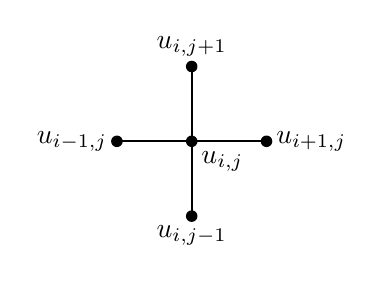
\begin{tikzpicture}[scale=0.95]
  \foreach \x/\y in {0/1,1/0,1/1,1/2,2/1}{\fill (\x,\y) circle (2.2pt);}
  \draw[thick] (0,1)--(2,1);
  \draw[thick] (1,0)--(1,2);
  \node[below] at (1,0) {$u_{i,j-1}$};
  \node[above] at (1,2) {$u_{i,j+1}$};
  \node[left] at (0,1) {$u_{i-1,j}$};
  \node[right] at (2,1) {$u_{i+1,j}$};
  \node[below right] at (1,1) {$u_{i,j}$};
\end{tikzpicture}
\caption{二维五点 stencil。二维化首先改变的是局部邻接：一维的左右两个邻居变成两个坐标方向上的四个邻居。}
\label{fig:discretization-five-point-stencil}
\end{figure}

\subsection{二维局部方程与全局矩阵}

真正需要建立的新心智模型，是二维几何怎样进入一维线性代数向量。先取一个只有 $2\times2$ 个内部未知量的小网格，四周均为齐次 Dirichlet 边界。按
\begin{equation}
\bm u=
\begin{bmatrix}
 u_{1,1}&u_{2,1}&u_{1,2}&u_{2,2}
\end{bmatrix}^{T}
\end{equation}
编号。对四个内部点分别应用式~\eqref{eq:discretization-two-dimensional-five-point}，边界值因为为零直接消失：
\begin{align}
4u_{1,1}-u_{2,1}-u_{1,2}&=h^2f_{1,1},\\
-u_{1,1}+4u_{2,1}-u_{2,2}&=h^2f_{2,1},\\
-u_{1,1}+4u_{1,2}-u_{2,2}&=h^2f_{1,2},\\
-u_{2,1}-u_{1,2}+4u_{2,2}&=h^2f_{2,2}.
\end{align}
于是
\begin{equation}
\boxed{
\frac1{h^2}
\begin{bmatrix}
4&-1&-1&0\\
-1&4&0&-1\\
-1&0&4&-1\\
0&-1&-1&4
\end{bmatrix}
\begin{bmatrix}
u_{1,1}\\u_{2,1}\\u_{1,2}\\u_{2,2}
\end{bmatrix}
=
\begin{bmatrix}
f_{1,1}\\f_{2,1}\\f_{1,2}\\f_{2,2}
\end{bmatrix}.
}
\label{eq:discretization-two-dimensional-small-matrix}
\end{equation}

这个 $4\times4$ 例子暴露了二维化真正新增的结构。矩阵仍然是一行对应一个网格点，但非零元的位置不再只沿主对角线附近连续排列；它们取决于\textbf{二维网格中的几何邻接}以及我们选择的编号方式。

对一般 $n_x\times n_y$ 个内部节点，采用 $x$ 方向先变化的字典序编号
\begin{equation}
p(i,j)=i+n_x(j-1),
\qquad
1\le i\le n_x,
\quad
1\le j\le n_y.
\label{eq:discretization-two-dimensional-indexing}
\end{equation}
于是左右邻居在向量中相差 $1$，上下邻居相差 $n_x$。若网格仍为 $h_x=h_y=h$，把同一条 $x$ 向网格线上的未知量看成一个块，则矩阵具有块三对角结构
\begin{equation}
A_{2D}
=\frac1{h^2}
\begin{bmatrix}
B&-I&&\\
-I&B&\ddots&\\
&\ddots&\ddots&-I\\
&&-I&B
\end{bmatrix},
\qquad
B=\operatorname{tridiag}(-1,4,-1).
\label{eq:discretization-two-dimensional-block-matrix}
\end{equation}
这里的 $B$ 描述同一条水平网格线内部的左右耦合，而块间的 $-I$ 描述相邻两条水平网格线之间的上下耦合。

\begin{keybox}
二维矩阵的块结构不是额外规定出来的。它只是“二维局部邻接 + 一维编号”共同产生的结果。先看懂式~\eqref{eq:discretization-two-dimensional-small-matrix}，再看式~\eqref{eq:discretization-two-dimensional-block-matrix}，就不需要把块三对角结构当成需要背诵的新公式。
\end{keybox}

在这个结构已经清楚以后，矩形网格 $h_x\neq h_y$ 只是把两个方向的权重分开：
\begin{equation}
\boxed{
\frac{2u_{i,j}-u_{i-1,j}-u_{i+1,j}}{h_x^2}
+
\frac{2u_{i,j}-u_{i,j-1}-u_{i,j+1}}{h_y^2}
=f_{i,j}.
}
\label{eq:discretization-two-dimensional-rectangular-grid}
\end{equation}
因此“两个方向具有不同尺度”是对已经理解的二维结构增加不同权重，而不是理解二维离散的起点。

\paragraph{Kronecker 记号。}
若读者熟悉 Kronecker 积，可以把式~\eqref{eq:discretization-two-dimensional-block-matrix}压缩写成
\begin{equation}
A_{2D}=I_y\otimes T_x+T_y\otimes I_x,
\label{eq:discretization-two-dimensional-kronecker}
\end{equation}
其中 $T_x,T_y$ 是对应方向的一维离散算子，$\otimes$ 表示把一维算子组合成块矩阵的 Kronecker 积。这个写法的作用是\textbf{压缩已经理解的结构}，不是建立二维离散所必需的新概念；第一次阅读可以跳过这一式而不影响后文主线。

\subsection{三维七点格式与切片耦合}

三维最自然的入口不是直接写三重索引，而是把计算域看成一叠二维切片。对固定的 $k$，同一个 $z$ 切片内部仍然有二维的四个轴向邻居；此外，每个点还与上一层 $k-1$ 和下一层 $k+1$ 的对应位置耦合。因此在均匀网格上
\begin{equation}
\boxed{
\frac{
6u_{i,j,k}
-u_{i-1,j,k}-u_{i+1,j,k}
-u_{i,j-1,k}-u_{i,j+1,k}
-u_{i,j,k-1}-u_{i,j,k+1}
}{h^2}
=f_{i,j,k}.
}
\label{eq:discretization-three-dimensional-seven-point}
\end{equation}
这就是三维七点格式。

如果一个 $z$ 切片上的二维离散矩阵记为 $A_{xy}$，那么三维系统可以理解为“二维切片之间再形成块三对角耦合”：
\begin{equation}
A_{3D}
=\begin{bmatrix}
A_{xy}+2h^{-2}I&-h^{-2}I&&\\
-h^{-2}I&A_{xy}+2h^{-2}I&\ddots&\\
&\ddots&\ddots&-h^{-2}I\\
&&-h^{-2}I&A_{xy}+2h^{-2}I
\end{bmatrix}.
\label{eq:discretization-three-dimensional-slice-matrix}
\end{equation}
这个式子比直接记一个三重 Kronecker 和更重要：它说明三维并不是“二维公式多两个邻居”而已，而是\textbf{整个二维子系统之间又发生了层间耦合}。

若三个坐标方向的步长分别为 $h_x,h_y,h_z$，则三个方向分别使用对应的逆平方权重：
\begin{align}
(Au)_{i,j,k}
={}&\frac{2u_{i,j,k}-u_{i-1,j,k}-u_{i+1,j,k}}{h_x^2}\\
&+\frac{2u_{i,j,k}-u_{i,j-1,k}-u_{i,j+1,k}}{h_y^2}\\
&+\frac{2u_{i,j,k}-u_{i,j,k-1}-u_{i,j,k+1}}{h_z^2}.
\label{eq:discretization-three-dimensional-rectangular-grid}
\end{align}

把三维网格存进一维数组时当然还需要一个编号，例如
\begin{equation}
p(i,j,k)=i+n_x\bigl[(j-1)+n_y(k-1)\bigr],
\label{eq:discretization-three-dimensional-indexing}
\end{equation}
但这是\textbf{表示层}的问题，而不是七点离散本身的一部分。后面的并行与存储章节会讨论这种编号如何影响连续访问、子域划分和通信；本章此处只需要知道：同一个三维几何邻接在一维向量中会对应不同的索引跨度。

若需要进一步压缩矩阵结构，也可以写成
\begin{equation}
A_{3D}
=I_z\otimes I_y\otimes T_x
+I_z\otimes T_y\otimes I_x
+T_z\otimes I_y\otimes I_x,
\label{eq:discretization-three-dimensional-kronecker}
\end{equation}
但它和二维情形一样只是结构记号；本章的核心是理解“局部七点关系怎样组成切片耦合的全局系统”。

\begin{checkpointbox}
\textbf{即时检查：二维与三维矩阵结构}

回到式~\eqref{eq:discretization-two-dimensional-small-matrix}，逐个指出每个 $-1$ 对应哪一对二维相邻节点。再想象把这个 $2\times2$ 网格复制成两个 $z$ 切片：哪些新增矩阵非零元用于连接两个切片？如果能回答这个问题，就已经掌握了三维切片耦合的核心，而无需先记忆任何 Kronecker 公式。
\end{checkpointbox}




\section{Poisson 的有限体积离散与数值面通量}
\label{sec:discretization-finite-volume}

前两节始终从 Poisson 方程出发，用\textbf{节点型有限差分（finite difference, FD）}近似点上的微分算子。现在保持连续问题不变，只更换离散表示：仍然求解 Poisson 方程，但改用\textbf{单元中心有限体积（cell-centered finite volume, FV）}。本节只讨论规则均匀笛卡尔网格；更一般的网格几何留到后续章节。

这里必须先区分三个对象：连续方程中的\textbf{精确面通量积分}、离散格式中的\textbf{数值面通量}、以及由同一数值面通量在相邻控制体之间反对称装配所得到的\textbf{离散局部守恒}。后文分别用 $Q_{P,f}$ 与 $\widehat Q_{P,f}$ 表示前两者；二者相等只可能出现在特殊解或极限情形中，一般只有一致性意义下的逼近关系。

\subsection{积分恒等式与精确面通量}

仍考虑
\begin{equation}
-\nabla^2u=f.
\label{eq:discretization-poisson-fv-start}
\end{equation}
定义连续通量场
\begin{equation}
\bm q=-\nabla u.
\label{eq:discretization-poisson-flux}
\end{equation}
若 $u\in C^2(\overline V_P)$，则 $\bm q\in C^1(\overline V_P)$，Poisson 方程可写为 $\nabla\cdot\bm q=f$。对控制体 $V_P$ 使用散度定理，得到\textbf{精确积分恒等式}
\begin{equation}
\sum_{f\subset\partial V_P}Q_{P,f}
=
\int_{V_P} f\,\mathrm dV,
\qquad
Q_{P,f}:=\int_f \bm q\cdot\bm n_{P,f}\,\mathrm dA,
\label{eq:discretization-fv-poisson-balance}
\end{equation}
其中 $\bm n_{P,f}$ 是相对于控制体 $P$ 的外法向。注意这里尚未发生离散化：$Q_{P,f}$ 是连续解 $u$ 所决定的精确面通量积分。

若内部面 $f$ 由相邻控制体 $P$ 与 $N$ 共享，则
\begin{equation}
\bm n_{N,f}=-\bm n_{P,f}.
\end{equation}
因此同一个连续通量场在该共享面上满足
\begin{equation}
\boxed{Q_{N,f}=-Q_{P,f}.}
\label{eq:discretization-exact-flux-antisymmetry}
\end{equation}
这是法向定向直接给出的恒等式，而不是经验性的“流出等于流入”。

为了得到代数方程，还必须近似面通量与体积分。若把 $f_P$ 定义为控制体平均
\begin{equation}
\bar f_P:=\frac1{V_P}\int_{V_P}f\,\mathrm dV,
\end{equation}
则右端可以精确写成 $\bar f_PV_P$。实际程序若改用中心点值 $f(\bm x_P)$，这一步就是一个求积近似；对中心对称的规则 cell 且 $f\in C^2$，中点求积满足
\begin{equation}
\int_{V_P}f\,\mathrm dV
=f(\bm x_P)V_P+\Oh(h^2V_P),
\label{eq:discretization-fv-source-quadrature}
\end{equation}
其中 $h$ 表示局部网格尺度。

\subsection{正交网格上的两点数值通量}

现在才引入数值通量。设规则正交网格上的内部面 $f=P|N$ 的中心为 $\bm x_f$，两个 cell center 沿面法向共线，中心距离为 $d_{PN}$，面面积为 $A_f$。以 $P$ 的外法向为定向，定义两点数值通量
\begin{equation}
\boxed{
\widehat Q_{P,f}
:=T_{PN}(u_P-u_N),
\qquad
T_{PN}:=\frac{A_f}{d_{PN}}.
}
\label{eq:discretization-fv-poisson-two-point-flux}
\end{equation}
这里 $u_P,u_N$ 是 cell-centered 离散未知量。在本章的规则均匀网格上，可以把它们理解为对应中心点函数值的近似；若采用 cell-average 作为未知量，对足够光滑的 $u$，中心值与 cell average 的差异同样是二阶量，不改变这里的二阶主阶分析。

式~\eqref{eq:discretization-fv-poisson-two-point-flux}不是由守恒律本身推出的，而是一个\textbf{通量闭合（flux closure）}。在均匀正交网格上，若 $u\in C^3$，以面中心为展开点可得
\begin{equation}
\frac{u_N-u_P}{d_{PN}}
=
\frac{\partial u}{\partial n}(\bm x_f)+\Oh(h^2),
\end{equation}
因此
\begin{equation}
\widehat Q_{P,f}
=Q_{P,f}+\Oh(A_fh^2)
\end{equation}
在面上法向导数足够光滑且面中点求积成立的意义下是一致的。该结论依赖于这里明确给出的正交、对称几何假设；在一般非正交网格上，简单两点公式未必保持同样的一致性阶数。

更重要的是，共享面只能生成\textbf{一个}数值通量，再以相反符号装配到两侧控制体。按同一个 $T_{PN}$ 定义
\begin{equation}
\widehat Q_{N,f}:=T_{PN}(u_N-u_P),
\end{equation}
于是代数上严格有
\begin{equation}
\boxed{
\widehat Q_{N,f}=-\widehat Q_{P,f}.
}
\label{eq:discretization-numerical-flux-antisymmetry}
\end{equation}
当所有内部面都采用这一共享通量约定时，把任意一组相邻控制体的离散方程相加，内部面数值通量会\textbf{精确抵消}。这才是有限体积格式的离散局部守恒性质。它来自数值通量的反对称装配，而不是来自“公式看起来像通量”的直觉。

\begin{figure}[htbp]
\centering
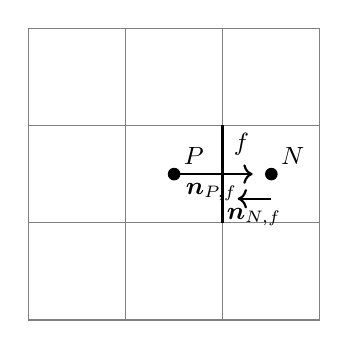
\begin{tikzpicture}[scale=0.95,font=\small]
  \draw[gray] (0,0) grid[step=1.3] (3.9,3.9);
  \fill (1.95,1.95) circle (2.4pt) node[above right] {$P$};
  \fill (3.25,1.95) circle (2.4pt) node[above right] {$N$};
  \draw[very thick] (2.6,1.3)--(2.6,2.6);
  \node[right] at (2.62,2.35) {$f$};
  \draw[->,thick] (1.95,1.95)--(3.0,1.95);
  \node[below] at (2.45,1.95) {$\bm n_{P,f}$};
  \draw[->,thick] (3.25,1.62)--(2.80,1.62);
  \node[below] at (3.02,1.62) {$\bm n_{N,f}$};
\end{tikzpicture}
\caption{共享内部面的定向。连续精确通量满足 $Q_{N,f}=-Q_{P,f}$；离散时若两侧使用同一个共享数值通量，则 $\widehat Q_{N,f}=-\widehat Q_{P,f}$ 也在代数上严格成立。}
\label{fig:discretization-fv-cell-face}
\end{figure}

\subsection{一维 cell-centered Poisson 与一致性}

设一维均匀 cell 宽度为 $h$，第 $i$ 个 cell center 为 $x_i$，左右边界分别为 $x_{i-1/2}$ 与 $x_{i+1/2}$。相对于 cell $i$ 的外法向，数值通量定义为
\begin{align}
\widehat Q_{i,L}&=\frac{u_i-u_{i-1}}{h},\\
\widehat Q_{i,R}&=\frac{u_i-u_{i+1}}{h}.
\end{align}
采用中点求积近似体源，离散平衡写成
\begin{equation}
\widehat Q_{i,L}+\widehat Q_{i,R}=f_i h.
\end{equation}
除以 $h$ 得到
\begin{equation}
\boxed{
\frac{-u_{i-1}+2u_i-u_{i+1}}{h^2}=f_i.
}
\label{eq:discretization-fv-one-dimensional-poisson}
\end{equation}

这一式与节点型中心差分具有相同的代数模板，但其一致性仍需独立验证。把精确解 $u(x_i)$ 代入左端，Taylor 展开给出
\begin{equation}
\frac{-u(x_i-h)+2u(x_i)-u(x_i+h)}{h^2}
=-u''(x_i)-\frac{h^2}{12}u^{(4)}(x_i)+\Oh(h^4).
\end{equation}
因此若 $u\in C^6$，内部离散的局部截断误差为 $\Oh(h^2)$。这说明这里的二阶结论来自 Taylor 展开，而不是来自“FV 与 FD 看起来相同”。

\begin{warningbox}
\textbf{代数模板相同不等于离散对象相同。}

节点型 FD 的未知量位于节点；本节的 cell-centered FV 未知量位于 cell center。即使两者在均匀网格上写出同一个三对角系数模式，它们一般对应不同的物理采样位置。只有在明确给定网格映射、系数位置和右端求积以后，才有资格比较两个离散算子是否代数等价。
\end{warningbox}

\subsection{二维与三维逐面装配}

对二维规则矩形 cell $P$，记四个内部面对应的邻居为 $E,W,N,S$。每个共享面只计算一次数值通量，并按相反符号装配到相邻两个控制体。于是 cell $P$ 的离散方程为
\begin{equation}
\boxed{
\left(T_E+T_W+T_N+T_S\right)u_P
-T_Eu_E-T_Wu_W-T_Nu_N-T_Su_S
=f_PV_P.
}
\label{eq:discretization-fv-poisson-two-dimensional-row}
\end{equation}
在边长为 $h$、单位厚度的均匀正方形网格上，$A_f=h$、$d_{PN}=h$，故 $T_f=1$。再除以 $V_P=h^2$，得到标准五点 Laplacian。这个结论的条件是：规则笛卡尔几何、两点数值通量、中点源项求积以及内部 cell；少掉其中任一条件，都不能直接把“五点格式”当作普遍结论。

三维规则立方体同理，多出上、下两个共享面。若所有六个面都满足同样的正交两点闭合，便得到七点模板。二维到三维真正保持不变的严格结构是：\textbf{每个共享面对应一个反对称的数值通量贡献}；五点或七点只是这一结构在规则笛卡尔网格上的特例。

\subsection{有限差分与有限体积：比较已经证明的内容}

在当前假设下，两种方法可以作如下比较：
\begin{center}
\small
\begin{tabularx}{0.96\textwidth}{>{\bfseries}p{2.7cm}X X}
\toprule
 & 节点型有限差分（FD） & cell-centered 有限体积（FV）\\
\midrule
未知量位置 & 网格节点 & 控制体中心\\
局部方程来源 & 微分算子的差分近似 & 控制体积分恒等式 + 数值面通量闭合\\
首先近似的对象 & 点上的导数 & 面通量积分与体积分\\
二阶结论的依据 & Taylor 截断误差分析 & 通量/求积一致性与等价模板的 Taylor 分析\\
离散局部守恒 & 一般不由“FD”名称自动保证 & 若共享面使用单一反对称数值通量，则严格成立\\
规则 Poisson & 三点/五点/七点 & 在上述假设下得到相同系数模板\\
\bottomrule
\end{tabularx}
\end{center}

下一节把连续模型推广到变系数椭圆算子。届时必须继续区分“连续物理通量”和“人为选择的数值通量”，并检查后者的一致性与共享面反对称性。


\section{从 Poisson 到一般椭圆算子}
\label{sec:discretization-general-elliptic}

考虑标量扩散型算子
\begin{equation}
\mathcal Lu
:=-\nabla\cdot\bigl(\beta(\bm x)\nabla u\bigr)
+\alpha(\bm x)u
=f.
\label{eq:discretization-general-diffusion}
\end{equation}
为了使本节讨论确实处在标准椭圆框架内，先明确基本假设：区域内部取
\begin{equation}
0<\beta_0\le \beta(\bm x)\le \beta_1<\infty,
\qquad
\alpha(\bm x)\ge0,
\label{eq:discretization-ellipticity-assumption}
\end{equation}
并在当前规则网格的一致性分析中假设 $\beta$、$\alpha$ 与精确解具有所需的光滑性。系数跳变时应把问题理解为分片光滑椭圆方程，并额外满足界面条件；该情形不在本节用一个未经证明的“平均公式”代替。

当 $\beta=1$、$\alpha=0$ 时，式~\eqref{eq:discretization-general-diffusion}退化为 Poisson 方程。本节只研究规则均匀笛卡尔网格，目标是严格说明：面/半点系数如何进入离散算子，以及在什么条件下 FD 与 FV 会得到同一代数模板。

\subsection{有限差分：数值半点通量与一致性}

先看一维
\begin{equation}
-\frac{\mathrm d}{\mathrm dx}
\left(\beta(x)\frac{\mathrm du}{\mathrm dx}\right)
+\alpha(x)u
=f.
\label{eq:discretization-general-diffusion-one-dimensional}
\end{equation}
定义连续通量
\begin{equation}
F(x):=-\beta(x)u'(x),
\end{equation}
则方程为 $F'(x)+\alpha(x)u(x)=f(x)$。在均匀节点 $x_i=ih$ 上，定义\textbf{数值半点通量}
\begin{equation}
\widehat F_{i+1/2}
:=-\beta_{i+1/2}\frac{u_{i+1}-u_i}{h},
\label{eq:discretization-fd-variable-face-flux}
\end{equation}
并取离散散度
\begin{equation}
\frac{\widehat F_{i+1/2}-\widehat F_{i-1/2}}{h}
+\alpha_i u_i
=f_i.
\label{eq:discretization-fd-variable-divergence}
\end{equation}

这里的关键不是把 $\widehat F$ 称为“通量”，而是验证它是否一致。若 $u\in C^5$，在半点 $x_{i+1/2}$ 展开可得
\begin{equation}
\frac{u(x_{i+1})-u(x_i)}{h}
=u'(x_{i+1/2})
+\frac{h^2}{24}u^{(3)}(x_{i+1/2})
+\Oh(h^4).
\label{eq:discretization-centered-first-derivative-midpoint}
\end{equation}
若同时
\begin{equation}
\beta_{i+1/2}
=\beta(x_{i+1/2})+\Oh(h^2),
\label{eq:discretization-face-beta-consistency}
\end{equation}
则
\begin{equation}
\widehat F_{i+1/2}
=F(x_{i+1/2})+\Oh(h^2).
\end{equation}
再对相邻半点的通量作中心差分，Taylor 展开得到
\begin{equation}
\frac{\widehat F_{i+1/2}-\widehat F_{i-1/2}}{h}
=F'(x_i)+\Oh(h^2),
\end{equation}
所以在上述光滑性与面系数一致性条件下，内部离散是二阶一致的。

代入数值通量后得到
\begin{equation}
\boxed{
-\frac{\beta_{i-1/2}}{h^2}u_{i-1}
+\left(
\frac{\beta_{i-1/2}+\beta_{i+1/2}}{h^2}
+\alpha_i
\right)u_i
-\frac{\beta_{i+1/2}}{h^2}u_{i+1}
=f_i.
}
\label{eq:discretization-fd-variable-row}
\end{equation}

这也解释了为什么不能把原算子替换为 $-\beta_i u''$：一般有
\begin{equation}
-(\beta u')'=-\beta u''-\beta'u',
\end{equation}
后者比 $-\beta u''$ 多出一阶耦合项。只有当 $\beta$ 为常数时，两者才相同。

二维均匀笛卡尔网格上，对两个坐标方向分别使用同样的半点构造可得
\begin{align}
&-\frac{
\beta_{i+1/2,j}(u_{i+1,j}-u_{i,j})
-\beta_{i-1/2,j}(u_{i,j}-u_{i-1,j})
}{h_x^2} \\
&-\frac{
\beta_{i,j+1/2}(u_{i,j+1}-u_{i,j})
-\beta_{i,j-1/2}(u_{i,j}-u_{i,j-1})
}{h_y^2}
+\alpha_{i,j}u_{i,j}
=f_{i,j}.
\label{eq:discretization-fd-variable-two-dimensional}
\end{align}
其二阶一致性同样依赖于各方向面系数满足相应的二阶近似条件，而不是只由“五点邻接”这一拓扑事实保证。

\subsection{有限体积：精确积分式、数值通量与求积}

对式~\eqref{eq:discretization-general-diffusion} 在控制体 $V_P$ 上积分，得到精确关系
\begin{equation}
\sum_{f\subset\partial V_P}Q_{P,f}
+
\int_{V_P}\alpha u\,\mathrm dV
=
\int_{V_P}f\,\mathrm dV,
\label{eq:discretization-fv-balance-exact-general}
\end{equation}
其中
\begin{equation}
Q_{P,f}
:=-\int_f\beta\nabla u\cdot\bm n_{P,f}\,\mathrm dA
\label{eq:discretization-bc-flux-definition}
\end{equation}
是连续精确面通量积分。

在本章的均匀正交网格上，定义共享内部面的数值通量
\begin{equation}
\boxed{
\widehat Q_{P,f}
:=T_{PN}(u_P-u_N),
\qquad
T_{PN}:=\frac{\beta_fA_f}{d_{PN}}.
}
\label{eq:discretization-fv-two-point-flux}
\end{equation}
这里要求相邻两个控制体对同一面使用同一个 $\beta_f$ 和同一个 $T_{PN}$，从而严格保持
\begin{equation}
\widehat Q_{N,f}=-\widehat Q_{P,f}.
\label{eq:discretization-fv-general-antisymmetry}
\end{equation}
若 $\beta$ 在面附近光滑，$\beta_f=\beta(\bm x_f)+\Oh(h^2)$，且网格正交对称，则该两点通量对精确面通量是二阶一致的。若 $\beta$ 在面上跳变，则必须由界面连续条件和一侧/两侧系数共同构造 $T_{PN}$；本节不把算术平均或调和平均当作无需条件的定理。

对体积分采用中点求积，
\begin{align}
\int_{V_P}\alpha u\,\mathrm dV
&=\alpha_Pu_PV_P+\Oh(h^2V_P),\\
\int_{V_P}f\,\mathrm dV
&=f_PV_P+\Oh(h^2V_P),
\end{align}
于是得到离散控制体方程
\begin{equation}
\sum_{f\subset\partial V_P}\widehat Q_{P,f}
+\alpha_PV_Pu_P
=f_PV_P.
\label{eq:discretization-fv-balance-general}
\end{equation}
这里的等号定义的是\textbf{离散格式}，不是对连续积分式逐项精确替换。

对二维矩形内部 cell $P$，装配四个共享面的数值通量得到
\begin{equation}
\boxed{
\begin{aligned}
&\left(T_E+T_W+T_N+T_S+\alpha_PV_P\right)u_P\\
&\qquad -T_Eu_E-T_Wu_W-T_Nu_N-T_Su_S
=f_PV_P.
\end{aligned}
}
\label{eq:discretization-two-dimensional-flux-row}
\end{equation}
三维规则笛卡尔网格同理增加上、下两个面。只要同一内部面在两侧使用同一个数值通量，局部守恒是代数恒等式；至于该数值通量是否高阶逼近连续通量，则是另一项必须独立验证的一致性问题。

\subsection{FD 与 FV 的代数重合：条件与边界}

一维均匀网格上，若 FD 与 FV 使用同一组 $\beta_{i\pm1/2}$，FV 采用中点体积分求积，并把每个 cell 的积分方程除以体积 $h$，则两者都得到
\begin{equation}
-\frac{\beta_{i-1/2}}{h^2}u_{i-1}
+\left(
\frac{\beta_{i-1/2}+\beta_{i+1/2}}{h^2}
+\alpha_i
\right)u_i
-\frac{\beta_{i+1/2}}{h^2}u_{i+1}
=f_i.
\end{equation}

这是一个有明确前提的代数结论，而不是“FD 与 FV 本质相同”。至少有三点不能由该式推出：第一，节点型 FD 与 cell-centered FV 的未知量通常位于不同物理位置；第二，在非正交网格或不同求积/重构下，两者未必生成同一矩阵；第三，FV 的共享面反对称装配提供离散局部守恒，而一般 FD 格式是否具有相同性质必须从其具体数值通量形式单独检查。

\subsection{零阶项与零空间}

式~\eqref{eq:discretization-general-diffusion} 中的 $\alpha u$ 不产生新的空间邻居。在节点型 FD 中，它给矩阵对角元增加 $\alpha_i$；在 cell-centered FV 的积分方程中，它贡献 $\alpha_PV_P$。因此在当前点值/中点求积离散下，零阶项不改变内部邻接拓扑。

对连通网格上的纯 Neumann Poisson 离散，扩散部分具有常数零空间。若离散的 $\alpha_i\ge0$，且至少一个自由度上 $\alpha_i>0$（FV 中相应为 $\alpha_iV_i>0$），则常数向量不再属于零空间；在对称扩散离散下，这一事实还可通过离散能量式严格证明。后面的线性代数部分会再次使用这一结构。

\subsection{各向异性算子：由交叉导数说明邻接扩大}

若扩散系数推广为对称正定张量 $\bm B$，考虑常系数二维算子
\begin{equation}
-\nabla\cdot(\bm B\nabla u),
\qquad
\bm B=
\begin{bmatrix}
\beta_{xx}&\beta_{xy}\\
\beta_{xy}&\beta_{yy}
\end{bmatrix}.
\end{equation}
直接展开得
\begin{equation}
-\beta_{xx}u_{xx}
-2\beta_{xy}u_{xy}
-\beta_{yy}u_{yy}.
\label{eq:discretization-anisotropic-expanded}
\end{equation}
若 $\beta_{xy}\ne0$，标准二阶中心差分对 $u_{xy}$ 的近似为
\begin{equation}
u_{xy}(x_i,y_j)
\approx
\frac{
u_{i+1,j+1}-u_{i+1,j-1}-u_{i-1,j+1}+u_{i-1,j-1}}{4h_xh_y},
\end{equation}
它显式引入四个对角邻居。因此在坐标轴不与张量主方向对齐时，经典轴向五点 stencil 一般不足以表示这一标准二阶离散。这一结论来自交叉导数的具体离散式，而不是对“各向异性更复杂”的直观判断。

\begin{keybox}
本节需要保留的严格区分是：\textbf{连续通量}由 PDE 定义，\textbf{数值通量}由离散方法选择；共享面数值通量的反对称性保证\textbf{离散守恒}，而数值通量逼近连续通量的阶数决定\textbf{一致性}。这三个概念不能互相替代。
\end{keybox}

\section{边界条件的离散闭合}
\label{sec:discretization-boundary-conditions}

现在节点型 FD 和 cell-centered FV 都已经建立。连续边界条件本身并不会因为离散方法改变，但它进入代数系统的方式取决于\textbf{未知量布局}：FD 可能在边界节点上直接保存 $u$，FV 则通常通过控制体的边界面提供通量闭合。因此本节不再切换离散表示，只研究“同一个边界信息在已经确定的表示中怎样闭合方程”。本节始终沿着同一条链路：
\begin{equation}
\boxed{
\begin{gathered}
\text{连续边界条件}\longrightarrow\text{离散边界关系}\\
\downarrow\\[-0.4em]
\text{消去边界/辅助量}\longrightarrow\text{修改矩阵行与右端}
\end{gathered}
}
\label{eq:discretization-bc-chain}
\end{equation}
先在一维节点型有限差分上把这条链走通，再进入二维、三维。这样多维边界不会变成一组需要背诵的特殊规则。


\subsection{未知量布局与边界表示}

在写任何边界公式之前，先把两种表示放在一起：
\begin{center}
\small
\begin{tabularx}{0.95\textwidth}{>{\bfseries}p{2.8cm}X X}
\toprule
 & 节点型 FD & cell-centered FV\\
\midrule
边界附近未知量 & 边界点可能就是一个 $u_0$ & 最近未知量在边界内侧的 cell center $P$\\
Dirichlet & 可直接给边界节点值，或消去该自由度 & 用已知边界面值闭合 $Q_f$\\
Neumann & 用单边/辅助点关系近似法向导数 & 直接给定边界面通量或由导数换算通量\\
二维角部 & 不同边界段可能落到同一个角节点 & 一个角部 cell 拥有多个物理边界面\\
三维棱/角 & 一个节点可能位于多个边界面的闭包上 & 一个 cell 可同时拥有两个或三个边界面\\
\bottomrule
\end{tabularx}
\end{center}

因此边界条件离散的第一步永远不是“套 Dirichlet/Neumann 公式”，而是先确认当前代数未知量与物理边界之间的几何关系。

\subsection{一维边界闭合}

回到一维 Poisson 方程。第一个内部点满足
\begin{equation}
\frac{-u_0+2u_1-u_2}{h^2}=f_1.
\label{eq:discretization-bc-first-row-open}
\end{equation}
如果 $u_0$ 既不是已知量，也没有包含在未知向量中，这一行就没有闭合。边界条件的数值作用正是补上关于 $u_0$ 的关系。

有两种常见代数布局：
\begin{enumerate}
\item \textbf{消去边界自由度。}未知向量只保存内部点，用边界条件把 $u_0$ 写成内部未知量和已知数据，再代回式~\eqref{eq:discretization-bc-first-row-open}；
\item \textbf{保留边界自由度。}把 $u_0$ 也放进未知向量，并把离散边界条件本身作为矩阵的一行。
\end{enumerate}
本章首先采用第一种方式，因为它与前面的一维未知向量定义一致。第二种方式在需要保留边界节点时也很常见，两者的区别是\textbf{未知量布局}，不是连续边界条件本身发生了变化。

\subsection{Dirichlet 边界条件}

左端 Dirichlet 条件直接给定
\begin{equation}
u_0=g_D.
\end{equation}
代入式~\eqref{eq:discretization-bc-first-row-open}：
\begin{equation}
\boxed{
\frac{2u_1-u_2}{h^2}
=f_1+\frac{g_D}{h^2}.
}
\label{eq:discretization-dirichlet-row}
\end{equation}
所以 Dirichlet 条件没有增加未知量，而是把原来 stencil 中的边界值移入右端。若边界自由度被保留，则还可以直接使用
\begin{equation}
u_0=g_D
\end{equation}
作为边界行；如果后续算法依赖矩阵对称性，强制单位行时还应同时处理对应矩阵列，或者直接消去该自由度。

\subsection{Neumann 边界条件}

Neumann 条件给定外法向导数
\begin{equation}
\frac{\partial u}{\partial n}=g_N.
\label{eq:discretization-neumann-bc}
\end{equation}
左端点的外法向指向 $-x$，因此
\begin{equation}
-u'(0)=g_N.
\end{equation}
用最简单的一阶差分
\begin{equation}
u'(0)\approx\frac{u_1-u_0}{h}
\end{equation}
得到
\begin{equation}
u_0=u_1+h g_N.
\label{eq:discretization-neumann-eliminate-uzero}
\end{equation}
代回第一行：
\begin{equation}
\boxed{
\frac{u_1-u_2}{h^2}
=f_1+\frac{g_N}{h}.
}
\label{eq:discretization-neumann-first-row}
\end{equation}
与 Dirichlet 相比，第一行的对角系数已经发生变化。边界条件因此不仅改变右端，也可能改变矩阵本身。

例如左端取 Neumann、右端取 Dirichlet $u_{N+1}=g_R$。未知向量仍由内部值 $u_1,\ldots,u_N$ 组成，此时矩阵变为
\begin{equation}
\frac1{h^2}
\begin{bmatrix}
1&-1&&&\\
-1&2&-1&&\\
&\ddots&\ddots&\ddots&\\
&&-1&2&-1\\
&&&-1&2
\end{bmatrix}
\begin{bmatrix}
u_1\\u_2\\\vdots\\u_{N-1}\\u_N
\end{bmatrix}
=
\begin{bmatrix}
f_1+g_N/h\\f_2\\\vdots\\f_{N-1}\\f_N+g_R/h^2
\end{bmatrix}.
\label{eq:discretization-mixed-neumann-dirichlet-matrix}
\end{equation}

\paragraph{纯 Neumann 情形。}
若两端都给 Neumann 条件，矩阵两端的对角元都变成 $1/h^2$。齐次情形下常数向量满足
\begin{equation}
A\bm 1=0,
\end{equation}
因此解只确定到一个加法常数。连续方程相应要求兼容条件
\begin{equation}
\boxed{
\int_\Omega f\,\mathrm d\Omega
+\int_{\partial\Omega}g_N\,\mathrm dS=0.
}
\label{eq:discretization-neumann-compatibility}
\end{equation}
这里的零空间不是求解器制造出来的，而是边值问题本身的一部分；后面的迭代方法必须尊重这一结构。

\subsection{Robin 边界条件}

Robin 条件给定函数值与外法向导数的局部线性组合：
\begin{equation}
a u+b\frac{\partial u}{\partial n}=g.
\label{eq:discretization-robin-general}
\end{equation}
仍看左端。用
\begin{equation}
\frac{\partial u}{\partial n}
\approx
\frac{u_0-u_1}{h}
\end{equation}
得到
\begin{equation}
(ah+b)u_0-bu_1=gh,
\end{equation}
于是
\begin{equation}
\boxed{
u_0=\frac{b}{ah+b}u_1+\frac{gh}{ah+b}.
}
\label{eq:discretization-robin-boundary-value}
\end{equation}
代回式~\eqref{eq:discretization-bc-first-row-open}：
\begin{equation}
\boxed{
\frac{2ah+b}{h^2(ah+b)}u_1
-\frac1{h^2}u_2
=f_1+\frac{g}{h(ah+b)}.
}
\label{eq:discretization-robin-matrix-row}
\end{equation}
当 $b=0$ 时得到 Dirichlet 型闭合；当 $a=0$ 时得到 Neumann 型闭合。这个极限检查比死记 Robin 行更重要，因为它能直接发现符号或法向约定写错的问题。

到这里，一维中最常见的三种局部边界条件已经完成了同一件事：\textbf{把缺失的边界信息转化成一条闭合的矩阵行。}

\begin{warningbox}
\textbf{边界闭合的精度必须单独检查。}

上面的 Neumann 和 Robin 推导刻意使用一阶单边导数，只为了让“边界关系怎样进入矩阵行”完全透明。它并不自动与内部二阶中心差分组成整体二阶格式。若目标是保持二阶精度，应改用二阶单边差分、与目标阶数一致的边界闭合，或在有限体积中采用与目标阶数一致的边界通量重构。\textbf{内部 stencil 的阶数不能替代边界离散的阶数检查。}
\end{warningbox}

\subsection{二维边界段与角点}

二维新增的困难不是“多写一个 $y$ 方向导数”，而是\textbf{不同边界段会在角点相遇}。先继续使用前面的节点型有限差分布局。设矩形区域的西、东、南、北四条边分别记为
\begin{equation}
\Gamma_W,\quad\Gamma_E,\quad\Gamma_S,\quad\Gamma_N.
\end{equation}
每一条开放边界段内部都可以使用前面的一维法向离散；真正的新问题出现在边界段的交界。

\paragraph{两个 Dirichlet 边界相交。}
若西边给
\begin{equation}
u(0,y)=g_W(y)
\end{equation}
而南边给
\begin{equation}
u(x,0)=g_S(x),
\end{equation}
那么左下角只有一个几何点 $(0,0)$。如果要求连续解具有连续的边界迹（trace，即把域内解限制到边界后得到的值），自然需要
\begin{equation}
g_W(0)=g_S(0).
\label{eq:discretization-dirichlet-corner-compatibility}
\end{equation}
在节点型离散中，角点也只对应一个节点，因此程序最终必须给它一个唯一值。需要注意的是：如果只要求积分意义上的弱解，单个几何角点的数据不一定像整段边界数据那样决定域内解；本章不展开这一函数空间问题。对离散程序而言，只要网格显式保存该角点，就仍然必须给它一个唯一、明确的离散值。

\paragraph{Dirichlet 与 Neumann 相交。}
若西边是 Dirichlet、南边是 Neumann，一个常见的节点型约定是：角点值由 Dirichlet 条件确定，而 Neumann 条件施加在南边界除该角点以外的边界节点上。比如南边界外法向为 $-y$，用一阶法向差分时，对 $i\ge1$ 的南边界节点可写
\begin{equation}
u_{i,0}=u_{i,1}+h\,g_S(x_i),
\end{equation}
而左下角直接取
\begin{equation}
u_{0,0}=g_W(0).
\end{equation}
这样不会给同一个角点未知量同时写两条独立边界行。这个规则是\textbf{离散约定}，不是所有方法都必须采用的唯一处理方式；有限元、有限体积或不同的边界辅助点构造可以采用不同布局。

\paragraph{边界类型改变与解的光滑性。}
即使每条边界数据本身合法，Dirichlet--Neumann 或 Dirichlet--Robin 的切换点也可能降低局部正则性（也就是解的光滑程度）；几何再入角会进一步加强这种效应。第一章不展开椭圆正则性理论，只保留一个数值后果：\textbf{内部 stencil 是二阶的，并不自动保证含边界交界的整个问题仍表现出理想的二阶全局收敛。}验证时必须把交界附近误差也包含在网格收敛测试中。

三维的结构是同一问题的进一步提升：边界条件定义在二维面上，两个面在棱上相遇，三个面在角点相遇。节点型离散若显式保存这些棱/角节点，就必须给出一致的交界约定；这不是把二维角点规则逐字复制三遍，而是同一个未知量可能同时落在更多边界片段的闭包上。

\begin{figure}[htbp]
\centering
\begin{tikzpicture}[scale=0.88,font=\small]
  % nodal panel
  \begin{scope}[xshift=0cm]
    \draw[very thick] (0,0)--(0,2.2);
    \draw[very thick] (0,0)--(2.2,0);
    \foreach \x in {0,0.8,1.6}{
      \foreach \y in {0,0.8,1.6}{\fill (\x,\y) circle (2pt);}
    }
    \draw[gray] (0,0.8)--(1.6,0.8) (0,1.6)--(1.6,1.6)
                (0.8,0)--(0.8,1.6) (1.6,0)--(1.6,1.6);
    \filldraw[fill=white,draw=black,thick] (0,0) circle (3.4pt);
    \node[above left] at (0,0) {角节点};
    \node[left] at (0,1.25) {$\Gamma_D$};
    \node[below] at (1.2,0) {$\Gamma_N$};
    \node at (0.8,-0.65) {节点型：保存角节点};
  \end{scope}
  % cell-centered panel
  \begin{scope}[xshift=5.4cm]
    \draw[very thick] (0,0)--(0,2.2);
    \draw[very thick] (0,0)--(2.2,0);
    \draw[gray] (0,1)--(2,1) (1,0)--(1,2) (0,2)--(2,2) (2,0)--(2,2);
    \foreach \x/\y in {0.5/0.5,1.5/0.5,0.5/1.5,1.5/1.5}{\fill (\x,\y) circle (2.2pt);}
    \node[above right] at (0.5,0.5) {$P$};
    \node[above right] at (1.5,0.5) {$E$};
    \node[above right] at (0.5,1.5) {$N$};
    \node[left] at (0,0.5) {$f_W$};
    \node[below] at (0.5,0) {$f_S$};
    \node at (1.0,-0.65) {cell-centered：边界面闭合};
  \end{scope}
\end{tikzpicture}
\caption{同一个二维物理角在两种离散布局中的不同代数对象。左：节点型有限差分显式保存角节点；右：cell-centered 有限体积没有角点未知量，角部控制体 $P$ 通过西、南两个边界面接收边界贡献。}
\label{fig:discretization-corner-layouts}
\end{figure}

\begin{center}
\footnotesize
\begin{tabularx}{0.92\textwidth}{>{\bfseries}p{3.0cm}X X}
\toprule
二维交界 & 节点型离散需要决定什么 & 连续/数值上应检查什么\\
\midrule
Dirichlet--Dirichlet & 同一个角节点只能取一个值 & 经典连续 trace 是否一致；离散数据冲突时必须给出唯一约定\\
Dirichlet--Neumann/\newline Robin & 常见做法是由 Dirichlet 固定角节点，另一条件作用于开放边界段 & 交界附近正则性与整体收敛阶\\
Neumann--Neumann & 两条边给出不同法向分量，角节点仍需具体 closure & 全局兼容条件、角部离散精度与零空间\\
Robin--Robin /\newline Neumann--Robin & 一个节点同时邻接两条局部边界关系 & 采用何种角点方程必须由离散布局明确，而不能机械叠加两条矩阵行\\
\bottomrule
\end{tabularx}
\end{center}

\subsection{cell-centered 有限体积中的边界面}
\label{sec:discretization-cell-centered-boundary}

对边界 cell，连续精确通量仍定义为
\begin{equation}
Q_{P,f}=-\int_f\beta\frac{\partial u}{\partial n}\,\mathrm dA,
\end{equation}
其中法向始终取\textbf{相对于控制体 $P$ 的外法向}。边界条件的作用，是给这个缺少相邻 cell 的面提供一个数值通量 $\widehat Q_{P,f}$。为了避免符号混乱，下面所有 Neumann 数据 $g_N$ 均定义为
\begin{equation}
\frac{\partial u}{\partial n}=g_N
\end{equation}
中的\textbf{外法向导数}；因此对应的连续外向扩散通量是 $-\beta g_N$，不是 $+\beta g_N$。

\paragraph{Dirichlet 面：一侧两点闭合。}
若边界面给定 $u_f=g_D$，cell center 到边界面的法向距离为 $\delta_f$，最简单的两点闭合是
\begin{equation}
\widehat Q_{P,f}
=T_f(u_P-g_D),
\qquad
T_f=\frac{\beta_fA_f}{\delta_f}.
\label{eq:discretization-bc-dirichlet-numerical-flux}
\end{equation}
这只是一个数值通量定义。若 $u_P$ 解释为中心点值，则 $(g_D-u_P)/\delta_f$ 对边界法向导数通常只有一阶一致性；因此不能仅凭内部二阶 stencil 宣称整个边值问题二阶收敛。高阶边界闭合必须另行构造和分析。

\paragraph{Neumann 面：通量由边界数据直接给出。}
若 $\partial_nu=g_N$，并以面中点值代表边界数据，则
\begin{equation}
\boxed{
\widehat Q_{P,f}=-\beta_fA_fg_N.
}
\label{eq:discretization-bc-neumann-numerical-flux}
\end{equation}
若 $g_N$ 或 $\beta$ 沿面变化，更严格的表达应是对 $-\beta g_N$ 的面求积；上式本身包含中点求积近似。

考虑二维左下角控制体 $P$：西面为 Dirichlet $u=g_D$，南面为 Neumann $\partial_nu=g_N$，东、北分别邻接内部 cell $E,N$。将四个面的数值通量代入
\begin{equation}
\sum_f\widehat Q_{P,f}+\alpha_PV_Pu_P=f_PV_P
\end{equation}
得到
\begin{equation}
\boxed{
\begin{aligned}
&\left(T_{PE}+T_{PN}+T_W+\alpha_PV_P\right)u_P
-T_{PE}u_E-T_{PN}u_N\\
&\qquad =f_PV_P+T_Wg_D+\beta_SA_Sg_N.
\end{aligned}
}
\label{eq:discretization-mixed-corner-row}
\end{equation}
右端出现 $+\beta_SA_Sg_N$ 的原因不是人为规定符号，而是 Neumann 面的外向数值通量为 $-\beta_SA_Sg_N$，移到方程右端后符号改变。

\paragraph{一般仿射边界闭合。}
若边界面数值关系可写成
\begin{equation}
u_f=c_fu_P+s_f,
\label{eq:discretization-bc-affine-closure}
\end{equation}
并仍采用
\begin{equation}
\widehat Q_{P,f}
=T_f(u_P-u_f),
\qquad
T_f=\frac{\beta_fA_f}{\delta_f},
\label{eq:discretization-bc-transmissibility}
\end{equation}
则代数上严格有
\begin{equation}
\widehat Q_{P,f}
=T_f(1-c_f)u_P-T_fs_f.
\end{equation}
把已知项移到右端后，该边界面对矩阵与右端的贡献为
\begin{equation}
\boxed{
\Delta A_{PP}=T_f(1-c_f),
\qquad
\Delta b_P=T_fs_f.
}
\label{eq:discretization-bc-general-matrix-contribution}
\end{equation}
这只是给定离散边界闭合后的代数恒等式；其准确度由 $u_f=c_fu_P+s_f$ 本身的截断误差决定。

对 Robin 条件
\begin{equation}
a_fu_f+b_f\frac{\partial u}{\partial n}=g_f,
\end{equation}
若使用一阶法向近似
\begin{equation}
\frac{\partial u}{\partial n}
\approx\frac{u_f-u_P}{\delta_f},
\end{equation}
且 $a_f\delta_f+b_f\ne0$，则
\begin{equation}
u_f
=\frac{b_f}{a_f\delta_f+b_f}u_P
+\frac{g_f\delta_f}{a_f\delta_f+b_f},
\end{equation}
从而
\begin{equation}
\boxed{
\Delta A_{PP}
=\frac{\beta_fA_fa_f}{a_f\delta_f+b_f},
\qquad
\Delta b_P
=\frac{\beta_fA_fg_f}{a_f\delta_f+b_f}.
}
\label{eq:discretization-robin-matrix-contribution}
\end{equation}
令 $b_f=0$ 可检查 Dirichlet 极限，令 $a_f=0$ 可检查 Neumann 极限；但这种极限检查只能验证代数与符号的一致性，不能替代边界截断误差分析。

对一个控制体 $P$，记 $\mathcal N(P)$ 为内部面邻居集合，$\Gamma(P)$ 为物理边界面集合，则
\begin{equation}
\boxed{
\begin{aligned}
&\left(
\alpha_PV_P
+\sum_{N\in\mathcal N(P)}T_{PN}
+\sum_{f\in\Gamma(P)}\Delta A_f
\right)u_P\\
&\qquad
-\sum_{N\in\mathcal N(P)}T_{PN}u_N
=
f_PV_P
+\sum_{f\in\Gamma(P)}\Delta b_f.
\end{aligned}
}
\label{eq:discretization-general-boundary-row}
\end{equation}
该式是给定内部数值通量与边界数值通量之后的装配公式。它本身不提供收敛阶；收敛阶必须结合内部一致性、边界一致性、稳定性以及问题正则性共同判断。

\begin{keybox}
\textbf{FV 边界面的符号规则只有一条：先固定外法向，再定义外向数值通量。}

Dirichlet、Neumann、Robin 的矩阵符号都应从 $\widehat Q_{P,f}$ 推导，而不是分别背诵。特别地，若 Neumann 数据定义为 $\partial_nu=g_N$，则外向扩散通量为 $-\beta g_N$；将该已知通量移到右端后才出现 $+\beta A g_N$。
\end{keybox}

\subsection{周期边界条件}

周期条件不是给定一个已知边界值或通量，而是把一侧的未知量与另一侧对应位置识别为同一个周期邻居。对一维周期网格，令
\begin{equation}
u_0=u_N,
\qquad
u_{N+1}=u_1.
\end{equation}
则矩阵成为循环三对角结构：
\begin{equation}
\frac1{h^2}
\begin{bmatrix}
2&-1&0&\cdots&-1\\
-1&2&-1&&0\\
0&\ddots&\ddots&\ddots&\vdots\\
\vdots&&-1&2&-1\\
-1&0&\cdots&-1&2
\end{bmatrix}.
\label{eq:discretization-periodic-matrix}
\end{equation}
所以周期条件的代数特征是\textbf{新增跨边界的未知量耦合}，而不是把已知数据移到右端。没有零阶项时，周期 Poisson 与纯 Neumann 一样具有常数零空间。

二维若只在 $x$ 方向周期，每一条固定 $j$ 的网格线都在左右边界之间建立邻接；若 $x,y$ 两个方向都周期，则角部邻接同时跨越两个方向。三维中，一个周期面要按两个切向坐标与对侧面逐点配对；当两个或三个方向同时周期时，来自不同方向的映射还必须在棱和角处组成一致的等价关系。这里的核心仍然是“修改邻接关系”；具体跨边界数据访问与通信实现留到\chapref{ch:parallel-model}之后的并行章节。

\subsection{Dirichlet-to-Neumann 算子}

前面的 Dirichlet、Neumann 和 Robin 都是局部边界关系。DtN 不同：它来自被截去的外部区域，一般把\textbf{整段或整个边界上的函数值}映射为相应的法向响应，因此通常是非局部算子。本小节属于扩展内容；第一次阅读只需掌握“外域可以被消去，并在边界上留下一个矩阵算子”这一点。

为了避免导数与物理扩散通量之间的符号混乱，这里把离散 DtN 直接定义成\textbf{边界值到外向扩散通量}的映射：
\begin{equation}
\bm q_\Gamma
=K_\Gamma\bm u_\Gamma+\bm q_\Gamma^{(0)}.
\label{eq:discretization-discrete-dtn-flux}
\end{equation}
若 $C_\Gamma\bm u$ 提取全局未知量在边界上的 trace，而 $B_\Gamma$ 把边界通量装配进相邻方程，则
\begin{equation}
A_{int}\bm u+B_\Gamma\bm q_\Gamma=\bm b_{int}
\end{equation}
变成
\begin{equation}
\boxed{
\left(A_{int}+B_\Gamma K_\Gamma C_\Gamma\right)\bm u
=
\bm b_{int}-B_\Gamma\bm q_\Gamma^{(0)}.
}
\label{eq:discretization-dtn-matrix-form}
\end{equation}
如果 $K_\Gamma$ 只是逐点乘法，这个边界修改看起来像局部 Robin；一般二维、三维外域中，$K_\Gamma$ 会耦合多个边界自由度，因此边界块可以明显宽于原来的局部 stencil。

\paragraph{一个可精确求出的模型外域。}
为把 DtN 从抽象矩阵变成可手算对象，考虑内部区域 $0<x<L$，
\begin{equation}
-u''=f,
\qquad
u(0)=g_0,
\end{equation}
而外部半直线 $x>L$ 满足
\begin{equation}
-v''+\kappa^2v=0,
\qquad
v(x)\to0\quad(x\to\infty),
\qquad
v(L)=u(L),
\end{equation}
其中 $\kappa>0$。这个 modified Helmholtz 外域被选来作为教学模型，是因为它具有显式衰减解；\textbf{它不是一般静电 Poisson 外域的普遍 DtN 公式。}

外域解为
\begin{equation}
v(x)=u(L)e^{-\kappa(x-L)},
\end{equation}
于是内部区域右端外法向为 $+x$ 时
\begin{equation}
\boxed{
\frac{\partial u}{\partial n}(L)=-\kappa u(L).
}
\label{eq:discretization-dtn-one-dimensional-exact}
\end{equation}
若扩散系数为 $\beta$，对应外向扩散通量为 $q=\beta\kappa u(L)$，因此在前面“值到通量”的定义下，这个一维 DtN 只是标量 $K_\Gamma=[\beta\kappa]$。

下面为了得到一个完整矩阵，\textbf{切换回节点型有限差分}，并让 $u_N$ 本身位于截断边界 $x=L$。取 $x_i=ih$、$L=Nh$，未知向量为
\begin{equation}
\bm u=(u_1,\ldots,u_N)^T.
\end{equation}
内部节点 $i=1,\ldots,N-1$ 使用
\begin{equation}
-u_{i-1}+2u_i-u_{i+1}=h^2f_i,
\end{equation}
而边界导数用一阶后向差分：
\begin{equation}
\frac{u_N-u_{N-1}}{h}=-\kappa u_N.
\end{equation}
因此最后一行是
\begin{equation}
-u_{N-1}+(1+\kappa h)u_N=0,
\end{equation}
完整系统为
\begin{equation}
\boxed{
\begin{bmatrix}
2&-1&0&\cdots&0\\
-1&2&-1&\ddots&\vdots\\
0&\ddots&\ddots&\ddots&0\\
\vdots&\ddots&-1&2&-1\\
0&\cdots&0&-1&1+\kappa h
\end{bmatrix}
\begin{bmatrix}
u_1\\u_2\\\vdots\\u_{N-1}\\u_N
\end{bmatrix}
=
\begin{bmatrix}
h^2f_1+g_0\\h^2f_2\\\vdots\\h^2f_{N-1}\\0
\end{bmatrix}.
}
\label{eq:discretization-dtn-one-dimensional-matrix}
\end{equation}
这个例子说明：外部半无限区域已经从未知量中消失，但它留下了一个边界矩阵行。这里 DtN 恰好具有 Robin 形式，不是因为 DtN 与 Robin 一般等价，而是因为这个一维外域的消去结果恰好是局部标量关系。

\paragraph{外域消元与 Schur 补。}
一般情况下，可以把完整离散系统按内部未知量和外部未知量分块：
\begin{equation}
\begin{bmatrix}
A_{II}&A_{IE}\\
A_{EI}&A_{EE}
\end{bmatrix}
\begin{bmatrix}
\bm u_I\\\bm u_E
\end{bmatrix}
=
\begin{bmatrix}
\bm b_I\\\bm b_E
\end{bmatrix}.
\end{equation}
消去 $\bm u_E$ 得到
\begin{equation}
\boxed{
\left(A_{II}-A_{IE}A_{EE}^{-1}A_{EI}\right)\bm u_I
=
\bm b_I-A_{IE}A_{EE}^{-1}\bm b_E.
}
\label{eq:discretization-dtn-schur}
\end{equation}
这就是 DtN 非局部性的离散来源：即使 $A_{EE}$ 本身稀疏，$A_{EE}^{-1}$ 一般仍是全局的。

\begin{checkpointbox}
\textbf{即时检查：DtN 的一维模型}

只把式~\eqref{eq:discretization-dtn-one-dimensional-exact} 看成边界算子族 $u'(L)+\kappa u(L)=0$，考察 $\kappa\to0^+$ 时最后一行趋向什么局部条件。注意：这只是边界算子族的代数极限；把原来的衰减外域方程直接设成 $\kappa=0$ 会使“任意非零边界值并在无穷远衰减”这一外域问题退化。
\end{checkpointbox}

\subsection{边界条件对线性系统的影响}

现在可以把本节压缩成一张代数地图：
\begin{center}
\small
\begin{tabularx}{0.96\textwidth}{>{\bfseries}p{2.5cm}X X}
\toprule
边界类型 & 闭合机制 & 对 $A\bm u=\bm b$ 的主要影响\\
\midrule
Dirichlet & 给定边界值 & 消去后修改相邻行与右端；保留边界节点时可写边界约束行。\\
Neumann & 给定外法向导数/通量 & 通常改变边界附近行并引入已知通量；纯 Neumann 保留常数零空间。\\
Robin & 值与法向导数的局部线性组合 & 同时改变边界附近矩阵系数和右端。\\
Periodic & 把对侧位置识别为邻居 & 新增跨边界 off-diagonal coupling；多方向周期还要求角/棱映射一致。\\
DtN & 用外域消元得到边界算子 & 一般产生非局部边界耦合，可理解为外域 Schur 补。\\
\bottomrule
\end{tabularx}
\end{center}

\begin{keybox}
\textbf{边界条件最终必须回答两个问题：}

第一，连续边界信息怎样闭合靠近边界的离散方程？

第二，闭合以后究竟修改了哪些未知量、矩阵系数、右端项、零空间或邻接关系？

二维和三维真正新增的难点，是多个边界片段会在角、棱处相遇，而且不同离散布局对这些几何对象的表示不同。
\end{keybox}



\section{离散线性系统的结构性质}

\subsection{稀疏性}

到这里，我们已经用 FD 与 FV 两种表示离散了 Poisson，并把两条路线都推广到变系数椭圆算子，再加入多种边界闭合。现在从线性代数视角检查这些离散系统共同保留下来的结构。对最基本的一维 Poisson，若有 $N$ 个内部点，矩阵尺寸是 $N\times N$，但三点 stencil 使每一行通常只有三个非零元素；二维五点与三维七点格式也只耦合有限数量的邻居。一般变系数算子虽然会改变局部系数，只要离散仍保持局部耦合，稀疏结构就会保留下来。

这种“矩阵尺寸很大，但绝大部分元素都是零”的结构称为\textbf{稀疏（sparse）}。例如三维 $100^3$ 网格有
\begin{equation}
N=10^6
\end{equation}
个未知量。若把 $A$ 当成普通稠密矩阵，它有 $10^{12}$ 个位置；而七点 stencil 真正产生的非零耦合数量只有 $\Oh(N)$ 量级。

因此稀疏性不是某种存储技巧人为制造出来的，而是 PDE 局部性的全局线性代数表现：\textbf{一个局部微分算子只把每个未知量与有限数量的邻居耦合，所以组装后的大矩阵仍然只含有限数量的局部连接。}

这个结论也解释了为什么上一节的边界条件会影响稀疏结构。普通 Dirichlet、Neumann、Robin 和周期条件只增加或修改有限范围内的耦合；而精确 DtN 一般是非局部的，离散后可能在边界自由度之间引入远距离耦合，使边界块比普通 stencil 更稠密。

\subsection{对称性}

回到一维 Dirichlet Poisson 的矩阵。式 \eqref{eq:discretization-matrix-five} 中
\begin{equation}
A^T=A.
\end{equation}
也就是说，$A_{ij}=A_{ji}$。这称为\textbf{对称矩阵（symmetric matrix）}。

这一性质可以直接由装配式验证：若内部共享面 $f=P|N$ 使用同一个 $T_{PN}=T_{NP}$，则 $P$ 行中 $N$ 列与 $N$ 行中 $P$ 列都等于 $-T_{PN}$。因此在未按不同 cell 体积重新缩放各行、且边界消元保持对称处理的前提下，内部面装配保留矩阵对称性。若对不同体积的控制体逐行除以 $V_P$，Euclidean 内积下的矩阵一般不再由这一论证自动保证对称；此时应转而考察加权内积或重新缩放后的算子。

边界实现却可能改变这一性质。例如保留 Dirichlet 边界自由度时，如果只把边界行强行替换成单位行，却不相应消去或修改其他行中的该边界列，那么得到的代数矩阵一般不再对称。需要 SPD 结构时，通常使用自由度消去或对行、列进行一致的对称处理。由此可见，\textbf{“连续算子自伴”并不保证任何随手写出的边界矩阵都自动对称。}

\subsection{正定性与半正定性}

对任意非零向量 $\bm x\in\R^N$，若
\begin{equation}
\bm x^TA\bm x>0,
\qquad \bm x\neq0,
\end{equation}
则称 $A$ 为\textbf{正定矩阵（positive definite）}。

对于一维 Dirichlet Poisson 的三对角矩阵，去掉共同的 $1/h^2$ 后有
\begin{equation}
\bm x^TA\bm x
=\frac1{h^2}\left[
 x_1^2
 +\sum_{i=1}^{N-1}(x_{i+1}-x_i)^2
 +x_N^2
\right].
\label{eq:discretization-discrete-energy}
\end{equation}
右边是若干平方项之和。只要 $\bm x\neq0$，该表达式就严格大于零。因此这个矩阵既对称又正定，简称\textbf{SPD（symmetric positive definite）}。

对于带 Dirichlet 边界的标准 Poisson 离散，上式给出严格正定性。纯 Neumann 情形则不同：常数向量属于零空间，因此二次型可以等于零但不会为负，此时离散算子是\textbf{对称半正定（symmetric positive semidefinite）}。这与前面纯 Neumann 问题“解只确定到一个常数”的结论是同一件事在线性代数中的表达。

本章只需要掌握对称、正定与半正定的基本含义。它们为什么会影响迭代方法和多重网格收敛，将在后续章节真正需要时再讨论。

\begin{checkpointbox}
\textbf{即时检查}

根据式 \eqref{eq:discretization-discrete-energy}，为什么 Dirichlet Poisson 不可能存在一个非零向量 $\bm x$ 使 $A\bm x=0$？提示：若 $A\bm x=0$，则 $\bm x^TA\bm x$ 等于多少？
\end{checkpointbox}


\section{显式矩阵与 Matrix-Free 算子}

得到 $A\bm u=\bm b$ 后，程序必须回答一个非常具体的问题：\textbf{应用 $A$ 时，算子信息究竟存在哪里？}显式矩阵和 matrix-free 的差异，本质上是两种不同的算子表示方式，而不是两个不同的数学问题。

\subsection{显式稀疏矩阵的存储对象}

显式方法把非零矩阵系数真正保存下来。以常见的 CSR（Compressed Sparse Row）思想为例，一个稀疏矩阵至少需要三类数组：
\begin{enumerate}
\item \texttt{values}：所有非零矩阵元素的数值；
\item \texttt{column\_index}：每个非零元素属于哪一列；
\item \texttt{row\_pointer}：每一行的非零元素在前两个数组中的起止位置。
\end{enumerate}

对三维七点离散，内部行大约有七个非零元素。若有 $N$ 个未知量，则
\begin{equation}
\mathrm{nnz}\approx7N,
\end{equation}
其中 $\mathrm{nnz}$ 表示 nonzeros，即非零元素总数。边界会让实际数量略小，但不改变量级。

显式矩阵的优势是结构完全自描述：一个通用稀疏线性代数程序只看这些数组，就能知道每个未知量与哪些列耦合、耦合系数是多少。代价是：\textbf{不仅要存系数，还要存“这些系数属于哪里”的索引信息。}

对于规则 stencil，也可以采用固定对角线、固定邻居等更紧凑的显式格式，从而省掉部分索引。但只要把每个局部系数预先物化并长期保存，它仍属于显式算子表示。

\subsection{Matrix-Free 的存储对象}

Matrix-free 不保存通用的 $(A_{ij})$ 非零列表，而是保存“生成这些局部系数所需要的信息”，并在应用算子时现场计算。

三维常系数 Poisson 是最极端的例子。若网格间距固定，算子只需要知道
\begin{equation}
h_x,\quad h_y,\quad h_z
\end{equation}
以及边界条件等少量元数据，就可以从固定七点公式计算 $Au$。此时没有必要保存 $7N$ 个系数，更没有必要保存 $7N$ 个列索引。

但 matrix-free 并不等于“算子不占内存”。对更一般的式 \eqref{eq:discretization-general-diffusion}，可能仍需保存：
\begin{itemize}
\item cell-centered 的 $\alpha_i$；
\item 各方向 face-centered 的 $\beta$；
\item 网格尺寸或几何信息；
\item 边界类型、边界值或边界 mask；
\item 不规则几何下的体积分数、面积分数或其他局部几何系数。
\end{itemize}
区别在于，这些数据描述的是\textbf{物理/几何系数}，而不是每一个矩阵非零元及其列号。

\begin{keybox}
\textbf{两种表示方式到底存什么：}

显式稀疏矩阵存“已经组装好的代数耦合”：$A_{ij}$ 及其稀疏位置。

Matrix-free 存“生成代数耦合所需的规则和系数”：网格、材料参数、边界与局部几何；$A_{ij}$ 在执行 $Au$ 时临时产生。
\end{keybox}

\subsection{算子存储与工作向量}

比较内存时必须把两类东西分开：
\begin{equation}
\boxed{
\text{总内存}
=\text{算子表示}
+\text{未知量/右端/残差等工作向量}
+\text{求解器额外工作区}.
}
\end{equation}

无论显式还是 matrix-free，至少都要保存未知量 $u$ 和右端 $b$。迭代求解时通常还会有残差 $r=b-Au$、临时向量和其他求解器工作区；残差与迭代修正将在\chapref{ch:iterative-smoothing}正式建立。因此不能把“matrix-free 不存矩阵”误解成“整个求解只需要一个 $u$ 数组”。

为了把问题说清楚，先只比较单层三维七点问题，并假设所有标量均为 FP64，即每个数占 $8$ byte。

若保留四个 cell-centered 向量
\begin{equation}
u,\quad b,\quad r,\quad w,
\end{equation}
其共同内存为
\begin{equation}
M_{vec}=4\times8N=32N\ \text{byte}.
\label{eq:discretization-vector-memory}
\end{equation}
这部分是两种表示都可能需要的共同成本。

\subsection{三维七点算子的存储预算}

现在给出一个具体预算。取
\begin{equation}
N=256^3=16{,}777{,}216
\end{equation}
个未知量。忽略边界辅助层、内存对齐、容器元数据和求解器额外工作区，只估算最核心的数据。

\paragraph{显式 CSR。}
假设内部每行近似 $7$ 个非零元，矩阵数值用 FP64，列索引用 32-bit integer，row pointer 用 64-bit integer。则
\begin{align}
M_{value}
&\approx7N\times8
=56N\ \text{byte}, \\
M_{col}
&\approx7N\times4
=28N\ \text{byte}, \\
M_{row}
&\approx(N+1)\times8
\approx8N\ \text{byte}.
\end{align}
所以仅矩阵本身约为
\begin{equation}
\boxed{
M_{CSR}\approx92N\ \text{byte}
}
\label{eq:discretization-csr-memory}
\end{equation}
代入 $N=256^3$，约为
\begin{equation}
896\ \mathrm{MiB}
+448\ \mathrm{MiB}
+128\ \mathrm{MiB}
=1472\ \mathrm{MiB}
\approx1.44\ \mathrm{GiB}.
\end{equation}
再加式 \eqref{eq:discretization-vector-memory} 中四个工作向量的 $512\ \mathrm{MiB}$，已经接近
\begin{equation}
1.94\ \mathrm{GiB}.
\end{equation}
这还没有计算边界辅助层、内存对齐、容器元数据或求解器额外工作区。

\paragraph{常系数 Matrix-Free。}
对规则三维 Poisson，算子本身只需要少量网格步长和边界元数据。与 $N$ 成正比的主要成本就是工作向量，因此上述四个 FP64 向量约为
\begin{equation}
\boxed{512\ \mathrm{MiB}}.
\end{equation}
与通用 CSR 相比，差异并不是“少了七个浮点数”这么简单，还同时少了列索引和行指针。

\paragraph{变系数 Matrix-Free。}
若保存一个 cell-centered $\alpha$ 和三个方向的 face-centered $\beta$，在大规则三维网格上可粗略估为
\begin{equation}
N+3N=4N
\end{equation}
个 FP64 系数，即约
\begin{equation}
32N\ \text{byte}=512\ \mathrm{MiB}.
\end{equation}
再加四个工作向量，总核心数据约为
\begin{equation}
1.0\ \mathrm{GiB}.
\end{equation}
这已经明显高于常系数 matrix-free，却仍低于上述通用 CSR 示例。若 $\beta$ 是常数，则三个面系数数组又可以退化为少量标量。

\begin{table}[htbp]
\centering
\small
\begin{tabularx}{0.94\textwidth}{>{\raggedright\arraybackslash}p{3.7cm}
                                  >{\raggedright\arraybackslash}X
                                  >{\raggedleft\arraybackslash}p{2.4cm}}
\toprule
表示方式 & 主要存储对象 & $256^3$ 示例\\
\midrule
显式 CSR 算子 & 非零值、列索引、行指针 & 约 $1.44\ \mathrm{GiB}$\\
四个公共工作向量 & $u,b,r,w$ & $0.50\ \mathrm{GiB}$\\
常系数 matrix-free 算子 & 网格步长、边界等少量元数据 & 相对可忽略\\
变系数 matrix-free 算子 & $\alpha$ 与三个方向 face coefficient & 约 $0.50\ \mathrm{GiB}$\\
\bottomrule
\end{tabularx}
\caption{三维七点问题的核心存储预算。该表刻意不计边界辅助层、内存对齐、容器元数据和求解器额外工作区，因此是理解量级的预算而非具体程序的峰值 RSS。}
\label{tab:discretization-storage-budget}
\end{table}

\begin{warningbox}
\textbf{不要把上述预算当成任何库的固定内存公式。}
索引宽度、边界行、稀疏格式、系数是否共享、边界辅助层宽度、工作向量数量和求解器额外工作区都会改变实际 RSS。这里的目标是建立预算方法：先数“每个未知量需要多少 value、多少 index、多少辅助向量”，再乘以 $N$。
\end{warningbox}

\subsection{表示方式的工程取舍}

显式矩阵的主要优势是通用性。矩阵一旦组装完成，许多不依赖几何信息的稀疏线性代数算法可以直接使用它；如果同一个矩阵会被反复求解，组装成本也可以摊薄。

Matrix-free 的主要优势是减少算子存储和内存流量，并避免把一个本来由简单局部公式定义的算子重复编码成“数值 + 索引”。代价是每次应用算子时需要重新计算局部系数或 stencil；而某些只接受显式矩阵的代数算法也无法直接使用。

因此二者不是“先进方法与落后方法”的关系。判断标准是：
\begin{equation}
\boxed{
\begin{gathered}
\text{算子结构是否可由较少的几何/物理信息重建，}\\
\text{以及后续算法是否必须访问显式矩阵条目。}
\end{gathered}
}
\end{equation}

对规则低阶 Poisson/扩散算子，matrix-free 往往非常自然；对一般非结构稀疏系统，显式稀疏矩阵则提供更通用的接口。后面的性能章节还会进一步看到：存储预算不仅决定“能不能装进内存”，也决定一次 $Au$ 需要从内存系统搬运多少字节。


\begin{keybox}
\textbf{关于局部网格细化的前向提示：}本章所有 stencil 都建立在同一离散层上。如果只在局部区域使用更细的网格，新的困难不只是把 $h$ 换成更小的数；粗、细网格会在分辨率交界处相遇，必须重新回答“界面通量如何守恒”“细网格缺失的邻居值从哪里来”“被细网格覆盖的粗网格未知量是否仍是独立自由度”等问题。\chapref{ch:amr-discretization}将从这些问题出发构造自适应网格上的复合离散系统。
\end{keybox}

\section{本章小结}

本章建立了“连续方程--离散算子--线性系统”的完整链条。关键术语如下：

\begin{center}
\begin{tabularx}{0.94\textwidth}{>{\bfseries}p{3.0cm}X}
\toprule
术语 & 本章需要掌握的含义\\
\midrule
网格（grid） & 用有限个空间位置代表连续区域。\\
stencil & 一个网格点的离散方程依赖哪些邻居，以及这些邻居以什么局部系数参与。\\
离散化 & 把连续微分方程转化为有限个代数方程。\\
有限体积（FV） & 从控制体积分恒等式出发，以数值面通量和体积分求积闭合 cell-centered 离散方程。\\
transmissibility & 在给定网格与通量闭合下，把面面积、中心距离和面系数组合成数值面通量权重；其适用性必须由几何与一致性条件保证。\\
稀疏矩阵 & 大部分矩阵元素为零；PDE 局部离散天然产生这种结构。\\
Dirichlet 条件 & 在边界给定函数值。\\
Neumann 条件 & 在边界给定法向导数。\\
Robin 条件 & 在同一边界点给定函数值与法向导数的局部线性组合。\\
DtN 算子（扩展） & 把整个边界上的 Dirichlet 数据映射为相应的 Neumann 数据；一般是非局部边界算子。\\
SPD & 矩阵同时对称且正定。\\
零空间 & 所有满足 $A\bm z=0$ 的向量组成的集合。\\
显式稀疏矩阵 & 保存已经组装好的非零系数及其稀疏位置；CSR 是一种常见表示。\\
Matrix-free（工程扩展） & 不显式保存完整矩阵，而是保存生成局部系数所需的网格、材料与边界信息。\\
一般椭圆算子 & $-\nabla\cdot(\beta\nabla u)+\alpha u=f$；在 $\beta\ge\beta_0>0$ 等条件下属于标准扩散型椭圆算子，离散时必须分别验证面系数/数值通量的一致性。\\
\bottomrule
\end{tabularx}
\end{center}

到这里，读者应能够完成五件可以直接检验的工作。第一，从一维 Poisson 方程推导节点型有限差分并组装小型矩阵；第二，从二维小网格解释五点邻接怎样形成块三对角结构，并把三维看成二维切片之间的进一步耦合；第三，对同一个 Poisson 方程区分精确面通量与数值面通量，从控制体积分恒等式推导 cell-centered FV，并证明共享面数值通量的反对称装配如何给出离散局部守恒；第四，对一般算子 $-\nabla\cdot(\beta\nabla u)+\alpha u=f$，在明确的光滑性、椭圆性与规则网格假设下分别建立 FD 与 FV，并用截断误差说明二阶一致性成立的条件；第五，针对 Dirichlet、Neumann、Robin、周期以及扩展的 DtN，先固定法向与未知量布局，再从离散关系推导矩阵行、右端与零空间，而不是依据直观判断符号和阶数。

在此基础上，变系数算子不再只是“把常数换成数组”：空间变化的 $\beta$ 进入面/半点连接权重，零阶项 $\alpha u$ 则主要增加本地对角贡献。显式矩阵与 matrix-free 一节进一步说明这些数学对象在程序中分别保存什么。具体界面离散、复合网格、迭代求解器、多重网格粗化和并行框架将在后续章节逐步引入。

\section*{习题}

本章习题按“手算离散 $\rightarrow$ 推导结构 $\rightarrow$ 编程验证 $\rightarrow$ 工程判断”组织。计算题应写出中间步骤，不只给最终结论。

\subsection*{计算题}
\begin{enumerate}[label=\arabic*.]
\item 取 $u(x)=e^x$，在 $x=0.5$ 处分别用 $h=0.2,0.1,0.05$ 的三点中心差分近似 $u''(x)$。计算每个 $h$ 下的绝对误差，并用相邻两组误差估计实验收敛阶。
\item 对边值问题
\[
-u''=1,\qquad 0<x<1,\qquad u(0)=0,\quad u(1)=1,
\]
取 $h=1/4$。以三个内部节点值为未知量，写出完整的 $A\bm u=\bm b$，并用消元法求出离散解。将结果与连续精确解在三个节点处比较。
\item 对
\[
-u''=x,\qquad u(0)=1,\qquad u'(1)=2,
\]
取 $h=1/4$。内部点使用二阶中心差分，右端 Neumann 条件使用一阶后向差分。以 $u_1,u_2,u_3,u_4$ 为未知量，逐行写出 $4\times4$ 矩阵和右端向量。
\item 对右端 Robin 条件
\[
2u(1)+3u'(1)=5,
\]
取 $h=1/4$，用一阶后向差分离散导数。把边界方程写成矩阵最后一行；再分别令 Robin 系数退化到纯 Dirichlet 与纯 Neumann，检查矩阵最后一行怎样变化。
\item 对一维截断外域问题，已知精确 DtN 为 $u'(L)=-\kappa u(L)$。取 $L=1$、$h=1/3$、$\kappa=2$、左端 $u(0)=0$，内部方程为 $-u''=1$。写出完整离散线性系统并求解。
\item 在一维均匀网格的某个内部位置，给定 $h=1/2$、$\beta_{i-1/2}=2$、$\beta_{i+1/2}=5$、$\alpha_i=3$。分别从式~\eqref{eq:discretization-fd-variable-row}和 FV 的逐面收支写出该位置的离散行，并比较左右邻居系数、对角系数和右端缩放。
\item 对 $4\times4$ 个内部节点的二维 Poisson 五点离散，采用 lexicographic ordering。写出矩阵的 block-tridiagonal 结构，明确主块和相邻块；计算矩阵阶数与非零元数量。
\item 对一个二维左下角 cell-centered 控制体，西侧给 Dirichlet $u=2$，南侧给外法向 Neumann $\partial_nu=3$，东、北 transmissibility 均为 1，西侧 transmissibility 为 2，南侧 $\beta A=4$，且 $fV=5$。使用式~\eqref{eq:discretization-mixed-corner-row}写出该矩阵行的数值系数和右端。
\item 考虑一个三维 cell-centered 角部控制体 $P$。其东、北、上三个内部面 transmissibility 均为 1；西面为 Dirichlet $u=2$ 且 $T_W=2$；南面为 Neumann $\partial_nu=3$ 且 $\beta A=4$；下面为 Robin $2u+\partial_nu=5$，取 $\delta=1/2$ 且 $\beta A=2$；另有 $fV=1$、$\alpha=0$。逐面计算三个物理边界的矩阵/右端贡献，并写出 $P$ 行。解释为什么这里不是给几何角点写三条独立边界方程。
\item 对 $n_x=n_y=n_z=2$ 的三维内部网格，利用式~\eqref{eq:discretization-three-dimensional-kronecker}写出 $8\times8$ 七点 Poisson 矩阵的块结构，并指出 $x,y,z$ 三个方向邻居在一维编号中的跨度。
\end{enumerate}

\subsection*{推导与证明题}
\begin{enumerate}[label=\arabic*.]
\item 用 Taylor 展开推导三点中心差分二阶导数公式，并严格得到截断误差的 $\Oh(h^2)$ 主项。
\item 从精确积分恒等式~\eqref{eq:discretization-fv-poisson-balance}与数值通量~\eqref{eq:discretization-fv-poisson-two-point-flux}出发，对一维均匀 cell-centered 网格推导式~\eqref{eq:discretization-fv-one-dimensional-poisson}。明确区分 $Q_{P,f}$ 与 $\widehat Q_{P,f}$，并证明式~\eqref{eq:discretization-numerical-flux-antisymmetry}使任意内部共享面在全局求和时精确抵消。最后用 Taylor 展开验证内部离散的二阶局部截断误差。
\item 从式~\eqref{eq:discretization-centered-first-derivative-midpoint}和条件~\eqref{eq:discretization-face-beta-consistency}出发，证明数值半点通量 $\widehat F_{i+1/2}$ 对连续通量 $F(x_{i+1/2})$ 二阶一致，并进一步推导守恒型 FD 行~\eqref{eq:discretization-fd-variable-row}的二阶局部截断误差。再从 FV 离散式~\eqref{eq:discretization-fv-balance-general}说明，在同一均匀网格、同一面系数和同一中点求积下为何会得到相同代数行。
\item 对一维零 Dirichlet Poisson 离散矩阵证明
\[
\bm v^T A\bm v
=\frac{1}{h^2}\sum_i (v_i-v_{i-1})^2>0
\]
对任意非零内部向量成立，从而证明 $A$ 对称正定。
\item 对纯 Neumann Poisson，证明常数向量属于离散矩阵零空间；再从矩阵行求和得到离散兼容条件，并与连续积分兼容条件对应。
\item 从一般边界闭合关系 $u_f=c_fu_P+s_f$ 出发，推导边界面对矩阵对角元与右端项的贡献，并说明 Dirichlet、Neumann、Robin 分别如何落入这一统一形式。
\item 从分块离散系统消去外域自由度，推导 Schur complement，并说明为什么一般 DtN 离散边界块可能是非局部的。
\end{enumerate}

\subsection*{编程与上机题}
\begin{enumerate}[label=\arabic*.]
\item 编写一维 Poisson/扩散装配器，至少支持 Dirichlet、Neumann 和 Robin。对一个有解析解的问题依次取 $N=16,32,64,128$，报告 $L_2$ 与 $L_\infty$ 误差及实验收敛阶。对 Neumann/Robin 边界分别比较一阶单边闭合与二阶边界闭合，判断边界离散是否限制整体收敛阶。
\item 分别实现二维五点 Poisson 的显式稀疏矩阵乘和 matrix-free stencil apply。对随机向量验证两种实现输出一致，并报告误差范数。
\item 给定一组周期的一维 face-centered 系数 $\beta_{i+1/2}$ 和 cell/node-centered $\alpha_i$，分别实现守恒型 FD 与 cell-centered FV 的内部算子装配。让两种实现读取同一组面系数，数值验证它们生成的局部矩阵系数一致；再解释为什么这个实验只验证了规则网格上的代数重合，而没有证明两种方法普遍等价。
\item 构造一个纯 Neumann 离散矩阵，数值验证 $A\bm1\approx0$；再人为给一个不满足兼容条件的右端，观察直接/迭代求解器的表现并解释原因。
\end{enumerate}

\subsection*{工程与综合题}
\begin{enumerate}[label=\arabic*.]
\item 对 $128^3$ 三维七点 Poisson，按 FP64 value、32-bit column index、64-bit row pointer 的 CSR 假设精确估算矩阵存储；再与七系数结构化显式存储、常系数 matrix-free 和四个 FP64 工作向量比较。
\item 给出一个“显式矩阵更合适”和一个“matrix-free 更合适”的实际算子场景。判断时必须从算子信息是否可低成本重建、下游算法是否需要矩阵条目、内存流量三个角度论证。
\item 比较局部 Robin 与一般 DtN 对稀疏结构的影响。若边界有 $M$ 个自由度，一个稠密 DtN 边界块可能引入多少量级的非零元？讨论其对存储与并行通信的后果。
\end{enumerate}

\chapter{有限差分离散方法}
\label{ch:finite-difference}

本章研究如何将连续微分算子转换为离散差分算子。核心路线为
\[
\mathcal{L}(u)\rightarrow \mathcal{L}_h(u_h).
\]

本章将从 Taylor 展开出发，建立差分近似、截断误差、一致性与收敛之间的关系，并讨论椭圆型方程的有限差分离散。

\section{离散思想与网格表示}

\section{Taylor 展开与差分近似}

\section{截断误差、一致性与收敛}

\section{椭圆型方程的有限差分离散}

\section{边界条件离散}

\section{从 stencil 到离散算子}

\chapter{有限体积离散方法}
\label{ch:finite-volume}

本章研究守恒关系如何构造离散模型。有限体积方法从积分形式出发，通过控制体和数值通量保持离散守恒。

核心路线为
\[
\text{守恒律}\rightarrow\text{控制体积分}\rightarrow\text{通量平衡}.
\]

\section{守恒律与积分形式}

\section{控制体离散}

\section{数值通量}

\section{扩散方程的有限体积离散}

\section{有限差分与有限体积的关系}

\chapter{离散算子与稀疏线性系统}
\label{ch:discrete-operator}

本章建立连续算子到代数系统之间的连接：
\[
\mathcal{L}_h u_h=f_h\rightarrow A\bm u=\bm b.
\]

内容包括离散算子结构、稀疏矩阵、对称正定结构、显式矩阵表示以及无矩阵算子表示。

\section{从连续算子到离散算子}

\section{稀疏矩阵结构}

\section{对称性、正定性与能量结构}

\section{显式矩阵与无矩阵算子}

\section{从离散系统到稀疏线性系统}

\chapter{线性系统求解、基本迭代与平滑性质}
\label{ch:iterative-smoothing}

\chapref{ch:discretization}和\chapref{ch:amr-discretization}已经把连续 PDE 变成离散线性系统
\begin{equation}
A\bm u=\bm b.
\end{equation}
从这里开始，问题发生了性质上的变化：离散方程已经给定，接下来要回答的是\textbf{怎样求这个线性系统，以及怎样判断一个求解过程是否真的有效}。在进入 Jacobi、Gauss--Seidel 或 multigrid 之前，本章先建立线性求解方法的基本地图，再深入最简单的平稳迭代，并用误差传播、谱半径、收敛因子和网格依赖性解释它们为什么既“能收敛”，又可能随着网格加密迅速变慢。

本章仍然以一维 Poisson 为最小可检查模型，但分析对象已经提升到代数层。除非特别指出结论依赖局部守恒、对称性、stencil 几何或系数位置，否则误差、残差、stationary iteration 和谱收敛并不要求 $A$ 必须来自 FD 或 FV 中某一种特定构造。

\begin{keybox}
\textbf{本章要建立的主线：}
\[
\boxed{
A\bm u=\bm b
\rightarrow
\text{求解器类型}
\rightarrow
\text{误差/残差}
\rightarrow
\text{局部迭代}
\rightarrow
\text{误差传播}
\rightarrow
\text{收敛速度}
\rightarrow
\text{网格依赖退化}
\rightarrow
\text{平滑性质}
}
\]
第四章的 coarse-grid correction 将由本章最后暴露出的“低频误差难以被局部迭代消除”自然触发。
\end{keybox}

\section{离散线性系统的求解方法地图}
\label{sec:linear-solver-map}

面对
\begin{equation}
A\bm u=\bm b,
\end{equation}
“求解矩阵”并不只有 Jacobi 或 Gauss--Seidel 一条路线。对 PDE 离散产生的大型稀疏系统，至少应先区分四类基本策略；预条件则是横跨多类迭代方法的加速机制。

\subsection{直接法}

直接法通过有限次代数变换把系统化为更容易求解的形式。对一般非奇异矩阵，实际高斯消元通常需要行置换，可写成
\begin{equation}
PA=LU,
\end{equation}
其中 $P$ 是置换矩阵；随后依次求解下三角和上三角系统。若 $A$ 对称正定，则不需要这种行主元选取，可使用 Cholesky 分解
\begin{equation}
A=LL^T.
\end{equation}

“直接”并不意味着浮点计算中绝对没有误差，而是指算法不依赖“第 $k$ 轮近似逐渐趋近真解”这一收敛过程。在精确算术下，分解与回代经过有限步骤即可得到解。

对 PDE 稀疏矩阵，直接法的主要困难是\textbf{fill-in}：原矩阵中为零的位置在消元后可能产生新的非零元，使因子 $L/U$ 比原始 stencil 矩阵稠密得多。因此直接法非常适合中小规模问题、粗层问题或需要重复求解且因子可以复用的场景，但在大规模三维 PDE 上，内存和分解成本可能成为限制。

\subsection{平稳迭代}

另一类方法不一次完成消元，而是从初始猜测 $\bm u^{(0)}$ 出发，重复固定的更新规则。很多方法都可以写成
\begin{equation}
\bm u^{(k+1)}
=
\bm u^{(k)}
+
M^{-1}\left(\bm b-A\bm u^{(k)}\right),
\label{eq:iteration-stationary-preview}
\end{equation}
其中 $M$ 在每一轮保持不变，并且比完整的 $A$ 更容易处理。

Jacobi、weighted Jacobi、Gauss--Seidel 和 SOR 都属于\textbf{平稳迭代（stationary iteration）}。本章会重点研究这一类，因为 Jacobi/GS 不仅可以独立求解小问题，更重要的是它们会成为 multigrid 中的 smoother。

\subsection{Krylov 子空间方法}

Krylov 方法也从初始残差
\begin{equation}
\bm r_0=\bm b-A\bm u^{(0)}
\end{equation}
出发，但它不会每轮机械重复同一个固定修正，而是逐步利用
\begin{equation}
\mathcal K_m(A,\bm r_0)
=
\operatorname{span}
\left\{
\bm r_0,\,
A\bm r_0,\,
A^2\bm r_0,\ldots,
A^{m-1}\bm r_0
\right\}
\label{eq:iteration-krylov-space}
\end{equation}
中累积的信息构造新的近似。

此处只需要建立最低可用认识：Conjugate Gradient（CG）是 SPD 系统的重要代表；GMRES 面向更一般的非对称线性系统。它们的搜索方向和历史信息组织比 stationary iteration 更丰富。后续\chapref{ch:mg-cycles}会在 multigrid 已经形成近似逆以后，正式讨论 CG/GMRES/FGMRES 与 multigrid preconditioner 的组合。

\subsection{多重网格与预条件}

Multigrid 与前两类迭代的核心差异，是显式利用误差的\textbf{尺度结构}：局部平滑器处理细网格上变化快的误差，coarse-grid correction 处理在细网格上变化慢的误差。本章只先建立前半部分的 smoother 机制；\chapref{ch:two-grid}和\chapref{ch:mg-cycles}分别完成 coarse-grid correction 与多层递归。

预条件（preconditioning）则不应被理解成与上述方法平行的“第五种求解器”。它的目标是构造一个容易应用的近似逆
\begin{equation}
M^{-1}\approx A^{-1},
\end{equation}
把原问题变成对迭代算法更友好的形式。Jacobi 的 $D^{-1}$ 可以看成极简单的近似逆；一个完整 V-cycle 则可以成为更强的 multigrid preconditioner。

\begin{table}[htbp]
\centering
\small
\begin{tabularx}{0.96\textwidth}{>{\raggedright\arraybackslash}p{3.0cm}
                                  >{\raggedright\arraybackslash}p{4.5cm}
                                  >{\centering\arraybackslash}p{2.2cm}
                                  >{\raggedright\arraybackslash}X}
\toprule
方法类别 & 核心动作 & 主要信息结构 & 本书中的主要角色\\
\midrule
LU / Cholesky & 分解后做三角求解 & 稀疏因子 $L/U$ & 小规模问题、bottom solve、基准对照\\
Jacobi / GS & 重复固定局部修正规则 & 固定近似矩阵 $M$ & 基本 solver、multigrid smoother\\
CG / GMRES & 在 Krylov 子空间中构造搜索方向 & Krylov 历史与内积 & 大规模外层迭代求解器\\
Multigrid & 在不同尺度上处理不同误差成分 & 层级、transfer 与 coarse operator & solver 或 preconditioner\\
\bottomrule
\end{tabularx}
\caption{本书涉及的主要线性求解路线。这里给出的是角色地图，不替代后续各算法的正式推导。}
\label{tab:iteration-solver-map}
\end{table}

\begin{keybox}
\textbf{本章的范围边界：}
这里不展开 LU pivoting、完整 CG recurrence 或 Arnoldi/GMRES 推导。本章深入 stationary iteration，是因为它既能建立最基本的线性收敛理论，又直接解释 multigrid smoother 为什么有效、为什么又不够。
\end{keybox}

\section{误差、残差与修正方程}

设真解为 $\bm u^\star$，当前近似为 $\bm u^{(k)}$。定义
\begin{equation}
\bm e^{(k)}
=
\bm u^\star-\bm u^{(k)}
\label{eq:iteration-error-def}
\end{equation}
为\textbf{误差（error）}。它直接表示当前解离真解有多远，但实际计算中通常不知道 $\bm u^\star$，因此无法直接计算 $\bm e^{(k)}$。

把当前近似代回原方程，定义
\begin{equation}
\bm r^{(k)}
=
\bm b-A\bm u^{(k)}
\label{eq:iteration-residual-def}
\end{equation}
为\textbf{残差（residual）}。因为 $A\bm u^\star=\bm b$，
\begin{equation}
\bm r^{(k)}
=
A\left(\bm u^\star-\bm u^{(k)}\right)
=
A\bm e^{(k)}.
\label{eq:iteration-residual-error-relation}
\end{equation}
因此残差不是误差本身，而是误差经过算子 $A$ 作用后的结果。

式~\eqref{eq:iteration-residual-error-relation} 还可以反过来读成\textbf{修正方程}：
\begin{equation}
A\,\delta\bm u
=
\bm r^{(k)}.
\label{eq:iteration-correction-equation}
\end{equation}
若能够精确求解它，就有
\begin{equation}
\delta\bm u
=
A^{-1}\bm r^{(k)}
=
\bm e^{(k)},
\end{equation}
于是
\begin{equation}
\bm u^{(k+1)}
=
\bm u^{(k)}+\delta\bm u
=
\bm u^\star.
\end{equation}
所以许多迭代方法都可以理解成：\textbf{用一个比精确求解 $A\delta\bm u=\bm r$ 更便宜的过程，近似构造误差修正。}

例如
\begin{equation}
A=
\begin{bmatrix}
2&-1&0\\
-1&2&-1\\
0&-1&2
\end{bmatrix},
\qquad
\bm b=
\begin{bmatrix}
1\\1\\1
\end{bmatrix},
\qquad
\bm u^{(0)}=\bm0.
\end{equation}
即使不知道真解，也可以立即得到
\begin{equation}
\bm r^{(0)}=\bm b.
\end{equation}
这就是迭代程序实际能够直接观测的量。

\subsection{小残差是否一定意味着小误差}

若 $A$ 可逆，由
\begin{equation}
\bm e=A^{-1}\bm r
\end{equation}
可得
\begin{equation}
\|\bm e\|
\le
\|A^{-1}\|\,\|\bm r\|.
\label{eq:iteration-error-residual-bound}
\end{equation}
因此残差怎样映射成误差，取决于 $A^{-1}$ 的放大能力。

定义矩阵条件数
\begin{equation}
\kappa(A)
=
\|A\|\,\|A^{-1}\|.
\label{eq:iteration-condition-number}
\end{equation}
当 $\bm b=A\bm u^\star\neq0$ 时，可以得到相对量的基本上界
\begin{equation}
\frac{\|\bm e\|}{\|\bm u^\star\|}
\le
\kappa(A)
\frac{\|\bm r\|}{\|\bm b\|}.
\label{eq:iteration-relative-residual-error}
\end{equation}
这并不是说条件数完全决定每一次实际误差，而是说明一个重要事实：\textbf{同样大小的相对残差，在病态系统中可能对应更大的解误差。}

纯 Neumann 问题存在常数零空间时，$A^{-1}$ 在整个空间上不存在；此时必须先进入满足兼容条件并固定 gauge 的可逆子空间，再谈类似的误差--残差关系。

\begin{keybox}
\textbf{三个对象要始终分开：}
\[
\boxed{
\text{error：离真解多远}
\qquad
\text{residual：方程满足得多好}
\qquad
\text{conditioning：二者之间可能放大多少}
}
\]
\end{keybox}

\section{Jacobi 迭代}

\subsection{Jacobi 点迭代公式}

回到一维 Poisson 离散，把共同的 $1/h^2$ 因子乘到右端，一个内部点满足
\begin{equation}
2u_i-u_{i-1}-u_{i+1}
=
h^2f_i.
\label{eq:iteration-point-equation}
\end{equation}
把中心未知量单独写出：
\begin{equation}
u_i
=
\frac12
\left(
h^2f_i+u_{i-1}+u_{i+1}
\right).
\label{eq:jacobi_point}
\end{equation}

如果右侧邻居还不是真解，就用上一轮近似代替。Jacobi 定义为
\begin{equation}
u_i^{(k+1)}
=
\frac12
\left(
h^2f_i
+
u_{i-1}^{(k)}
+
u_{i+1}^{(k)}
\right).
\label{eq:iteration-jacobi-one-dimensional}
\end{equation}
同一轮中所有点只读旧状态 $\bm u^{(k)}$，把结果写入新状态 $\bm u^{(k+1)}$。因此一轮内部没有逐点先后依赖。

\subsection{三未知量离散系统}

取三个内部未知量，两端 Dirichlet 边界为零，并令
\begin{equation}
h^2f_i=1,
\qquad i=1,2,3.
\end{equation}
从
\begin{equation}
\bm u^{(0)}=(0,0,0)^T
\end{equation}
开始，第一轮得到
\begin{equation}
\bm u^{(1)}
=
\left(
\frac12,\frac12,\frac12
\right)^T,
\end{equation}
第二轮得到
\begin{equation}
\bm u^{(2)}
=
\left(
\frac34,1,\frac34
\right)^T.
\end{equation}

这展示了迭代求解最基本的机制：不是一次直接构造 $\bm u^\star$，而是重复一个便宜的局部规则，让近似逐步变化。

\begin{checkpointbox}
\textbf{即时检查 3.1}

继续计算 $\bm u^{(3)}$。这一轮三个新值为什么必须全部读取 $\bm u^{(2)}$，而不能读取本轮刚算出的其他分量？
\end{checkpointbox}

\section{Gauss--Seidel 迭代}

Jacobi 明确区分旧数组和新数组。另一种自然选择是：如果某个邻居在本轮已经算出新值，就立即使用它。

对一维 Poisson，若按 $i=1,2,\ldots,N$ 从左到右扫描，
\begin{equation}
u_i^{(k+1)}
=
\frac12
\left(
h^2f_i
+
u_{i-1}^{(k+1)}
+
u_{i+1}^{(k)}
\right).
\label{eq:iteration-gs-one-dimensional}
\end{equation}
左邻居已经属于本轮新状态，右邻居仍使用旧状态。

对上一节三未知量例子，从零向量开始做一次 sweep：
\begin{align}
u_1^{(1)}&=\frac12,\\
u_2^{(1)}&=\frac12\left(1+u_1^{(1)}+u_3^{(0)}\right)=\frac34,\\
u_3^{(1)}&=\frac12\left(1+u_2^{(1)}\right)=\frac78.
\end{align}
所以
\begin{equation}
\bm u^{(1)}_{GS}
=
\left(
\frac12,\frac34,\frac78
\right)^T.
\end{equation}

这里最重要的不是第一轮“谁更接近真解”，而是数据依赖已经改变：Jacobi 一轮中的点更新彼此独立；lexicographic Gauss--Seidel 则具有明确扫描顺序。

\subsection{红黑 Gauss--Seidel}

二维五点网格可以按 $(i+j)\bmod2$ 染成红、黑两色。同一颜色的点之间没有直接 stencil 耦合，因此可以先更新全部红点，再更新全部黑点。这就是 red--black Gauss--Seidel（RBGS）。

\begin{algorithm}[htbp]
\caption{Red--Black Gauss--Seidel 单次 sweep}
\begin{algorithmic}[1]
\For{$c\in\{\text{red},\text{black}\}$}
  \State 更新所有颜色为 $c$ 的网格点
  \State 完成颜色 $c$ 后再进入下一颜色
\EndFor
\end{algorithmic}
\end{algorithm}

RBGS 没有消除 Gauss--Seidel 的依赖，而是把逐点依赖重组为两个颜色阶段。\chapref{ch:shared-memory}的\secref{sec:shared-rbgs}会把这种数学依赖进一步解释成线程同步成本。

\section{多维网格上的迭代结构}

对二维 Poisson，Jacobi 更新为
\begin{equation}
u_{i,j}^{(k+1)}
=
\frac{1}{2(h_x^{-2}+h_y^{-2})}
\left[
f_{i,j}
+h_x^{-2}
\left(
u_{i-1,j}^{(k)}+u_{i+1,j}^{(k)}
\right)
+h_y^{-2}
\left(
u_{i,j-1}^{(k)}+u_{i,j+1}^{(k)}
\right)
\right].
\label{eq:iteration-two-dimensional-jacobi}
\end{equation}
三维再增加 $z$ 向两个邻居。Jacobi 的关键性质仍然不变：同一 sweep 的输出全部只读旧状态，因此二维、三维仍然具有 pointwise 并行结构。

Gauss--Seidel 则不同。二维字典序扫描时，$(i-1,j)$ 和通常的 $(i,j-1)$ 已经是新值，而 $(i+1,j)$、$(i,j+1)$ 仍是旧值；进入三维以后，还会出现当前切片之前/之后的依赖。因此 lexicographic GS 的方向偏置会随着维数增加而更加明显。

对标准 Cartesian 五点/七点 stencil，可以按坐标奇偶性做二着色；但对更宽 stencil、非结构图或 AMR coarse--fine coupling，二着色是否仍然足够必须重新检查 matrix graph，不能从五点/七点格式机械外推。

若
\begin{equation}
-\epsilon u_{xx}-u_{yy}=f,
\qquad
\epsilon\ll1,
\end{equation}
不同方向的耦合强度又会严重不均衡，point smoother 可能无法有效处理沿强耦合方向组织的误差。line/plane smoother、semicoarsening 等方法由此产生，定量分析见\chapref{ch:lfa}。

\section{迭代矩阵与误差传播}

现在把具体更新抽象成统一形式。写
\begin{equation}
A=D+L+U,
\end{equation}
其中 $D$ 是对角部分，$L$、$U$ 分别为严格下三角和严格上三角部分。

一般 stationary iteration 为
\begin{equation}
\bm u^{(k+1)}
=
\bm u^{(k)}
+
M^{-1}
\left(
\bm b-A\bm u^{(k)}
\right),
\label{eq:iteration-stationary-general}
\end{equation}
其中 $M$ 固定不变且容易求解。Jacobi 取
\begin{equation}
M=D,
\end{equation}
Gauss--Seidel 取
\begin{equation}
M=D+L.
\end{equation}

用真解减去式~\eqref{eq:iteration-stationary-general} 两边：
\begin{align}
\bm e^{(k+1)}
&=
\bm e^{(k)}
-
M^{-1}A\bm e^{(k)}
\\
&=
\left(
I-M^{-1}A
\right)\bm e^{(k)}.
\end{align}
定义
\begin{equation}
S
=
I-M^{-1}A
\label{eq:error_prop_general}
\end{equation}
为\textbf{误差传播矩阵（error-propagation matrix）}，则
\begin{equation}
\bm e^{(k)}
=
S^k\bm e^{(0)}.
\label{eq:iteration-error-power}
\end{equation}

这一步非常关键：我们不再只问“更新公式长什么样”，而是开始问
\begin{equation}
\boxed{
S^k\bm e^{(0)}
\quad
\text{是否趋于零，以及趋于零有多快？}
}
\end{equation}

\section{收敛性、收敛阶与收敛因子}
\label{sec:iteration-convergence}

\subsection{谱半径决定是否最终收敛}

若
\begin{equation}
S\bm v=\lambda\bm v,
\end{equation}
则这个特征方向经过 $k$ 轮以后变成
\begin{equation}
S^k\bm v
=
\lambda^k\bm v.
\end{equation}
所以 $|\lambda|<1$ 时该分量衰减，$|\lambda|>1$ 时增长，$|\lambda|=1$ 时幅值不会消失。

定义谱半径
\begin{equation}
\rho(S)
=
\max_i|\lambda_i|.
\end{equation}
对于有限维线性 stationary iteration，从任意初始误差出发都收敛到真解的充要条件是
\begin{equation}
\boxed{
\rho(S)<1.
}
\label{eq:iteration-spectral-convergence}
\end{equation}

这里不能把“$\rho(S)<1$”误读成“每一轮误差范数都严格缩小”。若 $S$ 非正规（non-normal），某些范数下可能出现短暂增长；但只要 $\rho(S)<1$，最终仍有 $S^k\to0$。对任意相容矩阵范数，Gelfand 公式给出
\begin{equation}
\lim_{k\to\infty}
\|S^k\|^{1/k}
=
\rho(S),
\label{eq:iteration-gelfand}
\end{equation}
因此谱半径控制的是最坏情形的渐近指数衰减尺度。

\subsection{“收敛阶”与“收敛因子”不是一回事}

一般非线性迭代中，经典收敛阶 $p$ 可以由
\begin{equation}
\lim_{k\to\infty}
\frac{
\|\bm e^{(k+1)}\|
}{
\|\bm e^{(k)}\|^p
}
=
C
\label{eq:iteration-convergence-order}
\end{equation}
定义。$p=1$ 称为线性收敛，$p=2$ 称为二次收敛；当 $p=1$ 时通常还要求 $0<C<1$。

Jacobi、Gauss--Seidel 这类固定线性 stationary iteration 的典型渐近行为本来就是
\begin{equation}
\|\bm e^{(k)}\|
\sim
q^k\|\bm e^{(0)}\|,
\qquad
0<q<1,
\label{eq:iteration-geometric-convergence}
\end{equation}
所以仅仅说“它们是一阶收敛”区分度很低。更有信息量的是\textbf{收敛因子（convergence factor）} $q$ 有多大。

若渐近阶段可以用固定 $q$ 近似，并希望把误差降到初始值的 $\varepsilon$ 倍，则
\begin{equation}
q^k\approx\varepsilon,
\end{equation}
于是
\begin{equation}
\boxed{
k
\approx
\frac{\log\varepsilon}{\log q}.
}
\label{eq:iteration-count-from-factor}
\end{equation}
当 $q$ 接近 1 时，哪怕仍然满足“收敛”，所需迭代数也可能非常大。

还必须把这里的“迭代收敛阶”与 PDE 离散中的网格收敛阶区分开。二阶空间离散
\begin{equation}
\|u-u_h\|=\Oh(h^2)
\end{equation}
描述的是 $h\to0$ 时离散解逼近连续解；式~\eqref{eq:iteration-geometric-convergence} 描述的是固定离散系统上 $k\to\infty$ 时代数误差的衰减。两者的自变量、误差来源和评价方法都不同。

\begin{checkpointbox}
\textbf{即时检查 3.2}

若两个迭代法的渐近收敛因子分别为 $q=0.2$ 和 $q=0.95$，把误差降低到 $10^{-6}$ 倍大约各需要多少轮？为什么“二者都满足 $q<1$”并不能说明它们同样有效？
\end{checkpointbox}

\section{Jacobi 的网格依赖收敛}
\label{sec:jacobi-grid-dependent}

现在对一维 Dirichlet Poisson 做一个完整的谱计算。设有 $N$ 个内部点，
\begin{equation}
A
=
\frac1{h^2}
\begin{bmatrix}
2&-1&&\\
-1&2&-1&\\
&\ddots&\ddots&\ddots\\
&&-1&2
\end{bmatrix},
\end{equation}
则
\begin{equation}
D=\frac2{h^2}I,
\end{equation}
Jacobi 误差传播矩阵为
\begin{equation}
S_J
=
I-D^{-1}A
=
\frac12
\begin{bmatrix}
0&1&&\\
1&0&1&\\
&\ddots&\ddots&\ddots\\
&&1&0
\end{bmatrix}.
\label{eq:iteration-jacobi-error-matrix}
\end{equation}

取离散正弦模态
\begin{equation}
v_i^{(j)}
=
\sin(i\theta_j),
\qquad
\theta_j
=
\frac{j\pi}{N+1},
\qquad
j=1,\ldots,N.
\label{eq:iteration-jacobi-eigenmode}
\end{equation}
由恒等式
\begin{equation}
\frac12
\left[
\sin((i-1)\theta)
+
\sin((i+1)\theta)
\right]
=
\cos\theta\,\sin(i\theta),
\end{equation}
得到
\begin{equation}
S_J\bm v^{(j)}
=
\lambda_j\bm v^{(j)},
\qquad
\lambda_j
=
\cos
\left(
\frac{j\pi}{N+1}
\right).
\label{eq:iteration-jacobi-spectrum}
\end{equation}
所以
\begin{equation}
\rho(S_J)
=
\cos
\left(
\frac{\pi}{N+1}
\right).
\label{eq:iteration-jacobi-rho}
\end{equation}

当 $N$ 很大，
\begin{equation}
\cos x
=
1-\frac{x^2}{2}
+\Oh(x^4),
\end{equation}
于是
\begin{equation}
\rho(S_J)
=
1-
\frac{\pi^2}{2(N+1)^2}
+
\Oh(N^{-4}).
\label{eq:iteration-jacobi-rho-asymptotic}
\end{equation}
在单位区间上 $h=1/(N+1)$，因此
\begin{equation}
\boxed{
1-\rho(S_J)
=
\Theta(h^2).
}
\label{eq:iteration-jacobi-gap-h2}
\end{equation}

这意味着网格越细，
\begin{equation}
\rho(S_J)\to1.
\end{equation}
对固定误差降低目标 $\varepsilon$，由式~\eqref{eq:iteration-count-from-factor} 与 $\log(1-c h^2)\sim-c h^2$，
\begin{equation}
k
=
\Theta
\left(
h^{-2}\log\frac1\varepsilon
\right).
\label{eq:iteration-jacobi-iteration-complexity}
\end{equation}
若 $\varepsilon$ 固定，就是
\begin{equation}
\boxed{k=\Theta(h^{-2}).}
\end{equation}

所以 Jacobi 作为独立 solver 在细网格上变慢，不是因为某个实现“写得不好”，而是因为最慢误差模态的放大因子随着网格加密系统性逼近 1。

对这个标准一维模型，lexicographic Gauss--Seidel 有
\begin{equation}
\rho(S_{GS})
=
\cos^2
\left(
\frac{\pi}{N+1}
\right)
=
1-
\frac{\pi^2}{(N+1)^2}
+
\Oh(N^{-4}),
\label{eq:iteration-gs-rho-model}
\end{equation}
因此它改善了常数，却没有改变
\begin{equation}
k=\Theta(h^{-2})
\end{equation}
这一网格依赖的量级。

\begin{keybox}
\textbf{这是 multigrid 的第一个关键动机：}
\[
\boxed{
\text{局部 stationary iteration 可以收敛，}
\quad
\text{但其全局收敛速度会随网格加密恶化。}
}
\]
接下来要进一步问：到底是哪一类误差拖慢了它？
\end{keybox}

\section{加权 Jacobi}

\subsection{普通 Jacobi 的高频问题}

对齐次误差方程，普通 Jacobi 在一维满足
\begin{equation}
e_i^{(k+1)}
=
\frac12
\left(
e_{i-1}^{(k)}
+
e_{i+1}^{(k)}
\right).
\label{eq:iteration-jacobi-error-point}
\end{equation}
考虑交替误差
\begin{equation}
e_i^{(k)}=(-1)^i.
\label{eq:iteration-alternating-error}
\end{equation}
它的两个邻居都等于 $-e_i^{(k)}$，因此
\begin{equation}
e_i^{(k+1)}
=
-e_i^{(k)}.
\end{equation}
误差只翻转符号，幅值没有减小。

这与上一节的谱完全一致：最高频离散模态对应的 Jacobi 特征值接近 $-1$。所以普通 Jacobi 虽然整体满足 $\rho(S_J)<1$，却不是理想的 multigrid smoother。

\subsection{阻尼参数与加权误差传播}

设普通 Jacobi 候选值为 $u_i^J$。Weighted Jacobi 定义
\begin{equation}
u_i^{(k+1)}
=
(1-\omega)u_i^{(k)}
+
\omega u_i^J,
\qquad
0<\omega\le1.
\label{eq:iteration-weighted-blend}
\end{equation}
矩阵形式为
\begin{equation}
\bm u^{(k+1)}
=
\bm u^{(k)}
+
\omega D^{-1}
\left(
\bm b-A\bm u^{(k)}
\right),
\label{eq:iteration-weighted-jacobi}
\end{equation}
因此误差传播算子为
\begin{equation}
S_\omega
=
I-\omega D^{-1}A.
\label{eq:iteration-weighted-error-matrix}
\end{equation}

对交替误差，普通 Jacobi 候选值恰好为 $-e_i^{(k)}$，所以
\begin{equation}
e_i^{(k+1)}
=
(1-2\omega)e_i^{(k)}.
\label{eq:iteration-weighted-alt}
\end{equation}
若取
\begin{equation}
\omega=\frac23,
\end{equation}
则
\begin{equation}
e_i^{(k+1)}
=
-\frac13e_i^{(k)}.
\end{equation}

更一般地，对上一节的正弦模态，weighted Jacobi 的放大因子为
\begin{equation}
\mu_\omega(\theta)
=
1-\omega(1-\cos\theta).
\label{eq:iteration-weighted-mode-factor}
\end{equation}
若先把相对于 $2h$ 粗网格不可独立解析的高频区粗略记为
\begin{equation}
\frac{\pi}{2}\le|\theta|\le\pi,
\end{equation}
则
\begin{equation}
1-\cos\theta\in[1,2].
\end{equation}
选择 $\omega=2/3$ 时，
\begin{equation}
\max_{\pi/2\le|\theta|\le\pi}
|\mu_\omega(\theta)|
=
\frac13.
\label{eq:iteration-weighted-high-frequency-factor}
\end{equation}
也就是说，它并不是为了让所有频率都以同一个速度收敛，而是专门把高频区的最坏放大因子压下来。\chapref{ch:lfa}会在无限/周期局部模型上把这一分析正式写成 Fourier symbol，并继续构造 two-grid convergence factor。

\begin{checkpointbox}
\textbf{即时检查 3.3}

对交替误差分别计算 $\omega=1$、$\omega=1/2$ 和 $\omega=2/3$ 的放大因子。哪一个能一步消掉这一单独模式？为什么“对一个模式最优”仍不等于“对整个高频区最优”？
\end{checkpointbox}

\section{平滑性质}
\label{sec:smoothing-property}

现在把“全局收敛”和“作为 smoother 是否有效”分开。

一个独立 solver 关心整个误差空间中的最慢衰减方向，因此自然看
\begin{equation}
\rho(S)
\end{equation}
或相应的全局 convergence factor。Multigrid smoother 的任务却更窄：它只需要快速削弱\textbf{细网格上振荡较快的误差}。

对于缓慢变化的误差，
\begin{equation}
e_{i-1}\approx e_i\approx e_{i+1},
\end{equation}
邻居平均本来就与中心值接近，因此局部更新产生的修正很小。对快速振荡误差，中心点与邻居之间差异大，合适的 weighted Jacobi、Gauss--Seidel 或更强局部方法可以在少量 sweeps 中显著削弱其幅值。经过若干轮以后，剩余误差通常在空间上看起来更加光滑，这就是\textbf{平滑性质（smoothing property）}。

因此必须区分两个评价对象：
\begin{equation}
\boxed{
\text{global convergence factor}
\neq
\text{smoothing factor}.
}
\end{equation}
前者问“整个系统作为独立 solver 收敛多快”；后者只问“被 coarse grid 视为高频的那部分误差压得多快”。一个方法完全可能不是好的独立 solver，却是很好的 smoother。

这也解释了为什么上一节并不试图让 weighted Jacobi 把低频模态也迅速压掉。低频误差正是下一章 coarse-grid correction 要接手的对象。

\begin{keybox}
\textbf{从本章到 two-grid 的逻辑闭环：}
\[
\boxed{
\begin{aligned}
&\text{局部迭代可收敛，但 } \rho(S)\to1 \text{ 随网格加密恶化};\\
&\text{合适 smoother 能快速压低高频误差};\\
&\text{剩余低频误差在细网格上仍然衰减很慢};\\
&\Longrightarrow\text{需要一个能直接处理低频误差的粗空间。}
\end{aligned}
}
\]
\end{keybox}

\section{本章小结}

本章第一次把“离散以后怎样求解”完整放在线性代数视角下。直接法通过分解和三角求解完成有限步骤消元；stationary iteration 重复固定修正规则；Krylov 方法利用不断扩展的 $\mathcal K_m(A,r_0)$ 和历史搜索信息；multigrid 则利用误差的尺度结构。预条件是横跨迭代方法的近似逆机制，而不是与这些方法并列的独立类别。

对 stationary iteration，误差与残差满足
\begin{equation}
\bm r=A\bm e,
\end{equation}
而 conditioning 决定“小残差”能够多可靠地转化成“小误差”。一般误差传播写成
\begin{equation}
\bm e^{(k+1)}
=
S\bm e^{(k)},
\end{equation}
有限维线性 stationary iteration 从任意初值收敛的核心条件是
\begin{equation}
\rho(S)<1.
\end{equation}
但“是否收敛”还不够：真正决定迭代次数的是渐近收敛因子。对一维 Poisson Jacobi，
\begin{equation}
1-\rho(S_J)
=
\Theta(h^2),
\end{equation}
所以固定误差降低目标需要的迭代数按 $\Theta(h^{-2})$ 增长。

这个网格依赖退化并不意味着 Jacobi/GS 对所有误差都同样无效。Weighted Jacobi 可以把高频误差快速压低，而留下在空间上更光滑的误差。于是下一章不再要求 smoother 独立解决整个系统，而是让 coarse-grid correction 专门处理这些局部迭代最难消除的低频成分。

\section*{习题}

本章习题围绕四种能力展开：识别求解路线、重构迭代机制、计算收敛因子、诊断网格依赖性。

\subsection*{求解器地图与迭代机制}
\begin{enumerate}[label=\arabic*.]
\item 对以下任务分别说明更接近 direct、stationary、Krylov 还是 multigrid 思路，并解释理由：
  (a) 小型 SPD 粗层系统反复求解；
  (b) 大型 SPD 稀疏系统只提供 operator apply；
  (c) 非对称大型系统配合一个固定 V-cycle；
  (d) 只希望用两次廉价局部 sweep 压低高频误差。
\item 对
\[
A=
\begin{bmatrix}
2&-1&0\\
-1&2&-1\\
0&-1&2
\end{bmatrix},
\qquad
\bm b=
\begin{bmatrix}
1\\0\\1
\end{bmatrix},
\qquad
\bm u^{(0)}=\bm0,
\]
手算三轮 Jacobi，列出每轮 $\bm u^{(k)}$ 与 $\bm r^{(k)}$。
\item 对上一题手算一轮从左到右 Gauss--Seidel 和一轮从右到左 Gauss--Seidel，指出顺序依赖出现在哪里。
\item 从
\[
\bm u^{(k+1)}
=
\bm u^{(k)}+M^{-1}(\bm b-A\bm u^{(k)})
\]
推导 $S=I-M^{-1}A$，并分别写出 Jacobi 与 lexicographic Gauss--Seidel 的 $M$。
\item 已知精确解 $\bm u^\star=(1,1,1)^T$、当前近似 $\bm u=(0.9,1.1,0.8)^T$，计算误差与残差并验证 $\bm r=A\bm e$。
\end{enumerate}

\subsection*{收敛因子、条件数与网格依赖}
\begin{enumerate}[label=\arabic*.]
\item 某两种 stationary iteration 的渐近收敛因子分别为 $0.2$ 与 $0.95$。用式~\eqref{eq:iteration-count-from-factor}估计把误差降低 $10^{-8}$ 所需的迭代数。
\item 从 $\bm e=A^{-1}\bm r$ 推导式~\eqref{eq:iteration-relative-residual-error}。这个上界为什么不能反过来说明“小误差一定要求极小残差”？
\item 对一维 $N$ 点 Dirichlet Poisson，使用正弦模态完整推导式~\eqref{eq:iteration-jacobi-spectrum} 与谱半径式~\eqref{eq:iteration-jacobi-rho}。
\item 由
\[
\rho(S_J)
=
1-\frac{\pi^2}{2(N+1)^2}
+\Oh(N^{-4})
\]
推导固定 reduction factor 下 $k=\Theta(N^2)$，并转换成 $k=\Theta(h^{-2})$。
\item 比较 $N=31,63,127,255$ 时 Jacobi 理论谱半径和把误差降低 $10^{-6}$ 所需的渐近迭代数。观察网格翻倍时迭代数如何增长。
\item 对标准一维模型比较 $\rho(S_J)$ 与 $\rho(S_{GS})$ 的渐近展开。为什么 Gauss--Seidel 虽然更快，却仍没有消除 mesh dependence？
\item 证明在有限维线性空间中 $\rho(S)<1$ 当且仅当 $S^k\to0$；可以使用 Jordan 标准形或你熟悉的等价结论。
\end{enumerate}

\subsection*{平滑性质与数值验证}
\begin{enumerate}[label=\arabic*.]
\item 对 weighted Jacobi 推导
\[
\mu_\omega(\theta)
=
1-\omega(1-\cos\theta).
\]
在 $\theta\in[\pi/2,\pi]$ 上比较 $\omega=1/2,2/3,1$ 的最坏放大因子。
\item 实现 Jacobi、weighted Jacobi、Gauss--Seidel 与 RBGS，对同一 Poisson 系统同时记录 residual norm 与已知解析解下的 error norm。
\item 人为构造低频误差 $\sin(\pi x)$ 与接近 Nyquist 的高频误差，分别做若干轮 weighted Jacobi，比较误差形状与范数。
\item 对一系列逐步加密网格，测量达到固定 residual reduction 所需的 Jacobi/GS 迭代数，并验证是否接近 $\Theta(h^{-2})$ 的趋势。
\item 扫描 $\omega\in[0.1,1.2]$，分别记录完整系统的 convergence factor 与高频 smoothing factor。说明“独立 solver 最优参数”和“multigrid smoother 最优参数”为什么可能不同。
\item 设计一个数值实验区分“这个迭代器最终收敛”和“它是一个好的 multigrid smoother”这两个命题。
\end{enumerate}

\chapter{两网格方法与粗网格校正}
\label{ch:two-grid}

\begin{keybox}
\textbf{本章先回答一个核心问题：}如果局部平滑器已经把高频误差消掉，却留下缓慢变化的光滑误差，为什么“换到更粗的网格”能够继续有效处理它？本章只研究两个网格层级，先把 multigrid 的核心机制完整走通一次。
\end{keybox}

\section{光滑误差与粗网格表示}

取一维区间 $[0,1]$，细网格步长 $h=1/8$，考虑误差
\begin{equation}
e_j=\sin(\pi jh),\qquad j=0,1,\ldots,8.
\end{equation}
在细网格上，相邻节点的误差变化缓慢，所以\chapref{ch:iterative-smoothing}的局部平滑器并不擅长快速消掉它。现在只保留偶数节点，相当于换到步长
\begin{equation}
H=2h
\end{equation}
的粗网格。粗网格看到的仍是同一个物理波形，但用更少的节点表示，因此它相对于网格分辨率“不再那么低频”。这就是多重网格最重要的尺度转换。

\begin{checkpointbox}
如果一个误差在 64 个网格间隔上完成一次振荡，而粗化后只剩 32 个间隔，那么这个误差的物理波长没有改变，但它相对于网格尺度发生了什么变化？
\end{checkpointbox}

\section{残差方程}

\chapref{ch:iterative-smoothing}已经建立了 $\bm r=A\bm e$：残差是不可见误差经过离散算子后的可计算表示。本节只把同一个关系写到细网格 $h$ 上。细网格线性系统为
\begin{equation}
A_hu_h=b_h.
\end{equation}
当前近似记为 $\tilde u_h$，误差与残差分别为
\begin{equation}
e_h=u_h-\tilde u_h,
\qquad
r_h=b_h-A_h\tilde u_h.
\end{equation}
利用 $A_hu_h=b_h$，立即得到
\begin{equation}
r_h=A_he_h,
\end{equation}
因此误差满足
\begin{equation}
A_he_h=r_h.
\label{eq:error_equation}
\end{equation}
这一步非常关键：我们虽然不知道 $e_h$，但知道右端 $r_h$。所以可以尝试在更粗的空间里近似求这个误差方程。

\section{网格间传递与粗网格误差}

\subsection{限制算子}
\label{sec:restriction}

从细网格到粗网格的映射称为\textbf{限制（restriction）}，记作 $R$。最简单的注入（injection）只取偶数点：
\begin{equation}
(r_H)_I=(r_h)_{2I}.
\end{equation}
更常用的一维 full-weighting 会把邻近三个细网格点做加权平均：
\begin{equation}
(r_H)_I
=\frac14(r_h)_{2I-1}+\frac12(r_h)_{2I}+\frac14(r_h)_{2I+1}.
\label{eq:twogrid-full-weighting-one-dimensional}
\end{equation}
这里 $r_H=Rr_h$ 是粗网格误差方程的右端。restriction 的作用不是“把解缩小”，而是把细网格上与低频误差相关的信息表示到粗空间。先做一个可手算的例子。设细网格残差在连续七个点上为
\begin{equation}
\bm r_h=(0,2,4,2,0,-2,0)^T.
\end{equation}
对与细网格点 $j=2$ 对齐的粗点，full-weighting 给出
\begin{equation}
(r_H)_1=\frac14(2)+\frac12(4)+\frac14(2)=3;
\end{equation}
对与 $j=4$ 对齐的下一个粗点，
\begin{equation}
(r_H)_2=\frac14(2)+\frac12(0)+\frac14(-2)=0.
\end{equation}
所以这一小段数据经 restriction 后变成粗网格右端 $(3,0)^T$。这个例子应先形成一个直觉：$R$ 不是简单“每隔一个点抄一次”，而是在选择一种粗空间表示。

\subsection{粗网格误差方程}

在粗网格上求
\begin{equation}
A_He_H=r_H.
\label{eq:coarse_error_eq}
\end{equation}
这里未知量 $e_H$ 不是原问题的解，而是\textbf{细网格误差在粗空间中的近似表示}。这正是 two-grid 与“在低分辨率上重新求一次原问题”的根本区别。

如果粗网格足够小，式 \eqref{eq:coarse_error_eq} 可以精确求解；如果仍然很大，就会在\chapref{ch:mg-cycles}再次把同样思想递归应用到更粗层级。

\subsection{延拓算子}
\label{sec:prolongation}

从粗网格到细网格的映射称为\textbf{延拓（prolongation）}或插值，记作 $P$。一维线性插值可以写成
\begin{align}
(Pe_H)_{2I}&=(e_H)_I,\\
(Pe_H)_{2I+1}&=\frac12\left((e_H)_I+(e_H)_{I+1}\right).
\end{align}
得到细网格修正 $Pe_H$ 后更新
\begin{equation}
\tilde u_h^{\mathrm{new}}
=\tilde u_h+Pe_H.
\end{equation}
注意这里是“加修正”，不是用粗网格插值直接覆盖细网格解。例如粗网格误差取
\begin{equation}
\bm e_H=(0,2,0)^T.
\end{equation}
线性 prolongation 后，细网格上的修正为
\begin{equation}
P\bm e_H=(0,1,2,1,0)^T.
\end{equation}
偶数位置直接继承粗点值，奇数位置由相邻粗点线性插值得到。这样读者可以把 $P$ 理解为“把粗空间中的一个误差形状重新表达回细空间”，而不是抽象矩阵记号。\begin{warningbox}
\textbf{不要把 MG 的 restriction/prolongation 与 AMR 的层间数据操作混为一谈。}
\chapref{ch:amr-discretization}中的 average-down 与 coarse-to-fine interpolation 服务于\textbf{物理离散层之间的数据一致性}；本章的 $R$ 与 $P$ 服务于\textbf{求解器内部的误差尺度转换}。二者在规则网格上可能采用相似的加权平均或线性插值公式，但数学角色不同，因此实现中不能因为“公式长得像”就当成同一个算子。
\end{warningbox}

\section{多维网格间传递}

一维 restriction/prolongation 只需要决定一条线上相邻粗细点的关系。二维和三维的 transfer 则必须同时处理多个方向，而且 stencil 大小会迅速增长。对规则 Cartesian 网格，最清楚的组织方式是 tensor product。

\subsection{二维 full-weighting 与双线性延拓}

一维 full-weighting 权重为 $(1,2,1)/4$。二维 tensor-product full-weighting 因而得到九点模板
\begin{equation}
(Rr)_{I,J}
=\frac1{16}
\begin{bmatrix}1&2&1\\2&4&2\\1&2&1\end{bmatrix}
:\,r_h,
\label{eq:twogrid-two-dimensional-full-weighting}
\end{equation}
其中冒号表示以粗点对应的 fine point 为中心，对 $3\times3$ 邻域做加权和。与一维相比，restriction 已经从三个输入扩展到九个输入。

二维线性 prolongation 对应双线性插值。粗点位置直接注入；只在一个方向位于粗点中间的 fine point 取两个粗值平均；同时位于 $x,y$ 两方向中点的 fine point 取四个粗角点的加权组合。其矩阵可以写成
\begin{equation}
P_{2D}=P_y\otimes P_x.
\label{eq:twogrid-two-dimensional-prolongation-tensor}
\end{equation}
因此“二维 transfer”不是把一维公式复制两遍，而是由两个方向的插值共同决定一个二维 coarse basis function 在 fine grid 上的形状。

\subsection{三维 tensor-product transfer}

三维 full-weighting 为三个一维 full-weighting 的 tensor product，一个粗点最多涉及 $3^3=27$ 个 fine 点；三线性 prolongation 则由八个 coarse cell 角点共同决定一般 fine point 的值。形式上
\begin{equation}
R_{3D}=R_z\otimes R_y\otimes R_x,
\qquad
P_{3D}=P_z\otimes P_y\otimes P_x.
\label{eq:twogrid-three-dimensional-transfer-tensor}
\end{equation}
维数提升因此同时改变 transfer 的运算量、内存访问邻域和 coarse basis 的支撑范围。后面的并行章节会把这些结构解释成 gather stencil 与数据局部性问题。

\begin{checkpointbox}
对二维 full-weighting，验证九个权重之和为 1；再说明三维 tensor-product full-weighting 的 27 个权重为什么也必然和为 1。这一性质与 AMR 插值中的“常数保持”有什么共同点，又为什么不能据此把 MG restriction 与 AMR average-down 视为同一个算子？
\end{checkpointbox}

\section{两网格循环}
\label{sec:two-grid-cycle}

到这里，two-grid 已经可以完整写出：
\begin{algorithm}[htbp]
\caption{Two-grid correction}
\begin{algorithmic}[1]
\State 在细网格上做 $\nu_1$ 次预平滑
\State 计算残差 $r_h\gets b_h-A_hu_h$
\State 限制到粗网格 $r_H\gets Rr_h$
\State 解粗网格误差方程 $A_He_H=r_H$
\State 延拓并修正 $u_h\gets u_h+Pe_H$
\State 在细网格上做 $\nu_2$ 次后平滑
\end{algorithmic}
\end{algorithm}

预平滑先把细网格高频误差削弱，使剩余误差更适合粗空间表示；粗网格校正主要处理这部分光滑误差；延拓回来后可能重新引入局部高频成分，所以通常再做后平滑。

\section{粗网格算子}

粗网格方程需要一个 $A_H$。在几何多重网格中有两种基本构造方式。

第一种是\textbf{重新离散（rediscretization）}：直接在网格步长 $H=2h$ 上重新离散同一个 PDE。

第二种是\textbf{Galerkin 构造}：
\begin{equation}
A_H=RA_hP.
\label{eq:galerkin}
\end{equation}
它的含义可以按操作顺序读：把一个粗网格向量用 $P$ 放到细网格，在细网格施加 $A_h$，再用 $R$ 投回粗网格。这样得到的 $A_H$ 与选定的 $R$、$P$ 天然一致。

若使用 Galerkin 构造，粗网格校正算子为
\begin{equation}
C_h=I-PA_H^{-1}RA_h.
\label{eq:cgc}
\end{equation}
对任意粗网格向量 $v_H$，有
\begin{align}
C_hPv_H
&=Pv_H-P(RA_hP)^{-1}RA_hPv_H\\
&=0.
\end{align}
因此 Galerkin coarse-grid correction 能精确消除位于 $\operatorname{range}(P)$ 中的误差分量。这里 $\operatorname{range}(P)$ 指“能够由粗网格向量经 $P$ 表示出来的细网格向量集合”。

\subsection{重新离散与 Galerkin 构造}

对一维常系数 Poisson、标准线性 prolongation 与 full-weighting restriction，可以证明 Galerkin 构造恰好得到标准 $2h$ Poisson 离散；完整推导放在附录~\ref{app:galerkin}。对变系数、复杂边界或非结构问题，两种构造未必一致，这也是后面不同多重网格层次构造方式发生分化的重要原因。


\section{两网格误差传播算子}

\chapref{ch:iterative-smoothing}已经用 $S$ 表示一次平滑的误差传播。如果预平滑做 $\nu_1$ 次，后平滑做 $\nu_2$ 次，则整个 two-grid cycle 的误差传播为
\begin{equation}
E_{TG}
=S_{\mathrm{post}}^{\nu_2}
\left(I-PA_H^{-1}RA_h\right)
S_{\mathrm{pre}}^{\nu_1}.
\label{eq:two_grid_error}
\end{equation}
这个公式把 three pieces 连在一起：先平滑、再粗网格校正、再平滑。以后讨论“某个 smoother 是否好”时，最终关心的应是它与 coarse-grid correction 组合后的 $E_{TG}$，而不是孤立的一步迭代。

\section{本章小结}

本章建立的核心概念包括 two-grid、restriction、prolongation、coarse-grid correction、rediscretization 与 Galerkin coarse operator。二维/三维 transfer 进一步说明，网格间传递会从一维三点/两点关系扩展为二维九点 full-weighting、双线性延拓和三维 tensor-product stencil，因此 transfer 的支撑范围和数据访问结构都会随维数改变。这里还没有递归到很多层，也没有用 Fourier 模态定量分析 two-grid 收敛；分别留给\chapref{ch:mg-cycles}和\chapref{ch:lfa}。

\section*{习题}

本章习题要求真正完成一次 coarse-grid correction，而不是只复述 restriction 与 prolongation 的方向。

\subsection*{计算题}
\begin{enumerate}[label=\arabic*.]
\item 细网格残差取
\[
\bm r_h=(0,2,4,2,0,-2,0)^T.
\]
粗点分别与细点 $j=2,4$ 对齐。使用式~\eqref{eq:twogrid-full-weighting-one-dimensional}计算两个粗网格残差值。随后取粗网格误差
\[
\bm e_H=(0,2,0)^T,
\]
使用本章线性 prolongation 计算 $P\bm e_H$，并逐点说明偶数点与奇数点的来源。
\item 给定
\[
A_h=\begin{bmatrix}2&-1&0\\-1&2&-1\\0&-1&2\end{bmatrix},\quad
P=\begin{bmatrix}1/2\\1\\1/2\end{bmatrix},\quad R=\tfrac12P^T,
\]
计算 Galerkin coarse operator $A_H=RA_hP$。
\item 在上一题中令 $\bm b=(1,0,1)^T$、$\bm u_h=(0,0,0)^T$。计算 fine residual、restricted residual、coarse error、prolongated correction 与更新后的 fine solution，完整走一遍不含平滑的 coarse-grid correction。
\item 计算 coarse-correction matrix
\[
C_h=I-PA_H^{-1}RA_h,
\]
并分别作用到 $P$ 的列向量和一个与其线性无关的向量上。
\item 对一维常系数 Poisson，分别通过直接在 $2h$ 网格重离散与 Galerkin $RA_hP$ 构造 coarse operator，核对二者在给定缩放约定下的关系。
\item 二维 full-weighting 的九点权重为 $(1,2,1)^T(1,2,1)/16$。给定九个 fine residual 值
\[
\begin{bmatrix}1&2&1\\2&4&2\\1&2&1\end{bmatrix},
\]
计算对应 coarse residual。再给四个 coarse 角点值 $0,2,4,6$，计算中心 fine point 的双线性 prolongation 值。
\end{enumerate}

\subsection*{推导与证明题}
\begin{enumerate}[label=\arabic*.]
\item 从 residual equation 推导 coarse error equation，解释为什么 restriction 的对象是 residual 而不是直接把原右端“缩小”。
\item 对 $A_H=RA_hP$ 证明 $C_hP=0$，即 coarse space 中的误差被精确 coarse correction 消除。
\item 在 $A_H$ 可逆时证明 $C_h^2=C_h$。说明 coarse correction 为什么可以看成一个投影。
\item 当 $A_h$ 对称正定且 $R=P^T$ 时，证明 Galerkin $A_H=P^TA_hP$ 也对称正定。
\item 说明 rediscretization 与 Galerkin 何时可能一致；构造一个变系数或非均匀网格情形说明二者不应被默认等同。
\end{enumerate}

\subsection*{编程与上机题}
\begin{enumerate}[label=\arabic*.]
\item 实现 1D Poisson 的 restriction、prolongation 与 coarse-grid correction。对随机 smooth error 验证 coarse correction 后误差显著下降。
\item 实现完整 two-grid：预平滑、residual、restriction、coarse solve、prolongation、correction、后平滑。报告每个阶段前后的 residual norm。
\item 分别使用 injection/full-weighting restriction 与 piecewise-constant/linear prolongation，测量 two-grid convergence factor，解释差异。
\item 对常系数和跳变系数问题分别比较 rediscretization 与 Galerkin coarse operator 的收敛表现。
\end{enumerate}

\subsection*{工程与综合题}
\begin{enumerate}[label=\arabic*.]
\item 统计一次 two-grid 中 smoother、residual、transfer、coarse solve 的工作量和数据访问量。在哪个问题规模下 coarse solve 可能开始主导？
\item 比较 MG restriction/prolongation 与第~\ref{ch:amr-discretization}章的 AMR average-down/coarse-to-fine interpolation。指出一个“数据流方向相同但数学含义完全不同”的具体例子。
\item 若一种 transfer operator 数值上更强但内存访问更不规则，设计一个同时比较 convergence factor 与 cycle cost 的实验，而不是只比较迭代次数。
\end{enumerate}

\chapter{多重网格循环与计算复杂度}
\label{ch:mg-cycles}

\begin{keybox}
\textbf{本章回答三个问题：}two-grid 的粗问题仍然很大时怎样递归？为什么多层 V-cycle 的总工作量仍可接近 $\Oh(N)$？当 V-cycle 已经形成一个近似逆以后，它怎样既作为独立 solver，又作为 CG/GMRES 的 preconditioner？
\end{keybox}

\section{多层递归与循环结构}

假设最细层有 $64$ 个网格间隔。若每次每个方向都粗化 2 倍，一维层级就是
\begin{equation}
64\rightarrow32\rightarrow16\rightarrow8\rightarrow4\rightarrow2.
\end{equation}
在 three dimensions，$64^3$ 会依次变成 $32^3,16^3,\ldots$。two-grid 中“粗网格误差方程”如果还太大，就不必调用一个完全不同的求解器，而是再次对它执行相同的 smooth--restrict--coarse correction 过程。这样自然得到多重网格递归。

\subsection{V-Cycle}
\label{sec:v-cycle}

令 $\ell=0$ 表示最细 MG level，$L$ 表示最粗 level。标准 V-cycle 为：
\begin{algorithm}[htbp]
\caption{递归 V-cycle}
\begin{algorithmic}[1]
\Function{VCycle}{$\ell,u_\ell,b_\ell$}
  \If{$\ell=L$}
    \State $u_L\gets\Call{BottomSolve}{A_L,b_L}$
    \State \Return $u_L$
  \EndIf
  \State $u_\ell\gets\Call{Smooth}{A_\ell,u_\ell,b_\ell,\nu_1}$
  \State $r_\ell\gets b_\ell-A_\ell u_\ell$
  \State $b_{\ell+1}\gets R_\ell^{\ell+1}r_\ell$
  \State $e_{\ell+1}\gets0$
  \State $e_{\ell+1}\gets\Call{VCycle}{\ell+1,e_{\ell+1},b_{\ell+1}}$
  \State $u_\ell\gets u_\ell+P_{\ell+1}^{\ell}e_{\ell+1}$
  \State $u_\ell\gets\Call{Smooth}{A_\ell,u_\ell,b_\ell,\nu_2}$
  \State \Return $u_\ell$
\EndFunction
\end{algorithmic}
\end{algorithm}

这里 \texttt{BottomSolve} 指递归到达最粗 MG level 后用于终止递归的求解过程。因为最粗问题已经很小，它可以是若干次平滑、小规模直接法，或 Krylov 迭代。Krylov 方法的最低可用定义放在\secref{sec:mg-preconditioner}；不同硬件上 bottom solver 为什么会改变，则分别在\chapref{ch:shared-memory}、\chapref{ch:gpu}、\chapref{ch:mpi}和\chapref{ch:distributed-gpu}讨论。

“V”来自访问层级的路径：从 fine level 一层层向下，再一层层返回。它不是矩阵形状，而是递归调用轨迹的形象表示。为了让递归不只停留在伪代码里，考虑三层 $\ell=0,1,2$。一次 V-cycle 的实际访问顺序是
\begin{align}
0&\xrightarrow{\text{pre-smooth, residual, restrict}}1
\xrightarrow{\text{pre-smooth, residual, restrict}}2,
\\
2&\xrightarrow{\text{bottom solve}}2
\xrightarrow{\text{prolong, correct, post-smooth}}1
\xrightarrow{\text{prolong, correct, post-smooth}}0.
\end{align}
所以“递归”并不是同时存在多个神秘求解器，而是同一套 two-grid 操作在不同尺度上重复调用；只有到达最粗层时，递归才由 bottom solve 终止。

\subsection{W-Cycle 与其他循环}

V-cycle 在每一层只递归进入下一粗层一次。如果在粗层连续递归两次，就得到 W-cycle。粗层求解会更充分，但工作量与粗层通信也更多。F-cycle 则介于两者之间。循环类型不是单纯的“收敛强弱开关”，而是在\textbf{每 cycle 成本}与\textbf{所需 cycle 数}之间做取舍。

\section{计算复杂度与精度控制}

\subsection{V-Cycle 的计算复杂度}

若 $d$ 维 full coarsening 每个方向都缩小 2 倍，则
\begin{equation}
N_{\ell+1}=\frac{N_\ell}{2^d}.
\end{equation}
若每个 unknown 上的平滑、残差和传递工作都是常数级，那么所有层级的 cell work 形成几何级数：
\begin{equation}
N_0+\frac{N_0}{2^d}+\frac{N_0}{2^{2d}}+\cdots
=\frac{N_0}{1-2^{-d}}.
\end{equation}
二维为 $\frac43N_0$，三维为 $\frac87N_0$。因此理想 V-cycle 的算术工作量是
\begin{equation}
\Oh(N_0).
\end{equation}

这里的 $\Oh(N)$ 只描述“完成多少基本网格工作”，还没有计入线程同步、GPU kernel launch、MPI latency 等固定成本。后面会看到：算法工作量线性，并不自动意味着并行 wall-clock time 也理想。

\begin{checkpointbox}
\textbf{即时检查：}三维中从 $128^3$ 连续 full coarsen 四次，各层 unknown 数分别是多少？把它们相加，与最细层 $128^3$ 相比多了多少比例的 cell work？
\end{checkpointbox}

\subsection{Full Multigrid}

普通 V-cycle 通常从最细网格上的某个初值开始。Full Multigrid（FMG）反过来：先在最粗网格求一个低分辨率解，再逐级 prolong 到更细网格，并在每一级做少量 V-cycle 修正。

若离散误差为 $\Oh(h^p)$，线性系统没有必要被求解到远小于离散误差的程度。FMG 的目标是让每一层的代数误差只降低到与该层离散误差相当，从而用接近线性工作的代价达到离散精度\cite{brandt1977,briggs2000,trottenberg2001}。

\subsection{停止准则与误差控制}

残差越小通常意味着代数方程满足得越好，但 PDE 离散本身已经引入误差。如果二阶离散在当前网格上只能达到约 $\Oh(h^2)$ 的空间精度，那么把线性残差无条件从 $10^{-10}$ 压到 $10^{-14}$ 未必改善最终物理解。实际阈值还取决于时间积分、非线性耦合以及更外层的线性/非线性迭代结构。

\section{多重网格求解器与预条件器}
\label{sec:mg-preconditioner}

\chapref{ch:iterative-smoothing}已经把线性求解写成修正问题
\begin{equation}
A\,\delta u=r.
\end{equation}
如果能够精确求解，就有
\begin{equation}
\delta u=A^{-1}r.
\end{equation}
因此所有“利用残差构造修正”的方法都可以从\textbf{近似逆}的角度理解。Jacobi 用对角矩阵给出
\begin{equation}
\delta u\approx D^{-1}r,
\end{equation}
而经过前几章建立的 V-cycle 则给出了远强得多的算子
\begin{equation}
\boxed{
B_{MG}r\approx A^{-1}r.
}
\label{eq:preconditioner-mg-approximate-inverse}
\end{equation}
这里 $B_{MG}$ 表示“给定右端 $r$，执行一次固定 V-cycle 后返回的近似误差修正”。

\subsection{作为独立迭代求解器}

若直接反复执行
\begin{equation}
u^{(k+1)}
=u^{(k)}+B_{MG}\left(b-Au^{(k)}\right),
\label{eq:preconditioner-mg-stationary-iteration}
\end{equation}
那么 multigrid 本身就是一个迭代求解器。其误差传播算子为
\begin{equation}
E_{MG}=I-B_{MG}A.
\end{equation}
理想情况下，$B_{MG}$ 同时通过 smoother 处理高频误差、通过 coarse correction 处理低频误差，因此 $E_{MG}$ 对整个误差空间都具有较小的收缩因子。

这和“把 multigrid 当预条件器”在数值动作上非常接近：二者都需要计算 $z=B_{MG}r$。区别主要在于\textbf{谁负责决定下一步搜索方向和组合历史信息}。

\subsection{一般预条件器的近似逆视角}

一般记一个容易应用的矩阵或算子 $M^{-1}$ 近似 $A^{-1}$：
\begin{equation}
M^{-1}\approx A^{-1}.
\end{equation}
给定残差 $r$，预条件步骤计算
\begin{equation}
z=M^{-1}r.
\label{eq:preconditioner-apply}
\end{equation}
从修正方程角度，$z$ 就是比原始残差更接近真实误差 $e=A^{-1}r$ 的方向。

预条件不是单纯把矩阵“缩放一下”。它希望让变换后的算子更容易迭代。例如左预条件系统为
\begin{equation}
M^{-1}Au=M^{-1}b,
\label{eq:preconditioner-left-system}
\end{equation}
右预条件则写成
\begin{equation}
AM^{-1}y=b,
\qquad
u=M^{-1}y.
\label{eq:preconditioner-right-system}
\end{equation}
若 $M^{-1}=A^{-1}$，两种形式都一步变成恒等算子；实际预条件器是在“近似质量”和“apply 成本”之间折中。

\subsection{谱与条件数的作用}

对 SPD 问题，理想预条件目标是让预条件算子的特征值更加聚集，并减小有效条件数。若 $M$ 也是 SPD，可以通过对称变换
\begin{equation}
\widehat A=M^{-1/2}AM^{-1/2}
\end{equation}
得到仍为 SPD 的系统。CG 的经典收敛界与
\begin{equation}
\kappa(\widehat A)
=\frac{\lambda_{\max}(\widehat A)}{\lambda_{\min}(\widehat A)}
\end{equation}
相关：条件数越接近 1，最坏情况下需要的 Krylov 迭代越少。

这给 multigrid 作为预条件器一个更精确的解释：smoother 与 coarse space 共同构造 $B_{MG}$，目标不是让“一次 V-cycle 自己做到很高精度”，而是让 $B_{MG}A$ 在整个误差空间中都接近恒等映射。

\subsection{PCG 与 SPD 预条件器}

对于 $A$ 对称正定的系统，最典型组合是 Preconditioned Conjugate Gradient（PCG）。一次迭代中首先计算残差 $r_k$，再施加
\begin{equation}
z_k=M^{-1}r_k,
\end{equation}
然后使用 $z_k$ 构造共轭搜索方向。

这里有一个不能省略的条件：\textbf{普通 PCG 要求预条件器与 SPD 结构兼容。}若把 V-cycle 当 $M^{-1}$，通常需要保持固定、线性的 cycle，并使用与对称性匹配的 transfer、pre/post smoother 与 coarse solve。任意一个“看起来能降低残差”的 MG cycle 都不自动是合法 PCG 预条件器。

例如非对称的单向 Gauss--Seidel pre-smoother 若没有匹配的反向 post-smoother，可能破坏所需对称结构。实际设计时应检查的是整个 $B_{MG}$，而不是只检查 $A$ 是否 SPD。

\subsection{GMRES、左右预条件与可变预条件器}

对一般非对称系统，GMRES 是常用 Krylov 方法。左预条件 GMRES 在
\begin{equation}
M^{-1}Au=M^{-1}b
\end{equation}
上构造 Krylov 空间，直接最小化的是预条件残差；右预条件 GMRES 在
\begin{equation}
AM^{-1}y=b
\end{equation}
上迭代，物理未知量由 $u=M^{-1}y$ 恢复，此时 Krylov residual 与原系统 residual 的关系更直接。

若第 $k$ 次迭代实际使用的预条件器会变化，写成
\begin{equation}
z_k=B_k r_k,
\end{equation}
例如每次 V-cycle 的 inner tolerance、cycle 数、粗层 solver 或非线性 smoother 都可能改变，则外层方法不能再假设一个固定线性 $M^{-1}$。Flexible GMRES（FGMRES）正是为这种\textbf{可变预条件器}设计的常见方法。这里不展开完整 Arnoldi 推导，但必须建立边界：
\begin{equation}
\boxed{
\begin{aligned}
\text{固定线性 MG apply}&\Rightarrow\text{普通 Krylov 假设更容易满足},\\
\text{可变/非线性 MG apply}&\Rightarrow\text{考虑 flexible Krylov}.
\end{aligned}}
\end{equation}

\subsection{一次 Krylov+MG 迭代的执行结构}

从并行执行角度，一次预条件 Krylov iteration 不再只有 V-cycle。典型结构包含
\begin{equation}
\boxed{
\begin{aligned}
\text{operator apply}&\rightarrow\text{residual / dot products}\\
&\rightarrow\text{MG preconditioner apply}\\
&\rightarrow\text{vector updates}\rightarrow\text{global reductions}.
\end{aligned}}
\label{eq:preconditioner-krylov-execution-flow}
\end{equation}
MG 部分主要包含 stencil、transfer 和邻域通信；Krylov 部分还会引入 dot/norm 的 reduction。于是“MG 本身扩展得很好”并不自动意味着“MG-preconditioned Krylov 整体扩展得很好”。\chapref{ch:mg-parallel-operations}给出各 operation 的并行模式，\chapref{ch:mpi}和\chapref{ch:distributed-gpu}进一步讨论 neighbor halo 与 global reduction 的不同关键路径。

\begin{keybox}
\textbf{预条件的核心心智模型：}
\[
\boxed{
A\delta u=r
\rightarrow
\delta u=A^{-1}r
\rightarrow
z=M^{-1}r\approx A^{-1}r
\rightarrow
M^{-1}=B_{MG}
}
\]
multigrid 作为 solver 时，$B_{MG}r$ 直接用于下一次固定点修正；作为 preconditioner 时，同一个近似误差修正被交给 Krylov 方法，与历史搜索方向共同决定下一步。
\end{keybox}

\section{AMR 层级与多重网格层级}
\label{sec:amr-vs-mg-level}

到这里，AMR level 的含义已经由离散过程自然产生。\chapref{ch:amr-discretization}已经从复合离散的角度建立 AMR level；AMR hierarchy
\begin{equation}
\mathcal L_0^{AMR},\mathcal L_1^{AMR},\ldots,\mathcal L_M^{AMR}
\end{equation}
回答的是：\textbf{物理区域在哪里需要什么空间分辨率？}更细的 AMR level 只覆盖局部区域，与较粗层共同组成 composite discretization。

现在才引入第二种完全不同的层级。为了求解已经形成的线性系统，multigrid solver 还会把误差问题向更粗的尺度递归，形成 MG hierarchy：
\begin{equation}
\mathcal L_m^{AMR}
\supset
\mathcal L_{m,1}^{MG}
\supset
\mathcal L_{m,2}^{MG}
\supset\cdots.
\end{equation}
MG level 回答的是：\textbf{求解器怎样构造更粗尺度来消除不同频率的误差？}

因此二者的生成原因不同：
\begin{equation}
\boxed{
\text{AMR level：物理离散的局部加密}
\qquad
\text{MG level：线性求解的尺度递归}
}
\end{equation}

\begin{figure}[htbp]
\centering
\begin{tikzpicture}[node distance=7mm and 13mm, every node/.style={font=\small}]
\node[draw,rounded corners,fill=softblue,minimum width=3.4cm] (a0) {AMR Level 0};
\node[draw,rounded corners,fill=softblue,right=of a0,minimum width=3.4cm] (a1) {AMR Level 1（局部覆盖）};
\node[draw,below=of a0,minimum width=3.0cm] (m01) {MG 0/1};
\node[draw,below=of m01,minimum width=2.5cm] (m02) {MG 0/2};
\node[draw,below=of m02,minimum width=2.0cm] (m03) {MG 0/3};
\node[draw,below=of a1,minimum width=3.0cm] (m11) {MG 1/1};
\node[draw,below=of m11,minimum width=2.5cm] (m12) {MG 1/2};
\draw[-{Latex}] (a0)--(m01);
\draw[-{Latex}] (m01)--(m02);
\draw[-{Latex}] (m02)--(m03);
\draw[-{Latex}] (a1)--(m11);
\draw[-{Latex}] (m11)--(m12);
\draw[<->,dashed] (a0)--node[above]{coarse--fine coupling}(a1);
\end{tikzpicture}
\caption{AMR hierarchy 与 MG hierarchy 的职责不同。水平关系表示物理离散中的 coarse--fine coupling，竖直关系表示求解器内部的多重网格粗化。}
\label{fig:amr_mg_hierarchy}
\end{figure}

\begin{checkpointbox}
\textbf{即时检查：}假设某区域因为材料界面而被局部细化成 AMR Level 1。随后求解器又把这个离散问题 coarsen 两次。这里一共出现了哪两类“变粗/变细”操作？它们分别服务于物理分辨率还是误差消除？
\end{checkpointbox}


\section{本章小结}

本章建立了 V-cycle、W-cycle、F-cycle、FMG、bottom solve 与线性工作复杂度，并把固定 V-cycle 进一步解释为近似逆 $B_{MG}\approx A^{-1}$：它既可形成独立 multigrid iteration，也可作为 PCG/GMRES/FGMRES 的预条件 apply。随后本章在已有 AMR 离散的基础上正式区分 AMR level 与 MG level：前者决定物理离散分辨率，后者服务于误差消除。\chapref{ch:lfa}继续用 Local Fourier Analysis 定量研究平滑与粗网格校正的组合。

\section*{习题}

\subsection*{计算题}
\begin{enumerate}[label=\arabic*.]
\item 三维 finest level 有 $256^3$ 个未知量，进行 full coarsening 直到每方向小于 4 个 cell。列出每一级未知量数与相对 finest-level 比例，并求所有 levels unknown 总数。
\item 假设每个 V-cycle level 上执行 2 次 pre-smoothing、2 次 post-smoothing，每次 sweep 成本为 $cN_\ell$，residual 与 transfer 总成本为 $dN_\ell$。写出整个 V-cycle 的总工作量并求关于 $N_0$ 的闭式上界。
\item 对 4 层 hierarchy 手工画出一次 V-cycle 与一次 W-cycle 的递归调用树，统计每一级被访问多少次。
\item 某 V-cycle convergence factor 为 $0.12$，初始 residual norm 为 1。计算达到 $10^{-8}$ 至少需要多少个 cycles；若每 cycle 为 8 ms，求总 solve time。
\item 比较从零初值做若干 V-cycle 与 FMG 的工作量。给定每层 discretization error 按 $h^2$ 缩放，估算 FMG 每层只需固定少量 cycles 时的总成本。
\item 给定
\[
A=\begin{bmatrix}4&1\\1&3\end{bmatrix},\qquad
M=\begin{bmatrix}4&0\\0&3\end{bmatrix},
\]
计算 $M^{-1}A$ 的特征值和条件数，并与 $A$ 的特征值条件数比较。再对 $r=(1,1)^T$ 计算 $z=M^{-1}r$，解释它为什么是对误差 $A^{-1}r$ 的近似。
\end{enumerate}

\subsection*{推导与证明题}
\begin{enumerate}[label=\arabic*.]
\item 对 $d$ 维 full coarsening，证明 V-cycle 若每层工作量与 $N_\ell$ 成正比，则总复杂度为 $\Oh(N)$。
\item 对 W-cycle 建立递推 $T(N)=cN+2T(N/2^d)$，分别分析 $d=1,2,3$ 的渐近复杂度。
\item 说明 recursive coarse solve 为什么仍然是在近似求解同一个 coarse error equation，而不是定义一个新的 PDE。
\item 推导多重网格作为线性预条件器时，一次 V-cycle 对外层 Krylov 方法提供的算子形式，并说明固定 cycle 参数为什么有利于保持线性。
\item 假设 $A$ 与 $M$ 都 SPD，证明 $M^{-1/2}AM^{-1/2}$ 仍 SPD，并解释为什么这允许把预条件后的问题放进 CG 的 SPD 理论框架。
\item 说明一个 V-cycle 若每次根据当前 residual 自适应改变 inner tolerance，为什么一般不能再视为固定线性算子 $B_{MG}$；据此解释 FGMRES 的动机。
\end{enumerate}

\subsection*{编程与上机题}
\begin{enumerate}[label=\arabic*.]
\item 将第~\ref{ch:two-grid}章 two-grid 程序改写为递归 V-cycle。用 operation counter 验证总工作量与 finest-grid $N$ 近似线性。
\item 实现 V-cycle、W-cycle 和 FMG，比较达到同一误差阈值所需的总 work units 与 wall time。
\item 改变 bottom-grid 阈值，记录 coarse solve 次数、最粗网格规模与总时间，寻找本机上的最佳阈值。
\item 在同一 AMR level 内构造 MG hierarchy，打印 AMR level 与 MG level 的二元索引，验证两种层级不会混淆。
\item 在已有 V-cycle 上实现接口 $z=B_{MG}r$，分别把它接入 Richardson iteration 与 PCG/GMRES。记录相同问题下外层迭代数、每次预条件 apply 成本和总时间。
\end{enumerate}

\subsection*{工程与综合题}
\begin{enumerate}[label=\arabic*.]
\item 给定 fine level 很快、coarse level 很慢的 profile，解释为什么优化 smoother kernel 可能几乎不改变 V-cycle time。
\item 设计一个动态 active-thread/active-rank 策略：随着 $N_\ell$ 下降，何时减少并行参与者？给出需要测量的阈值量而不是固定经验常数。
\item 比较“多重网格作为独立 solver”和“多重网格作为 Krylov preconditioner”的停止准则、cycle 数和鲁棒性要求。
\end{enumerate}

\chapter{局部 Fourier 分析与两网格收敛分析}
\label{ch:lfa}

\begin{keybox}
\textbf{本章把前几章的全局谱认识推进到局部频率与 两网格 收敛分析。}
\chapref{ch:linear-solvers}已经建立一般线性求解与收敛语言，\chapref{ch:two-grid}则对一维 Poisson 算出 Jacobi 的网格依赖谱，并用高频放大因子建立平滑性质和粗空间校正。本章不重复“是否收敛”的基础结论，而是转向平移不变局部模型，用 Fourier 符号同时表示平滑器与粗网格校正，并完整算完一套一维两网格收敛因子。经典多重网格教材通常用 Fourier 模态解释平滑性质，而系统的局部 Fourier 分析进一步把限制、延拓和粗网格校正都写入小型符号矩阵中\cite{briggs2000,trottenberg2001,wienands2004}。

核心路线是
\[
\boxed{
\text{离散模板}
\rightar行
\text{Fourier 符号}
\rightar行
\text{谐波对}
\rightar行
2\times2\text{ 两网格符号}
\rightar行
\rho_{TG}.}
\]
一维先完整承担决定 两网格 收敛的代数步骤；二维与三维随后只扩展频率空间几何和 谐波子空间 的维数。
\end{keybox}

\section{Fourier 模态与离散符号}
\label{sec:lfa-fourier}

先把\chapref{ch:linear-solvers}里已经出现的误差形状统一写成频率表示。交替误差
\begin{equation}
e_j=(-1)^j=e^{\mathrm i\pi j}
\end{equation}
对应频率 $\theta=\pi$；缓慢变化的误差则对应 $|\theta|\ll1$。在均匀无限网格或周期网格上，使用复指数
\begin{equation}
\varphi_h(\theta;j)=e^{\mathrm i j\theta},
\qquad
\theta\in[-\pi,\pi)
\label{eq:lfa-fourier-mode}
\end{equation}
最方便，因为正弦和余弦只是其实部与虚部。

若一个平移不变离散算子 $A_h$ 满足
\begin{equation}
A_h\varphi_h(\theta)
=\widetilde A_h(\theta)\varphi_h(\theta),
\end{equation}
则乘数 $\widetilde A_h(\theta)$ 称为 $A_h$ 的\textbf{Fourier 符号}。这个符号并不是额外定义出来的经验函数，而是把复指数模态代入离散模板以后自然得到的特征值。

设一般一维常系数模板写成
\begin{equation}
(A_hu)_j
=
\sum_{m=-p}^{q}a_m u_{j+m}.
\label{eq:lfa-general-stencil}
\end{equation}
代入
\begin{equation}
u_{j+m}
=
e^{\mathrm i(j+m)\theta}
=
e^{\mathrm im\theta}\varphi_h(\theta;j),
\end{equation}
便得到
\begin{align}
(A_h\varphi_h)_j
&=
\sum_{m=-p}^{q}a_m
e^{\mathrm im\theta}
\varphi_h(\theta;j).
\end{align}
因此
\begin{equation}
\boxed{
\widetilde A_h(\theta)
=
\sum_{m=-p}^{q}a_m e^{\mathrm im\theta}.
}
\label{eq:lfa-general-symbol-formula}
\end{equation}
也就是说，离散符号就是模板系数关于偏移量 $m$ 的离散 Fourier 变换。固定 $\theta$ 后，原来作用于整个网格向量的模板被压缩成一个标量；若粗网格混叠会耦合若干 Fourier 模态，则这个标量进一步提升为一个很小的矩阵\cite{wienands2004}。

\begin{figure}[htbp]
\centering
\begin{tikzpicture}[x=0.82cm,y=0.78cm,font=\small]
  \draw[->] (-0.2,0)--(7.0,0) node[right] {$j$};
  \draw[->] (0,-1.5)--(0,1.6);
  \draw[domain=0:6.3,samples=100,line width=0.9pt]
    plot (\x,{0.75*sin(deg(0.55*\x))});
  \foreach \x in {0,...,6}{
    \fill (\x,{0.75*sin(deg(0.55*\x))}) circle (1.5pt);
  }
  \node[anchor=west] at (7.1,0.8) {低频：相邻点变化缓慢};

  \begin{scope}[yshift=-3.5cm]
    \draw[->] (-0.2,0)--(7.0,0) node[right] {$j$};
    \draw[->] (0,-1.5)--(0,1.6);
    \draw[domain=0:6.3,samples=140,line width=0.9pt]
      plot (\x,{0.75*sin(deg(2.65*\x))});
    \foreach \x in {0,...,6}{
      \fill (\x,{0.75*sin(deg(2.65*\x))}) circle (1.5pt);
    }
    \node[anchor=west] at (7.1,0.8) {高频：相邻点快速交替};
  \end{scope}
\end{tikzpicture}
\caption{同一细网格上的低频与高频离散模态。这里“高/低”是相对于网格采样和后续粗化而言的，不是连续函数的绝对属性。}
\label{fig:lfa-low-high-modes}
\end{figure}

\begin{warningbox}
\textbf{LFA 分析的是平移不变局部模型。}
物理边界、AMR 粗细接口、强系数跳变和一般不规则几何都会破坏全局平移不变性。因此 LFA 最适合解释局部机制、筛选 平滑器/传递算子 参数和预测 渐近行为，而不能把无限或周期模型的 符号 直接当作完整有限域系统的精确谱。AMR 离散结构见\chapref{ch:amr-discretization}。
\end{warningbox}

\section{一维 Poisson 的加权 Jacobi 分析}

一维标准 Poisson 离散为
\begin{equation}
(A_hu)_j
=\frac{-u_{j-1}+2u_j-u_{j+1}}{h^2}.
\label{eq:lfa-poisson-1d}
\end{equation}
代入式~\eqref{eq:lfa-fourier-mode}：
\begin{align}
(A_h\varphi)_j
&=\frac{-e^{-\mathrm i\theta}+2-e^{\mathrm i\theta}}{h^2}\varphi_j\\
&=\frac{2-2\cos\theta}{h^2}\varphi_j.
\end{align}
因此
\begin{equation}
\widetilde A_h(\theta)
=\frac{2-2\cos\theta}{h^2}
=\frac4{h^2}\sin^2\frac\theta2.
\label{eq:lfa-poisson-1d-symbol}
\end{equation}

Weighted Jacobi 的误差传播算子为
\begin{equation}
S_\omega=I-\omega D^{-1}A_h,
\end{equation}
而 $D=2h^{-2}I$，所以
\begin{equation}
\widetilde S_\omega(\theta)
=1-\omega(1-\cos\theta).
\label{eq:lfa-wj-one-dimensional-symbol}
\end{equation}

对 $2h$ 粗化，低频基本区取
\begin{equation}
\Theta_{2h}=\left(-\frac\pi2,\frac\pi2\right],
\label{eq:lfa-1d-low-frequency-domain}
\end{equation}
而其余频率相对于 粗网格 已无法独立解析。若只考察 高频 set
\begin{equation}
\frac\pi2\le|\theta|\le\pi,
\end{equation}
则 $1-\cos\theta\in[1,2]$。因此 加权 Jacobi 的高频 minimax 问题为
\begin{equation}
\min_\omega\max_{\lambda\in[1,2]}|1-\omega\lambda|.
\end{equation}
令区间两端等幅反号，得到
\begin{equation}
1-\omega=-(1-2\omega),
\end{equation}
于是
\begin{equation}
\boxed{\omega_\star=\frac23},
\qquad
\boxed{\mu=\frac13}.
\label{eq:lfa-1d-jacobi-optimal}
\end{equation}
这里 $\mu$ 是 平滑因子。它说明一次最优 加权 Jacobi 会把最坏 高频 amplitude 至少压到原来的 $1/3$；当 $\theta\to0$ 时，$\widetilde S_\omega(\theta)\to1$，光滑误差几乎不动。

\section{一维粗化与谐波对}
\label{sec:lfa-1d-aliasing}

Two-grid LFA 与单独分析 平滑器 的关键差别，是 粗网格 会让不同 细网格 frequencies 发生 混叠。对 粗网格节点 $j=2I$，有
\begin{align}
\varphi_h(\theta;2I)
&=e^{\mathrm i2I\theta},\\
\varphi_h(\theta+\pi;2I)
&=e^{\mathrm i2I(\theta+\pi)}
=e^{\mathrm i2I\theta}.
\end{align}
因此 细网格 模态 $\theta$ 与 $\theta+\pi$ 在 $2h$ grid 上完全不可区分。

\begin{figure}[htbp]
\centering
\begin{tikzpicture}[x=1.15cm,y=0.9cm]
  \draw[->] (-4.6,0)--(4.8,0) node[right] {$\theta$};
  \draw[thick] (-2,0.12)--(-2,-0.12) node[below=4pt] {$-\pi/2$};
  \draw[thick] (2,0.12)--(2,-0.12) node[below=4pt] {$\pi/2$};
  \draw[thick] (-4,0.12)--(-4,-0.12) node[below=4pt] {$-\pi$};
  \draw[thick] (4,0.12)--(4,-0.12) node[below=4pt] {$\pi$};
  \draw[line width=2.2pt] (-2,0)--(2,0);
  \node[above] at (0,0.15) {$\Theta_{2h}$};
  \fill (1,0) circle (2.3pt) node[above right] {$\theta$};
  \fill (-3,0) circle (2.3pt) node[above left] {$\theta+\pi\pmod{2\pi}$};
  \draw[->,bend left=28] (0.85,0.45) to node[above] {同一 粗网格模态} (-2.85,0.45);
\end{tikzpicture}
\caption{一维 $2h$ 粗化 下的 混叠。每个基本低频 $\theta\in\Theta_{2h}$ 都与一个相差 $\pi$ 的 细网格 谐波 配对；粗网格 无法区分这两个模态。}
\label{fig:lfa-1d-aliasing-pair}
\end{figure}

所以对每个 $\theta\in\Theta_{2h}$，两网格算子 必须在二维子空间
\begin{equation}
\mathcal E_\theta
=\operatorname{span}\left\{
\varphi_h(\theta),
\varphi_h(\theta+\pi)
\right\}
\label{eq:lfa-1d-harmonic-space}
\end{equation}
中分析。单个 Fourier 模态 已经不再保持不变，但这两个 谐波 张成的子空间保持不变。

\section{完整的一维两网格 Fourier 分析}
\label{sec:lfa-complete-1d-two-grid}

现在完整算一遍标准组合。取
\begin{itemize}
\item 细网格算子：式~\eqref{eq:lfa-poisson-1d}的一维 Poisson；
\item 平滑器：加权 Jacobi，权重 $\omega$；
\item 限制：\chapref{ch:two-grid}的 节点型全加权；
\item 延拓：节点型线性插值；
\item 粗网格算子：Galerkin $A_H=RA_hP$；
\item 平滑 次数：一次 pre-平滑 与一次 post-平滑。
\end{itemize}
这套选择不是 两网格 的定义，而是一个可以从头算完、并作为以后多维与复杂算子的参照模型。

令
\begin{equation}
c=\cos\theta,
\qquad
\alpha=\frac{1+c}{2},
\qquad
\beta=\frac{1-c}{2},
\label{eq:lfa-alpha-beta}
\end{equation}
于是 $\alpha+\beta=1$，且
\begin{equation}
4\alpha\beta=1-c^2=\sin^2\theta.
\end{equation}

\subsection{细网格算子与平滑器的谐波符号}

在基
\begin{equation}
\left\{
\varphi_h(\theta),
\varphi_h(\theta+\pi)
\right\}
\end{equation}
下，细网格 Poisson 算子 不耦合这两个 谐波，因此 符号 是对角矩阵。因为
\begin{align}
\widetilde A_h(\theta)
&=\frac{2(1-c)}{h^2}=\frac{4\beta}{h^2},\\
\widetilde A_h(\theta+\pi)
&=\frac{2(1+c)}{h^2}=\frac{4\alpha}{h^2},
\end{align}
所以
\begin{equation}
\widetilde A_h^{(2)}(\theta)
=\frac4{h^2}
\begin{b矩阵}
\beta&0\\
0&\alpha
\end{b矩阵}.
\label{eq:lfa-pair-fine-operator}
\end{equation}

Weighted Jacobi 同样是对角的：
\begin{equation}
\widetilde S_\omega^{(2)}(\theta)
=\begin{b矩阵}
s_0&0\\
0&s_1
\end{b矩阵},
\label{eq:lfa-pair-smoother}
\end{equation}
其中
\begin{align}
s_0
&=1-\omega+\omega c,\\
s_1
&=1-\omega-\omega c.
\label{eq:lfa-pair-smoothing-factors}
\end{align}
下标 $0,1$ 只表示 谐波对 中的两个分量，不表示 multigrid level。

\subsection{限制与延拓的谐波符号}

对 全加权
\begin{equation}
(Rr)_I
=\frac14r_{2I-1}+\frac12r_{2I}+\frac14r_{2I+1},
\end{equation}
作用于 $\varphi_h(\theta)$ 时，
\begin{align}
\widetilde R(\theta)
&=\frac14e^{-\mathrm i\theta}+\frac12+\frac14e^{\mathrm i\theta}\\
&=\frac{1+\cos\theta}{2}
=\alpha.
\end{align}
而对 paired 谐波，
\begin{equation}
\widetilde R(\theta+\pi)=\beta.
\end{equation}
因此从 谐波对 到唯一 粗网格模态 的 限制 符号 是行向量
\begin{equation}
\boxed{
\widetilde R^{(2)}(\theta)
=\begin{b矩阵}\alpha&\beta\end{b矩阵}.}
\label{eq:lfa-pair-restriction}
\end{equation}

延拓 的推导需要多一步。令 粗网格模态 为
\begin{equation}
\varphi_H(2\theta;I)=e^{\mathrm i2I\theta}.
\end{equation}
线性插值 后，偶数 细网格节点 保持 粗网格值，奇数 细网格节点 为相邻 粗网格值s 的平均：
\begin{align}
(P\varphi_H)_{2I}
&=e^{\mathrm i2I\theta},\\
(P\varphi_H)_{2I+1}
&=\frac12\left(e^{\mathrm i2I\theta}+e^{\mathrm i2(I+1)\theta}\right)\\
&=\cos\theta\;e^{\mathrm i(2I+1)\theta}.
\end{align}
把它写成两个 细层 谐波 的线性组合
\begin{equation}
P\varphi_H
=p_0\varphi_h(\theta)+p_1\varphi_h(\theta+\pi),
\end{equation}
在偶点与奇点分别比较系数：
\begin{equation}
p_0+p_1=1,
\qquad
p_0-p_1=\cos\theta.
\end{equation}
于是
\begin{equation}
\boxed{
\widetilde P^{(2)}(\theta)
=\begin{b矩阵}\alpha\\\beta\end{b矩阵}.}
\label{eq:lfa-pair-prolongation}
\end{equation}

这里 $\widetilde R^{(2)}$ 与 $\widetilde P^{(2)}$ 数值上看起来互为转置；它们来自\chapref{ch:two-grid}中 $R=\frac12P^T$ 的离散 传递算子，但 谐波 basis 的归一化已经吸收了网格点计数带来的缩放。

\subsection{Galerkin 粗网格算子}

粗网格频率 是 $2\theta$，且 $H=2h$。直接在 粗网格 上重新离散 Poisson 给出
\begin{align}
\widetilde A_H(2\theta)
&=\frac{2-2\cos(2\theta)}{H^2}\\
&=\frac{\sin^2\theta}{h^2}
=\frac{4\alpha\beta}{h^2}.
\label{eq:lfa-coarse-poisson-symbol}
\end{align}

Galerkin 计算给出同样结果：
\begin{align}
\widetilde R^{(2)}
\widetilde A_h^{(2)}
\widetilde P^{(2)}
&=
\begin{b矩阵}\alpha&\beta\end{b矩阵}
\frac4{h^2}
\begin{b矩阵}\beta&0\\0&\alpha\end{b矩阵}
\begin{b矩阵}\alpha\\\beta\end{b矩阵}\\
&=\frac{4\alpha\beta}{h^2}.
\end{align}
这就是附录~\ref{app:galerkin}逐点推导在 Fourier 空间中的压缩版本。

\subsection{粗网格校正的谐波矩阵符号}

由
\begin{equation}
C_h=I-PA_H^{-1}RA_h
\end{equation}
可得
\begin{align}
\widetilde C_h^{(2)}(\theta)
&=I-
\widetilde P^{(2)}
\widetilde A_H^{-1}
\widetilde R^{(2)}
\widetilde A_h^{(2)}\\
&=I-
\begin{b矩阵}\alpha\\\beta\end{b矩阵}
\begin{b矩阵}1&1\end{b矩阵}\\
&=
\boxed{
\begin{b矩阵}
\beta&-\alpha\\
-\beta&\alpha
\end{b矩阵}.}
\label{eq:lfa-coarse-correction-matrix}
\end{align}
这个矩阵有两个非常清楚的性质：
\begin{equation}
\widetilde C_h^{(2)}
\begin{b矩阵}\alpha\\\beta\end{b矩阵}=0,
\qquad
\widetilde C_h^{(2)}
\begin{b矩阵}1\\-1\end{b矩阵}
=\begin{b矩阵}1\\-1\end{b矩阵}.
\label{eq:lfa-coarse-correction-eigenvectors}
\end{equation}
第一式说明由 延拓 生成的 粗空间 分量 被精确消除；第二式说明 谐波对 中仍存在一个 粗网格 无法消除的互补方向。这正是\chapref{ch:two-grid}中 粗空间 投影 的频率域版本。

\subsection{两网格符号与收敛因子}

取一次 pre-平滑 与一次 post-平滑，并使用同一个 加权 Jacobi。由式~\eqref{eq:two_grid_error}，
\begin{equation}
\widetilde E_{TG}^{(2)}(\theta)
=
\widetilde S_\omega^{(2)}
\widetilde C_h^{(2)}
\widetilde S_\omega^{(2)}.
\end{equation}
代入式~\eqref{eq:lfa-pair-smoother}与~\eqref{eq:lfa-coarse-correction-matrix}：
\begin{equation}
\boxed{
\widetilde E_{TG}^{(2)}(\theta)
=
\begin{b矩阵}
\beta s_0^2&-\alpha s_0s_1\\
-\beta s_0s_1&\alpha s_1^2
\end{b矩阵}.}
\label{eq:lfa-two-grid-matrix-1d}
\end{equation}
其 determinant 为零，所以一个 特征值 恒为零；另一个 特征值 等于 trace：
\begin{align}
\lambda_{TG}(\theta;\omega)
&=\beta s_0^2+\alpha s_1^2\\
&=(1-\omega)^2
+\omega(3\omega-2)\cos^2\theta.
\label{eq:lfa-two-grid-nonzero-eigenvalue}
\end{align}

因此完整 两网格 收敛因子 不再需要猜测：
\begin{equation}
\rho_{TG}(\omega)
=\sup_{\theta\in\Theta_{2h}\setminus\{0\}}
\left|\lambda_{TG}(\theta;\omega)\right|.
\label{eq:lfa-two-grid-convergence-factor-1d}
\end{equation}
这里排除 $\theta=0$ 是因为无限/周期 Poisson 模型的 constant 模态 属于 null space；对非零频率取极限即可得到 supremum。

当 $\omega=2/3$ 时，式~\eqref{eq:lfa-two-grid-nonzero-eigenvalue}中的 $\cos^2\theta$ 系数恰好消失：
\begin{equation}
\boxed{
\lambda_{TG}\left(\theta;\frac23\right)=\frac19
\quad\text{for all }\theta\in\Theta_{2h}\setminus\{0\}.}
\label{eq:lfa-two-grid-one-ninth}
\end{equation}
所以这套标准 1D 两网格 组合的一次 循环 收敛因子为
\begin{equation}
\boxed{\rho_{TG}=\frac19.}
\end{equation}

这个结果比“Jacobi 的 平滑因子 是 $1/3$”更强：它把 平滑器、限制、延拓 与 粗网格求解 全部组合起来，得到完整 两网格 循环 的定量收缩率。

还可以反过来从式~\eqref{eq:lfa-two-grid-nonzero-eigenvalue}推导最优 $\omega$。由于 $\cos^2\theta\in[0,1)$，两端极限分别为
\begin{equation}
(1-\omega)^2,
\qquad
(1-2\omega)^2.
\end{equation}
最小化两者的最大值要求
\begin{equation}
|1-\omega|=|1-2\omega|,
\end{equation}
在 $1/2<\omega<1$ 内再次得到 $\omega=2/3$。这里 $2/3$ 不只是“高频平滑最优”，而且恰好使这套完整 一次预平滑/一次后平滑 两网格 组合的 收敛因子 达到 $1/9$。

\begin{checkpointbox}
取 $\theta=\pi/3$、$\omega=2/3$。此时 $\alpha=3/4$、$\beta=1/4$、$s_0=2/3$、$s_1=0$。直接代入式~\eqref{eq:lfa-two-grid-matrix-1d}，验证 两网格符号的非零特征值 为 $1/9$。这个手算例子可以独立检查上面的通式。
\end{checkpointbox}

\section{二维与三维的频率空间}

一维完整推导以后，再进入多维就可以清楚地区分“什么没有变”和“什么真正变了”。没有变的是 符号 思想与 两网格算子 的乘积结构；真正改变的是 高/低频区域的几何，以及 混叠谐波子空间 的维数。

二维 Fourier 模态 为
\begin{equation}
\varphi_{i,j}(\bm\theta)
=e^{\mathrm i(i\theta_x+j\theta_y)},
\qquad
\bm\theta=(\theta_x,\theta_y).
\end{equation}
二维五点 Poisson 的 符号 为
\begin{equation}
\widetilde A_h(\theta_x,\theta_y)
=\frac{4-2\cos\theta_x-2\cos\theta_y}{h^2},
\end{equation}
而
\begin{equation}
\widetilde{D^{-1}A}
=1-\frac12(\cos\theta_x+\cos\theta_y).
\label{eq:lfa-2d-dinv-a}
\end{equation}

对 $2h$ 全方向粗化，二维低频区域是
\begin{equation}
\Theta_{low}^{2D}
=\left(-\frac\pi2,\frac\pi2\right]^2,
\label{eq:lfa-2d-low-region}
\end{equation}
高频区域是整个 $[-\pi,\pi)^2$ 去掉这个中心方形后的补集。一个 模态 只要至少一个方向相对于 $2h$ grid 不可解析，就属于 高频 set。

\begin{figure}[htbp]
\centering
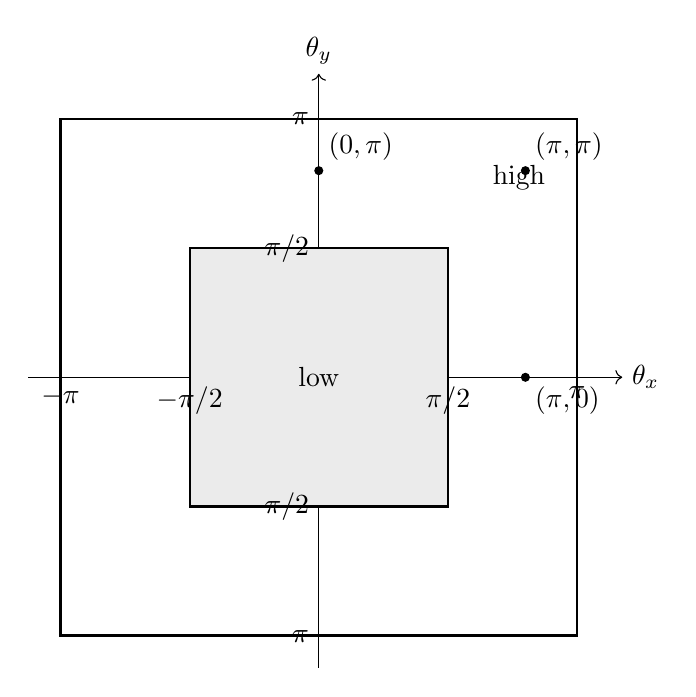
\begin{tikzpicture}[scale=0.82]
  \draw[->] (-4.5,0)--(4.7,0) node[right] {$\theta_x$};
  \draw[->] (0,-4.5)--(0,4.7) node[above] {$\theta_y$};
  \draw[thick] (-4,-4) rectangle (4,4);
  \fill[gray!16] (-2,-2) rectangle (2,2);
  \draw[thick] (-2,-2) rectangle (2,2);
  \node at (0,0) {low};
  \node at (3.1,3.1) {high};
  \node[below] at (-4,0) {$-\pi$};
  \node[below] at (-2,0) {$-\pi/2$};
  \node[below] at (2,0) {$\pi/2$};
  \node[below] at (4,0) {$\pi$};
  \node[left] at (0,-4) {$-\pi$};
  \node[left] at (0,-2) {$-\pi/2$};
  \node[left] at (0,2) {$\pi/2$};
  \node[left] at (0,4) {$\pi$};
  \fill (3.2,0) circle (2pt) node[below right] {$(\pi,0)$};
  \fill (0,3.2) circle (2pt) node[above right] {$(0,\pi)$};
  \fill (3.2,3.2) circle (2pt) node[above right] {$(\pi,\pi)$};
\end{tikzpicture}
\caption{二维 全方向粗化 的频率几何。中心方形是 粗网格 可独立表示的 低频 region；其补集都是 高频 模态。高频不是“两个方向都振荡”，而是至少一个方向落在 粗网格 无法解析的频率带。}
\label{fig:lfa-2d-frequency-region}
\end{figure}

在二维 高频 set 上，式~\eqref{eq:lfa-2d-dinv-a}覆盖区间 $[1/2,2]$。因此 point 加权 Jacobi 的高频 minimax 权重为
\begin{equation}
\omega_\star=\frac45,
\qquad
\mu_\star=\frac35.
\label{eq:lfa-2d-jacobi-optimal}
\end{equation}
这说明不能把一维 $\omega=2/3$ 当成与维数无关的常数。

三维 模态 为
\begin{equation}
\varphi_{i,j,k}(\bm\theta)
=e^{\mathrm i(i\theta_x+j\theta_y+k\theta_z)},
\end{equation}
并有
\begin{equation}
\widetilde{D^{-1}A}
=1-\frac13(
\cos\theta_x+\cos\theta_y+\cos\theta_z).
\end{equation}
低频区域变成 $(-\pi/2,\pi/2]^3$，高频 set 是其补集；对应 $\widetilde{D^{-1}A}$ 范围为 $[1/3,2]$，从而
\begin{equation}
\omega_\star=\frac67,
\qquad
\mu_\star=\frac57.
\label{eq:lfa-3d-jacobi-optimal}
\end{equation}

\section{多维谐波子空间与两网格符号}

二维 全方向粗化 时，$x,y$ 两个方向都存在“是否加 $\pi$”的二元选择。对基本低频 $\bm\theta=(\theta_x,\theta_y)$，粗网格 无法区分四个 细网格 谐波：
\begin{equation}
(\theta_x,\theta_y),\quad
(\theta_x+\pi,\theta_y),\quad
(\theta_x,\theta_y+\pi),\quad
(\theta_x+\pi,\theta_y+\pi).
\label{eq:lfa-two-dimensional-harmonics}
\end{equation}
因此 两网格符号 从一维的 $2\times2$ 扩展为四维 谐波子空间 上的 $4\times4$ 矩阵。三维三个方向各有一次二元 混叠 选择，共得到 $2^3=8$ 个 谐波，对应 $8\times8$ 符号。

由\chapref{ch:two-grid}式~\eqref{eq:two_grid_error}，任意维数的 两网格符号 都保持同一乘积结构：
\begin{equation}
\widetilde E_{TG}(\bm\theta)
=
\widetilde S_{\mathrm{post}}^{\nu_2}
\left[
I-\widetilde P
\widetilde A_H^{-1}
\widetilde R
\widetilde A_h
\right]
\widetilde S_{\mathrm{pre}}^{\nu_1}.
\label{eq:lfa-general-two-grid-symbol}
\end{equation}
只是这里的 $\widetilde A_h$、$\widetilde S$ 变成 $2^d\times2^d$ 矩阵，$\widetilde P$ 是 $2^d\times1$ 列，$\widetilde R$ 是 $1\times2^d$ 行，而 $\widetilde A_H$ 仍对应唯一 粗网格谐波。

最终 两网格 收敛因子 定义为
\begin{equation}
\rho_{TG}
=\sup_{\bm\theta\in\Theta_{low}}
\rho\left(\widetilde E_{TG}(\bm\theta)\right).
\label{eq:lfa-general-two-grid-factor}
\end{equation}
因此评价 平滑器 时必须回到完整组合：单独的 平滑因子 很重要，但它不能替代 $R/P$、粗网格算子 与 粗空间 approximation 对最终 $\rho_{TG}$ 的共同影响。

\section{Chebyshev 多项式平滑器}

前面的 符号 分析提供了理解 Chebyshev 平滑器 所需的谱语言。Weighted Jacobi 用一次线性多项式
\begin{equation}
1-\omega\lambda
\end{equation}
压低目标谱区；Chebyshev 平滑器 则构造更高阶多项式，使其在预先估计的高频 特征值 interval 上具有更小的最大幅值。

实现上，它主要由重复 算子应用、vector update 与少量 scalar recurrence 组成，不需要 Gauss--Seidel 那样的 pointwise ordering dependency，因此适合 GPU 与大规模 MPI。代价是需要估计目标谱区，而且一次 平滑 phase 包含多次 算子应用。评价标准仍然是
\begin{equation}
\text{达到目标精度的时间}
=\text{循环s}\times\text{cost per 循环},
\end{equation}
而不是只看某一步理论 放大因子\cite{baker2011smoothers,bergervergiat2021twostage,hypreBoomer2026}。

\section{各向异性与半粗化}

前面的一维完整推导与多维点 Jacobi 分析都依赖一个隐含条件：粗空间与平滑器的分工必须匹配算子的强耦合方向。考虑
\begin{equation}
-\epsilon u_{xx}-u_{yy}=f,
\qquad
0<\epsilon\ll1.
\label{eq:lfa-anisotropic-model}
\end{equation}
在各向同性网格 $h_x=h_y=h$ 上，标准五点离散的符号为
\begin{equation}
\boxed{
\widetilde A_h(\theta_x,\theta_y)
=
\frac4{h^2}
\left[
\epsilon\sin^2\frac{\theta_x}{2}
+
\sin^2\frac{\theta_y}{2}
\right].
}
\label{eq:lfa-anisotropic-symbol}
\end{equation}
对角部分为
\begin{equation}
D=\frac{2(\epsilon+1)}{h^2}I,
\end{equation}
所以
\begin{equation}
\widetilde{D^{-1}A}
=
\frac{2}{
1+\epsilon
}
\left[
\epsilon\sin^2\frac{\theta_x}{2}
+
\sin^2\frac{\theta_y}{2}
\right].
\label{eq:lfa-anisotropic-dinv-a}
\end{equation}

现在取一个对普通全方向粗化而言明显属于高频的误差
\begin{equation}
(\theta_x,\theta_y)=(\pi,0).
\end{equation}
式~\eqref{eq:lfa-anisotropic-dinv-a} 给出
\begin{equation}
\widetilde{D^{-1}A}(\pi,0)
=
\frac{2\epsilon}{1+\epsilon},
\end{equation}
因此加权 Jacobi 的放大因子为
\begin{equation}
\widetilde S_\omega(\pi,0)
=
1-\omega\frac{2\epsilon}{1+\epsilon}
=
1-\Oh(\epsilon).
\label{eq:lfa-anisotropic-bad-mode}
\end{equation}
当 $\epsilon\rightar行0$ 时，这个在 $x$ 方向剧烈振荡的模态几乎完全不被点平滑器削弱。于是“高频就一定容易平滑”的直觉失效：真正决定平滑难度的是\textbf{离散算子看到的能量尺度}，而不是单看几何频率。

\begin{figure}[htbp]
\centering
\begin{tikzpicture}[x=1.0cm,y=1.0cm,font=\small,>=Stealth]
  \draw[->] (-3.5,0)--(3.7,0) node[right] {$\theta_x$};
  \draw[->] (0,-3.5)--(0,3.7) node[above] {$\theta_y$};
  \draw[thick] (-3,-3) rectangle (3,3);
  \fill[black!8] (-1.5,-1.5) rectangle (1.5,1.5);
  \draw (-1.5,-1.5) rectangle (1.5,1.5);
  \fill (3,0) circle (2.4pt);
  \node[above right] at (3,0) {$(\pi,0)$};
  \draw[->,line width=0.8pt] (2.6,1.0)--(3.0,0.2);
  \node[align=center,font=\scriptsize] at (1.6,1.65)
  {几何上是高频\\但当 $\epsilon\ll1$ 时\\点 Jacobi 几乎不衰减};
\end{tikzpicture}
\caption{强各向异性下的困难模态。频率位置本身不足以判断平滑效果，还必须结合算子符号的方向权重。}
\label{fig:lfa-anisotropic-difficult-mode}
\end{figure}

这也解释了常见补救策略。沿强耦合方向使用线平滑器或面平滑器，相当于在一次平滑中联合处理一整组强耦合自由度；半粗化则避免过早删除平滑器难以处理方向上的分辨率。例如只沿 $y$ 方向粗化：
\begin{equation}
(h_x,h_y)\rightar行(h_x,2h_y).
\end{equation}
此时 $x$ 方向仍保持细分辨率，粗空间不必立即用低分辨率去表示式~\eqref{eq:lfa-anisotropic-bad-mode} 这类困难误差。

从数值角度，这改变了谐波子空间与粗空间逼近性质；从并行角度，它还让问题规模下降更慢。三维只粗化两个方向时，每层自由度数约降为原来的 $1/4$ 而不是 $1/8$，因此总算术工作增加，却能在粗层保留更多并行度。这里数值鲁棒性与硬件并行度可能同时受益，但具体取舍最终仍要用真实达到目标精度的时间验证。

\section{本章小结}

本章首先用 Fourier 符号定量解释 加权 Jacobi 的 平滑性质，然后把 $2h$ 粗化 引起的 混叠 写成 谐波对。对一维 Poisson、全加权、linear 延拓、Galerkin 粗网格算子 以及 一次预平滑/一次后平滑 加权 Jacobi，我们完整构造了
\begin{equation}
2\times2\text{ 两网格符号}
\end{equation}
并得到 $\omega=2/3$ 时
\begin{equation}
\rho_{TG}=\frac19.
\end{equation}
这个结果把“平滑器压高频”和“粗层 校正 去低频”从直觉变成了一个可逐项检查的矩阵计算。

多维情形的核心变化发生在频率空间：二维 低频 region 是中心方形，全方向粗化 产生四个 发生混叠的谐波；三维则产生八个。于是 两网格符号 分别变成 $4\times4$ 与 $8\times8$ 矩阵，但其结构仍由 平滑器、传递算子、粗网格算子 与 细网格算子 的乘积决定。

LFA 的价值是机制分析和参数筛选。物理边界、AMR interface、强变系数和不规则几何会破坏其理想假设，因此最终仍要回到真实离散系统的 残差 history、收敛因子 与 达到目标精度的时间 做验证。

\section*{习题}

\subsection*{Fourier 分析与两网格推导}
\begin{enumerate}[label=\arabic*.]
\item 从 $\varphi_j(\theta)=e^{\mathrm i j\theta}$ 出发，逐步计算一维 Poisson 离散模板 的 Fourier 符号~\eqref{eq:lfa-poisson-1d-symbol}。

\item 对 加权 Jacobi，计算式~\eqref{eq:lfa-wj-one-dimensional-symbol}在 $\theta=\pi/4,\pi/2,3\pi/4,\pi$ 以及 $\omega=1/2,2/3,1$ 时的 放大因子。

\item 取 $\theta=\pi/3$，逐项计算 $\alpha,\beta,s_0,s_1$、$\widetilde C_h^{(2)}$ 与 $\widetilde E_{TG}^{(2)}$，直接验证 一次预平滑/一次后平滑、$\omega=2/3$ 时非零特征值 为 $1/9$。

\item 保持其余设置不变，分别取 $\omega=1/2$ 与 $\omega=3/4$，用式~\eqref{eq:lfa-two-grid-nonzero-eigenvalue}计算 $\theta=\pi/6,\pi/4,\pi/3$ 的 两网格 nonzero 特征值。

\item 推导二维五点 Poisson 的 $\widetilde A(\theta_x,\theta_y)$ 与 $\widetilde{D^{-1}A}$，并计算 模态 $(\pi,0)$、$(\pi,\pi)$、$(\pi/2,\pi/2)$ 的数值。

\item 对二维 基本频率 $(\theta_x,\theta_y)=(\pi/4,\pi/6)$，列出式~\eqref{eq:lfa-two-dimensional-harmonics}中的四个 发生混叠的谐波，并把每个 frequency 分量映射回 $[-\pi,\pi)$。

\item 证明在无限/周期均匀网格上，任意常系数有限 离散模板 的 Fourier 模态 是特征函数，并写出一般 符号 为 离散模板 coefficients 的离散 Fourier transform。

\item 从 全加权 与 线性插值 的空间公式独立推导式~\eqref{eq:lfa-pair-restriction}和~\eqref{eq:lfa-pair-prolongation}，不要直接引用正文结果。

\item 从式~\eqref{eq:lfa-pair-fine-operator}--\eqref{eq:lfa-pair-prolongation}重新推导 粗层 校正 矩阵~\eqref{eq:lfa-coarse-correction-matrix}，并证明其 特征值 为 $0$ 与 $1$。

\item 从式~\eqref{eq:lfa-two-grid-nonzero-eigenvalue}证明 一次预平滑/一次后平滑 两网格 的最优 Jacobi weight 是 $2/3$，最优 收敛因子 是 $1/9$。

\item 若只做一次 pre-平滑 而不做 post-平滑，重新构造 $\widetilde E_{TG}^{(2)}$ 并求其非零特征值。比较它与 symmetric 一次预平滑/一次后平滑 组合的差异。

\item 解释为什么二维 全方向粗化 会得到 $2^2=4$ 个 谐波，而三维得到 $2^3=8$ 个。把论证写成每个坐标方向独立 混叠 的 tensor-product 结构。
\end{enumerate}

\subsection*{符号与数值核验}
\begin{enumerate}[label=\arabic*.]
\item 编程扫描 $\theta\in(-\pi/2,\pi/2]$ 与若干 $\omega$，直接组装式~\eqref{eq:lfa-two-grid-matrix-1d}并计算 谱半径。确认 $\omega=2/3$ 时曲线在非零基本频率上恒为 $1/9$。

\item 同时画出 加权 Jacobi 的 高频 平滑因子 curve 与完整 两网格 convergence-因子 curve，比较“只优化 平滑器”与“优化完整 循环”的区别。

\item 对二维五点 Poisson 绘制 $|\widetilde S_\omega(\theta_x,\theta_y)|$ 的二维图，并在图上叠加式~\eqref{eq:lfa-2d-low-region}的 低频 square。

\item 构造 small periodic Poisson 矩阵，数值求其 Jacobi eigenvectors/特征值，与 Fourier 解析结果逐一匹配；再构造 两网格 iteration 矩阵，与 LFA 的 $1/9$ asymptotic 因子 比较。

\item 将 LFA 预测与有限 Dirichlet grid 上的实测 两网格 因子 比较。随着 grid re细层ment 增大，观察 interior-dominated asymptotic 因子 是否趋近 LFA 预测，并解释 finite boundary effect。
\end{enumerate}

\subsection*{适用边界与迁移}
\begin{enumerate}[label=\arabic*.]
\item 一个 平滑器 的 LFA 平滑因子 更小，但每 sweep 成本高 $60\%$。设计最小 基准测试，使比较对象从“每 sweep 收敛强弱”转为固定 tolerance 下的 达到目标精度的时间。

\item 对强各向异性算子，利用 frequency 符号 判断哪类 模态 难以被 point 平滑器 抑制，并据此说明 line 平滑器、plane 平滑器 或 半粗化 应如何选择方向。

\item LFA 给出一个 传递算子/平滑器 组合的理想 两网格 因子 很小，但真实 AMR 基准测试 收敛明显变差。按“边界、系数跳变、粗细接口、非平移不变 离散模板、并行实现”设计排查顺序，并说明哪些现象属于 LFA 假设外问题。
\end{enumerate}


\part{并行算法与异构执行}
\chapter{并行计算的基本模型}
\label{ch:parallel-model}

\begin{keybox}
\textbf{本章先建立与 OpenMP、CUDA、MPI 无关的并行心智模型。}一个数值算法能否并行，不由 API 决定，而由任务之间的依赖、数据归属、读写集合与同步关系决定。本章只回答“怎样分析一个算法的并行结构”；具体硬件映射从\chapref{ch:mg-parallel-operations}之后开始。
\end{keybox}

\section{任务、数据与依赖}

考虑一个串行程序。把它写成一串语句并不能直接告诉我们哪里可以并行；更有用的表示是把计算拆成若干\textbf{逻辑任务（task）}。每个 task 具有读集合 $R_t$、写集合 $W_t$ 和计算规则。如果两个任务之间不存在必须保持先后顺序的数据依赖，它们原则上就可以并发执行。

最基本的依赖来自同一数据位置的冲突：
\begin{itemize}
\item read--read：两个任务都只读同一数据，不产生顺序约束；
\item write--read：后一个任务需要前一个任务刚写出的结果，必须保持顺序；
\item write--write：两个任务会写同一位置，需要确定唯一顺序或改写算法；
\item reduction：多个任务产生局部贡献，最后需要按结合规则合并。
\end{itemize}

把 task 作为节点、必须满足的先后依赖作为有向边，就得到\textbf{依赖 DAG（directed acyclic graph）}。并行算法的第一步不是“创建多少线程”，而是先确定这张 DAG。

\begin{equation}
\boxed{
\text{算法}
\rightarrow
\text{task}
\rightarrow
(R_t,W_t)
\rightarrow
\text{dependency DAG}
\rightarrow
\text{可并行集合}
}
\label{eq:parallel-analysis-chain}
\end{equation}

例如向量更新
\begin{equation}
y_i\leftarrow a x_i+y_i
\end{equation}
中，第 $i$ 个 task 只读 $x_i,y_i$ 并写 $y_i$；不同 $i$ 的写集合互不相交，所以所有元素更新可以并行。相反，前缀和
\begin{equation}
y_i=y_{i-1}+x_i
\end{equation}
按最直接写法存在链式依赖，不能通过“给每个 $i$ 一个线程”消除依赖。

\section{Work、Span 与可用并行度}

并行复杂度需要同时描述“总共做多少工作”和“最短依赖链有多长”。记
\begin{equation}
W=\text{所有 task 工作量之和},
\qquad
S=\text{依赖 DAG 上的关键路径工作量}.
\end{equation}
$W$ 常称 work，$S$ 常称 span 或 critical-path length。即使拥有无限多处理单元，执行时间也不可能短于 $S$；因此算法自身提供的平均并行度为
\begin{equation}
\boxed{
\mathcal P=\frac{W}{S}.
}
\label{eq:parallel-average-parallelism}
\end{equation}
如果硬件有 $P$ 个执行单元，理想时间至少满足
\begin{equation}
T_P\ge\max\left(\frac{W}{P},S\right).
\label{eq:parallel-lower-bound}
\end{equation}
这条式子解释了一个后面反复出现的现象：当问题规模变小、task 数下降以后，即使每个 task 本身仍然很快，span 不再能被更多硬件隐藏，并行效率也会下降。

Amdahl 定律是同一思想的另一种表达。若总时间中比例 $s$ 必须串行，其他部分可以无限并行，则最大加速比满足
\begin{equation}
S_{\max}=\frac1s.
\end{equation}
它不是说“并行没有意义”，而是提醒我们：固定同步、串行粗层和全局归约都会在规模变大时成为硬上限。

\section{工作分解与数据分解}

把 task 识别出来以后，还必须决定它们如何分配到执行单元。这里有两种相关但不同的分解。

\subsection{工作分解}

工作分解回答“哪个执行单元负责哪些 task”。最细可以一 task 一执行单元，最粗可以一个大块由单个执行单元完成。粒度太细会增加调度和同步成本；粒度太粗则会降低并行度并放大负载不均。

\subsection{数据分解与所有权}

数据分解回答“哪个执行单元拥有或主要负责哪部分数据”。对网格算法，常见做法是按连续空间子区域切分。无论底层是线程、GPU block 还是 MPI rank，都可以先用一个抽象所有权映射表示：
\begin{equation}
\operatorname{owner}(i)=p,
\end{equation}
表示数据项 $i$ 由执行单元 $p$ 负责写回最终结果。

\textbf{所有权首先是一条写入规则。}只要每个输出位置有唯一 owner，就可以避免 write--write 冲突；读取则可能跨越所有权边界。共享内存中跨边界读取仍然是普通 load，分布式内存中则需要通信。这个差别会在\chapref{ch:shared-memory}与\chapref{ch:mpi}分别具体化。

\section{基本并行计算模式}

数值程序中的许多 kernel 可以归入少数稳定模式。认识模式比记住某个 API 更可迁移。

\subsection{Map 与 Stencil}

Map 的典型形式是
\begin{equation}
y_i=F(x_i),
\end{equation}
每个输出只依赖同位置输入。Stencil 则允许读取一个局部邻域：
\begin{equation}
y_i=F\bigl(\{x_j:j\in\mathcal N(i)\}\bigr).
\end{equation}
只要所有 task 写不同 $y_i$，stencil 仍然可以并行；但它比 map 更依赖数据局部性，并在数据分区边界产生额外读取需求。

\subsection{Gather、Scatter 与 Reduction}

Gather 由一个输出 task 主动读取多个输入：
\begin{equation}
y_i=\sum_{j\in\mathcal S(i)}w_{ij}x_j.
\end{equation}
如果每个 $y_i$ 只有一个 writer，通常没有写冲突。Scatter 则由一个输入 task 向多个输出贡献：
\begin{equation}
y_j\mathrel{+}=g_{ij}x_i,
\end{equation}
多个输入可能同时更新同一个 $y_j$，因此需要原子操作、分段累加或重新组织成 gather。

Reduction 把很多局部值合并成少量全局值，例如
\begin{equation}
\|r\|_2^2=\sum_i r_i^2.
\end{equation}
它具有大量局部并行工作，但最终必须沿 reduction tree 合并，因而具有非零 span；在分布式系统中还会变成全局通信。

\section{同步、通信与局部性}

如果某一批 task 的输出是下一批 task 的输入，就需要建立阶段边界。共享内存中这通常表现为 barrier、lock、atomic 或 task dependency；分布式内存中则表现为 point-to-point message 或 collective communication。

通信成本常用最小的 $\alpha$--$\beta$ 模型表示：
\begin{equation}
T_{\mathrm{msg}}\approx\alpha+\beta m,
\label{eq:parallel-alpha-beta}
\end{equation}
其中 $\alpha$ 是启动延迟，$m$ 是消息字节数，$\beta$ 是每字节传输时间。小消息常被 $\alpha$ 主导，大消息更接近带宽项 $\beta m$。

即使没有跨节点通信，数据位置也会影响速度。缓存层次、NUMA、GPU global/shared memory 都说明同一个规律：\textbf{并行度不是唯一目标，任务还应尽量重复使用靠近自己的数据。}因此划分必须同时考虑负载均衡和 locality。

\section{性能成本的统一分解}

对一个并行阶段，可以先用概念模型
\begin{equation}
\boxed{
T\approx T_{\mathrm{compute}}
+T_{\mathrm{memory}}
+T_{\mathrm{sync}}
+T_{\mathrm{comm}}
+T_{\mathrm{launch/schedule}}.
}
\label{eq:parallel-cost-decomposition}
\end{equation}
这不是要求五项严格相加而没有重叠，而是用于诊断“时间主要受哪一类资源约束”。

对内存密集 kernel，算术强度
\begin{equation}
I=\frac{\text{FLOPs}}{\text{bytes transferred}}
\end{equation}
可以与硬件峰值计算率 $F_{\max}$ 和内存带宽 $B_{\max}$ 组成 Roofline 上界：
\begin{equation}
P\le\min(F_{\max},I B_{\max}).
\label{eq:parallel-roofline}
\end{equation}
但 Roofline 只覆盖 compute/memory 竞争；它不能替代 barrier、kernel launch、MPI latency 和全局 reduction 的分析。

\section{并行模型与硬件实现的分离}

到这里仍然没有指定线程、warp 或 rank。统一模型只包含 task、数据、依赖、所有权与通信。后续硬件只是把这些抽象对象映射到不同执行机制：
\begin{center}
\small
\begin{tabularx}{0.96\textwidth}{>{\bfseries}p{2.6cm}XXX}
\toprule
抽象对象 & 共享内存 & GPU & 分布式内存\\
\midrule
task & loop chunk / task & thread / block & rank-local loop\\
数据所有权 & shared array + 写区间 & device array + thread/block mapping & owned subdomain\\
跨边界读取 & 普通共享 load & global/shared-memory load & ghost/halo communication\\
阶段同步 & barrier/task dependency & kernel boundary / device sync & message completion / collective\\
reduction & thread tree reduction & block/device reduction & local reduction + global collective\\
\bottomrule
\end{tabularx}
\end{center}
\chapref{ch:mg-parallel-operations}将先把多重网格每个操作放进这套抽象模型，再从\chapref{ch:shared-memory}开始具体映射到硬件。

\section{本章小结}

并行算法的第一性对象不是 API，而是 task、读写集合、依赖 DAG、工作量、关键路径和数据所有权。Map、stencil、gather/scatter、reduction 与 communication 是后面反复出现的基本模式。硬件优化的本质，是在不破坏依赖与所有权语义的前提下，提高可用并行度、改善 locality，并降低同步与通信固定成本。

\section*{习题}

\subsection*{计算题}
\begin{enumerate}[label=\arabic*.]
\item 一个 DAG 有 64 个单位工作 task，关键路径长度为 8。计算 $W,S,W/S$，并分别给出 $P=4,8,32$ 时由式~\eqref{eq:parallel-lower-bound}得到的时间下界。
\item 某程序串行比例为 $s=0.04$。计算无限并行度下的 Amdahl 加速上限，并计算 $P=8,32,128$ 时理想并行部分完全线性缩放下的加速比。
\item 用 $T=\alpha+\beta m$，取 $\alpha=2\,\mu s$、带宽 $1/\beta=20\,\mathrm{GB/s}$，计算 $m=1\,\mathrm{KB},1\,\mathrm{MB},100\,\mathrm{MB}$ 的消息时间，并判断各自更受 latency 还是 bandwidth 主导。
\item 一个 kernel 每个元素做 18 FLOPs，主存实际读写 64 B。计算 arithmetic intensity；若内存带宽为 $200\,\mathrm{GB/s}$、峰值算力为 $4\,\mathrm{TFLOP/s}$，求 Roofline 上界。
\end{enumerate}

\subsection*{推导与证明题}
\begin{enumerate}[label=\arabic*.]
\item 证明任何调度都必须满足 $T_P\ge W/P$ 与 $T_P\ge S$，从而得到式~\eqref{eq:parallel-lower-bound}。
\item 证明若每个输出位置具有唯一 writer，且所有输入在阶段开始前已经就绪，则纯 gather kernel 不需要为输出写入设置互斥锁。
\item 对二叉 reduction tree 推导 $N$ 个输入的 work 与 span，并与串行 reduction 比较。
\item 给出一个 scatter kernel 存在 write--write race 的具体例子，并证明把它改写成等价 gather 可以消除该 race。
\end{enumerate}

\subsection*{编程与上机题}
\begin{enumerate}[label=\arabic*.]
\item 实现 map、stencil 和 reduction 三个最小 kernel，记录它们的读写集合并画出 dependency DAG。
\item 为一维三点 stencil 实现两种分块粒度，测量单线程和多线程的内存带宽与调度开销。
\item 实现 tree reduction 与串行 reduction，比较不同数组长度下的临界规模。
\item 使用 profiler 或硬件计数器测一个低算术强度 kernel，比较实测带宽与 Roofline 预测。
\end{enumerate}

\subsection*{工程与综合题}
\begin{enumerate}[label=\arabic*.]
\item 给定一个新数值 kernel，设计一张检查表：task 是什么、读写什么、谁拥有输出、是否需要 barrier/reduction/communication、怎样判断粒度是否过细。
\item 某优化把 FLOPs 降低 30\%，却使内存流量增加 2 倍。用 Roofline 与式~\eqref{eq:parallel-cost-decomposition}讨论它可能在哪些机器上更慢。
\item 比较“按数据块固定 owner”和“动态抢 task”两种调度在 locality 与 load balance 上的取舍。
\end{enumerate}

\chapter{多重网格操作的并行结构}
\label{ch:mg-parallel-operations}

\begin{keybox}
\textbf{本章把\chapref{ch:parallel-model}的抽象模型具体化到多重网格。}对每一个 smoother、算子应用、残差、restriction、prolongation、correction、norm 与 ghost fill，都沿着同一条链分析：
\begin{equation}
\boxed{
\text{数值语义}
\rightarrow
\text{状态版本}
\rightarrow
\text{logical task}
\rightarrow
\text{依赖 DAG}
\rightarrow
\text{所有权与粒度}
\rightarrow
\text{同步/通信来源}.
}
\label{eq:mg-parallel-analysis-chain}
\end{equation}
本章仍不选择 OpenMP、CUDA 或 MPI。目标是先回答一个更基础的问题：\textbf{V-cycle 中究竟哪些依赖是数学上必须存在的，哪些依赖只是某种存储或执行方式引入的，以及粗化为什么会系统性地耗尽并行度。}
\end{keybox}

\section{一个 MG Level 上究竟有哪些状态}

对线性多重网格的第 $\ell$ 层，最基本的逻辑对象可以写成
\begin{equation}
\boxed{
u_\ell,\quad
b_\ell,\quad
r_\ell,\quad
e_\ell,\quad
A_\ell,\quad
\text{geometry/coefficient data}.
}
\label{eq:mg-parallel-level-data}
\end{equation}
其中 $u_\ell$ 是当前近似，$b_\ell$ 是当前层右端，
\begin{equation}
r_\ell=b_\ell-A_\ell u_\ell
\end{equation}
是残差，$e_\ell$ 表示误差修正。若采用无矩阵算子，$A_\ell$ 不必以 CSR 等显式稀疏矩阵形式存储，但应用 $A_\ell$ 所需的 stencil、面系数、几何信息与边界元数据仍必须存在。

并行分析时，仅列出这些数组还不够。真正决定依赖的是\textbf{状态版本}。例如一次 Jacobi sweep 中，
\begin{equation}
u_\ell^{(k)}
\longrightarrow
u_\ell^{(k+1)}
\end{equation}
是两个不同的逻辑状态；即使实现时通过 ping-pong buffer 复用物理内存，也不能把二者在依赖图中混成同一个对象。相反，Gauss--Seidel 会在同一个 sweep 内逐步产生并立即消费新状态，因此其 DAG 与 Jacobi 根本不同。

这给出本章第一个重要区分：
\begin{equation}
\boxed{
\text{逻辑状态版本}
\neq
\text{物理数组对象}.
}
\label{eq:mg-state-version-vs-storage}
\end{equation}
前者决定算法依赖，后者决定内存占用和可能出现的 WAR/WAW。许多“并行化困难”其实来自把逻辑上不同的版本强行复用到同一块存储。

在结构网格中，状态通常又以 patch、box 或连续子块为存储与调度单位。热点索引可能采用某一方向连续的一维布局，例如三维 $x$ 连续时
\begin{equation}
p(i,j,k)=i+n_x\bigl[(j-1)+n_y(k-1)\bigr].
\end{equation}
布局本身不改变数学 DAG，却决定 task 聚合以后是否具有良好的 cache line、SIMD 或 coalesced memory access。

\section{把第七章模型落到 MG 操作}

对后面的每一个操作，不再重新发明一套问题，而是直接使用\chapref{ch:parallel-model}的分析流程。最核心的六步可以压缩为：

\begin{enumerate}
\item 写清楚这一操作要产生的\textbf{新状态}；
\item 选择最小有意义的 logical task，并写出 $R_t,W_t$；
\item 判断 RAW 真依赖在哪里，哪些 WAR/WAW 只是原地存储引入；
\item 判断 task 能否重写成 unique-writer 的 gather 形式；
\item 决定实际调度粒度是 point、line、tile、patch 还是更大的 block；
\item 找出必须等待的数据 readiness：本地阶段完成、ghost 就绪、coarse state 就绪或 global reduction 完成。
\end{enumerate}

这样分析以后，OpenMP barrier、GPU kernel boundary、MPI halo 或 collective 都只是同一条依赖边在不同机器上的物理实现，而不是彼此无关的“特殊技巧”。

\section{平滑器首先改变依赖图}

\subsection{Jacobi 的并行性来自状态分离}

Weighted Jacobi 的完整更新是
\begin{equation}
u_i^{(k+1)}
=
u_i^{(k)}
+
\omega D_{ii}^{-1}
\left(
b_i-(Au^{(k)})_i
\right).
\label{eq:mg-parallel-jacobi-full}
\end{equation}
一个 logical task 负责一个新输出 $u_i^{(k+1)}$。它只读取旧状态 $u^{(k)}$ 的 stencil 邻域、$b_i$ 与系数，写入自己的新状态：
\begin{equation}
R_i=
\{u_j^{(k)}:j\in\mathcal N(i)\}
\cup
\{b_i,\text{coefficients}\},
\qquad
W_i=\{u_i^{(k+1)}\}.
\label{eq:mg-jacobi-rw}
\end{equation}
不同 task 可以共享旧输入，却没有输出写冲突，因此同一 sweep 的 point tasks 在算法层面完全独立。

这里有两种实现语义必须分清。若先显式计算
\begin{equation}
r^{(k)}=b-Au^{(k)},
\end{equation}
再做
\begin{equation}
u^{(k+1)}=u^{(k)}+\omega D^{-1}r^{(k)},
\end{equation}
则 residual 是 stencil gather，update 是 map，中间存在 $r^{(k)}$ readiness。若把二者融合，单个 task 直接按式~\eqref{eq:mg-parallel-jacobi-full}产生 $u_i^{(k+1)}$，可以省去一遍 residual 数组的写入与读取，但会改变数据生命周期和 kernel 粒度。

Jacobi 容易并行的根本原因不是“公式简单”，而是
\begin{equation}
\boxed{
u^{(k)}\ \text{在整个 sweep 内只读},
\qquad
u^{(k+1)}\ \text{唯一写入}.
}
\end{equation}
double buffering 把原本可能由原地复用产生的 WAR/WAW 去掉了。

\subsection{Gauss--Seidel 的并行障碍来自新值立即可见}

Lexicographic Gauss--Seidel 在更新 $u_i$ 时会读取本 sweep 已经产生的某些 $u_j^{(k+1)}$。因此其依赖不是存储偶然造成的，而是更新规则本身要求“新值立即进入后续计算”。在最直接排序下，DAG 会出现沿网格传播的长链。

对于标准二维五点或三维七点 Cartesian stencil，耦合图是二分图，可以采用 red--black Gauss--Seidel。一个 sweep 变成
\begin{equation}
\boxed{
\text{all red}
\rightarrow
\text{red state ready}
\rightarrow
\text{all black}
\rightarrow
\text{black state ready}.
}
\label{eq:mg-rbgs-dag}
\end{equation}
同色内部 task 可并行，不同颜色之间存在 RAW 真依赖。

需要保留这个条件的边界：\textbf{“两色即可”来自 stencil 耦合图的二分性，而不是 Gauss--Seidel 的普遍性质。}若离散产生对角耦合、非结构邻接或 block coupling，可能需要更多颜色，或者改用 block/line smoother。颜色数增加会同时增加并行阶段数和同步次数。

\subsection{Line 与 Block Smoother 改变的是 task 粒度}

各向异性问题常使用 line smoother 或 block smoother。此时一个 logical task 不再是单点，而可能是“一条线上的小线性系统”或“一个 block 内的局部求解”。

这类方法常以更多 task 内部 work 换取更强的平滑效果：
\begin{equation}
\text{larger local solve}
\quad\Longleftrightarrow\quad
\text{fewer, heavier tasks}.
\end{equation}
因此不能只比较“每 sweep 的并行度”。真正需要比较的是
\begin{equation}
\boxed{
\text{time per sweep}
\times
\text{sweeps/cycles required for target convergence}.
}
\end{equation}
算法收敛性与并行粒度在 smoother 上第一次直接耦合起来。

\section{算子应用与残差是典型 Stencil Gather}

残差定义为
\begin{equation}
r_i=b_i-(Au)_i.
\end{equation}
对显式 stencil 或无矩阵 operator apply，一个 logical task 负责一个 $r_i$，读取 $u$ 的邻域并只写自己的输出，因此
\begin{equation}
R_i=
\{u_j:j\in\mathcal N(i)\}
\cup
\{b_i,\text{operator data}\},
\qquad
W_i=\{r_i\}.
\end{equation}
这是标准的 unique-writer stencil gather。

如果整个所需邻域都在当前地址空间内，邻域读取只是普通 load；如果某些邻居由别的 rank 拥有，那么\textbf{同一个逻辑 task 并没有改变}，只是它的输入 readiness 需要 halo exchange 保证。可以把任务集合分为
\begin{equation}
\mathcal T
=
\mathcal T_{\mathrm{interior}}
\cup
\mathcal T_{\mathrm{boundary}},
\end{equation}
其中 interior task 的输入全部本地就绪，而 boundary task 还等待 ghost。这个分解是后面 MPI communication overlap 的算法来源，而不是 MPI API 自己创造出来的结构。

物理边界又是另一件事。边界 residual task 仍然产生同一个 $r_i$，只是算子行要使用\chapref{ch:discretization}推导的 Dirichlet、Neumann、Robin 或其他边界闭合。必须区分
\begin{equation}
\boxed{
\text{physical boundary condition}
\neq
\text{partition-boundary data readiness}.
}
\end{equation}

\section{Restriction 与 Prolongation 的关键是输出所有权}

\subsection{Restriction 作为 Coarse-Output Gather}

设 restriction 写成
\begin{equation}
b_H(I)
=
\sum_{j\in\mathcal S(I)}
w_{Ij}r_h(j).
\label{eq:mg-restriction-gather}
\end{equation}
令一个 coarse task 负责一个 $b_H(I)$，则输入是若干 fine residual，输出只有自己的 coarse cell。于是
\begin{equation}
W_I=\{b_H(I)\},
\end{equation}
天然满足 unique writer。

二维 full-weighting 一个 coarse output 最多读取 $3\times3$ 邻域，三维 tensor-product 形式最多读取 $3^3$ 个 fine values。这里维数提升影响的是\textbf{每 task 输入 footprint 与数据复用}，而不是 restriction 是否可并行。

如果 fine/coarse ownership 跨 rank 改变，restriction 还会附带 redistribution，但这是\textbf{输出所有权变化}引起的数据移动，不应与局部 restriction 数值公式混成一个概念。

\subsection{Prolongation 优先采用 Fine-Output Gather}

若按 coarse point 向多个 fine points scatter，
\begin{equation}
e_h(i)\mathrel{+}=p_{iI}e_H(I),
\end{equation}
多个 coarse tasks 可能同时贡献到同一个 fine output，从而形成 WAW 冲突。

更适合大规模并行的语义通常是让每个 fine task 主动 gather：
\begin{equation}
e_h(i)
=
\sum_{I\in\mathcal C(i)}
p_{iI}e_H(I).
\label{eq:mg-prolongation-gather}
\end{equation}
这样每个 fine output 仍然只有一个 writer。注意这里改变的是\textbf{计算组织方式}，不是数学上的 prolongation operator $P$。

如果 prolongation 后立即 correction，
\begin{equation}
u_h\leftarrow u_h+Pe_H,
\end{equation}
并且独立的 $e_h$ 不会再被后继操作读取，则可以把式~\eqref{eq:mg-prolongation-gather}直接融合进 correction，避免物化整个 fine correction 向量。这正是\chapref{ch:parallel-model}所说的“保持语义、改写 DAG 与存储”的例子。

\section{Correction、Reduction 与 Ghost Readiness}

Correction
\begin{equation}
u_h(i)\leftarrow u_h(i)+e_h(i)
\end{equation}
本身是纯 map；若 $e_h$ 已经就绪，每个输出可独立更新。若与 prolongation 融合，它则变成“coarse gather + fine map”的单 task。

残差范数
\begin{equation}
\|r\|_2^2=\sum_i r_i^2
\end{equation}
属于 reduction。其局部平方阶段具有 $\Theta(N)$ work 和大量并行度，真正的 span 来自聚合树。在共享内存中它映射为线程/树形归约，在 GPU 中变成 block/device reduction，在 MPI 中还需要 global collective。若 MG 只作为固定次数 preconditioner apply，内部不一定每层都需要 norm；\textbf{为了“监控一下”而增加的全局 norm 可能直接把一个本可局部执行的阶段变成全局同步点。}

Ghost fill 应理解为一个\textbf{readiness 操作}，而不是某种固定通信 API。它的后置条件是：
\begin{equation}
\boxed{
\text{依赖 ghost 的后继 stencil task 可以读取与 owner 一致的输入版本。}
}
\label{eq:mg-ghost-readiness}
\end{equation}
实现可能是：
\begin{itemize}
\item 同一进程内 patch-to-patch copy；
\item 周期边界映射；
\item AMR coarse-to-fine interpolation；
\item MPI halo exchange；
\item 以上几种操作的组合。
\end{itemize}
因此“ghost cell”是存储概念，“ghost readiness”才是 DAG 概念。

\section{V-Cycle 是一个嵌套 DAG}

把一次 V-cycle 简化成一条阶段链是有用的第一近似：
\begin{equation}
\boxed{
\begin{aligned}
&\text{pre-smooth}
\rightarrow
\text{residual}
\rightarrow
\text{restriction}
\rightarrow
\text{coarse cycle/solve}
\\
&\rightarrow
\text{prolongation/correction}
\rightarrow
\text{post-smooth}.
\end{aligned}
}
\label{eq:mg-parallel-vcycle-dag}
\end{equation}
但真正的执行图至少有三层结构：

\begin{enumerate}
\item \textbf{kernel 内部并行}：例如 residual 中大量独立 point/tile tasks；
\item \textbf{patch/box 级并行}：同一 level 上不同空间块可以独立推进到某些局部依赖边界；
\item \textbf{level 间递归关键路径}：fine residual 必须产生 coarse RHS，coarse error 又必须返回以后才能做 fine correction。
\end{enumerate}

第三层非常重要。典型 V-cycle 的 coarse solve 位于从 fine state 到最终 fine correction 的关键路径上，因此不能靠“fine level 有很多线程”隐藏一个完全串行的 coarse solve。多重网格的核心性能矛盾恰恰是：
\begin{equation}
\boxed{
\text{越粗的 level，数值 work 越少，}
\quad
\text{但它越容易成为同步与关键路径问题。}
}
\label{eq:mg-coarse-paradox}
\end{equation}

另一方面，式~\eqref{eq:mg-parallel-vcycle-dag}也不意味着每个阶段都必须有全局 barrier。若两个 patch 的依赖是局部的，某个 patch 的 residual/transfer 可以在它所需数据就绪后继续，而不必等待整个 level 所有 patch 完成。是否值得采用这种更细 DAG，要由 runtime 开销、实现复杂度与可重叠 work 决定。

\section{粗化怎样系统性耗尽并行度}

$d$ 维 full coarsening 下，未知量数近似满足
\begin{equation}
N_{\ell+1}
\approx
\frac{N_\ell}{2^d}.
\label{eq:mg-parallel-coarsening-count}
\end{equation}
若一个局部 kernel 每 unknown 的 work 为常数量级，
\begin{equation}
W_\ell=\Theta(N_\ell),
\end{equation}
那么各层总 work 构成几何级数。例如三维时
\begin{equation}
N_0+N_1+N_2+\cdots
\approx
N_0
\left(
1+\frac18+\frac1{8^2}+\cdots
\right)
=
\frac87 N_0.
\end{equation}
这解释了为什么从纯算术工作量看，增加很多 coarse levels 仍可能保持近线性复杂度。

但\textbf{work 小不等于时间一定小}。设调度时希望每个活跃 worker 至少获得 $g_{\min}$ 个 unknowns，则第 $\ell$ 层最多有
\begin{equation}
P_\ell^{\mathrm{useful}}
\lesssim
\min\left(
P,
\frac{N_\ell}{g_{\min}}
\right)
\label{eq:mg-useful-workers}
\end{equation}
个有意义的并行 worker。三维每粗化一次，$N_\ell$ 约缩小到原来的 $1/8$，可用 worker 数也可能近似按同样比例下降。

于是 coarse-level 时间更适合用
\begin{equation}
T_\ell
\approx
T_{\ell,\mathrm{useful}}
+
T_{\ell,\mathrm{fixed}}
+
T_{\ell,\mathrm{imbalance}}
\end{equation}
理解。$T_{\ell,\mathrm{useful}}$ 随 $N_\ell$ 快速下降，但 barrier、kernel launch、MPI latency、collective latency、调度和 metadata 等 $T_{\ell,\mathrm{fixed}}$ 不会同比例下降。最终会进入
\begin{equation}
\boxed{
T_{\ell,\mathrm{fixed}}
\gtrsim
T_{\ell,\mathrm{useful}}
}
\end{equation}
的区域，这就是 coarse-grid parallelism collapse。

后面的共享内存线程收缩、GPU coarse-kernel 合并、MPI rank consolidation、agglomeration 与 bottom solver 切换，本质上都是在处理式~\eqref{eq:mg-useful-workers}导致的同一个算法事实。

\section{数据生命周期决定 Fusion 与 Buffer Reuse}

MG 会产生多个临时状态，但“数学对象存在”不等于“整个 solve 期间都必须独占一块数组”。可以把每个向量看成具有
\begin{equation}
\text{birth}
\rightarrow
\text{last use}
\rightarrow
\text{storage reusable}
\end{equation}
的生命周期。

典型例子包括：
\begin{itemize}
\item fine residual $r_\ell$ 在 restriction 完成并确认没有后继读取以后可以复用；
\item prolongated correction 若只用于立即更新 $u_\ell$，可以不独立物化；
\item Jacobi 的 $u^{old}$ 与 $u^{new}$ 可以在 sweep 之间交换角色；
\item coarse temporary 在返回 fine level、最后一次 prolongation 完成后可以释放或进入池化复用。
\end{itemize}

Buffer reuse 的正确判定不是“这个数组现在看起来不用了”，而是
\begin{equation}
\boxed{
\text{所有读取该版本的后继 task 都已经完成。}
}
\end{equation}
过早覆盖会制造真正的 RAW/WAR 错误；过度保守则会增加峰值内存和 memory traffic。

Kernel fusion 也遵循同一规则。例如 residual 后立即 restriction 可以在某些局部算法中尝试 producer--consumer fusion，但只有在 coarse output ownership、fine residual 的其他用途和边界数据 readiness 都允许时才成立。\textbf{Fusion 是 DAG 重写，不是简单把两个 for-loop 拼在一起。}

\section{预条件 Krylov 中存在两层同步结构}

若固定 V-cycle 被用作近似逆
\begin{equation}
z=B_{MG}r,
\end{equation}
则它在外层 Krylov 方法中只是一个 preconditioner apply 子图：
\begin{equation}
\boxed{
\text{Krylov operator/dot}
\rightarrow
\underbrace{\text{MG V-cycle}}_{z=B_{MG}r}
\rightarrow
\text{Krylov update/dot}.
}
\label{eq:mg-parallel-preconditioned-krylov-dag}
\end{equation}

这时需要区分两类同步：

\begin{itemize}
\item MG 内部主要来自 stencil readiness、颜色阶段、transfer、coarse recursion 和可能的 coarse redistribution；
\item Krylov 外层还会引入 dot product、norm 等全局 reduction。
\end{itemize}

因此一个 MG kernel 即使局部扩展很好，整个 Krylov solve 仍可能被外层 global reductions 限制。反过来，为了减少 V-cycle 内部同步而改变 smoother，也必须重新检查 preconditioner quality，因为迭代次数可能上升。

如果 $B_{MG}$ 每次 apply 都执行固定 cycle、固定 smoother 和固定粗层策略，可以把它看成固定线性算子。若 inner tolerance、cycle 数或粗层策略随迭代变化，则 preconditioner apply 本身可能变化，需要\secref{sec:mg-preconditioner}中的 flexible Krylov 视角。

\section{维数、边界与分区改变的是成本结构}

对边长约为 $n$ 的 $d$ 维规则子域，内部 work 与体积成正比，
\begin{equation}
W_{\mathrm{interior}}\sim n^d,
\end{equation}
而一层边界/halo 数据与表面积成正比，
\begin{equation}
Q_{\mathrm{boundary}}\sim n^{d-1}.
\end{equation}
因此
\begin{equation}
\frac{Q_{\mathrm{boundary}}}{W_{\mathrm{interior}}}
\sim
\frac1n.
\label{eq:mg-parallel-surface-volume}
\end{equation}
这一个几何关系会在不同硬件上表现成不同成本：
\begin{itemize}
\item CPU tile 边界主要造成 cache/workset 重复与可能的 NUMA 访问；
\item GPU tile/block 边界影响 shared-memory reuse、global-memory traffic 与 occupancy；
\item MPI partition boundary 才真正产生远端消息。
\end{itemize}

还必须区分三种“边界”：
\begin{equation}
\boxed{
\text{physical boundary}
\neq
\text{partition boundary}
\neq
\text{AMR coarse--fine interface}.
}
\label{eq:mg-boundary-classes}
\end{equation}
物理边界改变离散算子；partition boundary 不改变 PDE，只改变输入数据的取得方式；AMR coarse--fine interface 则需要层间插值、平均或通量匹配。三者都可能使用 ghost-like storage，却来自完全不同的数学语义。

\section{MG 操作的统一并行画像}

\begin{center}
\small
\begin{tabularx}{0.99\textwidth}{>{\bfseries}p{2.0cm}p{2.35cm}p{2.65cm}X}
\toprule
操作 & 典型数据流 & 核心状态依赖 & 主要并行风险/成本来源\\
\midrule
Jacobi & stencil gather + map & $u^{(k)}\rightarrow u^{(k+1)}$ & old/new 存储、带宽、sweep boundary\\
GS/RBGS & ordered/colored stencil & 同 sweep 新值被后继读取 & 长依赖链、color barrier、颜色数\\
算子/残差 & stencil gather & 输入版本/ghost ready & bandwidth、boundary readiness\\
restriction & coarse-output gather & fine residual ready & input footprint、ownership redistribution\\
prolongation & fine-output gather & coarse error ready & scatter 冲突、coarse/fine ownership\\
correction & map 或 fused gather & correction ready & memory pass、fusion lifetime\\
norm/dot & reduction & 全部局部贡献 ready & reduction span、global collective\\
ghost fill & copy/interpolate/exchange & owner version $\rightarrow$ ghost version & copy、插值、message latency\\
coarse solve & 依算法而定 & coarse RHS ready & 并行度塌缩、固定开销、bottom solver\\
\bottomrule
\end{tabularx}
\end{center}

这张表不是实现菜单，而是后续硬件章节的共同语义接口。任何 OpenMP、CUDA、MPI 或混合实现都应该能说明自己如何实现这些状态依赖和所有权规则。

\section{从一个新 MG Kernel 到可执行设计}

遇到新的 MG 操作或优化方案，可以按以下顺序判断：

\begin{enumerate}
\item 先写数学输入、输出和状态版本，不看现有循环代码；
\item 选择 point/line/tile/patch 级 logical task，列出 $R_t,W_t$；
\item 判断依赖是 RAW 真依赖，还是由 in-place storage 引入的 WAR/WAW；
\item 尽量寻找 unique-writer gather 表达；
\item 确定哪些 task 只依赖 local/owned 数据，哪些要等 ghost、coarse state 或 reduction；
\item 估算本层 $W_\ell$、可用 task 数和合理的 $P_\ell^{\mathrm{useful}}$；
\item 再估 bytes、temporary lifetime、message volume、barrier/reduction count；
\item 最后才选择线程、GPU 或 rank 映射，并用 profiler 验证瓶颈。
\end{enumerate}

如果某个优化无法在这条链上说明“它究竟改变了 DAG、数据移动、粒度还是固定开销”，那么它通常还没有被充分理解。

\section{本章小结}

多重网格的并行结构不是“把每个 for-loop 加上 parallel”这么简单。Jacobi 的并行性来自 old/new 状态分离；Gauss--Seidel 的障碍来自新值立即可见；restriction/prolongation 的关键是输出所有权；norm/dot 的关键是聚合 span；ghost fill 的本质是建立输入版本 readiness；完整 V-cycle 则是一个带 level recursion 的嵌套 DAG。

粗化同时带来两个方向相反的效果：总算术 work 形成快速收敛的几何级数，但可用 task 数也按 $2^d$ 的因子迅速减少。于是越到粗层，越不是“算得多”，而是“可并行工作不足以摊薄同步、通信与调度固定成本”。后续 CPU、GPU 与 MPI 章节只是把这一统一结构映射到不同机器。

\section*{习题}

\subsection*{状态与依赖推导}
\begin{enumerate}[label=\arabic*.]
\item 对 weighted Jacobi 写出 $u^{(k)}$、$r^{(k)}$、$u^{(k+1)}$ 三种状态之间的 DAG。分别画出“先 residual 后 update”和“fused Jacobi”两种组织，并指出后者消除了哪些中间数据流。
\item 对原地 lexicographic GS 的相邻三个点写出 RAW 依赖；再对标准二维五点 RBGS 画出 red/black 两阶段 DAG。
\item 说明为什么“二维五点 RBGS 可以两色”不能直接推广为“任何 GS 都只需要两色”，并给出一个含对角耦合的 stencil 作为反例。
\item 对 gather restriction 与 scatter prolongation 分别列出 $R_t,W_t$，指出何时会出现 WAW。
\item 把 ghost fill 表述为 producer--consumer 依赖，区分 owner version、ghost version 和后继 boundary stencil task。
\end{enumerate}

\subsection*{Work、并行度与粗层分析}
\begin{enumerate}[label=\arabic*.]
\item 对 $256^3\rightarrow128^3\rightarrow64^3\rightarrow32^3\rightarrow16^3$ 层级，计算每层 unknown 数与相对 finest level 的比例。
\item 证明三维 full coarsening 下 $\sum_\ell N_\ell\le(8/7)N_0$，并解释为什么这个结果不能推出 coarse levels 的 wall time 可以忽略。
\item 设 $P=64$，希望每个活跃 worker 至少处理 $g_{\min}=4096$ 个 unknowns。对上一题各层计算式~\eqref{eq:mg-useful-workers}给出的最大有用 worker 数。
\item 假设每层 useful work time 与 $N_\ell/P_\ell$ 成正比，而每层固定同步成本为 $5\,\mu s$。构造一个简单模型，找出从哪一层开始 fixed cost 超过 useful work。
\item 推导 $d$ 维 full coarsening 下总 work 的几何级数上界，并比较 $d=2$ 与 $d=3$ 的并行度衰减速度。
\end{enumerate}

\subsection*{实现与验证}
\begin{enumerate}[label=\arabic*.]
\item 实现 residual、Jacobi、restriction、prolongation、correction 和 norm 的串行版本，记录每个 kernel 的 FLOPs、读写字节和输出所有权。
\item 实现独立 $e_h$ 数组的 prolongation+correction 与 fused 版本，验证数值一致性并比较 memory traffic。
\item 为三层 V-cycle 记录每个临时向量的 birth、last use 与可复用时刻，设计一套不破坏依赖的 buffer pool。
\item 把 residual task 分成 interior 与 ghost-dependent boundary 两组，在单进程环境中先验证两组任务任意交错执行仍得到相同结果。
\item 对 fixed V-cycle 与“每层都计算 residual norm”的版本比较同步点数量，解释哪些 norm 是算法必需、哪些只是诊断开销。
\end{enumerate}

\subsection*{工程诊断}
\begin{enumerate}[label=\arabic*.]
\item 某 coarse level 只有 12000 unknowns，却仍启动 64 个 CPU threads。按本章模型列出可能的效率损失，并设计 thread shrinking 规则。
\item 某 GPU V-cycle 的 finest residual 已达到很高带宽，但总 solve 仍很慢。只使用本章抽象，列出 coarse-level parallelism、reduction、launch 与 data-lifetime 四条诊断路径。
\item 某 MPI 版本 restriction 后立刻做 rank consolidation。说明需要区分哪些时间属于数值 restriction，哪些属于 ownership redistribution，并给出 break-even 判断所需的测量项。
\item 一个新的 smoother 每 sweep 比 Jacobi 慢 2 倍，但 V-cycle 数减少到原来的 35\%。说明为什么只能用 time-to-solution 而不能用单 sweep 时间判断优劣，并列出还应比较的同步与并行度指标。
\end{enumerate}

\chapter{共享内存多重网格}
\label{ch:shared-memory}

\begin{keybox}
\textbf{共享内存并行的核心并不是“所有线程都能看到同一个数组”，而是把\chapref{ch:mg-parallel-operations}中的状态版本、所有权和依赖映射到一个共享地址空间。}在这类机器上，跨线程读取通常不需要显式消息，但仍然存在三类完全不同的问题：
\begin{equation}
\boxed{
\text{谁写}
\quad+\quad
\text{数据物理上放在哪里}
\quad+\quad
\text{什么时候其他线程可以安全读取}.
}
\label{eq:shared-memory-three-questions}
\end{equation}
因此共享地址空间只消除了“必须通过网络取得远端字节”这一层问题，并没有消除 cache、NUMA、同步、false sharing、调度和带宽瓶颈。
\end{keybox}

\section{共享地址空间不等于统一代价}

设一个 level 上有
\begin{equation}
u[p],\quad b[p],\quad r[p],
\end{equation}
所有线程都可以用普通地址访问这些数组。从编程接口看，它们处在同一个地址空间中；从硬件看，同一个地址可能对应：

\begin{itemize}
\item 当前核心的 L1/L2 cache line；
\item 共享 LLC 中的数据；
\item 本 socket 的本地 DRAM；
\item 另一个 NUMA node 的 DRAM；
\item 刚被其他核心修改、正在通过 cache coherence 协议传播的新版本。
\end{itemize}

因此“共享”只说明\textbf{地址可达}，不说明访问延迟和带宽相同。

把\chapref{ch:parallel-model}的三个概念直接搬过来：

\begin{enumerate}
\item \textbf{逻辑所有权}：哪个线程负责某个输出区域的最终写入；
\item \textbf{物理放置}：相关页面和 cache line 实际位于哪个 NUMA node / cache hierarchy；
\item \textbf{执行分配}：当前这个 tile 由哪个 worker 执行。
\end{enumerate}

一个正确但很慢的共享内存程序，经常不是所有权错了，而是后两者错位了：线程在 socket 1 上执行，却不断读取 first-touch 到 socket 0 的页面。

\section{正确性的第一原则仍然是 Unique Writer}

对 Jacobi、residual、restriction、prolongation 等 gather 型 kernel，最简单可靠的规则仍然是
\begin{equation}
\boxed{
\text{每个输出位置在一个阶段内只有一个 writer}.
}
\label{eq:shared-memory-unique-writer}
\end{equation}

假设 residual task $t_i$ 负责
\begin{equation}
r_i=b_i-(Au)_i.
\end{equation}
它可能读取其他线程输出区域附近的 $u_j$，但只要这一阶段的 $u$ 是只读版本，而 $r_i$ 只有当前 task 写入，就不存在数据竞争。

这说明\textbf{读取越过 tile 边界本身不是 race}。race 的来源是两个并发 task 对同一存储位置至少有一个写访问，并且缺少满足程序语义的同步关系。

共享内存实现还必须考虑\textbf{可见性}。例如 RBGS 的 black phase 必须读取 red phase 已完成的新值；这里不仅逻辑上有 RAW 依赖，还需要实际执行机制保证 red 写入在 black 读取前已经完成并对其可见。OpenMP barrier、task dependency 或其他同步原语承担的正是这个职责。

\section{Logical Task 与线程调度粒度必须分开}

在\chapref{ch:mg-parallel-operations}中，一个 residual logical task 可以只负责一个 cell。但真实 CPU 不会为每个 cell 创建一个独立重量级线程任务。通常会把大量 point tasks 聚合成 tile、chunk 或 box：
\begin{equation}
T
=
n_x^{(t)}
\times
n_y^{(t)}
\times
n_z^{(t)}.
\end{equation}

于是出现两个尺度：

\begin{equation}
\boxed{
\text{point-level dependency analysis}
\quad\neq\quad
\text{tile-level scheduling}.
}
\label{eq:shared-memory-two-granularities}
\end{equation}

前者回答正确性与算法并行度，后者决定 runtime overhead、locality 和 load balance。

tile 太小通常会带来：
\begin{itemize}
\item 调度与任务元数据开销增加；
\item 相邻 tile 重复读取边界 cache lines；
\item 更多线程同时触及相邻内存，增加 coherence traffic；
\item 动态调度时工作窃取或队列操作更频繁。
\end{itemize}

tile 太大则会：
\begin{itemize}
\item 降低可调度 task 数；
\item 放大 patch 间 workload 差异；
\item 使最慢 tile 决定阶段尾部时间；
\item 在 coarse level 上更早出现“task 数小于线程数”。
\end{itemize}

合理粒度必须在 locality、调度开销与负载均衡之间折中。

\section{Stencil Tile 的工作集与边界放大}

对一层 halo 的三维 stencil，若输出 tile 为
\begin{equation}
n_x^{(t)}\times n_y^{(t)}\times n_z^{(t)},
\end{equation}
输入可能需要扩张为
\begin{equation}
(n_x^{(t)}+2)
\times
(n_y^{(t)}+2)
\times
(n_z^{(t)}+2).
\end{equation}
记输出体积为 $V_t$，输入 footprint 为 $V_t^+$，定义
\begin{equation}
\eta_{\mathrm{ws}}
=
\frac{V_t^+}{V_t}.
\label{eq:shared-memory-working-set-amplification}
\end{equation}

$\eta_{\mathrm{ws}}$ 不是“实际 DRAM 流量一定增加这么多倍”，因为邻近 tile 可能从 cache 复用数据；它只是一个几何上的工作集放大指标。它提醒我们：tile 越小，边界相对比例越大，对 locality 的要求越高。

因此 stencil tile 选择不能只看“能放多少线程”，还要看：
\begin{equation}
\boxed{
\text{tile footprint}
\quad\text{是否适合 cache hierarchy}.
}
\end{equation}

\section{False Sharing：没有数据 Race 也可能很慢}

共享内存中一个很典型的反直觉现象是：两个线程写\textbf{不同变量}，程序完全正确，却仍然互相拖慢。

如果这些变量位于同一个 cache line，线程 A 修改 line 中的一部分，线程 B 修改同一 line 的另一部分，cache coherence 仍可能让这条 line 在核心之间反复失效和迁移。这就是 false sharing。

例如每线程 partial sum 若紧密排列为
\begin{equation}
s_0,s_1,\ldots,s_{P-1},
\end{equation}
多个线程可能同时更新同一条 cache line 上的不同 $s_p$。逻辑上每个元素有唯一 writer，却仍产生 coherence traffic。

因此要区分：
\begin{equation}
\boxed{
\text{data race}
\neq
\text{false sharing}.
}
\end{equation}

前者是正确性问题；后者是 cache-line 粒度的数据放置问题。对 thread-private counters、reduction buffers 和边界 metadata，padding 或分块布局有时比继续优化算术指令更重要。

\section{静态与动态调度对应不同代价模型}

对规则均匀网格，一个 tile 的 work 往往近似一致，静态调度通常具有明显优势：
\begin{itemize}
\item 低调度开销；
\item worker 与数据区域关系稳定；
\item 更容易维持 cache/NUMA affinity；
\item 多个 sweep 中可重复使用相同划分。
\end{itemize}

若 patch 大小差异明显、embedded boundary 导致每 cell 工作不一致，或某些 block smoother 代价变化很大，静态划分可能产生严重 tail imbalance。此时 dynamic/guided scheduling 或显式 task queue 可以改善负载平衡，但代价是 locality 和调度开销变差。

可以把阶段时间近似写成
\begin{equation}
T_{\mathrm{stage}}
\approx
\max_p W_p
+
T_{\mathrm{schedule}}
+
T_{\mathrm{memory/coherence}},
\end{equation}
其中 $W_p$ 是 worker $p$ 实际承担的工作时间。动态调度试图降低 $\max_p W_p$，但通常会提高后两项。

因此“dynamic 比 static 更高级”是错误心智模型。它们只是不同 workload 下的不同折中。

\section{Jacobi、Residual 与 Transfer 的线程映射}

\subsection{Jacobi 与 Residual}

Jacobi 与 residual 都是 unique-writer stencil gather。一个常见线程映射是：

\begin{algorithm}[htbp]
\caption{共享内存 tile-based residual}
\begin{algorithmic}[1]
\State 输入 $u,b$ 与 operator data 在本阶段只读，输出为 $r$
\State 将 owned cells 聚合为互不重叠输出 tiles
\ForAll{tiles $T$ \textbf{in parallel}}
  \ForAll{cells $i\in T$}
    \State 读取 $u_i$ 与 stencil neighbors
    \State $r_i\gets b_i-(Au)_i$
  \EndFor
\EndFor
\end{algorithmic}
\end{algorithm}

tile 只规定\textbf{输出写入范围}。读取邻居可以跨越 tile 边界，因为所有线程共享地址空间。这里不需要 halo message；若 patch 数据结构显式保存 ghost，则 ghost copy 是另外一个 producer--consumer 阶段。

Jacobi 若使用 old/new arrays，每个 sweep 结束后只需交换逻辑角色：
\begin{equation}
u^{old}\leftrightarrow u^{new}.
\end{equation}
不要把“交换指针/handle”误解为拷贝整个数组。

\subsection{Restriction 与 Prolongation}

Restriction 采用 coarse-output gather：线程拥有一组 coarse outputs，从 fine residual 读取所需邻域。Prolongation 采用 fine-output gather：线程拥有一组 fine outputs，从 coarse error 读取插值邻域。二者都延续第八章的 unique-writer 规则。

如果 prolongation 之后立即 correction，可以融合为
\begin{equation}
u_h(i)
\mathrel{+}=
\sum_I p_{iI}e_H(I).
\end{equation}
共享内存上的主要收益通常不是减少“线程数”，而是少物化一个 $e_h$ 数组、少一次完整 fine-grid memory pass。是否值得融合应通过 memory traffic 与后继数据生命周期判断。

\section{Gauss--Seidel 把同步直接放进热路径}
\label{sec:shared-rbgs}

Lexicographic GS 的依赖链不适合普通 parallel-for。对于标准五点/七点 stencil，RBGS 把一个 sweep 组织成
\begin{equation}
\text{parallel red}
\rightarrow
\text{barrier}
\rightarrow
\text{parallel black}
\rightarrow
\text{barrier}.
\label{eq:shared-rbgs-barriers}
\end{equation}

每个颜色内部可并行，但颜色之间的 barrier 属于算法真依赖，而不是“OpenMP 太慢”造成的额外步骤。

如果一个 V-cycle 在某层执行 $\nu_1$ 次 pre-smoothing 和 $\nu_2$ 次 post-smoothing，那么仅 RBGS 颜色阶段就会重复出现大量 barrier。随着 coarse level work 下降，
\begin{equation}
T_{\mathrm{barrier}}
\end{equation}
在单 sweep 中的占比会不断上升。

这说明 smoother 选择必须同时比较：
\begin{equation}
\boxed{
\text{convergence per sweep}
\quad\text{与}\quad
\text{parallel cost per sweep}.
}
\end{equation}
一个单 sweep 较慢但显著减少 V-cycle 数的 smoother 仍可能具有更小的 time-to-solution。

\section{Reduction 既有同步成本也有数值语义}

残差范数可以先做线程私有局部和
\begin{equation}
s_p
=
\sum_{i\in\Omega_p}r_i^2,
\end{equation}
再做
\begin{equation}
\|r\|_2
=
\sqrt{\sum_p s_p}.
\end{equation}

相比每个 cell 对单一全局标量做 atomic update，private partial sum + tree reduction 通常具有更好的扩展性。

但这里有三个不同问题：

\begin{enumerate}
\item \textbf{竞争}：避免所有线程写同一标量；
\item \textbf{false sharing}：不同 partial sums 最好避免高频写入同一 cache line；
\item \textbf{reproducibility}：不同 reduction tree 会改变浮点加法顺序，因此末位可能不同。
\end{enumerate}

如果 residual norm 只用于诊断，而不是算法控制条件，则它还是一个可选同步点。对固定-cycle multigrid，减少不必要 norm 往往比优化 norm kernel 本身更有效。

\section{NUMA：共享虚拟地址背后的物理分布}

在多 socket 系统中，程序看到统一虚拟地址空间，但物理页面通常归属于某个 NUMA node。一个常见策略是 first-touch：页面第一次被某个线程写入时，操作系统倾向于把它放在该线程所在 node 的本地内存。

如果所有数组由单线程初始化，
\begin{equation}
u,b,r,e,\text{coefficients}
\end{equation}
可能大量集中在一个 node。随后其他 socket 的线程虽然能直接 load，却会产生 remote memory traffic。

因此初始化本身应该采用与后续计算相近的空间划分：
\begin{equation}
\boxed{
\text{compute ownership}
\approx
\text{initialization ownership}
\approx
\text{NUMA placement}.
}
\label{eq:shared-numa-alignment}
\end{equation}

还需要配合 thread affinity。若 worker 在运行期间频繁跨 socket 迁移，即使 first-touch 最初正确，数据亲和性也会被破坏。

对多重网格尤其要注意：每个 level 都有自己的数组。只给 finest level 做并行 first-touch，而 coarse levels 仍由单线程初始化，会把 NUMA 问题藏到 V-cycle 后半段。

\section{内存带宽决定线程扩展何时饱和}

Poisson 类 stencil 往往具有较低算术强度。随着线程数增加，性能最初可能近似线性提升，直到 socket/NUMA node 的可持续 memory bandwidth 接近饱和。

可以用一个简化模型理解：
\begin{equation}
P_{\mathrm{kernel}}(P)
\le
\min
\left(
P F_{\mathrm{core}},
I B_{\mathrm{socket}}(P)
\right),
\end{equation}
其中 $B_{\mathrm{socket}}(P)$ 随线程增加先上升，随后接近平台带宽上限。

因此当 residual 已经把 memory bandwidth 打满以后，再增加线程可能出现：
\begin{itemize}
\item wall time 几乎不再下降；
\item parallel efficiency 继续恶化；
\item cache/coherence 与 barrier 成本反而增加。
\end{itemize}

这种现象不是“并行度不足”。算法可能仍有海量 point tasks，只是\textbf{机器资源已经从 core 数切换成 memory bandwidth}。

判断两者的方法也不同：并行度不足应看 task 数、$W/S$ 和 worker idle；带宽饱和则应看 memory bandwidth、LLC miss、bytes/s 与 Roofline。

\section{Parallel Region 与 Barrier 也是固定成本}

若每个小 kernel 都反复创建/销毁线程团队，或者频繁进入独立 parallel region，fork/join 与 runtime bookkeeping 可能在 coarse levels 上占明显比例。

一种常见设计是维持较长生命周期的线程团队，在内部通过 worksharing、task dependency 或必要 barrier 推进多个 MG 阶段，而不是每个小 loop 都重新创建执行上下文。

但减少 barrier 不能破坏状态依赖。例如 residual 尚未完全写好时，restriction 不能随意读取未完成区域，除非实现显式 patch/task-level producer--consumer dependency。于是
\begin{equation}
\boxed{
\text{barrier elimination}
\neq
\text{dependency elimination}.
}
\end{equation}
真正能删除的只是比 DAG 要求更强的全局同步。

\section{共享内存 V-Cycle 的执行结构}

把式~\eqref{eq:mg-parallel-vcycle-dag}映射到线程后，一个典型 level 可以理解为：

\begin{enumerate}
\item pre-smooth：线程处理各自 tiles，RBGS 等方法内部可能有颜色 barrier；
\item residual：unique-writer stencil gather；
\item restriction：coarse-output gather；
\item 进入 coarse level，可用 tile 数和 useful worker 数下降；
\item coarse result ready 后做 prolongation/correction；
\item post-smooth；
\item 只有算法需要时才做 residual norm/reduction。
\end{enumerate}

这里没有网络 halo exchange。即使 patch/box 容器显式保存 ghost，单进程内 ghost fill 也通常是 copy、periodic mapping 或 coarse--fine interpolation。它们仍然是 readiness task，却不是 MPI 通信。

如果 runtime 支持细粒度 task dependency，不同 patch 可以在局部数据 ready 后继续推进；如果 runtime overhead 大于可获得的 overlap，则 level-wide worksharing + 少量 barrier 反而更高效。选择取决于 task 粒度与实际 critical path，而不是“异步越多越先进”。

\section{粗网格上的线程收缩}

由式~\eqref{eq:mg-useful-workers}，粗化后有意义的 worker 数会快速下降。共享内存中可以写成
\begin{equation}
P_\ell
\le
\min
\left(
P_{\max},
\frac{N_\ell}{g_{\min}}
\right).
\label{eq:shared-thread-shrinking}
\end{equation}

固定使用全部线程会让每个线程只处理极少 cells，却仍支付：
\begin{itemize}
\item barrier；
\item runtime scheduling；
\item cache line ownership 迁移；
\item reduction fan-in；
\item 可能的 NUMA 远端访问。
\end{itemize}

因此 thread shrinking 的目标不是“少用核心省资源”，而是保持
\begin{equation}
\boxed{
\text{useful work per active worker}
}
\end{equation}
高于固定开销能够接受的阈值。

最粗层还可能切换为单线程、小线程组或直接法。这个切换点应通过 benchmark 决定，而不是固定写成某个 unknown 常数。

\section{共享内存性能诊断顺序}

当一个 OpenMP/线程版 V-cycle scaling 不理想时，建议按以下顺序排查：

\begin{enumerate}
\item \textbf{正确性层}：是否保持 unique writer、状态版本和必要 happens-before；
\item \textbf{并行度层}：当前 level 有多少 tiles，是否已经少于线程数；
\item \textbf{负载层}：各线程 work 是否均衡，尾部是否由少量重 tile 决定；
\item \textbf{带宽层}：memory bandwidth 是否已经饱和；
\item \textbf{cache/coherence 层}：是否有 false sharing、过小 tile、重复边界流量；
\item \textbf{NUMA 层}：页面放置与线程 affinity 是否匹配；
\item \textbf{同步层}：barrier、reduction、parallel region 和 scheduler overhead 占比多少；
\item \textbf{算法层}：smoother 的同步成本是否换来了足够的 convergence improvement。
\end{enumerate}

只有先区分这些层次，\texttt{gomp\_barrier\_wait}、低 CPU utilization 或 bandwidth plateau 才能被解释，而不是简单归结为“OpenMP 不行”。

\section{本章小结}

共享内存并行保留了多重网格的原始算法语义，但把跨所有权数据访问从“消息”变成了共享 load。真正需要管理的是 unique writer、状态可见性、tile 粒度、cache line、NUMA placement、线程调度与同步。

这一章最重要的三个区分是：共享地址空间不等于统一访问代价；无 data race 不等于无 false sharing；高算法并行度不等于线程数可以无限扩展。细层常受 memory bandwidth 限制，粗层则逐渐转向 task scarcity、barrier 与 runtime fixed cost。thread shrinking、persistent parallel region 和 locality-aware tiling 都是在回应这条尺度变化。

\section*{习题}

\subsection*{粒度与工作集}
\begin{enumerate}[label=\arabic*.]
\item 一个 $32^3$ tile 的一层 halo 输入 footprint 为 $34^3$。计算式~\eqref{eq:shared-memory-working-set-amplification}；再比较 $16^3$ 与 $64^3$ tile。
\item 对 $256^3$ 网格使用 32 个线程，连续 full coarsen 三层。计算每层每线程平均 unknown 数，并判断何时开始低于 $g_{\min}=4096$。
\item 设计两种 tile：$64\times4\times4$ 与 $16^3$。在不知道具体 cache 参数时，比较它们在连续访问、表面积/体积比和可调度 task 数上的结构差异。
\item 解释为什么“cell 越小、task 越多”并不推出实际线程并行度越高。
\end{enumerate}

\subsection*{正确性、Cache 与 NUMA}
\begin{enumerate}[label=\arabic*.]
\item 证明 Jacobi old array 只读、新数组 unique writer 时，不需要 tile 间锁；指出 sweep 结束时仍需要什么 readiness 条件。
\item 构造一个两个线程分别更新不同标量但发生 false sharing 的例子，并说明为什么它没有 data race。
\item 设计 per-thread reduction buffer 的 cache-line-friendly 布局，并讨论 padding 带来的内存开销。
\item 在双 socket 系统中比较 serial initialization 与 parallel first-touch，画出“线程、虚拟页、NUMA node”的对应关系。
\item 说明 thread migration 为什么可能破坏已经正确建立的 first-touch locality。
\end{enumerate}

\subsection*{同步与 Smoother}
\begin{enumerate}[label=\arabic*.]
\item RBGS 做 3 次 pre 和 3 次 post sweep，每 sweep 两颜色。计算单 level 至少出现多少个颜色完成点，并区分算法依赖与具体 barrier API。
\item 比较 point Jacobi 与 RBGS：同时报告每 sweep memory traffic、barrier 数、convergence factor 与 time-to-solution。
\item 假设 coarse level useful work 只有 $8\,\mu s$，一次 barrier 为 $2\,\mu s$。估算含 8 次 barrier 的 smoother 中同步占比。
\item 设计一个 patch-level producer--consumer 方案，使部分 residual 完成后即可开始 restriction；说明它需要哪些局部 dependency 才能正确替代 level-wide barrier。
\end{enumerate}

\subsection*{性能实验与诊断}
\begin{enumerate}[label=\arabic*.]
\item 扫描线程数并同时记录 wall time、memory bandwidth、LLC miss 与 barrier wait time，判断 scaling 饱和究竟来自 bandwidth 还是 task scarcity。
\item 比较 static、dynamic 与 guided schedule 在规则网格和高度不均匀 patch workload 上的时间、NUMA locality 与 scheduler overhead。
\item 比较“每个 kernel 独立 parallel region”和“一个 persistent parallel region 内执行整个 V-cycle”的开销。
\item 设计按 MG level 自动选择 active thread 数的策略，输入至少包括 $N_\ell$、tile 数、测得的 barrier cost 与 memory-bandwidth saturation point。
\item 给出一个 \texttt{gomp\_barrier\_wait} 占比很高的 profile，列出至少四种不同根因，并说明下一步分别应观测什么证据。
\end{enumerate}

\chapter{GPU 执行模型与多重网格}
\label{ch:gpu}

\begin{keybox}
\textbf{本章不从 CUDA API 开始，而从“一个数值 task 如何落到 GPU 上”开始。}

\chapref{ch:parallel-model}已经把并行算法抽象为 task、读写集合、依赖与所有权；\chapref{ch:mg-parallel-operations}又把 Jacobi、残差、restriction、prolongation、归约和完整 V-cycle 写成了操作级 DAG。本章只增加一层新的问题：\textbf{GPU 这种吞吐型设备怎样执行这些 task，以及为什么同一个数值算法在 GPU 上会受到完全不同的内存、同步与粒度约束。}

本章的主线是
\[
\boxed{
\begin{aligned}
&\text{host/device}
\rightarrow
\text{grid/block/warp/SM}
\rightarrow
\text{memory hierarchy}\\
&\rightarrow
\text{cell-to-thread mapping}
\rightarrow
\text{coalescing/latency hiding}
\end{aligned}}
\]
\[
\boxed{
\text{streams/synchronization}
\rightarrow
\text{MG kernels}
\rightarrow
\text{V-cycle 与粗层}
\rightarrow
\text{profiling}
}
\]
读完本章，读者应能够拿到一个新的 stencil 或 multigrid 操作，独立回答：数据放在哪里、一个 thread 算什么、warp 怎样访存、哪里需要同步、为什么会 memory-bound、粗层为何突然变慢，以及该用什么证据判断优化方向。
\end{keybox}

\section{GPU 执行层次与 Kernel 映射}
\label{sec:gpu-task-to-kernel}

\subsection{Host、Device 与 Kernel}

GPU 程序首先是一个\textbf{异构程序}。CPU 一侧称为 host，GPU 一侧称为 device。Host 代码负责建立数据、提交 device 工作以及在必要时等待结果；真正运行在 GPU 上的函数称为 \textbf{kernel}。CUDA 的 kernel launch 对 host 通常是异步的：host 提交工作以后可以继续向前执行，直到某个后续操作真正需要 device 结果时才同步\cite{cudaProgramming2026}。

这里最容易形成的错误心智模型是“GPU 就是一块有几千个 CPU core 的处理器”。更合适的模型是：

\begin{equation}
\boxed{
\begin{aligned}
\text{host 提交大量同构 logical tasks}
&\rightarrow
\text{GPU runtime 组织 threads/blocks}\\
&\rightarrow
\text{hardware 分批调度 blocks 到 SM}.
\end{aligned}}
\label{eq:gpu-submission-model}
\end{equation}

因此“一个 cell 对应一个 GPU thread”首先是一条\textbf{逻辑映射规则}，并不意味着所有 cell 对应的线程会同时驻留在硬件上。

\subsection{独立元素更新的 Kernel 映射}

先暂时不看 stencil，只考虑
\begin{equation}
y_i\leftarrow a x_i+y_i,
\qquad i=0,\ldots,1023.
\label{eq:gpu-axpy-micro}
\end{equation}
\chapref{ch:parallel-model}已经说明这是一个 map：不同 $i$ 之间没有数据依赖。假设每个 thread 负责一个 $i$，每个 block 含 256 threads，则逻辑上需要
\begin{equation}
N_{\mathrm{block}}=\left\lceil\frac{1024}{256}\right\rceil=4
\end{equation}
个 blocks。

如果 GPU 只有 2 个 SM，这 4 个 blocks 可以分批执行；如果 GPU 有远多于 4 个 SM，则该 kernel 反而无法让全部 SM 都有工作。\textbf{grid 中 thread 数很大}与\textbf{硬件当前并发度很高}是两个不同概念。

\begin{figure}[htbp]
\centering
\begin{tikzpicture}[font=\small, node distance=4mm]
  \node[draw,rounded corners,minimum width=2.7cm,minimum height=0.9cm] (host) {Host thread};
  \node[draw,rounded corners,minimum width=2.7cm,minimum height=0.9cm,right=14mm of host] (grid) {Grid: 4 blocks};
  \node[draw,minimum width=2.0cm,minimum height=0.75cm,right=12mm of grid,yshift=8mm] (sm0) {SM 0};
  \node[draw,minimum width=2.0cm,minimum height=0.75cm,right=12mm of grid,yshift=-8mm] (sm1) {SM 1};
  \draw[-{Latex}] (host)--node[above]{launch}(grid);
  \draw[-{Latex}] (grid.east)--(sm0.west);
  \draw[-{Latex}] (grid.east)--(sm1.west);
  \node[below=2mm of grid,align=center] {block 是可调度单元；\\并不保证同时执行};
\end{tikzpicture}
\caption{逻辑 grid 与物理 SM 的关系。Grid 可以远大于硬件；block 由硬件分批调度。}
\label{fig:gpu-grid-sm-model}
\end{figure}

\subsection{Grid、Block、Warp 与 SM}

CUDA kernel 的 threads 组织成 thread blocks，blocks 再组成 grid。一个 block 的 threads 在同一个 SM 上执行，因此 block 内可以使用低成本同步与 shared memory；普通 kernel 中不同 blocks 的调度顺序没有保证，因此不能让一个 block 等待另一个尚未获得执行机会的 block。CUDA 新版本提供 cooperative launch、cluster 等扩展，但它们不是理解普通 stencil kernel 的前提\cite{cudaProgramming2026}。

Block 内部的 threads 又按 32 个一组组织成 \textbf{warp}。Warp 是理解 GPU 性能最重要的执行粒度之一：一个 warp 的 active lanes 执行共同的指令流；当不同 lanes 走不同分支时，硬件需要对不同路径进行掩码执行，这就是通常所说的 \textbf{warp divergence}\cite{cudaProgramming2026}。

\begin{warningbox}
\textbf{不要把 thread、warp、block 和 SM 混成同一层。}
\begin{itemize}
\item thread：一个 logical lane，通常负责一个或少量输出项；
\item warp：32 个 threads 的主要指令调度组；
\item block：由若干 warps 组成，可共享 shared memory 并做 block-level synchronization；
\item SM：真正承载若干 resident blocks/warps 的硬件单元。
\end{itemize}
“block size=256”只说明一个 block 有 8 个 warps，不说明一个 SM 上一定只有一个 block，也不说明整个 GPU 同时只能运行 256 threads。
\end{warningbox}

\section{内存层次与数据驻留}
\label{sec:gpu-memory-hierarchy}

GPU 的第二个核心差异不是算力，而是\textbf{不同数据位置具有不同作用域、生命周期和访问代价}。CUDA 当前编程模型区分 global/device memory、shared memory、register、local memory、constant memory 等空间\cite{cudaProgramming2026}。

\begin{center}
\small
\begin{tabularx}{0.97\textwidth}{>{\raggedright\arraybackslash\bfseries}p{2.9cm}>{\raggedright\arraybackslash}p{1.6cm}>{\raggedright\arraybackslash}p{2.0cm}>{\raggedright\arraybackslash}X}
\toprule
存储 & 典型作用域 & 生命周期 & 在 MLMG 中的典型角色\\
\midrule
register & thread & kernel & 索引、局部标量、暂存 stencil 值\\
local memory & thread & kernel & register spill 或较大 thread-local 对象；物理上通常仍由 device memory 支撑\\
shared memory & block & kernel & block 内协作缓存、归约、显式 tile\\
L1 / unified data cache & SM & 硬件管理 & 最近访问的局部数据、部分 global/shared 工作集\\
L2 cache & device & 硬件管理 & 所有 SM 共享的较大缓存层\\
global / device memory & device & 显式分配期 & $u,b,r,e$、系数、几何、层级数据\\
constant memory/cache & device & 程序运行期 & 少量只读常量、kernel 参数\\
\bottomrule
\end{tabularx}
\end{center}

\begin{figure}[htbp]
\centering
\begin{tikzpicture}[font=\small]
  \node[draw,rounded corners,minimum width=2.5cm,minimum height=0.8cm] (host) at (0,0) {Host DRAM};
  \node[draw,rounded corners,minimum width=3.2cm,minimum height=0.8cm,align=center] (global) at (4.3,0) {Device global memory\\+ L2 cache};
  \node[draw,rounded corners,minimum width=3.2cm,minimum height=0.95cm,align=center] (sm) at (8.8,0) {SM-local cache\\+ shared memory};
  \node[draw,rounded corners,minimum width=2.6cm,minimum height=0.75cm] (thread) at (8.8,-1.55) {thread registers};
  \draw[<->,{Latex}-{Latex}] (host)--(global);
  \draw[<->,{Latex}-{Latex}] (global)--(sm);
  \draw[-{Latex}] (sm)--(thread);
  \node[below=4mm of global,align=center,font=\footnotesize] {跨 kernel 持久；\\所有 SM 可访问};
  \node[right=3mm of thread,align=left,font=\footnotesize] {thread-scope\\最快但容量最小};
\end{tikzpicture}
\caption{GPU 数据位置的核心心智模型。大向量通常长期驻留 device global memory；kernel 执行时，硬件 cache、shared memory 与 registers 提供更局部的数据复用。}
\label{fig:gpu-memory-hierarchy}
\end{figure}

\begin{warningbox}
CUDA 里的 \texttt{local memory} 名称很容易误导。它是“逻辑上每个 thread 私有”，不等于“物理上位于快速片上存储”。当寄存器不足、编译器发生 register spill，数据可能落到 device memory 支持的 local address space，访问代价会明显上升。
\end{warningbox}

\subsection{数据驻留与 Host--Device 传输}

对多重网格，最重要的内存决策通常不是“某个数组用哪个 CUDA API 分配”，而是\textbf{V-cycle 期间数据是否持续留在 device 上}。如果每个 smoother、residual 或 restriction 前后都把数据搬回 host，那么一次本来应当在 device 内完成的 stencil 会被扩展成
\[
\text{H2D copy}
\rightarrow
\text{kernel}
\rightarrow
\text{D2H copy},
\]
而传输很容易比 stencil 本身更贵。CUDA 官方文档也强调，性能通常最好出现在数据尽量停留在实际访问它的处理器所直连的内存中\cite{cudaProgramming2026}。

因此对一个 GPU V-cycle，首先把 level 数据分成两类：
\begin{itemize}
\item \textbf{persistent data：} $u_\ell,b_\ell$、系数、geometry、必要的 coarse operator；
\item \textbf{temporary data：} $r_\ell,e_\ell$、Jacobi ping-pong buffer、reduction workspace。
\end{itemize}
真正的设计目标是让这些对象的\textbf{生命周期与 V-cycle DAG 对齐}，而不是每次操作都临时申请和释放。

\subsection{显式 Device Memory、Pinned Host Memory 与 Unified Memory}

三类经常混淆的内存需要分清：

\begin{itemize}
\item \textbf{显式 device memory：}数据明确放在 GPU DRAM，适合 solve 期间长期驻留；
\item \textbf{page-locked/pinned host memory：}仍然位于 host，但不能被操作系统随意换页，是高效异步 host--device copy 的重要条件；
\item \textbf{unified/managed memory：}CPU 与 GPU 可通过统一地址访问，runtime/hardware 负责迁移或远程访问，极大简化编程，但 page migration 仍然是真实成本。
\end{itemize}

Unified Memory 解决的是\textbf{地址与数据管理复杂度}，不是“让 CPU/GPU 两边访问都自动等价于本地 DRAM”。当前 CUDA 文档明确指出，数据驻留在实际访问它的处理器所连接的物理内存中通常仍然最有利\cite{cudaProgramming2026}。因此在稳定、重复的 multigrid solve 中，显式 residency 或可控 prefetch 往往比频繁按需迁移更容易预测。

\section{三维网格到线程的映射}
\label{sec:gpu-grid-mapping}

有了执行层次和内存层次以后，才适合问“一个三维 cell 到底怎样映射到 thread”。设数组按 $x$ 方向连续，零基索引写成
\begin{equation}
p(i,j,k)=i+n_x\bigl(j+n_y k\bigr).
\label{eq:gpu-linear-index}
\end{equation}
如果连续 thread IDs 对应连续 $i$，则一个 warp 中相邻 lanes 会访问相邻的 $x$ cells。

\subsection{Global Memory Coalescing}

GPU global-memory 访问不是“每个 thread 单独发一个 DRAM 请求”。一个 warp 执行 load/store 时，hardware 会把各 lanes 的地址合并成尽量少的 memory transactions。当前 CUDA Programming Guide 以 32-byte transaction 为基础解释 coalescing；连续 threads 访问连续字时可以高效利用传输的数据，而大 stride 的 lane-to-lane 地址则可能产生大量额外 transaction\cite{cudaProgramming2026}。

对双精度数组，32 个连续 threads 读取连续 8-byte 元素，一共需要 256 B 有效数据。理想情况下这些请求覆盖连续地址区间，因此可以被合并成少量连续 transactions。

\begin{keybox}
\textbf{一个非常常见的误解：三维 stencil 的 $y$、$z$ 邻居带有大 stride，所以一定不 coalesced。}

若 lane $t$ 负责 $(i+t,j,k)$，则它们读取 $+y$ 邻居的地址是
\[
p(i+t,j+1,k)=p(i,j+1,k)+t,
\]
仍然彼此连续；$+z$ 邻居同理。\textbf{真正决定 coalescing 的是“同一个 warp 的 lanes 之间地址如何变化”，而不是单个 thread 从中心点跳到邻居时 stride 有多大。}
\end{keybox}

因此，对规则七点 stencil，只要 $x$ 是连续存储方向且一个 warp 不跨越 $x$ 行边界，center、$x\pm1$、$y\pm1$、$z\pm1$ 这几组 warp loads 都可以保持规则的连续访问模式。若 warp 跨过行边界，仍需结合真实线性地址和 alignment 检查 transaction；因此实际实现通常让 block 的 $x$ 尺寸与 warp 映射协调。相反，如果相邻 lanes 沿 $j$ 变化，而数组仍是 $x$-major，那么 lane-to-lane 地址会相差 $n_x$，这才是真正危险的访问模式。

\begin{figure}[htbp]
\centering
\begin{tikzpicture}[x=0.72cm,y=0.72cm,font=\small]
  \foreach \x in {0,...,7}{
    \draw (\x,0) rectangle +(0.8,0.55);
    \node at (\x+0.4,0.275) {\x};
    \draw (\x,-1.0) rectangle +(0.8,0.55);
    \node at (\x+0.4,-0.725) {\x};
  }
  \node[left] at (-0.25,0.275) {center};
  \node[left] at (-0.25,-0.725) {$+y$};
  \draw[-{Latex},thick] (6.2,0.25)--(7.7,0.25) node[right]{连续地址};
  \draw[-{Latex},thick] (6.2,-0.75)--(7.7,-0.75) node[right]{同样连续，只整体偏移 $n_x$};
  \node[below] at (3.2,-1.45) {示意 8 lanes；真实 warp 为 32 lanes};
\end{tikzpicture}
\caption{当 lanes 沿连续 $x$ 方向映射时，读取 $+y$ 邻居并不会让 lane-to-lane 地址出现 $n_x$ stride；整个 warp 的地址区间只是整体平移。}
\label{fig:gpu-coalescing-offset}
\end{figure}

\subsection{边界分支与 Warp Divergence}

物理边界、AMR patch 边界和 embedded boundary 会让少量 cells 执行不同逻辑。如果一个 warp 中只有部分 lanes 进入边界分支，其余 lanes 会被掩码等待，形成 divergence。最直接的策略有两种：

\begin{enumerate}
\item 单 kernel 内部判断 boundary type；优点是 launch 少，缺点是热点路径有分支；
\item interior 与 boundary 分成不同 kernels；优点是 interior kernel 简单，缺点是多一次或多次 launch。
\end{enumerate}

哪个更好取决于边界占比、分支复杂度和 kernel 是否已经很短。规则大网格上物理边界比例很小，单独 boundary kernel 往往合理；大量小 AMR patches 时，patch boundary 占比可能很高，结论就不能照搬。

\subsection{AoS 与 SoA 数据布局}

若每个 cell 有多个分量，例如 $u,v,w$ 或多个系数，可以有两种常见布局：

\begin{align}
\text{AoS: }& [u_0,v_0,w_0,\;u_1,v_1,w_1,\ldots],\\
\text{SoA: }& [u_0,u_1,\ldots],\ [v_0,v_1,\ldots],\ [w_0,w_1,\ldots].
\end{align}

若一个 warp 同时读取“所有 cells 的同一个分量”，SoA 更容易形成连续访问；若一个 thread 总是立刻消费一个 cell 的全部分量，AoS 可能减少地址计算并改善单 thread 的局部性。不存在脱离访问模式的绝对赢家。对于 stencil/field code，通常先从“warp 同时读什么”而不是从 C++ struct 形状判断布局。

\section{Stencil Kernel 的性能模型}
\label{sec:gpu-stencil-performance}

GPU stencil 的性能问题可以压缩成三个层次：

\[
\boxed{
\text{实际内存流量}
\rightarrow
\text{有多少 warps 可以隐藏延迟}
\rightarrow
\text{grid 是否有足够 blocks 填满整块 GPU}
}
\]

这三个层次分别对应内存带宽/缓存、占用率与资源压力、以及粗层并行度，不能混成一个笼统的“GPU utilization”。

\subsection{七点 Residual 的算术强度}

考虑常系数三维 Poisson residual：
\begin{equation}
r_{i,j,k}
=b_{i,j,k}
-\frac{6u_{i,j,k}-u_{i-1,j,k}-u_{i+1,j,k}-u_{i,j-1,k}-u_{i,j+1,k}-u_{i,j,k-1}-u_{i,j,k+1}}{h^2}.
\label{eq:gpu-seven-point-residual}
\end{equation}

若只按源代码逐项数 global loads，一次输出可能读取 7 个 $u$、1 个 $b$，再写 1 个 $r$：双精度下约为
\begin{equation}
(7+1+1)\times8=72\ \text{B/output}.
\end{equation}
算术操作大约只有个位数到十几个 FLOPs，因此源代码层面的 arithmetic intensity 只有约 $0.1$--$0.2$ FLOP/B，很容易落在 memory-bound 区域。

但 72 B 不是“必然的 DRAM 流量”。相邻输出共享大量 $u$ 值；L1/L2 cache 或 shared-memory tile 可以让一个从 DRAM 取回的值被多个 threads 重用。极端理想情况下，每个 $u$ 从 DRAM 只流过一次，再加 $b$ 和 $r$，DRAM bytes/output 可以明显低于 72 B。于是性能分析必须区分：

\begin{equation}
\boxed{
\text{source-level loads}
\neq
\text{cache-line traffic}
\neq
\text{DRAM traffic}.
}
\label{eq:gpu-memory-traffic-levels}
\end{equation}

Roofline 中真正应该使用的是与所分析 memory level 对应的实际 traffic，而不是简单把源码 load 次数乘以 8\cite{nsightCompute2026}。

\subsection{Occupancy 与 Latency Hiding}

Global-memory load 往往具有很高延迟。GPU 的基本策略不是让单个 warp 像 CPU core 一样低延迟完成，而是当一个 warp 等数据时，SM 调度另一个 ready warp。于是需要足够多 resident warps 来隐藏延迟。

Occupancy 通常定义为
\begin{equation}
\text{occupancy}
=\frac{\text{active warps per SM}}
{\text{maximum warps per SM}}.
\label{eq:gpu-occupancy}
\end{equation}

一个 kernel 能驻留多少 warps，受 threads/block、register/thread、shared-memory/block 和硬件上限共同限制\cite{cudaProgramming2026}。因此增加 block size 并不会单调提高 occupancy；register 压力或 shared memory 过大反而可能减少同时驻留的 blocks。

\begin{warningbox}
\textbf{Occupancy 不是性能分数。}Nsight Compute 明确指出，更高 occupancy 不必然带来更高性能；低 occupancy 会削弱 latency hiding 能力，但当 kernel 已经达到带宽上限或具有足够 instruction-level parallelism 时，继续追求 100\% occupancy 可能没有收益\cite{nsightCompute2026}。
\end{warningbox}

还必须区分两个概念：

\begin{itemize}
\item \textbf{SM 内 occupancy：}一个已经获得工作的 SM 上能同时驻留多少 warps；
\item \textbf{grid-level saturation：}整个 grid 有没有足够 blocks 让所有 SM 都获得工作。
\end{itemize}

粗网格经常不是“occupancy 太低”，而是\textbf{总 block 数已经少于 SM 数}；这时即使每个 block 的 theoretical occupancy 很高，也仍然有很多 SM 完全空闲。

\subsection{Register Pressure 与 Spill}

每个 thread 使用的 registers 越多，一个 SM 能同时容纳的 threads/blocks 越少。编译器若无法把 thread-local 数据保存在 registers 中，还可能 spill 到 local memory。于是一个看似“减少 global loads”的复杂 fused kernel，可能因为 register pressure 上升而降低 occupancy，甚至产生额外 local-memory traffic。

这给出一个常见的性能权衡：
\[
\boxed{
\begin{aligned}
&\text{kernel fusion 减少 global-memory passes 与 launches}\\
&\hspace{2.2cm}\updownarrow\\[-0.2em]
&\text{更高 register pressure 与更复杂指令流}
\end{aligned}}
\]
因此 fusion 必须通过 profile 验证，而不是默认“越多越好”。

\subsection{Shared-Memory Tiling 与数据复用}

设一个三维 block 计算 $B_xB_yB_z$ 个内部 cells，stencil 半径为 1。如果为了编程简单直接把完整 halo cuboid 搬进 shared memory，需要的 tile 大小为
\begin{equation}
(B_x+2)(B_y+2)(B_z+2),
\end{equation}
相对有效输出的加载放大因子是
\begin{equation}
\gamma_{\mathrm{cube}}
=\frac{(B_x+2)(B_y+2)(B_z+2)}{B_xB_yB_z}.
\label{eq:gpu-tile-amplification-cube}
\end{equation}
对于 $8^3$ tile，$\gamma_{\mathrm{cube}}\approx1.95$；对 $16^3$ tile，约为 $1.42$。

但七点 stencil 实际只需要六个 halo faces，不需要 edge/corner halo values。如果实现只装入真正需要的 faces，立方 tile 的最低数据量近似为
\begin{equation}
B^3+6B^2,
\qquad
\gamma_{7pt}\approx1+\frac{6}{B}.
\label{eq:gpu-tile-amplification-seven-point}
\end{equation}
27 点 stencil 才真正需要完整的边、角邻域。这个区别说明“shared-memory tile 要不要 halo”不能脱离 stencil footprint 讨论。

Shared memory 还会引入：
\begin{itemize}
\item cooperative loading；
\item block-level synchronization；
\item shared-memory capacity 对 occupancy 的限制；
\item bank conflicts；
\item 更复杂的边界处理。
\end{itemize}
现代 GPU cache 已经能捕捉一部分规则 stencil reuse，因此 shared-memory tiling 是否有收益必须实测。对高阶 stencil、多次重用、多个场联合计算，它更可能值得；对简单七点 stencil，它未必胜过 cache-friendly global-memory kernel。

\subsection{Shared-Memory Bank Conflict}

Shared memory 并不是一块“任何地址都可同时访问”的理想 SRAM，而是划分为多个 banks。一个 warp 发起 shared-memory 指令时，如果不同 lanes 访问可以由不同 banks 同时服务，吞吐较高；如果多个 lanes 需要同一 bank 中的不同地址，请求可能被分解为多个阶段，从而形成 bank conflict\cite{cudaProgramming2026}。

这与 global-memory coalescing 是两类完全不同的问题：
\begin{itemize}
\item coalescing 问的是：warp 的 global addresses 能否被少量 memory transactions 覆盖；
\item bank conflict 问的是：已经进入 shared memory 的一次 warp access 能否由 banks 并行服务。
\end{itemize}

例如一个二维 shared tile 若每行 pitch 恰好让同一 warp 的多个 lanes 周期性映射到相同 bank，按列访问时就可能冲突；在 tile 行尾增加少量 padding 可以改变 bank mapping。这里的决策规则是：\textbf{先确认 shared-memory kernel 确实有收益，再用 profiler 检查 bank 行为；不要为了“预防冲突”盲目 padding 所有数组。}

\section{异步执行、同步与 Kernel DAG}
\label{sec:gpu-async-dag}

GPU kernel launch 对 host 通常是异步的，因此下面两句代码在 host 时间线上相邻，并不意味着 kernel 已经完成。CUDA stream 是表达顺序和潜在并发的核心抽象：同一 stream 中操作按提交顺序执行；不同 streams 中独立工作在资源允许时可以重叠\cite{cudaProgramming2026}。

\subsection{三种同步范围}

对 multigrid，最实用的同步心智模型是按范围区分：

\begin{enumerate}
\item \textbf{block 内：}threads 可以通过 block-level barrier 协作，例如 shared-memory tile 或 block reduction；
\item \textbf{kernel/stream 阶段：}普通 kernel 结束天然形成一个 grid-wide phase boundary，后续同一 stream kernel 可以依赖前一 kernel 的全部输出；
\item \textbf{host/device：}只有 host 真正需要 device 结果，或跨 stream 依赖需要显式表达时，才应该使用 stream/event/device synchronization。
\end{enumerate}

一个非常昂贵的反模式是每个 kernel 后立即调用 device-wide synchronize。这样做不仅让 host 等待，还可能消除本来可以存在的 stream 并发。CUDA 官方指南建议尽量把同步推迟到真正需要的位置\cite{cudaProgramming2026}。

\subsection{Streams 与 Patch 并发}

假设一个 AMR level 有多个彼此独立的 boxes，每个 box 上都依次执行
\[
K_1\rightarrow K_2\rightarrow K_3.
\]
一种自然映射是每个 box 使用一个 stream：同一 box 内保持 $K_1,K_2,K_3$ 顺序，不同 boxes 在资源允许时重叠。但多 stream 不保证一定并发：如果一个 kernel 已经占满全部 SM/寄存器/带宽，其他 stream 仍然只能等待。

因此 stream 是\textbf{表达 independence 的机制}，不是自动获得 speedup 的开关。

\subsection{CUDA Graphs 与重复 V-Cycle}

V-cycle 是高度重复的 kernel DAG。CUDA Graphs 允许先定义 kernel、copy 等节点和依赖，再实例化并重复 launch。官方文档明确指出，它的主要收益之一是把重复的 host-side launch/setup 开销集中到 graph construction/instantiation 阶段，从而降低短 kernel 工作流的提交成本\cite{cudaProgramming2026}。

这对 multigrid 的粗层尤其相关：当某些 coarse-level kernels 只有几微秒甚至更短的 device 工作时，host launch cost 可能变成明显比例。但是

\begin{equation}
\boxed{
\text{CUDA Graph 可以减少提交开销，不能创造粗层本来不存在的并行 task。}
}
\label{eq:gpu-graph-limit}
\end{equation}

因此 graphs 解决的是 DAG submission 问题，不是 coarse-grid parallelism collapse。

\subsection{Allocation 与同步}

频繁的 \texttt{cudaMalloc/cudaFree} 不是普通指针操作：allocation/free 可能进入 runtime/driver 的全局管理路径，并妨碍不同 streams 的并发。CUDA 提供 stream-ordered allocator（例如 \texttt{cudaMallocAsync/cudaFreeAsync}），把 allocation lifetime 与 stream 顺序联系起来，并允许 memory pool 在不同 operations 之间复用物理内存\cite{cudaProgramming2026}。

对 multigrid 更简单、更稳健的原则通常是：\textbf{热路径不分配。}Hierarchy 构造或 solver setup 阶段一次性准备 persistent arrays 与最大所需 workspace，V-cycle 只改变内容和逻辑所有权。这样既降低 runtime overhead，也使显存峰值更容易预测。AMReX 的 Arena 体系就是一个具体实现，见\secref{sec:gpu-amrex-case}。

\section{多重网格算子的 GPU 映射}
\label{sec:gpu-mg-operators}

现在回到\chapref{ch:mg-parallel-operations}的操作表。GPU 章的重点不再是重新介绍数值算法，而是说明每个 operation 的 dependency pattern 如何决定 kernel 形状、访存和同步。

\subsection{Weighted Jacobi}

Weighted Jacobi 的一个 sweep 可写成
\begin{equation}
u_i^{new}=u_i^{old}+\omega D_{ii}^{-1}
\left(b_i-(Au^{old})_i\right).
\label{eq:gpu-jacobi-fused}
\end{equation}

最自然的 kernel 是 one-thread-per-output-cell：thread 读取旧 $u$ 邻域、$b_i$ 和必要系数，直接写 $u_i^{new}$。这里不必显式形成完整 $r$ 数组，因为 residual 可以在 register 中即时计算。这样把
\[
\text{residual kernel}+\text{update kernel}
\]
融合成一个 kernel，减少一次 $r$ 的 global write/read。

但这个 fusion 只有在后继操作不需要 $r$ 时才是免费的。如果本 sweep 后立刻要 restriction 或收敛检查，显式 residual 仍然有价值。于是“是否 fusion”取决于\textbf{数据生命周期}，而不是 kernel 数越少越好。

Jacobi 需要 old/new 两套 $u$，通常通过 ping-pong buffers 交换角色。它牺牲一份向量存储，换来极规则的 dependency DAG，因此在 GPU 上很常见。

\subsection{RBGS 的分阶段执行}

RBGS 可以原地更新 $u$，但一个完整 sweep 至少包含
\[
\text{red update}
\rightarrow
\text{phase boundary}
\rightarrow
\text{black update}.
\]
一种最直接实现是两个 kernels。若每个 kernel 仍让全部 threads 启动后按颜色判断，一半 lanes 可能在当前颜色阶段闲置；另一种做法是只给当前颜色的 cells 建立索引映射，但索引计算和访存模式会更复杂。

因此 RBGS 的 GPU 代价不是一句“有 barrier”就能概括，而是
\begin{equation}
\boxed{
\text{更少 storage}
\leftrightarrow
\text{更多 kernel phases + 颜色映射复杂度}.
}
\end{equation}

数值上更强的 smoother 不一定得到更短的 time-to-solution；应比较“每 cycle 收敛因子 × 每 cycle 成本”。这一原则与\chapref{ch:lfa}的数值分析闭合。

\subsection{Chebyshev Smoother}

Chebyshev smoother 通常由 repeated operator applications 与 vector recurrences 组成。它的优点是没有 GS 式点间顺序依赖，因此 GPU 并行性高；缺点是一个 degree-$m$ smoother 往往意味着 $m$ 次 operator application，加上若干向量 recurrence。如果每一步都分别落成 kernel，就会产生多次 memory passes 与 launches。

实现时可以考虑把 recurrence 中只依赖同一点的 axpy-style 更新与 operator 输出融合，但 fusion 以后每 thread 需要保留更多局部标量，register pressure 可能上升。因此 Chebyshev 的 GPU 成本应拆成
\[
\text{operator traffic}\times m
+\text{vector traffic}
+\text{launch/sync cost}.
\]
Chebyshev 还依赖谱区间估计，因此它是一个很好的例子：\textbf{数值可并行性强，不代表实现自动高效；实现高效也不保证谱参数选得正确。}

\subsection{Line/Plane Smoother 的并行结构}

各向异性问题常需要 line/plane smoother。这里 logical task 不再自然等于一个 cell。假设沿 $z$ 方向每条 line 需要解三对角系统：
\begin{itemize}
\item 一个 thread/warp 独占一条 line 并执行 Thomas algorithm：实现简单，但 line 内串行，短 line 时 parallelism 尚可，长 line 时单 task latency 增大；
\item 多 threads 协作一条 line：可以使用 cyclic reduction / parallel cyclic reduction 等方法暴露 line 内并行，但需要更多 stages、temporary storage 和同步；
\item 大量独立 lines 组成 batched tridiagonal solve：把“line 数”变成主要并行度来源。
\end{itemize}
因此 line/plane smoother 是否适合 GPU，不取决于名字，而取决于\textbf{可同时存在多少独立 lines/planes，以及每个内部 solve 的 dependency depth}。这正是\chapref{ch:parallel-model}强调“先分析 dependency，再选硬件映射”的原因。

\subsection{Residual Kernel}

Residual 最适合用于建立 GPU stencil baseline。一个 thread 负责一个 $r_i$，读取邻域 $u$、$b_i$ 和系数，写唯一输出。最基础的伪代码是：

\begin{algorithm}[htbp]
\caption{GPU one-thread-per-cell residual}
\begin{algorithmic}[1]
\State $p\gets$ global thread id
\If{$p<N$}
  \State 由 $p$ 恢复 $(i,j,k)$
  \State 读取 $u$ 的 stencil 邻域和局部系数
  \State $r[p]\gets b[p]-(Au)[p]$
\EndIf
\end{algorithmic}
\end{algorithm}

这个 kernel 的首要优化顺序通常是：先验证 thread-to-data mapping 与 coalescing，再看实际 DRAM/L2 traffic，再看 occupancy/registers，最后才考虑 shared-memory tile。

\subsection{Restriction Kernel}

Restriction 最自然的并行方式是每个 coarse output 一个 thread：
\begin{equation}
b_H(I)=\sum_{j\in\mathcal S(I)}w_{Ij}r_h(j).
\end{equation}
这样没有 atomic writes。问题在于 task 数在三维 full coarsening 后立刻减少到约 $1/8$，所以 restriction 本身常是第一个明显看到 grid-level parallelism 下降的操作。

\subsection{Prolongation 与 Correction Kernel}

对 prolongation，优先让每个 fine output thread gather 需要的 coarse values，而不是让 coarse threads scatter 到多个 fine outputs。这样保持唯一 writer。

若 coarse correction 只用于
\[
u_h\leftarrow u_h+Pe_H,
\]
可以把 prolongation 与 correction 融合成一个 fine-output kernel，直接读取 coarse $e_H$ 并更新 $u_h$，省掉显式 $e_h$ 向量的一次 write/read。这是一个典型的\textbf{数值语义允许、内存流量驱动的 fusion}。

\subsection{Reduction Kernel}

Norm、dot product 和 Krylov 内积都需要 reduction。与 stencil 的“一输出一 thread”不同，reduction 的输出数量会不断收缩。设输入有 $N$ 个值、每个 block 处理约 $T$ 个元素，最常见的第一阶段是
\[
N\ \text{values}
\longrightarrow
\left\lceil\frac{N}{T}\right\rceil\ \text{block partials}.
\]
每个 block 内部再通过 warp shuffle、shared memory 或二者组合得到一个 partial；后续 kernel 继续归约这些 partials，直到只剩一个或少量标量。也可以在 partial 数已经很小时使用 atomic accumulation，但这时必须把原子竞争成本作为显式权衡，而不能把 atomic 当成“免费全局 reduction”。

因此 reduction 有两个不同瓶颈：前几级仍有大量独立工作，通常受 memory traffic 限制；越接近末端，可并行 task 越少，固定 launch/synchronization 成本比例越高。这与粗网格的 grid-level parallelism collapse 是同一种结构性现象，只是 reduction 在一次 kernel chain 内主动把问题规模压缩。

对预条件 Krylov 方法，这个问题尤其重要。一次 PCG/GMRES iteration 不只有 MG preconditioner，还包含 dot product/norm；在单 GPU 上它们表现为 reduction kernel 链，在多 GPU 上还会进一步变成设备间 collective，见\chapref{ch:distributed-gpu}。如果 host 每次都立即读取最终 scalar 做收敛判断，还会再增加一次 host--device synchronization。

所以 convergence check 的正确问题不是“能不能少检查几次”，而是：\textbf{停止准则需要哪些标量、这些标量在哪一级产生、何时必须让 host 看见它们，以及能否在不改变数值语义的前提下延迟同步。}

\subsection{物理边界、Ghost 与 Irregular Work}

规则 interior kernel 最容易高效。物理边界、AMR coarse--fine ghost 和 EB/cut-cell 会增加分支、额外系数或不规则索引。一个常用架构是：
\begin{itemize}
\item 大的 regular interior 走简单 kernel；
\item boundary/irregular region 单独处理；
\item 只有在 irregular fraction 足够小时，这种分流才明显有利。
\end{itemize}

多 GPU 情形还需要等待 remote ghost 数据，见\chapref{ch:distributed-gpu}。

\begin{center}
\small
\begin{tabularx}{0.98\textwidth}{>{\raggedright\arraybackslash\bfseries}p{2.4cm}>{\raggedright\arraybackslash}p{2.9cm}>{\raggedright\arraybackslash}p{2.5cm}>{\raggedright\arraybackslash}X}
\toprule
操作 & 推荐 logical mapping & 主要瓶颈 & 常见 GPU 决策\\
\midrule
Jacobi & fine cell / thread & bandwidth & ping-pong；可融合 residual/update\\
RBGS & 按颜色的 cell / thread & phases + divergence & 两色 kernels 或显式颜色索引\\
Chebyshev & cell / thread & 多次 memory pass & operator/vector fusion 需权衡 registers\\
Residual & cell / thread & bandwidth & coalescing、cache、interior/boundary 分流\\
Restriction & coarse cell / thread & task 数快速下降 & gather；注意粗层 block 数\\
Prolongation & fine cell / thread & coarse reads & gather；可与 correction 融合\\
Correction & fine cell / thread & bandwidth & 通常和 prolongation 融合\\
Norm/dot & warp/block 分层归约 & tail + sync & warp/block reduction；避免不必要 host sync\\
\bottomrule
\end{tabularx}
\end{center}

\section{完整 V-Cycle 的数据流与存储}
\label{sec:gpu-vcycle-storage}

单个 kernel 很快不等于 multigrid 很快。必须把完整 V-cycle 看成 device-resident DAG：
\begin{equation}
\boxed{
\text{pre-smooth}
\rightarrow
\text{residual}
\rightarrow
\text{restriction}
\rightarrow\cdots\rightarrow
\text{coarse solve}
\rightarrow
\text{prolong/correct}
\rightarrow
\text{post-smooth}.
}
\label{eq:gpu-vcycle-dag}
\end{equation}

\subsection{数据生命周期}

对每一层，常见数据可以按生命周期重新分类：
\begin{itemize}
\item $u_\ell$：跨多个 operations 持续存在；
\item $b_\ell$：该层 solve 期间存在；
\item $r_\ell$：residual 后被 restriction/收敛检查消费；
\item $e_\ell$：coarse correction 阶段存在；
\item Jacobi $u^{new}_\ell$：只在该 smoother 需要 ping-pong 时存在；
\item reduction workspace：多个 norm/dot 可以复用同一池。
\end{itemize}

于是显存优化的第一原则不是“把所有数组都压成最小类型”，而是先画出 live ranges，找出不会同时活跃的 workspace，再做复用。

\subsection{Hierarchy 的基础显存预算}

三维 full coarsening 下，所有 levels 的 cell 总数近似
\begin{equation}
N_{\mathrm{hier}}
=N_0\left(1+\frac18+\frac1{8^2}+\cdots\right)
\approx\frac87N_0.
\label{eq:gpu-hierarchy-size}
\end{equation}

如果只保存 $u,b,r$ 三个 double vectors，最低量级已经是
\begin{equation}
M_{ubr}
\approx \frac87N_0\times3\times8\ \text{bytes}.
\label{eq:gpu-basic-memory-budget}
\end{equation}

对 $512^3$ 最细网格，这一项本身约为 $3.43$ GiB；还没有计算系数场、几何数据、Jacobi 双缓冲、临时归约缓冲区、AMR ghost cells 或粗层算子。GPU 显存容量因此可能比 FLOP/s 更早成为规模上限。

\subsection{Matrix-Free 与显式稀疏矩阵}

对规则 Poisson stencil，显式 CSR 会额外存每个 nonzero 的 value/index 与 row pointers；matrix-free 则从规则几何和少量系数即时计算 stencil。GPU 上这常形成一个非常重要的交换：
\[
\boxed{
\text{更多轻量 FLOPs}
\leftrightarrow
\text{更少 global-memory bytes 与更少显存容量}.
}
\]
由于简单 stencil 往往 memory-bound，增加少量可预测 FLOPs 反而可能改善 arithmetic intensity。这也是近年 GPU multigrid 研究持续重视 matrix-free、data blocking 与 mixed precision 的原因之一\cite{antepara2024brick,stokesgpu2025}。

但 matrix-free 不是免费：复杂 cut-cell、非结构几何或高阶 operator 可能需要更多几何数据和分支。是否值得必须回到实际 memory traffic 与 kernel complexity。

\subsection{Kernel Fusion 的适用条件}

两个 operations 是否适合 fusion，可以依次问：
\begin{enumerate}
\item 后一个 operation 是否立即消费前一个 operation 的完整输出？
\item fusion 后能否避免一次 global-memory write/read 或 kernel launch？
\item fusion 是否显著增加 registers、shared memory、branching 或重复计算？
\end{enumerate}

Prolongation+correction 通常满足前两条且代价较小；residual+restriction 则更复杂，因为一个 coarse output 需要多个 fine residuals，若不显式保存 $r_h$，可能需要重复 stencil 计算或 block-level cooperation。

\section{粗层执行与 Bottom Solver}
\label{sec:gpu-coarse-collapse}

GPU multigrid 最重要、也最容易被“fine-grid kernel 很快”掩盖的问题，是粗化本身在消灭可并行 task。

$d$ 维 full coarsening 下
\begin{equation}
N_{\ell+1}\approx\frac{N_\ell}{2^d}.
\end{equation}
如果一个 block 有 $T$ threads，一 cell/thread，则第 $\ell$ 层 block 数约为
\begin{equation}
B_\ell\approx\left\lceil\frac{N_\ell}{T}\right\rceil.
\label{eq:gpu-block-count-per-level}
\end{equation}

\subsection{粗化与 Grid-Level Parallelism}

取 $256^3$ cells、$T=256$ threads/block。Fine level 约有
\[
B_0=65536
\]
个 blocks。三维每粗化一层，block 数约除以 8：
\[
65536\rightarrow8192\rightarrow1024\rightarrow128\rightarrow16\rightarrow2\rightarrow1.
\]
假设一块 GPU 有 120 个 SM，那么到 $B_\ell=128$ 时已经只剩大约一个 block/SM；下一层 16 blocks 意味着绝大多数 SM 根本没有工作。

这不是“block size 选错了”，也不是“theoretical occupancy 不够高”，而是\textbf{算法本身已经没有足够独立 task}。

\subsection{粗层常见策略}

处理粗层通常需要组合多种策略：

\begin{itemize}
\item \textbf{减少 launch 数：}融合短 kernels，或用 CUDA Graph 降低重复 DAG 提交成本；
\item \textbf{增加单 task 工作：}让一个 thread/block 处理多个 coarse cells，减少调度开销；
\item \textbf{改变 smoother/bottom solver：}粗层不必沿用 fine-grid kernel 形状；
\item \textbf{agglomeration/consolidation：}把粗层数据聚成更少、更大的 boxes 或更少的 ranks/devices；
\item \textbf{CPU handoff：}只有当 transfer/migration 成本低于 GPU 粗层低利用率损失时才值得；不能把“CPU latency 更低”当成无条件结论。
\end{itemize}

当前 AMReX MLMG 文档把 agglomeration/consolidation 明确作为粗层策略，并为 GPU build 使用与 CPU 不同的 grid-length threshold，这正说明粗层粒度是一个架构相关问题\cite{amrexMLMGdocs2026}。GPU multigrid 文献也长期把 coarse-level parallelism 与数据移动视为核心瓶颈，而不是单个 stencil kernel 的局部问题\cite{naumov2015amgx,antepara2024brick,stokesgpu2025}。

\section{AMR Patch、Box 粒度与 AMReX 映射}
\label{sec:gpu-amrex-case}

到这里已经具备分析 block-structured AMR GPU 实现的全部基础。这里把 AMReX 作为\textbf{实现案例}，而不是把它当成 GPU 编程模型本身。

\subsection{Patch 粒度与 GPU 利用率}

若一个 AMR level 被切成大量很小的 boxes，每个 box 都可能对应独立 kernel work。问题包括：
\begin{itemize}
\item 单 box thread 数太少，grid-level saturation 不足；
\item kernel launch 数增加；
\item ghost/boundary cells 占比上升；
\item 每个 box 的 metadata 与调度成本占比变大。
\end{itemize}

CPU 上把 box 再 tile 成更小块有助 cache/threads；GPU 上却可能反过来降低单次 launch 的 work。当前 AMReX GPU 文档因此说明 GPU 构建默认关闭传统 MFIter tiling，而更倾向在 Box level 提交较大的 kernel work\cite{amrexGPUdocs2026}。

\subsection{ParallelFor、Array4 与数据映射}

在 AMReX 中，\texttt{MultiFab/FArrayBox} 管理 block-structured data，\texttt{Array4} 提供轻量索引视图，\texttt{ParallelFor} 把 box 中独立 cell work 映射到 CPU/GPU 后端\cite{amrexGPUdocs2026}。理解这三个对象时可以直接对应本书前面的抽象：
\begin{itemize}
\item \texttt{MultiFab/FArrayBox}：数据所有权与存储容器；
\item \texttt{Array4}：kernel 内部的索引到地址映射；
\item \texttt{ParallelFor}：把独立 logical iterations 交给 execution backend。
\end{itemize}
GPU 情形通常让大量 threads 每个只处理少量 cells；CPU 情形则由普通嵌套 loop 或 OpenMP 执行。关键不是“一个 API 同时支持 CPU/GPU”本身，而是\textbf{cell-level 数值语义与 execution policy 被分开}。如果一个 loop 含真正的 iteration dependency，就不能因为写进 \texttt{ParallelFor} 而自动变成合法 GPU kernel；AMReX 文档也专门区分了适合独立 iterations 的 \texttt{ParallelFor} 与更一般的 \texttt{For} 用法\cite{amrexGPUdocs2026}。

\subsection{Streams、Arena 与 Residency}

AMReX 当前文档描述了几项与本章直接对应的 GPU 策略\cite{amrexGPUdocs2026}：
\begin{itemize}
\item mesh/particle data 尽量长期保留在 GPU；
\item 不同 MFIter iterations 可以分配到多个 GPU streams，以暴露 boxes 间独立性；
\item Arena 提供 device/managed/pinned 等 memory pools，避免频繁 allocation；
\item GPU 应用通常采用 MPI+X，并常见一个 MPI rank 对应一个 GPU。
\end{itemize}

这些是当前 AMReX 的具体工程选择，不应被误认为 CUDA 的一般定律。它们的价值在于展示：前面建立的 residency、stream independence、memory pool 和 task granularity 最终怎样进入真实 block-structured AMR 软件。

\section{Profiling 与性能诊断}
\label{sec:gpu-profiling}

GPU 优化最危险的做法是“从源码猜瓶颈”。本章建议固定使用两级证据链：

\begin{equation}
\boxed{
\text{先看 end-to-end timeline}
\rightarrow
\text{再看单 kernel microarchitecture metrics}.
}
\label{eq:gpu-profiling-chain}
\end{equation}

Nsight Systems 适合回答“时间到底花在哪个阶段、是否存在主机端空档、内存拷贝、同步、过多短 kernel，以及 stream 是否真正重叠”；Nsight Compute 则用于深入某个具体 kernel，检查启动配置、内存访问、occupancy、warp 状态和 Roofline\cite{nsightSystems2026,nsightCompute2026}。

\subsection{Timeline 级诊断}

对完整 V-cycle，先标记每个 MG level 和操作（例如用 NVTX ranges），然后检查：
\begin{itemize}
\item 是否存在意外 H2D/D2H copies；
\item 是否每个 kernel 后都有 host/device synchronization；
\item coarse levels 是否出现大量几微秒短 kernels；
\item 多 streams 是否真的有 overlap；
\item reduction/collective 是否在时间线上形成明显 barrier；
\item memory allocation/free 是否出现在迭代热路径。
\end{itemize}

如果 timeline 已经显示 40\% 时间消耗在 host gap/launch/sync，再去把 residual kernel 从 80\% DRAM bandwidth 优化到 90\% 通常不是第一优先级。

\subsection{Kernel 级诊断}

对真正占时的 kernel，再看 Nsight Compute。特别有用的几组信息包括\cite{nsightCompute2026}：
\begin{itemize}[nosep,leftmargin=*]
\item \textbf{LaunchStats：}grid/block 配置与资源；
\item \textbf{SpeedOfLight/Roofline：}更接近 compute-bound 还是 memory-bound；
\item \textbf{MemoryWorkloadAnalysis：}DRAM/L2/L1 traffic 与带宽利用；
\item \textbf{Occupancy：}theoretical/achieved occupancy 与资源限制；
\item \textbf{WarpStateStats：}warp 为什么没有 ready issue，但只有在 scheduler issue rate 确实不足时才应过度解读 stall 原因。
\end{itemize}

\subsection{症状--假设映射}

\begin{center}
\small
\begin{tabularx}{0.98\textwidth}{>{\raggedright\arraybackslash\bfseries}p{3.2cm}>{\raggedright\arraybackslash}p{3.8cm}>{\raggedright\arraybackslash}X}
\toprule
症状 & 首先检查 & 更可能的解释\\
\midrule
fine-grid residual 慢 & DRAM/L2 traffic、coalescing、Roofline & memory traffic 过高或访问不合并\\
理论 occupancy 高但 kernel 仍慢 & achieved bandwidth、warp issue、cache & occupancy 已足够，真正限制不在 resident warps\\
粗层 GPU 利用率低 & grid blocks/SM、kernel duration & task 数不足而非 block 内 occupancy\\
streams 没有 overlap & resource saturation、隐式 sync、依赖 & kernels 已占满 GPU 或存在实际依赖\\
shared-memory 版本更慢 & shared bytes、registers、occupancy、bank conflicts & tile overhead/同步超过 reuse 收益\\
Graph 收益很小 & 单 kernel duration、host launch gap & device work 远大于 host submission cost\\
Unified Memory 抖动 & UM page faults/migration timeline & 工作集在 CPU/GPU 间迁移\\
\bottomrule
\end{tabularx}
\end{center}

\begin{keybox}
\textbf{GPU 调优的基本闭环：}
\[
\boxed{
\begin{aligned}
\text{观察 timeline}
&\rightarrow
\text{提出瓶颈假设}
\rightarrow
\text{用 kernel metrics 验证}\\
&\rightarrow
\text{做一个可证伪的改动}
\rightarrow
\text{重新测 end-to-end time}
\end{aligned}}
\]
单个 kernel 指标变好而完整 solve 变慢，仍然是失败的优化。
\end{keybox}

这一工作流与\chapref{ch:benchmarking}、\chapref{ch:diagnosis}中的一般性能方法相互闭合。

\section{高级机制与适用边界}
\label{sec:gpu-advanced-features}

本章 Core path 到 profiling 已经完整。下面三类机制值得知道，但不应在第一次学习时反过来支配基本设计。

\paragraph{Asynchronous global-to-shared copy.}
CUDA cooperative groups 等接口支持把 global-to-shared 数据移动异步化，在 tile reuse 足够高时可以让数据搬运与计算形成 pipeline\cite{cudaProgramming2026}。使用它之前必须先回答两个问题：tile 是否已经证明能降低实际 DRAM/L2 traffic；以及一个 tile 内是否有足够计算可以覆盖搬运延迟。若七点 stencil 已经被 cache 很好地服务，增加 double buffering、barrier 和 pipeline state 可能只会提高复杂度。

\paragraph{Thread-block cluster 与 distributed shared memory.}
较新的 CUDA 编程模型提供 thread-block clusters 与 distributed shared memory，使同一 cluster 中多个 blocks 可以在受支持硬件上协作和同步\cite{cudaProgramming2026}。这扩展了普通 block-local shared memory 的作用域，理论上可用于更大的协作 tile 或跨 block reduction；代价是更强的硬件/版本依赖和更复杂的调度约束。本书把它视为 Extension，而不是实现普通 multigrid stencil 的默认起点。

\paragraph{Dynamic Parallelism 与设备端递归.}
GPU 可以从 device 侧启动子 kernels，但这并不意味着“递归 V-cycle 就应该在 device 上递归 launch”。Multigrid hierarchy 通常在 setup 后已知，host 侧 stream/graph replay 更容易观察、调试和控制依赖。Device-side launch 更适合工作结构必须在 device 运行时动态生成的情形。选择它的依据应是\textbf{减少 host round trip 是否足以抵消设备端 launch 与调试复杂度}，而不是代码形式上是否递归。

\section{本章小结}

GPU 多重网格可以沿一条统一因果链重建：

\begin{enumerate}
\item GPU 接收的是大量 logical threads，blocks 被分批调度到 SM；thread 数不等于物理 core 数。
\item Warp 是理解分支与 global-memory transaction 的关键粒度；coalescing 看的是同 warp lanes 的地址关系。
\item Multigrid 数据应尽量长期驻留 device；pinned/unified/device memory 解决的是不同问题。
\item 简单 stencil 常受 memory traffic 限制；Roofline、cache traffic、occupancy 与 grid saturation 必须分层分析。
\item Shared memory、kernel fusion、streams 和 CUDA Graph 都是有条件的优化，不是默认必胜策略。
\item Jacobi、residual、restriction、prolongation、reduction 的 dependency pattern 直接决定 kernel 形状。
\item V-cycle 粗化会快速消灭 blocks，最终产生 coarse-grid parallelism collapse；这是 multigrid/GPU 结合的核心结构性问题。
\item AMR patch 大小、box 数、ghost/boundary 比例和 memory residency 会直接改变 GPU 效率。
\item 调优必须从 end-to-end timeline 开始，再进入 kernel metrics，最终回到完整 solve time 验证。
\end{enumerate}

因此“会写 CUDA kernel”只是起点。真正的目标是能够从数值依赖、数据布局和层级结构推导 GPU 执行行为，并用 profiler 证据验证这套推导。

\section*{习题}

\subsection*{GPU 成本模型与映射推导}
\begin{enumerate}[label=\arabic*.]
\item 一个 kernel 处理 $N=10^7$ 个 cells，采用 256 threads/block。计算 block 数。若 GPU 有 120 个 SM，平均每个 SM 最少要处理多少 blocks 才能完成整个 grid？说明这不是 resident-block 数。
\item 一个 warp 的 32 个 threads 分别读取连续的 double 元素。计算有效数据字节数。若每个 lane 的地址改为相隔 32 bytes，比较两种模式需要覆盖的地址跨度，并解释哪一种更容易产生额外 transactions。
\item 对式~\eqref{eq:gpu-seven-point-residual}，按“7 个 $u$ loads + 1 个 $b$ load + 1 个 $r$ store”的源代码模型计算 double arithmetic intensity。再假设 cache 使每个 $u$ 平均只从 DRAM 读取一次，给出一个更低的 DRAM bytes/output 下界估算。解释为什么两个答案都不是 profiler 实测值的替代品。
\item 计算 $8^3,16^3,32^3$ tile 的完整 cuboid halo 放大因子~\eqref{eq:gpu-tile-amplification-cube}，再计算七点 stencil 只加载六个 halo faces 时的近似放大因子~\eqref{eq:gpu-tile-amplification-seven-point}。
\item 对 $256^3$ finest grid、256 threads/block，计算连续六个 full-coarsened 3D levels 的 block 数。若 GPU 有 120 个 SM，从哪一层开始出现 $B_\ell<120$？
\item 使用式~\eqref{eq:gpu-basic-memory-budget}计算 $512^3$ finest grid 的 $u,b,r$ 三个 double vectors 在完整三维 hierarchy 上的 GiB。再加入一份 Jacobi ping-pong $u^{new}$，重新计算。
\item 某 V-cycle 有 40 个短 kernels，每个 device execution 为 $4\,\mu s$，host-side submission 平均等效为 $2\,\mu s$ 且无法完全重叠。估算 submission 在该简化模型中的比例；若 Graph 将每 kernel 的重复 submission 成本摊薄为原来的 $1/4$，重新估算。
\item 某 kernel 每 block 使用 256 threads、每 thread 64 registers；另一个版本每 thread 96 registers。设某设备每 SM 有 65536 个 32-bit registers，忽略其他限制，分别估算单 SM 最多能同时容纳多少完整 blocks，并讨论 register pressure 对 occupancy 的影响。

\item 设 warp lane $t$ 负责 $(i+t,j,k)$。利用式~\eqref{eq:gpu-linear-index}证明 center、$+y$、$-y$、$+z$、$-z$ 五组 loads 中，同一组内的 lane-to-lane 地址差都为 1。说明这为什么反驳“大 stride 邻居一定不 coalesced”的说法。
\item 推导一般 $B_x\times B_y\times B_z$ tile 的完整 radius-one halo 放大因子，并分析 $B_x,B_y,B_z\rightarrow\infty$ 时的极限。
\item 证明在普通 CUDA kernel 中，若算法要求 block A 等待 block B 的中间结果，而 B 可能尚未被调度，则仅依赖 block-local barrier 无法保证正确性。说明为什么拆成两个 kernels 可以恢复一个全 grid 的 phase boundary。
\item 对 fine-output gather prolongation，证明每个输出只有唯一 writer 时不需要 atomic。再构造一个 coarse-output scatter 实现的 write--write conflict 例子。
\item 从 $N_{\ell+1}=N_\ell/8$ 推导三维 V-cycle 的 grid block 数几何衰减，并证明即使总 work 仍为 $\Oh(N)$，最粗若干层仍可能严重 under-utilized。
\item 比较 weighted Jacobi 与 RBGS 的 GPU dependency DAG：证明 Jacobi 可以在一个 sweep 内完全点并行，而 RBGS 至少需要 red/black 两个有序阶段。
\end{enumerate}

\subsection*{GPU 实验与性能剖析}
\begin{enumerate}[label=\arabic*.]
\item 实现一个 one-thread-per-cell 七点 residual baseline。先验证数值正确性，再分别测试 128、256、512 threads/block；记录时间、achieved bandwidth、registers/thread 与 occupancy。
\item 在同一 residual kernel 中交换 thread mapping：版本 A 让相邻 lanes 沿 $x$，版本 B 让相邻 lanes 沿 $y$。用 Nsight Compute 的 memory workload 指标验证两种布局的 global-memory transaction 差异。
\item 实现 cache-only 与 shared-memory tiled 两个七点 stencil 版本。至少测试两种 tile size，并同时记录 DRAM bytes、shared-memory 使用量、occupancy 和总时间。解释为何“shared memory 版本”可能更慢。
\item 实现 weighted Jacobi 的“显式 residual + update”与“fused residual/update”两个版本。比较 global-memory traffic、register pressure 和完整 smoother 时间。
\item 实现 trilinear prolongation 与 fused prolongation+correction。比较显式 $e_h$ workspace 与 fused 版本的显存/带宽开销。
\item 为一个三层 V-cycle 加 NVTX ranges，用 Nsight Systems 记录 timeline。标出 kernel launches、copies、同步和 coarse-level gaps，再选一个真正占时 kernel 进入 Nsight Compute。
\item 将重复的 V-cycle kernel sequence 用 CUDA Graph 或 stream capture 表达，比较细网格大问题与小问题/粗层占比高问题的 end-to-end 改善。
\item 若使用 AMReX，分别测试不同 Box size 或 max grid size，记录 box 数、kernel 数、GPU utilization 和 MLMG solve time；解释为什么 CPU 上较好的 tile/box 粒度未必适合 GPU。
\end{enumerate}

\subsection*{瓶颈诊断与实现选择}
\begin{enumerate}[label=\arabic*.]
\item 给定一个三维 variable-coefficient Poisson operator，设计 device 数据布局：$u,b,r$、三个方向 face coefficients、boundary metadata 与 temporaries 分别如何组织？说明 AoS/SoA 决策依据。
\item 某 Nsight Systems timeline 显示大量 $5$--$10\,\mu s$ kernels，中间有明显 host gaps，但单 kernel Nsight Compute 已接近 DRAM roof。提出三个优先级有序的优化假设，并说明每个假设需要什么证据证伪。
\item 某 kernel theoretical occupancy 为 100\%，achieved occupancy 为 90\%，但只达到 35\% 峰值 DRAM bandwidth。说明为什么“继续提高 occupancy”不是充分的优化方向，并设计下一步 profiling 过程。
\item 某 shared-memory stencil 版本 DRAM traffic 下降 25\%，但 kernel 时间上升 15\%。从 register pressure、shared-memory capacity、barrier、bank conflict 与 instruction count 五个方向设计排查顺序。
\item 为 $1024^3$ finest grid 的 GPU V-cycle 设计 persistent/temporary memory plan，明确哪些 buffers 可以跨 levels 复用、哪些必须同时存活，并给出 OOM 风险控制方案。
\item 比较 Jacobi、RBGS、Chebyshev 和 line smoother 在 GPU 上的“每 sweep 数值效果、并行度、memory passes、同步阶段、workspace”五维权衡。不要给单一赢家，而是针对各向同性 Poisson 与强各向异性 diffusion 分别给出选择依据。
\item 设计一套 coarse-grid 策略：给定 SM 数、每层 block 数、单 kernel 时间、host-device transfer time 和 bottom solver 性能，决定何时继续 GPU、何时融合、何时 agglomerate/consolidate、何时考虑 CPU handoff。要求给出可测量的阈值，而不是固定经验数字。
\end{enumerate}

\chapter{分布式内存多重网格}
\label{ch:mpi}

\begin{keybox}
MPI 的根本变化不是“线程变成进程”，而是\textbf{一个全局状态被拆成多个 rank-owned 状态，而跨所有权读取必须显式建立数据副本与版本一致性。}因此分布式多重网格的核心链条是
\begin{equation}
\boxed{
\text{global state}
\rightarrow
\text{owned pieces}
\rightarrow
\text{ghost replicas}
\rightarrow
\text{message-driven readiness}
\rightarrow
\text{local stencil}.
}
\label{eq:mpi-mental-model}
\end{equation}
Halo exchange、global reduction 和 coarse-grid rank consolidation 都可以从这条链自然推出。
\end{keybox}

\section{全局状态与本地状态}

设全局未知量概念上为 $u$。分区以后
\begin{equation}
\Omega
=
\bigcup_{p=0}^{P-1}
\Omega_p^{owned},
\qquad
\Omega_p^{owned}
\cap
\Omega_q^{owned}
=
\varnothing.
\end{equation}

rank $p$ 真正保存的是
\begin{equation}
u_p^{local}
=
\left\{
u_p^{owned},
u_p^{ghost}
\right\}.
\label{eq:mpi-local-state}
\end{equation}

全局向量 $u$ 是这些 owned pieces 的逻辑并集，而不是某个 rank 上实际存在的一整块数组。Ghost 则不是“额外未知量”，而是\textbf{其他 rank 所有状态的本地副本}。

因此一个更准确的数据模型是：
\begin{equation}
\boxed{
\text{owned value}
=
\text{authoritative version},
\qquad
\text{ghost value}
=
\text{cached replica}.
}
\label{eq:mpi-owned-ghost-version}
\end{equation}

一旦 owner 更新了自己的 $u^{owned}$，其他 rank 上对应 ghost 就可能变旧。Halo exchange 的本质，就是把这些 replica 刷新到后继 stencil 所需的版本。

对 stencil operator，本地算子可以写成
\begin{equation}
A_p:
u_p^{local}
\longrightarrow
r_p^{owned}.
\label{eq:mpi-local-operator}
\end{equation}
只有当所需 ghost versions 已经与 owner 当前版本一致时，本地算子才与全局 stencil 对应。

\section{Ghost 数据与版本一致性}

考虑 rank $p$ 边界附近的 residual task。它需要一个由 rank $q$ 拥有的邻居值 $u_j$。从\chapref{ch:mg-parallel-operations}的角度看，这仍然只是一个普通 stencil gather：
\begin{equation}
r_i
=
b_i-(Au)_i.
\end{equation}

真正新增的是一条跨地址空间数据边：
\begin{equation}
u_j^{owned,q}
\longrightarrow
u_j^{ghost,p}
\longrightarrow
r_i^{owned,p}.
\label{eq:mpi-owner-ghost-dag}
\end{equation}

因此 MPI 通信并不是算法之外附加的一段“网络代码”，而是实现式~\eqref{eq:mpi-owner-ghost-dag}这条 producer--consumer 依赖的物理机制。

这也说明：
\begin{equation}
\boxed{
\text{message completion}
\neq
\text{整个 level 必须全局同步}.
}
\end{equation}
只有真正依赖某个 ghost 的 boundary tasks 必须等待该消息；完全本地的 interior tasks 可以更早执行。

\section{Halo 交换}
\label{sec:mpi-halo}

一次典型 halo exchange 可以分解为：
\begin{enumerate}
\item 识别哪些 owned values 是远端 rank 的输入；
\item pack 或建立可直接发送的数据视图；
\item 发布 receive/send；
\item 让通信向前推进；
\item 收到数据后写入 ghost region；
\item 标记依赖这些 ghost 的 boundary tasks 为 ready。
\end{enumerate}

如果边界数据在内存中连续，send buffer 可以直接引用原数组的一段；若边界是 strided face、复杂 patch 或非连续索引，则可能需要 pack/unpack。于是通信时间不应只写成网络本身：
\begin{equation}
T_{\mathrm{halo}}
\approx
T_{\mathrm{pack}}
+
T_{\mathrm{network}}
+
T_{\mathrm{unpack}}
+
T_{\mathrm{wait/unhidden}}.
\label{eq:mpi-halo-cost}
\end{equation}

在结构网格里，二维主要交换边带，三维主要交换 face halos。若 stencil 需要 edge/corner neighbors，可以直接交换更宽区域，也可以通过多阶段 face exchange 传播。选择哪种方式会改变 message count、message size 与 pack pattern。

\section{Interior/Boundary 分解与通信重叠}

把本地 residual tasks 分成
\begin{equation}
\mathcal T_p
=
\mathcal T_p^{interior}
\cup
\mathcal T_p^{boundary},
\end{equation}
其中 interior tasks 不依赖 remote ghost，boundary tasks 依赖通信完成。

于是自然得到
\begin{equation}
\boxed{
\text{post halo}
\rightarrow
\begin{cases}
\text{network progress},\\
\text{compute interior}
\end{cases}
\rightarrow
\text{ghost ready}
\rightarrow
\text{compute boundary}.
}
\label{eq:mpi-overlap-pattern}
\end{equation}

这比“nonblocking MPI 可以 overlap”更准确。真正产生 overlap 至少需要三个条件：

\begin{enumerate}
\item 有足够的 interior work 与通信独立；
\item MPI/runtime/NIC 确实能在这段时间推进通信；
\item pack、同步或依赖关系没有把本来可并发的两条路径重新串起来。
\end{enumerate}

如果发布 nonblocking send/recv 后立刻 wait，或者 interior 太小，
\begin{equation}
T_{\mathrm{interior}}
\ll
T_{\mathrm{network}},
\end{equation}
那么异步 API 并不会自动减少 wall time。

可以用一个理想化模型表示可隐藏部分：
\begin{equation}
T_{\mathrm{overlap}}
\approx
\max
\left(
T_{\mathrm{interior}},
T_{\mathrm{network}}
\right)
+
T_{\mathrm{boundary}}
+
T_{\mathrm{unhidden\ overhead}}.
\end{equation}

\section{Surface-to-Volume 与 Strong Scaling}

对边长约为 $n$ 的三维立方子域，一层六面 halo 约含
\begin{equation}
6n^2
\end{equation}
个 values，而本地 unknown 数约为
\begin{equation}
n^3.
\end{equation}
因此
\begin{equation}
\boxed{
\frac{\text{halo values}}
{\text{owned cells}}
\sim
\frac{6}{n}.
}
\label{eq:mpi-surface-volume-ratio}
\end{equation}

固定全局问题做 strong scaling 时，rank 数增加会让每 rank 的局部 $n$ 下降，于是通信/计算比自然上升。这一结论与网络多快无关，是几何分解本身造成的。

若每方向把局部长度减半，owned work 约减少到原来的 $1/8$，而 face halo 只减少到原来的 $1/4$。因此通信相对占比会继续增加。

对 $d$ 维超立方子域，一般有
\begin{equation}
\frac{\text{boundary measure}}
{\text{volume}}
=
\Theta\left(\frac1n\right).
\end{equation}

这也是\chapref{ch:benchmarking}中 strong-scaling efficiency 最终下降的一个基础原因。

\section{消息数量与消息体积}

点到点消息常用
\begin{equation}
T_{\mathrm{msg}}
\approx
\alpha+\beta m
\end{equation}
描述。若一个阶段发送 $k$ 个不能完全重叠的小消息，总成本会更接近
\begin{equation}
k\alpha+\beta M,
\qquad
M=\sum_{j=1}^k m_j.
\end{equation}

因此下面两种 halo 即使总字节数相同，也可能有完全不同的时间：
\begin{itemize}
\item 少量大消息；
\item 大量很小的 patch messages。
\end{itemize}

对 block-structured AMR，这一点尤其重要。把 level 切成更多小 boxes 可以改善负载平衡，却会增加邻居关系、message count 与 metadata。于是 box granularity 同时作用于
\begin{equation}
\boxed{
\text{load balance}
\quad\leftrightarrow\quad
\text{message aggregation}.
}
\end{equation}

\section{分区拓扑与网络拓扑}

数学上，rank 邻接图由空间分区决定：谁与谁共享 face/edge/corner。物理机器上，这些 ranks 又被映射到 node、socket、NIC 与 network topology。

因此一个 halo edge
\begin{equation}
p\leftrightarrow q
\end{equation}
可能对应：
\begin{itemize}
\item 同节点共享内存 copy；
\item 跨 socket 的本地通信；
\item 同交换机下的网络通信；
\item 更远的 network route。
\end{itemize}

逻辑通信图相同，不代表物理通信成本相同。大规模运行时 rank mapping、process placement 和 topology awareness 会影响实际 latency 与 bandwidth。

本章先保留这个层次区分；具体系统配置仍以 profiling 与 benchmark 为准。

\section{MPI 多重网格操作}

\subsection{Jacobi 与 Residual}

Jacobi/residual 的 local logical task 与单进程完全相同。区别只在于 boundary tasks 的输入 readiness。

典型流程为：
\begin{enumerate}
\item 发布当前状态版本的 halo；
\item 计算 interior；
\item 等待必需 ghost ready；
\item 计算 boundary；
\item 完成当前阶段的输出版本。
\end{enumerate}

若 smoother 连续执行多次 sweep，每次会产生新的状态版本，因此通常需要新的 halo readiness；不能把上一 sweep 的 ghost 当作自动仍然有效。

\subsection{Gauss--Seidel 与着色}

RBGS 在 MPI 中同时拥有两类顺序：
\begin{equation}
\text{red}
\rightarrow
\text{black}
\end{equation}
的颜色依赖，以及跨 rank boundary 上的 ghost version 依赖。

因此一个颜色阶段可能需要：
\begin{equation}
\text{local color update}
\rightarrow
\text{halo refresh}
\rightarrow
\text{next color boundary update}.
\end{equation}

这解释了为什么同步频繁的 smoother 在 distributed memory 上可能比 Jacobi/Chebyshev 更难扩展：不是因为 MPI“不支持 GS”，而是算法 DAG 本身产生了更多跨所有权 RAW edges。

\subsection{Restriction 与 Prolongation}

如果 fine/coarse partition 保持嵌套，restriction/prolongation 可以主要在 rank 内完成。若 coarse ownership 改变，则会出现额外的 redistribution：
\begin{equation}
\text{fine owners}
\rightarrow
\text{coarse owners}.
\end{equation}

必须把两个成本分开：
\begin{equation}
\boxed{
T_{\mathrm{restriction}}
\neq
T_{\mathrm{redistribution}}.
}
\end{equation}
前者是数值 transfer kernel，后者是 ownership remapping。

\subsection{Norm 与 Krylov Dot Product}

本地先形成 partial sum
\begin{equation}
s_p
=
\sum_{i\in\Omega_p^{owned}}r_i^2,
\end{equation}
再通过 collective 得到
\begin{equation}
\|r\|_2^2
=
\sum_p s_p.
\end{equation}

邻居 halo 只依赖局部 rank graph；global reduction 则需要把所有 ranks 的贡献合并。它在依赖图中具有更广的 fan-in，因此更容易进入关键路径。

需要精确理解一点：collective 不一定在实现上等同于“所有 rank 同时停在 barrier”，但\textbf{任何后继操作若需要最终归约结果，就必须等待这条全局数据依赖完成。}

\section{Global Reduction 与扩展性}

如果一次 Krylov iteration 含多个 dot products，而每个 dot 都需要 global collective，那么即使 local stencil 已经高度优化，外层仍可能由 reduction latency 限制。

一个非常粗略的树形 collective 心智模型是
\begin{equation}
T_{\mathrm{reduce}}
\sim
\alpha \log P
+
\beta m \log P,
\end{equation}
实际算法可能使用不同拓扑、分段和硬件 offload，因此这不是通用性能公式；它只说明：\textbf{collective critical path 不会像 local work 那样随每 rank unknown 数下降。}

这正是 strong scaling 后期常见的结构：
\begin{equation}
T_{\mathrm{local\ work}}
\downarrow,
\qquad
T_{\mathrm{collective}}
\not\downarrow\ \text{at the same rate}.
\end{equation}

因此减少不必要 residual norms、选择 communication-avoiding/pipelined Krylov 或合并可合并的 reductions，都是在修改外层 DAG，而不是单纯优化 MPI 函数调用。

\section{分布式 V-Cycle 的依赖结构}

一个 level 上的典型时间线可以写成：

\begin{enumerate}
\item 为当前 smoother/operator state 发布 halo；
\item interior work 与网络尽可能并行；
\item ghost ready 后完成 boundary work；
\item residual ready；
\item restriction；
\item 如 coarse ownership 改变则 redistribution；
\item 在 coarse active rank set 上递归；
\item coarse error 返回后 prolongation/correction；
\item 必要时把 correction redistribution 回 fine owners；
\item post-smooth；
\item 只有算法需要时才做 global reduction。
\end{enumerate}

因此“每层一次 halo”不是正确的性能模型。一次 V-cycle 内可能有多次 smoother halos、operator halos、transfer redistribution 和全局 collectives。

更好的表达是：
\begin{equation}
\boxed{
T_{\mathrm{V}}
=
\text{local kernels}
+
\text{neighbor communication}
+
\text{global collectives}
+
\text{ownership redistribution}
+
\text{unhidden waits}.
}
\end{equation}

这些项之间可能重叠，最终 wall time 由 DAG critical path 决定，而不是简单字节数相加。

\section{粗化与 Rank 并行度衰减}

由\chapref{ch:mg-parallel-operations}，
\begin{equation}
N_{\ell+1}
\approx
\frac{N_\ell}{2^d}.
\end{equation}
如果一直保留全部 $P$ 个 ranks，
\begin{equation}
\frac{N_\ell}{P}
\end{equation}
会快速下降。

当每 rank 只剩很少 unknowns 时，会同时出现：
\begin{itemize}
\item local kernel 太短；
\item halo messages 变小，latency 比例上升；
\item 每 rank box 数太少，load balance 粒度变差；
\item collective 仍然涉及过多 ranks；
\item bottom solver 需要处理大量几乎空闲的 participants。
\end{itemize}

这就是 coarse-grid rank parallelism collapse。

\section{Rank Consolidation 与所有权重映射}

设第 $\ell$ 层有 $N_\ell$ 个 unknowns，希望每个 active rank 至少拥有 $n_{\min}$ 个 unknowns，可以选择
\begin{equation}
P_\ell
\le
\min
\left(
P_{\ell-1},
\frac{N_\ell}{n_{\min}}
\right).
\label{eq:mpi-active-ranks}
\end{equation}

当
\begin{equation}
P_\ell<P_{\ell-1},
\end{equation}
coarse state 需要从旧 owner set 迁移到新的更小 rank set。这个过程可以抽象为
\begin{equation}
\text{old ownership}
\rightarrow
\text{redistribution}
\rightarrow
\text{new ownership}.
\end{equation}

它不是“关闭一些 MPI 进程”，而是\textbf{让粗层计算只在更小的 active communicator / rank subset 上执行}。

是否值得 consolidation，需要比较
\begin{equation}
\boxed{
T_{\mathrm{redistribute}}
+
T_{\mathrm{coarse}}(P_\ell)
<
T_{\mathrm{coarse}}(P_{\ell-1}).
}
\label{eq:mpi-consolidation-break-even}
\end{equation}

若 hierarchy/setup 可以复用多次 solve，一些 redistribution plan 与 metadata 可以摊销；若每次 solve 都重建，则 setup cost 也必须进入 break-even。

\section{Strong Scaling 与 Weak Scaling}

Strong scaling 固定全局问题。随着 rank 数增加：
\begin{itemize}
\item 每 rank local work 减少；
\item surface/volume ratio 上升；
\item small-message latency 相对变重；
\item coarse levels 更早出现 rank scarcity；
\item global reduction 占比通常上升。
\end{itemize}

Weak scaling 则保持每 rank local work 近似固定。此时 neighbor halo 的 surface/volume 可能近似稳定，但：
\begin{itemize}
\item global rank 数增加；
\item collective critical path 仍可能增长；
\item network contention 与 topology effects 可能增强；
\item coarse-grid communicator 仍可能需要重新设计。
\end{itemize}

因此“weak scaling 好”并不意味着 distributed solver 已经没有通信问题；它只说明局部 workload 没有像 strong scaling 那样被持续切碎。

\section{物理边界、分区边界与 AMR 接口}

一个 rank 子域边界不等于 PDE 物理边界。三类接口是：

\begin{equation}
\boxed{
\text{physical boundary}
\neq
\text{MPI partition boundary}
\neq
\text{AMR coarse--fine interface}.
}
\label{eq:mpi-boundary-classes}
\end{equation}

物理边界由\chapref{ch:discretization}中的 Dirichlet/Neumann/Robin/DtN 等关系闭合；partition boundary 只是同一 PDE 状态被不同 rank 所有；AMR coarse--fine interface 则需要层间插值、平均或通量匹配。

三者都可能使用 ghost-like storage，但数学来源完全不同。实现若只用一个“boundary flag”把它们混在一起，会同时伤害正确性与可维护性。

\section{MPI 性能诊断}

当 distributed V-cycle 扩展性变差时，建议按下面顺序定位：

\begin{enumerate}
\item \textbf{local work}：每 rank 当前还有多少 cells/tiles，kernel 是否已经太短；
\item \textbf{surface/volume}：halo bytes 相对 local work 是否快速上升；
\item \textbf{message count}：是否有大量小 patch messages，被 $\alpha$ 主导；
\item \textbf{pack/unpack}：CPU memory copy 是否已成为 halo 的主要成本；
\item \textbf{overlap}：interior work 是否真的覆盖了网络时间；
\item \textbf{progress}：nonblocking communication 是否实际向前推进；
\item \textbf{load balance}：最慢 rank 是否明显拖长阶段尾部；
\item \textbf{collective}：Allreduce 等全局依赖占比多少；
\item \textbf{coarse ownership}：是否仍让过多 ranks 活跃在极小 coarse levels；
\item \textbf{topology}：逻辑邻居与物理网络放置是否严重错配。
\end{enumerate}

如果只看“MPI 时间占比高”，仍然无法判断真正该做的是合并消息、增大 local work、改善 pack、做 overlap、减少 collectives，还是直接收缩 coarse ranks。

\section{本章小结}

分布式内存多重网格的正确心智模型不是“每个 rank 算一块，然后互相通信”，而是\textbf{全局状态被拆成 owned versions，远端读取通过 ghost replicas 实现，message completion 负责建立版本 readiness}。

Neighbor halo、global reduction 与 rank consolidation 分别对应三类不同的数据依赖：局部跨所有权读取、全局聚合、层级所有权重映射。Strong scaling 过程中 local work 下降得比 latency、collective 和固定成本更快，因此 coarse levels 最终必须改变 active rank set，而不是机械保留 finest-level 分区。

\section*{习题}

\subsection*{Owned/Ghost 与 Halo 推导}
\begin{enumerate}[label=\arabic*.]
\item 给定一维三点 stencil，把 rank $p$ 最右侧 owned cell 的 residual 写成 owner--ghost--consumer DAG，标出 authoritative value 与 replica。
\item 证明 ghost 更新完成后，本地算子式~\eqref{eq:mpi-local-operator}与对应全局 stencil 行一致。
\item 三维全局 $512^3$ 网格按 $8\times8\times8$ ranks 均分。计算每 rank owned 尺寸、一层六面 halo values 和式~\eqref{eq:mpi-surface-volume-ratio}。
\item 对同一全局问题改为 $16^3$ ranks，重复计算并比较 strong scaling 下 surface/volume 的变化。
\item 推导 $d$ 维超立方子域的 boundary/volume 数量级。
\end{enumerate}

\subsection*{通信成本与 Overlap}
\begin{enumerate}[label=\arabic*.]
\item 取 $\alpha=1.5\,\mu s$、带宽 $25\,\mathrm{GB/s}$，分别计算发送一个 $64^2$ double face 与 $16^2$ double face 的理想消息时间。
\item 比较“一个 1 MB 消息”和“1024 个总量为 1 MB 的消息”的 $\alpha$--$\beta$ 模型时间。
\item 假设 pack 为 $5\,\mu s$、network 为 $20\,\mu s$、unpack 为 $4\,\mu s$、interior work 为 $15\,\mu s$。估算理想 overlap 后的阶段时间，并指出还剩多少网络时间无法隐藏。
\item 使用 nonblocking communication 实现式~\eqref{eq:mpi-overlap-pattern}，用 timeline 证明通信是否真的与 interior work 重叠。
\item 构造一个 nonblocking MPI 几乎没有加速的案例，并区分“没有独立 work”和“没有通信 progress”两种根因。
\end{enumerate}

\subsection*{Collective 与 Krylov}
\begin{enumerate}[label=\arabic*.]
\item 解释为什么 neighbor halo 的依赖范围与 Allreduce 不同，即使二者传输总字节数相近。
\item 对一个每 iteration 含 3 次 global reductions 的 Krylov solver，记录 rank 数增加时 local SpMV、halo 与 Allreduce 的时间变化。
\item 比较“每层都计算 residual norm”的 V-cycle 与固定 cycle，统计额外 global reductions。
\item 说明 collective 并不必然是显式 barrier，但为什么需要 reduction 结果的后继 task 仍然受全局关键路径限制。
\end{enumerate}

\subsection*{Coarse Rank Consolidation}
\begin{enumerate}[label=\arabic*.]
\item 给定 $256^3\rightarrow128^3\rightarrow64^3\rightarrow32^3$ hierarchy，每 active rank 至少要求 20000 unknowns，计算式~\eqref{eq:mpi-active-ranks}给出的最大 rank 数。
\item 设 redistribution 代价为 $0.8$ ms，保留 128 ranks 的 coarse solve 为 $2.4$ ms，收缩到 16 ranks 后 coarse solve 为 $0.9$ ms。判断是否满足式~\eqref{eq:mpi-consolidation-break-even}。
\item 设计两级 active communicator，并记录 restriction redistribution 与 prolongation return path 的 owner mapping。
\item 讨论为什么 coarse rank consolidation 与 finest-level domain decomposition 不是同一个优化问题。
\end{enumerate}

\subsection*{端到端扩展性诊断}
\begin{enumerate}[label=\arabic*.]
\item 对一个 strong-scaling 失速案例，分别用 local work、surface/volume、message count、pack/unpack、load imbalance、Allreduce 与 coarse ranks 七个指标建立诊断表。
\item 为一个 V-cycle 画出 MPI trace，标记 interior compute、halo、collective 和 redistribution，并指出 critical path。
\item 设计一个数据结构，显式区分 physical ghost、MPI ghost 与 AMR coarse--fine ghost。
\item 比较纯 MPI 与较少 ranks + rank 内线程两种布局时，哪些成本会减少，哪些新成本会出现；不要只比较 rank 数。
\end{enumerate}

\chapter{分布式 GPU 多重网格}
\label{ch:distributed-gpu}

\begin{keybox}
分布式 GPU 同时存在两层所有权：\textbf{MPI rank 拥有全局子域，GPU device 承载该 rank 的计算与数据}。因此优化必须同时处理 rank 间通信路径和 device 内 kernel/data locality。把单 GPU 与 MPI 两章简单叠加并不够；关键是让 owned/ghost、host/device residency 与 coarse rank-set 变化彼此一致。
\end{keybox}

\section{Rank--Device 映射与两层数据所有权}

最常见的配置是一 rank 一 GPU。rank $p$ 的逻辑状态仍是
\begin{equation}
u_p^{local}=\{u_p^{owned},u_p^{ghost}\},
\end{equation}
但这些数组主要驻留在 device memory。于是所有权关系分成两层：
\begin{equation}
\text{global cell}
\rightarrow\text{MPI owner rank}
\rightarrow\text{device-resident local index}.
\end{equation}

如果一个 rank 驱动多个 GPUs，还要再做 rank 内 device partition；如果多个 ranks 共享一个 GPU，则必须考虑 device context 与资源竞争。教材后面默认一 rank 一 GPU，因为它最清楚地展示通信与计算关系。

\section{GPU-Aware 通信路径}
\label{sec:gpu-aware-path}

传统 staged 路径把 device halo 拷到 host buffer，再由 MPI 发送；接收后再拷回 device：
\begin{equation}
D\rightarrow H\rightarrow\text{network}\rightarrow H\rightarrow D.
\end{equation}
GPU-aware MPI 或等价能力允许 MPI 直接接受 device pointer，使逻辑路径接近
\begin{equation}
D\rightarrow\text{network}\rightarrow D.
\end{equation}
是否真正走 GPUDirect/RDMA 仍取决于系统栈，但算法层可以明确区分“必须 host staging”与“device buffer 可直接参与通信”。

重要的是，GPU-aware 并没有消除 halo exchange；它只改变了\chapref{ch:mpi}同一个 owned-to-ghost 数据流经过哪些内存层次。

\section{Halo Pack、通信与 Boundary Kernel}

如果 halo 在内存中不是连续区域，通常需要 pack kernel 把边界数据写入连续 send buffer。典型时间线为
\begin{equation}
\text{pack}
\rightarrow\text{MPI send/recv}
\rightarrow\text{unpack}
\rightarrow\text{boundary stencil}.
\end{equation}
在通信期间可以执行不依赖 ghost 的 interior kernel。于是 overlap 需要同时满足：
\begin{enumerate}
\item 通信真正异步推进；
\item interior work 足够长；
\item pack/unpack 与 compute 的 stream/dependency 安排正确；
\item 不因额外同步把重叠重新串行化。
\end{enumerate}

三维分区中 face halos 最大，edge/corner halos 较小但消息更碎。宽 stencil 或 higher-order transfer 会增加 halo thickness，也可能扩大 pack region。

\section{多 GPU V-Cycle 的双层 DAG}

每个 level 同时具有 device kernel DAG 与 MPI communication DAG。以 residual 为例：
\begin{equation}
\begin{aligned}
&\text{device pack halo}\rightarrow\text{network communication}\rightarrow\text{device unpack},\\
&\text{interior residual}\quad\parallel\quad\text{communication},\\
&\text{ghost ready}\rightarrow\text{boundary residual}.
\end{aligned}
\end{equation}
Restriction、prolongation、coarse redistribution 也需要同时考虑 device data movement 与 rank ownership changes。因此“GPU kernel 很快”并不能保证多 GPU V-cycle 快；如果 kernel 被网络或全局 reduction 的关键路径串住，单 kernel 优化收益会被削弱。

\section{粗网格的双重并行度塌缩}

粗化会同时减少：
\begin{itemize}
\item 每 GPU 上可执行的 threads/blocks；
\item 全局上值得继续保持活跃的 ranks/GPUs。
\end{itemize}
所以多 GPU coarse problem 比单 GPU 更容易进入低利用率区。保持所有 GPUs 活跃会出现“小 kernel + 小消息 + 高 latency”；过早收缩又会支付 redistribution 成本。

一种层级策略是设置最小 cells/GPU 阈值：当
\begin{equation}
\frac{N_\ell}{P_\ell}<n_{gpu,min}
\end{equation}
时，把 coarse data 聚合到更少 ranks/GPUs。之后后续 levels 只在缩小后的 communicator 上执行。最粗层还可以转 CPU direct solve，但必须把 device--host transfer 纳入成本。

\section{全局 Reduction 与 Krylov 外循环}

多 GPU Krylov+MG 中，一次外层 iteration 可能包含：operator apply、若干 dot products/global reductions、一次 MG preconditioner，以及 vector updates。MG 内部主要是 nearest-neighbor halo，而 Krylov dot product 需要 global collective。两类通信具有不同的扩展特性。

因此性能 trace 应区分：
\begin{equation}
T_{Krylov}=T_{SpMV}+T_{global\ reduce}+T_{MG\ preconditioner}+T_{vector}.
\end{equation}
预条件部分的数学角色将在\secref{sec:mg-preconditioner}进一步展开；这里先保留执行结构。

\section{本章小结}

分布式 GPU 多重网格是“rank 所有权 + device residency”的双层映射。GPU-aware MPI 改变数据路径而不改变 halo 语义；通信重叠依赖 interior work 与异步推进；粗化同时削弱 device occupancy 和 rank-level parallelism，因此 coarse redistribution 往往是多 GPU scalability 的核心设计点。

\section*{习题}
\subsection*{计算题}
\begin{enumerate}[label=\arabic*.]
\item 一个 device halo 为 8 MB，PCIe D2H/H2D 各 20 GB/s，网络 25 GB/s。估算 staged 路径的数据搬运时间下界，并与忽略 host staging 的 GPU-aware 路径比较。
\item 64 GPUs 上 $512^3$ 网格连续 coarsen，计算每层 cells/GPU；给定阈值 32768 cells/GPU，决定从哪层开始收缩 GPU 数。
\item pack kernel 8 $\mu$s、network 20 $\mu$s、unpack 6 $\mu$s、interior kernel 30 $\mu$s。计算理想完全重叠与完全串行两种时间。
\item 外层 Krylov 每步 2 次 allreduce，各 10 $\mu$s；MG preconditioner 120 $\mu$s。计算 reduction 占 iteration 比例。
\end{enumerate}
\subsection*{推导与证明题}
\begin{enumerate}[label=\arabic*.]
\item 建立 staged 与 direct-device halo path 的成本模型并推导 break-even 条件。
\item 说明为何 GPU-aware MPI 不改变离散算子的数学结果，只改变数据移动路径。
\item 推导 communicator shrink 后 redistribution 成本需要满足的 break-even 不等式。
\item 解释 nearest-neighbor halo 与 global allreduce 在依赖图中的范围差异。
\end{enumerate}
\subsection*{编程与上机题}
\begin{enumerate}[label=\arabic*.]
\item 实现 device pack/unpack + MPI halo，验证与 host staging 版本数值一致。
\item 使用 streams/nonblocking MPI 尝试 overlap interior compute 与 halo communication。
\item 记录多 GPU V-cycle trace，分离 pack、network、unpack、interior、boundary 时间。
\item 实现简单 communicator shrink 原型并比较 coarse-level 时间。
\end{enumerate}
\subsection*{工程与综合题}
\begin{enumerate}[label=\arabic*.]
\item 设计 rank/device/stream 的映射规则，说明它如何避免跨 NUMA socket 的错误 GPU affinity。
\item 对“单 GPU kernel 优化 2 倍但多 GPU总时间只改善 8\%”建立可能的因果解释。
\item 比较把 bottom solve 留在 GPU 与搬到 CPU 的条件。
\end{enumerate}

\chapter{异构编程模型与性能可移植性}
\label{ch:portability}

\begin{keybox}
性能可移植性不是“同一份源码能编译”这么简单。真正需要保持的是\chapref{ch:mg-parallel-operations}已经确定的\textbf{操作语义、数据所有权和依赖关系}，同时允许不同后端选择不同的执行粒度、memory space 和同步实现。
\end{keybox}

\section{算法接口与执行后端分离}

理想的软件边界不是让数值代码直接写满 OpenMP/CUDA/MPI 细节，而是把核心操作表达成稳定接口，例如：
\begin{align}
&\texttt{apply\_operator(level, u, r)},\qquad
\texttt{smooth(level, u, b)},\\
&\texttt{restrict(fine, coarse)},\qquad
\texttt{prolong(coarse, fine)}.
\end{align}
接口固定读写语义，后端决定 task 如何映射。

这种分层只有在数据布局也可描述时才成立。单纯抽象 execution policy，却让 host/device memory、ghost ownership、temporary workspace 仍然散落在算法逻辑中，最终仍会形成“可编译但不可维护”的后端分叉。

\section{Execution Space 与 Memory Space}

异构抽象至少需要区分两个维度：
\begin{itemize}
\item execution space：task 在 CPU threads、GPU threads 或其他设备上执行；
\item memory space：数据位于 host memory、device memory、unified/shared memory 或分布式 rank-local memory。
\end{itemize}
只有 execution 和 memory 匹配，kernel 才能合法且高效访问数据。一个 portable view/container 的价值，是把 shape/stride/ownership 与底层 allocation 绑定，而不是假设所有指针在所有设备上都等价。

\section{并行 Pattern 的可移植表达}

最值得抽象的是稳定 pattern：
\begin{itemize}
\item parallel-for：Jacobi/residual/correction；
\item parallel-reduce：norm/dot；
\item team/tile policy：GPU block 或 CPU tile；
\item memory view：多维索引与 stride；
\item async task/dependency：halo readiness、kernel DAG。
\end{itemize}
Restriction/prolongation 可以继续表达为 gather parallel-for；这样同一算法结构可以映射到 OpenMP loop、CUDA kernel、HIP/SYCL kernel 或 Kokkos execution policy。

\section{原生后端与可移植框架}

原生 CUDA/HIP 通常提供最直接的 device control；OpenMP target、SYCL、Kokkos 等则试图提供更统一的执行与内存抽象。选择时应比较的不只是单 kernel 峰值，还包括：
\begin{itemize}
\item 多维 view/layout 是否能表达结构网格和 patch；
\item reduction、team/tile、async dependency 是否自然；
\item host/device/multi-GPU memory management 是否清晰；
\item profiler 与调试工具是否足够；
\item coarse-grid 特殊路径是否允许下沉到原生实现。
\end{itemize}

性能可移植框架不应该迫使所有后端采用同一个 tile size 或完全相同的 kernel fusion。\textbf{语义可移植，调度参数可后端特化}通常更现实。

\section{避免泄漏硬件细节}

如果数值层开始出现“warp size”“MPI rank”“NUMA node”等判断，说明抽象边界可能已经泄漏。更稳定的做法是数值层表达：
\begin{equation}
\text{parallel-for / reduction / halo dependency / memory view},
\end{equation}
后端层再决定这些语义如何实现。

但抽象也不能抹掉必要信息。例如 line smoother 的 task 不是 pointwise；distributed halo 具有 owner/ghost 语义；这些属于算法本身，应保留在接口中，而不是为了“统一 API”伪装成普通 map。

\section{性能可移植性的评价}

可以把某后端性能相对该平台最佳实现定义为
\begin{equation}
\eta_a=\frac{P_{portable,a}}{P_{best,a}},
\end{equation}
但单个 kernel 的 $\eta_a$ 仍不足以评价 multigrid。更重要的是
\begin{equation}
T_{solve}=\sum_{\ell}\sum_{op}T_{\ell,op},
\end{equation}
包括粗层、transfer、reduction、communication 和 setup。一个框架若细层 stencil 很快但无法控制 coarse-grid redistribution，整体性能仍可能很差。

\section{本章小结}

异构可移植性的核心是稳定算法语义与可替换执行后端：task、ownership、memory view、reduction、halo dependency 必须被清楚表达；tile、thread/block、stream 和 backend-specific tuning 则允许特化。真正的评价对象是完整 V-cycle/solve，而不是某个孤立 kernel 能否跨平台运行。

\section*{习题}
\subsection*{计算题}
\begin{enumerate}[label=\arabic*.]
\item 某 portable backend 在 CPU/GPU 上分别达到各自原生最佳性能的 85\%/72\%。计算简单几何平均效率，并讨论该指标忽略了什么。
\item 给定 V-cycle 五类 operation 时间，分别计算两个后端的 total cycle time，判断单独 stencil 快 20\% 是否足以让整体更快。
\item 一个 backend 需要每 cycle 额外做两次 host-device sync，各 15 $\mu$s。计算在 100 $\mu$s 与 2 ms cycle 上的相对开销。
\end{enumerate}
\subsection*{推导与证明题}
\begin{enumerate}[label=\arabic*.]
\item 说明为什么 execution-space 抽象不能自动解决 memory-space 正确性。
\item 给出“语义可移植、调度参数后端特化”不会改变数值结果的条件。
\item 证明若 abstraction 隐藏了 halo ownership，则分布式 stencil 无法仅凭 local parallel-for 保证全局正确性。
\end{enumerate}
\subsection*{编程与上机题}
\begin{enumerate}[label=\arabic*.]
\item 为 residual/restriction/prolongation 设计统一 kernel interface，并实现两个执行后端。
\item 比较 AoS/SoA 或不同多维 layout 在 CPU/GPU 上的影响。
\item 为同一 V-cycle 收集 backend-neutral phase timing。
\end{enumerate}
\subsection*{工程与综合题}
\begin{enumerate}[label=\arabic*.]
\item 设计一个 backend abstraction，明确哪些概念必须暴露给数值层、哪些必须隐藏。
\item 评审一个“所有硬件统一 tile size”的方案，指出性能可移植性风险。
\item 为软件库选择原生 CUDA/HIP、OpenMP target、SYCL 或 Kokkos 时制定评价矩阵。
\end{enumerate}


\part{软件实现与性能工程}
\chapter{几何多重网格、代数多重网格与源码实现}
\label{ch:software}

\begin{keybox}
\textbf{本章不把 AMReX、hypre、PETSc 等软件当作 API 名词表，而是直接从源码恢复它们的求解器结构。}
阅读重点固定为四个问题：
\begin{equation}
\boxed{
\text{谁构造 hierarchy}
\rightarrow
\text{谁保存 level state}
\rightarrow
\text{谁驱动 cycle}
\rightarrow
\text{每个数学操作最终调用什么 kernel/object}.
}
\label{eq:software-source-reading-chain}
\end{equation}
AMReX MLMG 用来观察 block-structured GMG；hypre BoomerAMG 用来观察分布式 AMG；PETSc PCMG/PCGAMG 用来观察对象组合式求解器架构。读完本章以后，读者应能从一个成熟求解器的源码入口一路追到 smoother、restriction、coarse operator、bottom solve 与 coarse-process reduction，而不是只会配置参数。
\end{keybox}

\section{源码快照与阅读边界}

为了避免源码随版本变化导致函数位置漂移，本章按固定源码快照讨论：

\begin{center}
\small
\begin{tabularx}{0.98\textwidth}{>{\bfseries}p{2.0cm}p{3.1cm}X}
\toprule
软件 & 源码快照 & 本章重点文件\\
\midrule
AMReX &
\texttt{fca855037a2184aae8fbfe4ff7b5435e182e7cfa} &
\texttt{Src/LinearSolvers/MLMG/AMReX\_MLMG.H}，
\texttt{AMReX\_MLLinOp.H}\\
hypre &
\texttt{5b582610a113ede9162a5744d33873b860498a11} &
\texttt{src/parcsr\_ls/par\_amg\_setup.c}，
\texttt{par\_cycle.c}，
\texttt{par\_strength.c}，
\texttt{par\_rap.c}\\
PETSc &
\texttt{0239ddb405da990d3e3adce5fef62d8582258e84} &
\texttt{include/petsc/private/pcmgimpl.h}，
\texttt{src/ksp/pc/impls/mg/mg.c}，
\texttt{gamg/gamg.c}\\
\bottomrule
\end{tabularx}
\end{center}

对应源码可从以下固定链接进入：

\begin{itemize}
\item \href{https://github.com/AMReX-Codes/amrex/blob/fca855037a2184aae8fbfe4ff7b5435e182e7cfa/Src/LinearSolvers/MLMG/AMReX_MLMG.H}{AMReX \texttt{AMReX\_MLMG.H}}
\item \href{https://github.com/AMReX-Codes/amrex/blob/fca855037a2184aae8fbfe4ff7b5435e182e7cfa/Src/LinearSolvers/MLMG/AMReX_MLLinOp.H}{AMReX \texttt{AMReX\_MLLinOp.H}}
\item \href{https://github.com/hypre-space/hypre/blob/5b582610a113ede9162a5744d33873b860498a11/src/parcsr_ls/par_amg_setup.c}{hypre \texttt{par\_amg\_setup.c}}
\item \href{https://github.com/hypre-space/hypre/blob/5b582610a113ede9162a5744d33873b860498a11/src/parcsr_ls/par_cycle.c}{hypre \texttt{par\_cycle.c}}
\item \href{https://github.com/petsc/petsc/blob/0239ddb405da990d3e3adce5fef62d8582258e84/include/petsc/private/pcmgimpl.h}{PETSc \texttt{pcmgimpl.h}}
\item \href{https://github.com/petsc/petsc/blob/0239ddb405da990d3e3adce5fef62d8582258e84/src/ksp/pc/impls/mg/mg.c}{PETSc \texttt{mg.c}}
\item \href{https://github.com/petsc/petsc/blob/0239ddb405da990d3e3adce5fef62d8582258e84/src/ksp/pc/impls/gamg/gamg.c}{PETSc \texttt{gamg.c}}
\end{itemize}

本章不是逐行注释整个项目。我们只追能够解释求解器骨架的调用链，并把它重新映射到前面已经建立的
\[
\text{state}
\rightarrow
\text{DAG}
\rightarrow
\text{ownership}
\rightarrow
\text{machine cost}
\]
心智模型。

\section{GMG 与 AMG 的实现边界}

几何多重网格与代数多重网格的根本区别发生在 \textbf{setup}。

GMG 已知几何层级，因此可以直接构造
\begin{equation}
\Omega_h
\rightarrow
\Omega_H,
\qquad
R,\ P,\ A_H.
\end{equation}

AMG 的输入通常是稀疏矩阵 $A$。它必须先从矩阵恢复粗空间：
\begin{equation}
\boxed{
A
\rightarrow
S\ \text{(strength graph)}
\rightarrow
\text{coarsening/aggregation}
\rightarrow
P,R
\rightarrow
A_c=RAP.
}
\label{eq:software-amg-setup-chain}
\end{equation}

这一差别在源码里非常明显。AMReX 的主要复杂度集中在几何层级、BoxArray、DistributionMapping 与离散算子；BoomerAMG 的 setup 则直接出现 strength matrix、C/F splitting、interpolation builder 和 ParCSR RAP。

AMG 的两个基础复杂度指标仍然值得保留。网格复杂度定义为
\begin{equation}
C_g
=
\frac{\sum_{\ell=0}^{L}n_\ell}{n_0},
\label{eq:grid-complexity}
\end{equation}
算子复杂度定义为
\begin{equation}
C_o
=
\frac{\sum_{\ell=0}^{L}\operatorname{nnz}(A_\ell)}
{\operatorname{nnz}(A_0)}.
\label{eq:operator-complexity}
\end{equation}
前者衡量整个 hierarchy 的未知量规模，后者进一步计入粗层矩阵的稠密化。后面会看到，PETSc GAMG 甚至直接在 setup 源码中统计并打印 operator complexity。

\section{AMReX MLMG 的求解器结构}
\label{sec:software-amrex-source}

AMReX MLMG 最值得学习的不是某个 stencil，而是它把\textbf{求解器控制流}和\textbf{离散算子实现}分成两个对象：

\begin{equation}
\boxed{
\texttt{MLMGT}
=
\text{cycle / convergence / temporary-state driver}
}
\end{equation}
\begin{equation}
\boxed{
\texttt{MLLinOpT}
=
\text{operator / smooth / restriction / interpolation / hierarchy metadata}.
}
\end{equation}

这是理解整个源码的第一把钥匙。

\subsection{\texttt{solve()} 的外层求解控制}

从 \texttt{MLMGT<MF>::solve()} 进入，可以看到核心顺序近似为

\begin{verbatim}
prepareForSolve(a_sol, a_rhs);
computeMLResidual(finest_amr_lev);
...
for (int iter = 0; iter < niters; ++iter) {
    oneIter(iter);
    computeResidual(finest_amr_lev);
    ...
}
\end{verbatim}

源码并没有在 \texttt{solve()} 里展开 stencil。它做的是：

\begin{enumerate}
\item 根据输入 solution/RHS 建立 solve state；
\item 计算初始 composite residual；
\item 做全局 residual/RHS norm reduction；
\item 反复调用 \texttt{oneIter()}；
\item 每轮以后重新计算 residual 并判断收敛。
\end{enumerate}

因此 \texttt{solve()} 对应的是\chapref{ch:parallel-model}中的\textbf{最外层控制 DAG}，不是局部数值 kernel。

源码还有一个很值得注意的 GPU 细节：当调用
\texttt{setNoGpuSync(true)} 时，\texttt{solve()} 用
\texttt{Gpu::SyncAtExitOnly} 与
\texttt{Gpu::SingleStreamRegion}
包住整段求解。这说明 AMReX 已经把“函数调用结束是否隐式同步”视为求解器级策略，而不是每个 kernel 自己决定。

\subsection{\texttt{oneIter()} 的 AMR/MG 层级控制}

AMReX MLMG 有两个不同的层级索引：

\begin{equation}
\boxed{
\texttt{alev}
=
\text{AMR level},
\qquad
\texttt{mglev}
=
\text{某个 AMR level 内部的 multigrid level}.
}
\label{eq:software-amrex-two-hierarchies}
\end{equation}

\texttt{oneIter()} 先沿 AMR level 从 fine 向 coarse 推进：
\begin{verbatim}
for (int alev = finest_amr_lev; alev > 0; --alev) {
    miniCycle(alev);
    LocalAdd(sol[alev], cor[alev][0], ...);
    computeResWithCrseSolFineCor(alev-1, alev);
    ...
}
\end{verbatim}

而 \texttt{miniCycle(alev)} 的主体只是
\begin{verbatim}
mgVcycle(amrlev, 0);
\end{verbatim}

也就是说：

\begin{equation}
\boxed{
\texttt{oneIter}
\text{ 管 AMR 复合层级，}
\qquad
\texttt{mgVcycle}
\text{ 管单个 AMR level 内部的 MG 层级。}
}
\end{equation}

这是阅读 AMReX MLMG 时最容易混淆的结构。若把 \texttt{alev} 和 \texttt{mglev} 都理解成“粗网格层”，后面的 coarse-fine residual 与 correction 逻辑就会完全看乱。

\subsection{\texttt{mgVcycle()} 的 V-Cycle 实现}

AMReX 的 \texttt{mgVcycle()} 很适合源码精读，因为它与标准 V-cycle 一一对应。

下降阶段的核心源码是：

\begin{verbatim}
setVal(cor[amrlev][mglev], 0.0);
linop.smooth(..., cor[amrlev][mglev],
             res[amrlev][mglev], ..., nu1);

computeResOfCorrection(amrlev, mglev);

linop.restriction(amrlev, mglev+1,
                  res[amrlev][mglev+1],
                  rescor[amrlev][mglev]);
\end{verbatim}

数学上就是
\begin{align}
e_\ell &\leftarrow S_\ell^{\nu_1}(0,r_\ell),\\
\tilde r_\ell &\leftarrow r_\ell-A_\ell e_\ell,\\
r_{\ell+1} &\leftarrow R_\ell\tilde r_\ell.
\end{align}

到底以后调用哪个 OpenMP loop、GPU kernel、EB operator 或 ghost fill，不由 \texttt{mgVcycle()} 决定；它只调用 \texttt{linop} 提供的数值动作。

上升阶段同样直接：

\begin{verbatim}
addInterpCorrection(amrlev, mglev);
linop.smooth(amrlev, mglev,
             cor[amrlev][mglev],
             res[amrlev][mglev], false, nu2);
\end{verbatim}

对应
\begin{align}
e_\ell &\leftarrow e_\ell + P_\ell e_{\ell+1},\\
e_\ell &\leftarrow S_\ell^{\nu_2}(e_\ell,r_\ell).
\end{align}

因此 AMReX 的软件结构可以压缩为：
\begin{equation}
\boxed{
\texttt{MLMGT}
\text{ 保持 V-cycle 语义，}
\quad
\texttt{MLLinOpT}
\text{ 提供具体算子实现。}
}
\label{eq:software-amrex-driver-operator}
\end{equation}

这正是\chapref{ch:portability}所说的 numerical semantics 与 backend implementation 分离的真实工程例子。

\subsection{Bottom Solver 策略}

在最粗 MG level，\texttt{bottomSolve()} 最终进入
\texttt{actualBottomSolve()}。源码首先切换到

\begin{verbatim}
ParallelContext::push(linop.BottomCommunicator());
\end{verbatim}

然后根据策略分支：

\begin{itemize}
\item \texttt{BottomSolver::smoother}：继续调用 \texttt{linop.smooth}；
\item \texttt{BottomSolver::hypre}：调用 \texttt{bottomSolveWithHypre}；
\item \texttt{BottomSolver::petsc}：调用 \texttt{bottomSolveWithPETSc}；
\item \texttt{custom}：调用 operator 自己提供的 coarse solver；
\item 其他内部路径：使用 AMReX 的 CG/BiCGStab bottom solve。
\end{itemize}

这里有一个重要实现结论：

\begin{keybox}
在 AMReX MLMG 中选择 hypre/PETSc 作为 bottom solver，并不意味着整个 multigrid hierarchy 改成 hypre/PETSc。AMReX 仍然负责 fine/intermediate GMG levels，只在真正 bottom level 把线性系统交给外部求解器。
\end{keybox}

这类“外部库只接管底层”的组合模式，在大型 PDE 软件中比“整套 solver 全部替换”常见得多。

\section{AMReX 的粗层网格与所有权}

前几章把 agglomeration 和 consolidation 分别解释为
\textbf{任务粒度重组}与\textbf{所有权收缩}。在
\texttt{MLLinOpT::defineGrids()} 中，这两个概念可以直接从源码看到。

\subsection{Agglomeration 与 \texttt{BoxArray}}

AMReX 首先检查 coarse AMR level 是否适合 agglomeration，然后连续测试 MG coarsening。

其触发判据之一可以读成：
\begin{equation}
\frac{\text{coarsened domain points}}
{\text{number of boxes}}
<
\texttt{agg\_grid\_size}^{d}.
\end{equation}

触发以前，源码主要做
\begin{verbatim}
m_grids[0].push_back(coarsen(a_grids[0], ...));
m_dmap [0].push_back(a_dmap[0]);
\end{verbatim}

也就是继续沿用原 patch 拓扑和原 ownership。

触发以后，源码改为从更大的 coarse bounding box 重新生成
\texttt{BoxArray}，并用 \texttt{maxSize(agg\_grid\_size)} 控制 box 尺寸。

所以 agglomeration 的准确解释是：
\begin{equation}
\boxed{
\text{重写 coarse-level spatial task decomposition}.
}
\end{equation}

它首先解决的是 box 太碎、每 box work 太小的问题。

\subsection{Consolidation 与 \texttt{DistributionMapping}}

另一条路径先计算
\begin{equation}
\texttt{avg\_npts}
=
\frac{\text{fine-grid points}}
{\text{active ranks}}.
\end{equation}

随着 coarsening，如果估计的每 rank work 低于
\texttt{con\_grid\_size}$^d$ 阈值，就把相应 MG level 的
\texttt{DistributionMapping} 留空，后续再调用

\begin{verbatim}
makeConsolidatedDMap(...);
\end{verbatim}

生成新的 ownership mapping。

最后还有：

\begin{verbatim}
m_bottom_comm =
    makeSubCommunicator(m_dmap[0].back());
\end{verbatim}

这和\chapref{ch:mpi}的抽象完全一致：

\begin{equation}
\boxed{
\texttt{BoxArray}
=
\text{几何任务分块},
\qquad
\texttt{DistributionMapping}
=
\text{rank ownership}.
}
\label{eq:software-amrex-ba-dm}
\end{equation}

Agglomeration 主要改变前者，consolidation 主要改变后者。源码层面的这个区分，比“两个参数都能优化粗网格”更重要。

\section{hypre BoomerAMG 的层级构造}
\label{sec:software-hypre-source}

BoomerAMG 的源码组织与 AMReX 很不同。它没有已知几何 hierarchy，而是围绕
\texttt{hypre\_ParCSRMatrix} 数组构造整个代数层级。

最值得追的入口是
\begin{verbatim}
hypre_BoomerAMGSetup(...)
\end{verbatim}
所在的 \texttt{par\_amg\_setup.c}。

\subsection{强连接矩阵构造}

标准路径直接调用：

\begin{verbatim}
hypre_BoomerAMGCreateS(
    A_array[level],
    strong_threshold,
    max_row_sum,
    num_functions,
    dof_func_data,
    &S);
\end{verbatim}

这里的 \texttt{S} 就是式~\eqref{eq:software-amg-setup-chain}中的 strength graph。

因此 \texttt{strong\_threshold} 不是“某个神秘调参项”；它直接决定哪些矩阵边进入后续 coarsening graph。

\subsection{粗化策略}

源码随后根据 \texttt{coarsen\_type} 选择：

\begin{verbatim}
hypre_BoomerAMGCoarsenFalgout(...)
hypre_BoomerAMGCoarsenPMIS(...)
hypre_BoomerAMGCoarsenHMIS(...)
hypre_BoomerAMGCoarsenRuge(...)
...
\end{verbatim}

例如 \texttt{coarsen\_type == 8} 进入 PMIS，
\texttt{10} 进入 HMIS。

这揭示了 BoomerAMG 的一个重要架构事实：

\begin{equation}
\boxed{
\texttt{BoomerAMG}
\text{ 不是一个固定 AMG 算法，}
\quad
\text{而是一套可组合的 AMG setup policy family}.
}
\end{equation}

输出通常通过 \texttt{CF\_marker} 表示 coarse/fine splitting，后续 interpolation builder 会消费这个状态。

\subsection{插值构造}

在同一个 setup 文件中，
\texttt{interp\_type} 又会选择不同 builder，例如：

\begin{itemize}
\item \texttt{hypre\_BoomerAMGBuildMultipass}
\item \texttt{hypre\_BoomerAMGBuildInterpLS}
\item \texttt{hypre\_BoomerAMGBuildDirInterp}
\item \texttt{hypre\_BoomerAMGBuildExtPIInterp}
\item \texttt{hypre\_BoomerAMGBuildStdInterp}
\item \texttt{hypre\_BoomerAMGBuildInterpOnePnt}
\end{itemize}

最终都产生一个 \texttt{ParCSRMatrix *P}。

因此从源码看，AMG setup 的中间状态非常清楚：
\begin{equation}
A_\ell
\rightarrow
S_\ell
\rightarrow
\texttt{CF\_marker}_\ell
\rightarrow
P_\ell.
\label{eq:software-hypre-setup-state}
\end{equation}

\subsection{粗网格算子构造}

标准 Galerkin 路径最终调用

\begin{verbatim}
hypre_BoomerAMGBuildCoarseOperatorKT(
    P_array[level],
    A_array[level],
    P_array[level],
    keepTranspose,
    &A_H);
\end{verbatim}

或者走模块化的
\texttt{hypre\_ParCSRMatrixRAPKT}。

这不是教材里抽象的一个矩阵公式而已。它意味着 setup 真实地执行 distributed sparse matrix--matrix multiplication，并为新矩阵建立下一层通信结构。

所以 BoomerAMG 的 setup 成本来源至少包括：

\begin{equation}
\boxed{
\text{strength construction}
+
\text{parallel graph coarsening}
+
\text{interpolation construction}
+
\text{ParCSR RAP/SpGEMM}.
}
\label{eq:software-hypre-setup-cost}
\end{equation}

这也是为什么“solve 阶段 SpMV 很快”并不能推出动态重建 AMG hierarchy 也很便宜。

\section{hypre BoomerAMG 的 V-Cycle 状态机}

真正执行 cycle 的入口是
\begin{verbatim}
hypre_BoomerAMGCycle(amg_data, F_array, U_array)
\end{verbatim}
位于 \texttt{par\_cycle.c}。

它持有：

\begin{itemize}
\item \texttt{A\_array[level]}
\item \texttt{P\_array[level]}
\item \texttt{R\_array[level]}
\item \texttt{F\_array[level]}
\item \texttt{U\_array[level]}
\item 当前 \texttt{level}
\item \texttt{lev\_counter}
\item \texttt{cycle\_param}
\end{itemize}

和 PETSc 的递归实现不同，BoomerAMG 用这些控制变量显式决定“下一步去粗层、留在本层还是回细层”。

\subsection{下降阶段的 Residual 与限制}

向粗层移动时，源码先计算 residual：

\begin{verbatim}
hypre_ParCSRMatrixMatvecOutOfPlace(
    -1.0, A_array[fine_grid],
    U_array[fine_grid],
    1.0, F_array[fine_grid],
    Vtemp);
\end{verbatim}

也就是
\begin{equation}
V
=
F_\ell-A_\ell U_\ell.
\end{equation}

随后 restriction 直接由分布式稀疏矩阵乘实现。若 restriction 以 transpose 关系表达，会调用

\begin{verbatim}
hypre_ParCSRMatrixMatvecT(
    R_array[fine_grid],
    Vtemp,
    F_array[coarse_grid]);
\end{verbatim}

否则调用普通 \texttt{ParCSRMatrixMatvec}。

所以在 BoomerAMG 的 solve 阶段，
\textbf{restriction 不是某个特殊“AMG kernel”}，它本质上已经变成一个 ParCSR operator apply。

\subsection{上升阶段的延拓与校正}

从 coarse level 返回时：

\begin{verbatim}
hypre_ParCSRMatrixMatvec(
    1.0, P_array[fine_grid],
    U_array[coarse_grid],
    1.0, U_array[fine_grid]);
\end{verbatim}

对应
\begin{equation}
U_\ell
\leftarrow
U_\ell+P_\ell U_{\ell+1}.
\end{equation}

因此 BoomerAMG 的 solve 热路径可以概括成：

\begin{equation}
\boxed{
\text{smoother}
+
\text{ParCSR SpMV residual}
+
\text{ParCSR restriction}
+
\text{ParCSR prolongation}
}
\label{eq:software-hypre-solve-core}
\end{equation}

这也直接解释了 GPU 版本为什么非常依赖 device-native ParCSR matvec、relaxation 与 communication package。

\subsection{平滑器策略}

\texttt{par\_cycle.c} 中 smoother 会根据配置跳到不同路径，包括
Jacobi/\(\ell_1\)-Jacobi、Chebyshev、CG 类 smoother、FCF Jacobi、Schwarz 等。

从软件架构上看：

\begin{equation}
\boxed{
\text{cycle state machine 很稳定，}
\quad
\text{smoother policy 是最大的可变分支之一。}
}
\end{equation}

因此 profiler 若只把全部时间归到
\texttt{hypre\_BoomerAMGCycle}，信息仍然太粗；至少要继续拆到
Relaxation、Residual、Restriction、Interpolation 与 coarse solve。

\section{PETSc PCMG 的层级对象}
\label{sec:software-petsc-source}

PETSc 的实现思路与前两者再次不同。

\texttt{PC\_MG\_Levels} 直接把一个 level 的状态收在一个结构里。源码中的关键成员包括：

\begin{verbatim}
Vec b, x, r;
Mat A;
KSP smoothd;
KSP smoothu;
Mat interpolate;
Mat restrct;
\end{verbatim}

这里
\texttt{smoothd} 是下降阶段 smoother，
\texttt{smoothu} 是上升阶段 smoother。

因此 PETSc 没有把“smoother”硬编码成一个内部 relaxation enum，而是直接嵌入另一个完整的 \texttt{KSP} 对象。

这意味着一个 level 的抽象实际是：
\begin{equation}
\boxed{
\text{level}
=
(A,b,x,r)
+
(P,R)
+
(\text{pre-KSP},\text{post-KSP}).
}
\label{eq:software-petsc-level-object}
\end{equation}

\subsection{\texttt{PCMGMCycle\_Private()} 的递归 V-Cycle}

PETSc 的 multiplicative cycle 源码几乎可以当作标准递归 V-cycle 的参考实现。

先做 pre-smooth：
\begin{verbatim}
KSPSolve(mglevels->smoothd,
         mglevels->b,
         mglevels->x);
\end{verbatim}

再由函数指针计算 residual：
\begin{verbatim}
(*mglevels->residual)(
    mglevels->A,
    mglevels->b,
    mglevels->x,
    mglevels->r);
\end{verbatim}

再 restriction：
\begin{verbatim}
MatRestrict(mglevels->restrct,
            mglevels->r,
            mgc->b);
\end{verbatim}

随后直接递归：

\begin{verbatim}
while (cycles--)
    PCMGMCycle_Private(..., mglevelsin - 1, ...);
\end{verbatim}

返回以后：

\begin{verbatim}
MatInterpolateAdd(
    mglevels->interpolate,
    mgc->x,
    mglevels->x,
    mglevels->x);

KSPSolve(mglevels->smoothu,
         mglevels->b,
         mglevels->x);
\end{verbatim}

对照\chapref{ch:mg-cycles}可见，PETSc 基本没有隐藏 V-cycle 数学结构。

\subsection{PETSc 的对象组合架构}

从上面的源码可以看到：

\begin{itemize}
\item smooth 是 \texttt{KSP}；
\item restriction/prolongation 是 \texttt{Mat}；
\item state 是 \texttt{Vec}；
\item operator 是 \texttt{Mat}；
\item cycle 是 \texttt{PC} 内部控制流。
\end{itemize}

因此 PETSc 的性能可移植性很大程度上取决于这些底层对象的具体类型。例如同一个 \texttt{PCMGMCycle\_Private} 不需要知道矩阵最终由 CPU AIJ、CUDA、HIP 或其他 backend 执行。

这就是对象组合式架构的价值：
\begin{equation}
\boxed{
\text{cycle code 不直接依赖硬件，}
\quad
\text{backend 能力由 Mat/Vec/KSP 实现承担。}
}
\end{equation}

代价也很明确：若某个 backend 对 \texttt{MatRestrict}、某类 smoother 或 coarse solver 的 device path 不完整，统一的上层 cycle 本身并不能自动补救性能。

\section{PETSc PCGAMG 的层级构造}

PETSc 中另一个很值得源码学习的设计是：
\textbf{PCGAMG 并没有重新写一套 V-cycle executor。}

\texttt{PCSetUp\_GAMG()} 的 setup 循环会依次做：

\begin{verbatim}
PCGAMGCreateGraph(pc, Aarr[level], &Gmat);
pc_gamg->ops->coarsen(...);
pc_gamg->ops->prolongator(..., &Prol11);

if (pc_gamg->ops->optprolongator)
    pc_gamg->ops->optprolongator(...);

pc_gamg->ops->createlevel(
    ..., &Prol11, &Aarr[level1], ...);
\end{verbatim}

然后 hierarchy 构造完以后调用：

\begin{verbatim}
PCSetUp_MG(pc);
\end{verbatim}

这给出一个非常清晰的软件分层：

\begin{equation}
\boxed{
\texttt{PCGAMG}
=
\text{AMG hierarchy factory},
\qquad
\texttt{PCMG}
=
\text{multigrid execution engine}.
}
\label{eq:software-petsc-gamg-mg}
\end{equation}

这一点比“PETSc 同时支持 PCMG 和 GAMG”更值得记忆。

\subsection{GAMG 的粗空间策略}

\texttt{PCGAMGCreateGraph()} 本身只是：

\begin{verbatim}
pc_gamg->ops->creategraph(pc, A, G);
\end{verbatim}

具体实现由 \texttt{agg.c}、\texttt{classical.c}、
\texttt{geo.c} 等安装到函数表中。

同样地，
\texttt{coarsen}、
\texttt{prolongator}、
\texttt{optprolongator}、
\texttt{createlevel}
也是策略接口。

因此 PETSc GAMG 的“多种 AMG”不是在主循环里写大量硬编码分支，而是通过 operation table 插入不同 hierarchy construction policy。

\subsection{粗层进程收缩}

GAMG 的 coarse level 构造代码还会估计新的 active process 数：
\begin{equation}
P_{\mathrm{new}}
\approx
\frac{N_{\mathrm{coarse}}}
{\texttt{min\_eq\_proc}}.
\end{equation}

若 active process 数不变，路径可以直接执行
\begin{verbatim}
MatPtAP(Amat_fine, Pold, ..., A_coarse);
\end{verbatim}

若需要减少进程，则进入 repartition/reduce 路径，重新构造 coarse matrix 与 prolongator ownership。

这与 AMReX consolidation 在概念上类似，但数据对象完全不同：

\begin{itemize}
\item AMReX 重写 \texttt{DistributionMapping}；
\item PETSc GAMG 重写 coarse \texttt{Mat} / prolongator 的分布布局。
\end{itemize}

两者都在实现\chapref{ch:mpi}的同一个原则：
\begin{equation}
\boxed{
N_\ell/P_\ell
\text{ 太小时，coarse ownership 必须改变。}
}
\end{equation}

\section{AMReX、hypre 与 PETSc 的实现比较}

现在可以不依赖软件宣传页，直接比较三种设计。

{\small
\begin{longtable}{@{}>{\raggedright\arraybackslash}p{2.3cm}
                        >{\raggedright\arraybackslash}p{3.5cm}
                        >{\raggedright\arraybackslash}p{3.5cm}
                        >{\raggedright\arraybackslash}p{3.5cm}@{}}
\toprule
问题 & AMReX MLMG & hypre BoomerAMG & PETSc PCMG/GAMG\\
\midrule
\endfirsthead
\toprule
问题 & AMReX MLMG & hypre BoomerAMG & PETSc PCMG/GAMG\\
\midrule
\endhead
Hierarchy 来源 &
几何、BoxArray、coarsening &
ParCSR strength/coarsening/interpolation &
PCMG 可由 DM/用户提供；GAMG 从 Mat 构造\\

Level state &
\texttt{res/cor/sol} + operator hierarchy &
\texttt{A/P/R/U/F} arrays &
\texttt{PC\_MG\_Levels} 中的 Vec/Mat/KSP\\

Cycle owner &
\texttt{MLMGT::mgVcycle} &
\texttt{hypre\_BoomerAMGCycle} 状态机 &
\texttt{PCMGMCycle\_Private} 递归\\

Smoother &
\texttt{linop.smooth()} &
relax/smoother type dispatch &
每层独立 \texttt{KSP}\\

Restriction &
operator 专用实现 &
ParCSR matvec / matvecT &
\texttt{MatRestrict}\\

Prolongation &
operator 专用 interpolation &
ParCSR matvec-add &
\texttt{MatInterpolateAdd}\\

Coarse operator &
几何/离散算子生成 &
显式 ParCSR RAP &
PCMG 可外部提供；GAMG \texttt{MatPtAP}\\

粗层进程收缩 &
\texttt{DistributionMapping} consolidation + subcommunicator &
由 AMG hierarchy/distributed ParCSR 策略控制 &
GAMG createlevel 中 process reduction/repartition\\

底层求解 &
smoother、内部 CG/BiCGStab、hypre、PETSc、custom &
AMG coarse-level relaxation/solver path &
level 0 的 KSP/PC 配置\\
\bottomrule
\end{longtable}
}

三个项目的数学对象高度相似，但软件边界完全不同。

AMReX 的主线是
\begin{equation}
\boxed{
\text{geometry/operator polymorphism}
+
\text{explicit MG driver}.
}
\end{equation}

hypre BoomerAMG 的主线是
\begin{equation}
\boxed{
\text{ParCSR hierarchy construction}
+
\text{explicit level state machine}.
}
\end{equation}

PETSc 的主线是
\begin{equation}
\boxed{
\text{generic Mat/Vec/KSP composition}
+
\text{MG orchestration}.
}
\end{equation}

\section{源码级性能定位}

有了源码结构以后，性能问题可以落到具体阶段，而不是停留在“某库快六倍”。

\subsection{AMReX MLMG}

应优先 profile：

\begin{itemize}
\item \texttt{MLMG::mgVcycle\_down::<level>}
\item \texttt{MLMG::mgVcycle\_bottom}
\item smooth kernel
\item residual/operator apply
\item restriction/interpolation
\item agglomeration/consolidation 后的 coarse box/rank 数
\item bottom solver 构建与求解是否被重复执行
\end{itemize}

尤其要区分：
\begin{equation}
\text{MLMG cycle time}
\qquad\text{与}\qquad
\text{external bottom solver setup time}.
\end{equation}

\subsection{hypre BoomerAMG}

setup 应至少拆成：

\begin{equation}
\text{strength}
+
\text{coarsening}
+
\text{interpolation}
+
\text{RAP}
+
\text{communication-package setup}.
\end{equation}

solve 则至少拆为：

\begin{equation}
\text{relaxation}
+
\text{residual SpMV}
+
\text{restriction}
+
\text{interpolation}
+
\text{coarse solve}.
\end{equation}

若动态问题每次都重建 AMG hierarchy，单独比较 cycle time 会严重误导。

\subsection{PETSc PCMG/GAMG}

PETSc 最关键的是继续向对象内部追：

\begin{itemize}
\item 每层 \texttt{smoothd/smoothu} 到底是什么 KSP/PC；
\item \texttt{Mat} 类型是否驻留在期望 backend；
\item \texttt{MatPtAP} 是否占 setup 主导；
\item GAMG process reduction 在哪一层触发；
\item coarse KSP 是否使用了完全不同的 solver/backend；
\item \texttt{-log\_view} 中 MG level events 与 MPI collectives 的对应关系。
\end{itemize}

如果只看到 \texttt{PCApply} 很慢，还没有定位到真正瓶颈。

\section{MueLu、Ginkgo 与 AmgX 的源码入口}

本章不再用相同篇幅重复介绍另外三个库。真正继续源码阅读时，可以沿同一套问题进入。

\paragraph{MueLu.}
优先寻找 hierarchy、level 与 factory 之间的关系：谁生成 coarse map、aggregate、tentative/smoothed prolongator 与 coarse operator；再追 Tpetra/Kokkos 对象如何决定 execution/memory backend。它适合观察\textbf{factory-driven hierarchy construction}。

\paragraph{Ginkgo.}
优先寻找 Executor、LinOp、Multigrid level factory 与 distributed matrix/vector 的边界。它适合观察\textbf{operator object + executor} 如何把同一算法放到 Reference、OpenMP、CUDA、HIP、DPC++ 等后端，并进一步研究 mixed precision。

\paragraph{AmgX.}
优先从 solver configuration 到具体 AMG level/smoother/aggregation 实现，再追 CUDA kernel 与 distributed halo。它适合观察\textbf{GPU-first AMG} 如何把 setup 与 solve 都围绕设备执行组织。

真正值得比较的不是类名数量，而是它们分别把
\[
A_\ell,\quad P_\ell,\quad R_\ell,\quad
S_\ell,\quad x_\ell,\quad b_\ell
\]
放在哪里，由谁构造，由谁消费，以及 coarse ownership 怎样变化。

\section{多重网格源码阅读方法}

面对任何新的 multigrid 软件，建议固定按下面顺序追：

\begin{enumerate}
\item 找 public \texttt{solve/apply/setup} 入口；
\item 找 level state 的实际数据结构；
\item 找 cycle driver，确认递归还是显式状态机；
\item 找 pre/post smoother 的真实调用；
\item 找 residual/operator apply；
\item 找 restriction/prolongation 的真实 representation；
\item 找 coarse operator construction；
\item 找 bottom solver；
\item 找 coarse ownership / communicator / repartition 逻辑；
\item 最后才看配置参数和 backend kernel。
\end{enumerate}

这一顺序能防止源码阅读退化为“搜到很多函数名但不知道谁控制谁”。

\section{本章小结}

成熟多重网格软件之间最大的差异，不是是否都实现了 V-cycle，而是\textbf{它们把 V-cycle 的稳定语义放在哪一层，把可替换策略放在哪一层}。

AMReX 用 \texttt{MLMGT} 驱动 cycle，用 \texttt{MLLinOpT} 隔离几何与离散算子；它的 agglomeration/consolidation 直接分别落到 BoxArray 与 DistributionMapping。BoomerAMG 的 setup 是明确的
\[
A\rightarrow S\rightarrow\text{coarsening}\rightarrow P\rightarrow RAP
\]
流水线，solve 则是围绕 ParCSR arrays 的显式 level 状态机。PETSc PCMG 把每层表示为 Mat/Vec/KSP 的组合，而 PCGAMG 只负责制造 hierarchy，最终仍把执行交还 PCMG。

因此阅读求解器源码时，不应先问“这个库支持哪些参数”，而应先回答：
\[
\boxed{
\text{谁拥有 hierarchy？谁拥有 cycle？谁拥有 level state？}
}
\]
这三个问题一旦回答，性能、并行和可扩展性问题才有明确落点。

\section*{习题}

\subsection*{AMReX 源码追踪}
\begin{enumerate}[label=\arabic*.]
\item 从 \texttt{MLMGT::solve} 开始，画出
\texttt{solve -> oneIter -> miniCycle -> mgVcycle -> bottomSolve}
调用图，并标出 convergence check 位于哪一层。
\item 在 \texttt{mgVcycle} 中把每条关键调用分别映射为
smooth、residual、restriction、coarse solve、prolongation、post-smooth。
\item 阅读 \texttt{MLLinOpT::defineGrids}，指出 agglomeration 首次改变 \texttt{BoxArray} 的位置，以及 consolidation 首次改变 \texttt{DistributionMapping} 的位置。
\item 解释 \texttt{BottomCommunicator()} 为什么属于 ownership 层，而不是 stencil 数学层。
\item 对一个 profiler trace，把 \texttt{mgVcycle\_down}、bottom、up-cycle 与具体 operator kernels 对齐。
\end{enumerate}

\subsection*{hypre 源码追踪}
\begin{enumerate}[label=\arabic*.]
\item 在 \texttt{par\_amg\_setup.c} 中沿
\texttt{CreateS -> Coarsen -> BuildInterp -> BuildCoarseOperator}
追一遍默认配置，记录每一步产生的新数据结构。
\item 改变 \texttt{coarsen\_type}，找出 PMIS/HMIS/Falgout 分支的源码入口，说明哪些状态保持不变。
\item 在 \texttt{par\_cycle.c} 中解释
\texttt{level}、\texttt{lev\_counter}、\texttt{cycle\_param}
怎样替代递归调用栈。
\item 找出 residual、restriction 与 interpolation 的三个 ParCSR matvec 调用，分别写成数学公式。
\item 设计 profiler 标签，把 AMG setup 与 cycle solve 完全分离，避免把 RAP 时间算进迭代时间。
\end{enumerate}

\subsection*{PETSc 源码追踪}
\begin{enumerate}[label=\arabic*.]
\item 根据 \texttt{PC\_MG\_Levels} 画出一个 level object，说明
\texttt{A,b,x,r,smoothd,smoothu,interpolate,restrct}
之间的关系。
\item 沿 \texttt{PCMGMCycle\_Private} 手工画出递归调用栈，比较 V-cycle 与 W-cycle 时 \texttt{cycles} 的变化。
\item 在 \texttt{PCSetUp\_GAMG} 中追
\texttt{creategraph -> coarsen -> prolongator -> createlevel -> PCSetUp\_MG}
调用链，解释为什么 GAMG 可以复用 PCMG executor。
\item 找出 \texttt{MatPtAP} 与 process reduction/repartition 相邻的源码，说明 coarse operator construction 与 ownership change 为什么耦合。
\item 使用 PETSc profiling 输出，把 \texttt{PCSetUp\_GAMG}、\texttt{PCApply\_MG}、level smoother 与 MPI collective 分开计时。
\end{enumerate}

\subsection*{跨软件架构比较}
\begin{enumerate}[label=\arabic*.]
\item 对同一个三层 Poisson 问题，分别用 AMReX、hypre、PETSc 的内部对象描述
$A_\ell,b_\ell,x_\ell,r_\ell,P_\ell,R_\ell$。
\item 比较“AMReX 调用 hypre 作为 bottom solver”和“直接使用 BoomerAMG 作为整个 preconditioner”在 hierarchy ownership 上的根本区别。
\item 设计一个重复求解 benchmark，同时记录 setup、apply、bottom solve 与 coarse redistribution；说明三套软件中哪些阶段最可能被复用。
\item 选择 MueLu、Ginkgo 或 AmgX 之一，按本章十步源码阅读法补充一页实现笔记，不允许只引用用户文档。
\end{enumerate}

\chapter{性能评测方法}
\label{ch:benchmarking}

\begin{keybox}
\textbf{本章先回答“怎样比较才算公平”。}并行求解器基准测试的第一步不是计时，而是确认两种实现实际上求解了同一个离散问题、使用了可比的算法参数，并且达到相同的数值精度。
\end{keybox}

\section{先明确 Benchmark 在回答什么问题}

“公平”不是一个单一规则。对求解器性能，至少有两类实验，必须在开始计时以前先声明。

\subsection{受控实现实验：隔离执行后端}

如果问题是“同一个数值算法放到 CPU 与 GPU 后，执行后端本身带来多少差异”，就应该尽量冻结数学路径：
\begin{itemize}
\item PDE、系数、边界条件；
\item 网格与 AMR hierarchy；
\item smoother 类型与 $\nu_1,\nu_2$；
\item cycle 类型；
\item bottom solver；
\item stopping tolerance 与 norm 定义；
\item 初值与浮点精度；
\item hierarchy/setup 是否重用。
\end{itemize}

例如 CUDA 版本使用 weighted Jacobi $2+2$ sweep，而 CPU 版本使用 RBGS $1+1$ sweep，即使两者都得到正确解，也不能把 wall-time 差异解释为“GPU kernel 比 CPU loop 快多少”。此时算法与执行后端已经同时改变。

一张最小受控 benchmark 卡可以固定为：三维常系数 Poisson、同一 $256^3$ 网格、同一 Dirichlet 边界、weighted Jacobi $2+2$ sweep、同一 V-cycle、相同初值和相同相对残差容差，并记录
\begin{equation}
\{N_{cycle},\ T_{setup},\ T_{cycle},\ T_{solve},\ \|r_{final}\|\}.
\end{equation}
如果两端残差历史或 $N_{cycle}$ 已经不同，就应先定位数值路径差异。

\subsection{平台最优实验：比较真实 Time-to-Solution}

另一类问题是“在相同物理问题和精度要求下，CPU/GPU/不同库各自经过合理调优后，谁能更快得到合格答案”。这时不应强迫所有平台使用完全相同的 smoother、tile、coarse strategy 或 backend policy。

这里真正必须固定的是：
\begin{equation}
\boxed{
\text{problem definition}
+
\text{accuracy/robustness target}
+
\text{measurement boundary}.
}
\end{equation}

不同实现可以使用各自合理的算法配置，但必须同时报告：
\begin{equation}
\boxed{
\text{convergence behavior}
\quad+\quad
\text{cost per iteration/cycle}
\quad+\quad
\text{time-to-solution}.
}
\end{equation}

因此本书后面的性能比较应明确标注属于哪一种实验。受控实验用于因果归因，平台最优实验用于工程决策；二者不能用同一套“公平性”规则混在一起。

\section{基准问题设计}

一个最小但有诊断价值的 benchmark suite 应包括：
\begin{enumerate}
\item 2D constant-coefficient Poisson，规则矩形；
\item 3D constant-coefficient Poisson；
\item variable coefficient diffusion；
\item 强各向异性问题，测试 semicoarsening/smoother；
\item 多 patch block-structured geometry；
\item AMR coarse-fine interface；
\item 纯 Neumann/periodic null-space case；
\item 若实际应用有 EB，再加入 cut-cell case。
\end{enumerate}

每个 case 都应有可独立验证的正确性路径，但必须区分两类 manufactured solution。

\paragraph{连续 manufactured solution.}
先选连续函数 $u^\star(x)$，再由连续 PDE 计算 $f$ 和边界数据，最后离散并求解。此时误差
\begin{equation}
E_2=\frac{\|u_h-u^\star_h\|_2}{\|u^\star_h\|_2},
\qquad
E_\infty=\|u_h-u^\star_h\|_\infty
\end{equation}
同时包含离散误差与迭代误差。随 $h$ 加密测实验收敛阶，才能验证离散格式、边界闭合和求解器共同组成的整条链。

\paragraph{离散 manufactured solution.}
直接在网格上指定 $u_h^\star$，再用\textbf{待测离散算子本身}生成
\begin{equation}
b_h=A_hu_h^\star.
\end{equation}
这种测试可以非常敏感地检查 operator apply、边界处理、ghost、transfer 与 solver 是否自洽，但它不能独立证明连续 PDE 的离散阶正确，因为 $b_h$ 已经由同一个离散算子生成。

因此：
\begin{equation}
\boxed{
\text{连续 MMS 用于验证离散收敛，}
\qquad
\text{离散 MMS 用于验证实现一致性。}
}
\end{equation}

\section{强缩放与弱缩放}
\label{sec:scaling}

\textbf{强缩放（strong scaling）}固定全局问题规模，只增加并行资源。实际大问题常常无法在单 rank 或单 GPU 上运行，因此不应把基准强行写死为 $P=1$。选一个能够运行且定义明确的基准资源数 $P_0$，定义
\begin{equation}
S(P;P_0)=\frac{T(P_0)}{T(P)},
\qquad
\eta_{strong}(P;P_0)=\frac{S(P;P_0)}{P/P_0}.
\label{eq:strong-scaling}
\end{equation}
它回答的是：固定同一个全局离散系统以后，增加资源还能把 wall time 降低多少？\chapref{ch:mpi}的式~\eqref{eq:mpi-surface-volume-ratio}已经从 surface/volume 与 latency 解释了为什么这种效率最终会下降。

\textbf{弱缩放（weak scaling）}则保持每个 rank/GPU 的局部工作量近似不变，让全局问题随资源数一起增大。以同样的基准资源数 $P_0$ 定义
\begin{equation}
\eta_{weak}(P;P_0)=\frac{T(P_0)}{T(P)}.
\label{eq:weak-scaling}
\end{equation}
若算法和机器网络理想可扩展，$T(P)$ 应接近常数，因而 $\eta_{weak}$ 接近 1。它更适合观察网络拓扑、global reductions、coarse-grid process reduction 以及 hierarchy setup 是否能跟随系统规模增长。

\begin{keybox}
强缩放和弱缩放不是两个不同的“画图方式”，而是在回答两个不同问题：前者问“同一个问题能否更快”，后者问“机器变大时能否保持单位资源效率”。
\end{keybox}

\section{重复测量与统计}

并行性能具有运行间波动，因此单次 wall time 不能代表稳定性能。一个基本流程是：先做若干次 warm-up（正式计时前的预运行），使 JIT（just-in-time compilation，运行时首次生成/优化代码）、缓存、内存池（预先保留并复用的分配空间）和 GPU context（设备运行时上下文）等一次性成本进入稳定状态；随后做多次独立计时，并报告样本分布而不是只给一个平均值。

若测得时间样本 $t_1,\ldots,t_m$，至少建议报告中位数（median）以及一个离散程度指标，例如四分位距（IQR）或最小/最大值。对存在明显系统噪声的 HPC 环境，中位数通常比算术平均更不容易被少量异常慢样本拖动。

还必须明确计时边界。Setup、第一次数据迁移、一次 V-cycle、完整 solve、输出与 checkpoint 不能混在同一个数字里。后文\chapref{ch:diagnosis}的 profiler 诊断只有在计时边界稳定时才有意义。

\paragraph{Wall time、互斥阶段时间与可重叠事件时间。}
异步 CPU/GPU/MPI 程序至少要区分三种时间语义。第一，\textbf{wall time} 是从阶段开始到结束的实际经过时间，本质上由执行 DAG 的关键路径决定。第二，\textbf{exclusive phase time} 把每一段 wall-clock 时间唯一归入某个阶段，因此可以满足
\begin{equation}
T_{wall}=\sum_k T_k^{\mathrm{exclusive}}.
\label{eq:benchmark-exclusive-time}
\end{equation}
第三，profiler 常直接报告 kernel、memory copy、MPI request 等\textbf{event duration}；这些事件可以彼此重叠，因此一般只有
\begin{equation}
T_{wall}\neq\sum_j T_j^{\mathrm{event}}.
\label{eq:benchmark-overlap-event-time}
\end{equation}
例如 halo 通信与 interior residual 并发时，两者 event duration 都是真实成本，但其重叠部分只在 wall time 中出现一次。报告逐层 breakdown 时必须注明采用的是 exclusive accounting 还是 raw event duration；只有前者可以无条件求和。

\section{逐层性能计数}

建议对每层记录：
\begin{equation}
\{N_\ell,\#boxes_\ell,\#ranks_\ell,T_{smooth},T_{res},T_R,T_P,T_{halo},T_{bottom}\}.
\end{equation}
若这些 $T$ 用于可加和的 phase breakdown，默认应采用式~\eqref{eq:benchmark-exclusive-time}的 exclusive accounting；若来自 profiler 的 raw event duration，则应显式标注为 event time，并允许总和大于 wall time。
对显式稀疏/AMG hierarchy，还应记录 $\mathrm{nnz}(A_\ell)$，并用\chapref{ch:software}的式~\eqref{eq:grid-complexity}与式~\eqref{eq:operator-complexity}报告 grid/operator complexity。否则两个 solve 时间相近的配置，可能具有完全不同的 setup 内存和粗层稠密化成本。
GPU 再增加：
\begin{equation}
\{\text{kernel duration},\text{achieved bandwidth},\text{occupancy},\text{L2 hit},\text{launch count}\}.
\end{equation}
CPU/OpenMP 增加：
\begin{equation}
\{\text{memory bandwidth},\text{LLC misses},\text{NUMA remote traffic},\text{barrier time}\}.
\end{equation}
MPI 增加：
\begin{equation}
\{\text{message count},\text{bytes},\text{wait time},\text{Allreduce time}\}.
\end{equation}

如果只看总时间，你只能知道“慢”；逐层数据才能回答“从第几层开始变慢，以及为什么”。

\section{端到端求解成本}

\subsection{收敛因子与端到端求解时间}

测每 V-cycle residual reduction：
\begin{equation}
\rho_k=\frac{\|r^{(k+1)}\|}{\|r^{(k)}\|}.
\end{equation}
稳定区间可用几何平均估计 asymptotic convergence factor：
\begin{equation}
\bar\rho=\biggl(\frac{\|r^{(m)}\|}{\|r^{(0)}\|}\biggr)^{1/m}.
\end{equation}
然后同时报告：
\begin{equation}
T_{cycle},\qquad \bar\rho,\qquad T_{solve}.
\end{equation}

例如 smoother A 使 $\rho=0.08$ 但 cycle 时间 \SI{10}{ms}；smoother B 使 $\rho=0.2$ 但 cycle 只要 \SI{3}{ms}。把几何收敛模型连续化估计：
\begin{equation}
N_A^\star=\frac{\ln10^{-8}}{\ln0.08}\approx7.3,
\qquad
N_B^\star=\frac{\ln10^{-8}}{\ln0.2}\approx11.4.
\end{equation}
实际 cycle 数必须取满足容差的最小整数，因此
\begin{equation}
N_A=8,
\qquad
N_B=12.
\end{equation}
对应总时间约为 \SI{80}{ms} 与 \SI{36}{ms}。A 的单 cycle 收敛明显更强，但 B 的 time-to-solution 仍然更短。

\subsection{构建与求解成本}

GMG hierarchy 通常便宜，但 AMR regrid 后也可能需要重建；AMG setup 则可能很昂贵。总成本应写成
\begin{equation}
T_{total}=T_{setup}+N_{reuse}T_{solve}.
\end{equation}
当同一矩阵重复求解很多次，昂贵 setup 可以摊薄；若每个时间步矩阵结构都改变，setup 性能可能比 solve 更重要。

\section{把抽象阶段映射到真实源码}

\chapref{ch:software}已经说明不同软件把相同数学阶段放在不同对象中。Benchmark 若只记录一个笼统的 \texttt{solve()} 时间，就无法解释库间差异。下面把本章的 phase accounting 映射到第 14 章固定源码快照中的真实入口。

\begin{center}
\small
\begin{tabularx}{0.98\textwidth}{>{\bfseries}p{2.0cm}p{3.7cm}X}
\toprule
实现 & 源码入口/事件 & Benchmark 中应归属的阶段\\
\midrule
AMReX MLMG &
\texttt{MLMGT::solve}、\texttt{oneIter}、\texttt{mgVcycle}、\texttt{actualBottomSolve} &
外层 solve、单次 multigrid iteration、V-cycle、bottom solve；\texttt{BL\_PROFILE} 已在这些控制流中提供可追踪区域\\
hypre BoomerAMG &
\texttt{hypre\_BoomerAMGSetup}、\texttt{hypre\_BoomerAMGCycle}、ParCSR Matvec/RAP &
setup 与 cycle 必须分离；cycle 内继续拆 relaxation、residual SpMV、restriction/prolongation 与 coarse solve\\
PETSc PCMG/GAMG &
\texttt{PCSetUp\_GAMG}、\texttt{PCMGMCycle\_Private}、每层 \texttt{KSP}、\texttt{MatRestrict}/\texttt{MatInterpolateAdd} &
GAMG hierarchy setup、MG apply、level smoother、transfer；源码中已有 \texttt{PetscLogEventBegin} 包围 smoother、restriction 等阶段\\
\bottomrule
\end{tabularx}
\end{center}

这张映射表的作用不是要求三个软件输出完全相同的 profiler 标签，而是建立一个共同的\textbf{语义计时层}。原始 profiler event 应先映射到
\begin{equation}
\boxed{
T_{setup},
T_{smooth},
T_{residual},
T_R,
T_P,
T_{halo},
T_{redistribute},
T_{bottom},
T_{reduce}
}
\label{eq:benchmark-semantic-bins}
\end{equation}
再进行跨实现比较。

这样可以避免一个常见错误：AMReX 的 \texttt{mgVcycle}、hypre 的 \texttt{BoomerAMGCycle}、PETSc 的 \texttt{PCApply} 虽然都是“一个大函数”，但它们内部包含的 setup、level object、smoother 与通信责任并不相同，直接比较顶层函数耗时不能说明具体实现机制。

\section{性能剖析层级}
\label{sec:setup-solve}

\begin{verbatim}
solve
  setup / hierarchy rebuild
  vcycle
    level 0
      fill boundary / halo
      pre-smooth
      residual
      restrict
    level 1
      ...
    bottom solve
    level 1
      prolong + correction
      post-smooth
    level 0
      prolong + correction
      post-smooth
  residual norm / convergence test
\end{verbatim}

这棵树应该在 CPU、MPI、GPU 版本中保持相同语义。只有这样，profile 才能跨实现比较。

\section{本章小结}
本章首先区分了两类不同实验：受控实现实验要求冻结数值路径，用于隔离执行后端；平台最优实验允许各实现采用合理配置，用于比较真实 time-to-solution。正确性验证又进一步区分连续 MMS 与离散 MMS：前者验证离散收敛，后者验证离散实现自洽。

在此基础上，性能评测才进入 warm-up、重复采样、strong/weak scaling、逐层计数、收敛因子与 setup amortization。最终所有 profiler event 都应映射回稳定的语义阶段，而不是直接比较库内部的大函数名称。所有性能结论必须绑定到明确的问题定义、精度目标、计时边界、资源规模和样本统计。

\section*{习题}

\subsection*{基准量与统计推导}
\begin{enumerate}[label=\arabic*.]
\item 某 benchmark 运行时间为 $[10.2,10.0,9.9,10.1,35.0]$ ms。先排序；采用 Tukey 约定（奇数样本的总体中位数不再计入上下半组）计算均值、中位数、$Q_1,Q_3$ 与 IQR，并判断哪一个统计量更适合报告典型性能。
\item 强缩放基准在 $P=4,8,16,32$ 时耗时为 $80,43,24,16$ s。以 $P_0=4$ 为基准计算 speedup 与 parallel efficiency。
\item 弱缩放中每 rank 固定 $10^6$ unknowns，$P=1,8,64$ 时耗时为 $1.0,1.08,1.35$ s。计算相对弱缩放效率。
\item 一个 solver setup=2 s、每次 solve=0.1 s；另一个 setup=0.2 s、每次 solve=0.14 s。求两者总时间相等时的 reuse 次数，并判断重复 1、20、100 次时谁更快。
\item smoother A 每 cycle 8 ms、convergence factor 0.15；B 每 cycle 5 ms、factor 0.30。假设初始 residual 为 1，计算达到 $10^{-8}$ 所需 cycles 与总时间。

\item 从 speedup 定义推导以任意基准资源数 $P_0$ 定义的 strong-scaling efficiency，说明为什么不必假设单 rank 能运行。
\item 推导 setup/solve 总成本 $T=T_{setup}+N_{reuse}T_{solve}$ 的 break-even reuse 次数公式。
\item 对几何收敛 $\|r_k\|\approx q^k\|r_0\|$ 推导达到 tolerance $\varepsilon$ 所需 cycle 数。
\item 说明为什么只有在 PDE、离散、停止准则和初值等数值路径等价时，性能比较才有可解释性；构造一个“更快只是因为少做了迭代”的反例。
\end{enumerate}

\subsection*{基准实验设计}
\begin{enumerate}[label=\arabic*.]
\item 写一个 benchmark harness：warm-up 后重复至少 15 次，输出 median、IQR、min/max，并保存原始样本。
\item 分别实现连续 MMS 与离散 MMS：前者自动对多组 $h$ 计算误差和实验阶；后者用 $b_h=A_hu_h^\star$ 检查 operator/boundary/solver 一致性。比较两种测试各自能发现和不能发现的问题。
\item 对同一 V-cycle 自动生成 strong/weak scaling 表和图，同时记录每 level local problem size。
\item 实现 setup/solve 分离计时，并模拟不同 $N_{reuse}$ 计算摊销后的总成本。
\end{enumerate}

\subsection*{证据解释与公平性诊断}
\begin{enumerate}[label=\arabic*.]
\item 分别设计“受控 CPU vs GPU 后端实验”和“平台最优 time-to-solution 实验”两张 benchmark card，指出哪些算法参数前者必须固定、后者可以平台特化。
\item 为什么只报告“最快一次”容易误导？结合 warm-up、JIT、cache、系统噪声说明。
\item 设计一个 release-blocking benchmark 集：至少包含常系数、变系数、AMR、null-space 与并行缩放问题，并说明每类在验证什么。
\end{enumerate}

\chapter{性能分析与瓶颈诊断}
\label{ch:diagnosis}

\begin{keybox}
\textbf{本章采用固定诊断链：症状 $\rightarrow$ 竞争假设 $\rightarrow$ 可观测证据 $\rightarrow$ 单变量实验 $\rightarrow$ 结论。}性能剖析器不是为了收集尽可能多的计数器，而是为了缩小因果空间。任何一个高占比事件、低 occupancy、长 MPI wait 或高 barrier time 都首先只是\textbf{症状}；只有替代解释被排除以后，才能称为根因。
\end{keybox}

\section{性能诊断流程}
\label{sec:diagnosis-flow}
\chapref{ch:gpu}已经把 profiler 作为“采集 kernel 与硬件性能指标的工具”引入。本章进一步把它放进可证伪的诊断流程中。\textbf{性能剖析器（profiler）}用于记录程序不同区域的时间、硬件计数器或通信事件。“GPU 版本很慢”不是诊断结论。应该改写成更具体的问题，例如：fine-level kernel 已达到高带宽，但 coarse levels 的 kernel duration 不再随 unknowns 下降；或者 OpenMP 线程从 8 增到 32 后时间不变。只有把症状定位到某个层级和某类操作，后续指标才有解释力。诊断时按五步走：
\begin{enumerate}
\item 用\chapref{ch:benchmarking}定义过的固定 case 与计时边界复现问题，并先声明这是受控实现实验还是平台最优实验；
\item 比较残差历史、cycle 数和最终误差，先判断数值路径是否已经变化；
\item 若数值行为一致，再把 wall time 映射到式~\eqref{eq:benchmark-semantic-bins}中的语义阶段；
\item 对同一症状至少保留两个竞争假设，并为每个假设写出\textbf{若它为真应该同时出现什么证据}；
\item 设计只改变一个关键变量的实验，让至少一个假设有机会被证伪。
\end{enumerate}

\begin{center}
\small
\begin{tabularx}{0.98\textwidth}{>{\bfseries}p{2.8cm}p{4.0cm}X}
\toprule
症状 & 至少保留的竞争假设 & 区分它们的证据\\
\midrule
迭代数增加 &
smoother/coarse operator 改变；boundary/ghost 错误；低精度扰动 &
residual history、误差空间特征、连续/离散 MMS、逐层 residual\\
总时间增加但迭代数相同 &
局部 kernel 变慢；数据迁移增加；同步/调度增加 &
语义阶段计时、bytes、copy、barrier/MPI wait、timeline\\
粗层时间不再随 $N_\ell$ 下降 &
launch/fork-join 固定成本；并行度耗尽；bottom solver 切换 &
tasks/blocks/threads per level、空闲比例、固定成本微基准、bottom path\\
线程扩展变平 &
内存带宽饱和；NUMA；负载不均；barrier 频繁 &
带宽、remote traffic、per-thread work/arrival time、barrier count\\
MPI wait 上升 &
网络 latency；late sender；load imbalance；progress 不足 &
message timeline、sender compute completion、message size/count、progress experiment\\
GPU occupancy 低 &
问题太小；寄存器/shared-memory 限制；但也可能已 bandwidth-saturated &
blocks/SM、register/shared memory、achieved bandwidth、eligible warps\\
\bottomrule
\end{tabularx}
\end{center}

这张表刻意不给“唯一根因”。诊断的核心能力是从一个症状构造竞争解释，再设计观测把它们分开。


\paragraph{一个完整的诊断例子。}
假设某 GPU MLMG 的 fine-level stencil 已接近可持续显存带宽，但完整 solve 仍只比 CPU 快很少。先比较 residual history 与 cycle 数，确认数值路径没有改变；再按 level/phase 计时，若发现 fine level 很快而 $4096$、$512$ unknowns 的 coarse kernels 占比异常升高，就提出“粗层并行度与 launch 固定成本主导”这一假设。随后只改变 coarse-level execution strategy，例如减少 kernel 数或切换 bottom solve，同时保持数学路径不变。如果总时间下降而 fine-level bandwidth 基本不变，这个实验才真正支持原假设。这里的关键不是某个 profiler 指标本身，而是\textbf{每一步都在排除竞争解释}。

\section{源码中的性能观测边界}

\chapref{ch:software}已经固定了 AMReX、hypre 与 PETSc 的源码快照。实际诊断时，应先利用框架已经放置的 instrumentation，再决定是否向更深层插桩，而不是一开始就在任意函数周围加计时器。

\paragraph{AMReX MLMG.}
在固定快照中，\texttt{AMReX\_MLMG.H} 已经在关键控制流放置
\begin{verbatim}
BL_PROFILE("MLMG::oneIter()");
BL_PROFILE("MLMG::mgVcycle()");
BL_PROFILE("MLMG::computeResidual()");
BL_PROFILE("MLMG::actualBottomSolve()");
\end{verbatim}
因此一个“MLMG 很慢”的问题，第一步就可以先区分 outer iteration、cycle、residual 与 bottom solve。如果 \texttt{mgVcycle()} 占主导，再继续进入具体 \texttt{linop.smooth/restriction/interpolation}；如果 \texttt{actualBottomSolve()} 占主导，则继续追 hypre/PETSc/CG bottom path，而不是优化 fine-grid stencil。

\paragraph{hypre BoomerAMG.}
\texttt{par\_cycle.c} 在 cycle 入口使用
\begin{verbatim}
hypre_GpuProfilingPushRange("AMGCycle");
\end{verbatim}
并在 relaxation 阶段单独标记
\begin{verbatim}
hypre_GpuProfilingPushRange("Relaxation");
\end{verbatim}
GPU relax kernels 还可能出现更具体的 range，例如 \texttt{Relax7Jacobi}。因此应先判断时间在 cycle orchestration、relaxation、ParCSR Matvec 还是通信，再决定要不要进入具体 device kernel。

\paragraph{PETSc PCMG/GAMG.}
\texttt{PC\_MG\_Levels} 本身保存
\begin{verbatim}
eventsmoothsolve
eventresidual
eventinterprestrict
\end{verbatim}
并由 \texttt{PCMGMCycle\_Private()} 在对应阶段调用 \texttt{PetscLogEventBegin/End}。这意味着 \texttt{-log\_view} 的逐层事件可以直接映射到 smoother、residual 与 transfer，而不是只能看到一个总的 \texttt{PCApply}。

这三个例子体现同一个原则：
\begin{equation}
\boxed{
\text{先利用源码中的语义边界定位层级，}
\quad
\text{再进入硬件计数器或 kernel 级诊断。}
}
\label{eq:diagnosis-source-first}
\end{equation}

\section{典型瓶颈模式}

\subsection{GPU 粗网格瓶颈}

若 fine level achieved bandwidth 很高，但 coarse kernel 时间几乎不随 unknowns 下降，可以提出“固定成本或并行度耗尽”假设，但还不能立即下结论。应同时检查
\begin{equation}
\{N_\ell,\ \text{blocks}_\ell,\ \text{blocks/SM},\ T_{\mathrm{kernel},\ell},\ T_{\mathrm{launch/sync},\ell}\}.
\end{equation}
若 $N_\ell$ 和 block 数继续快速下降，而 kernel 时间逼近近似常数 floor，才支持 launch/sync 主导；若 block 数仍足够但 memory throughput 或 occupancy 异常，则应继续检查 layout、register/shared-memory pressure 或资源竞争。

当证据支持固定成本/小 kernel 假设以后，处理方向才是
\begin{equation}
\text{larger launch granularity / fusion / agglomeration / bottom switch}.
\end{equation}

\subsection{MPI 扩展性退化}

MPI wait 上升以后不要先假设网络。先把一次 halo 展开成
\begin{equation}
\text{pack}
\rightarrow
\text{post}
\rightarrow
\text{sender/receiver progress}
\rightarrow
\text{arrival}
\rightarrow
\text{unpack}.
\end{equation}
再同时记录：
\begin{itemize}
\item coarse levels 的 local cell count；
\item message count 与 message size；
\item pack/unpack 时间；
\item sender 与 receiver 的 posting/completion timeline；
\item Allreduce 次数与时间；
\item 是否所有 ranks 一直活到最粗层；
\item rank mapping 是否跨 NUMA/NIC 不合理。
\end{itemize}

如果减少 local work 后 wait 上升，而网络消息本身没有明显变慢，可能只是 surface/volume 与 late-sender effect 变得更突出。只有在排除计算不均衡和 progress 问题以后，才应把瓶颈归因于网络 latency。

\subsection{等待时间与负载不均}

并行 profile 中最容易被误读的是 wait time。假设 \texttt{gomp\_barrier\_wait} 占 wall time 很高，这只说明很多线程较早到达 barrier，并不能直接推出“barrier 实现很慢”。

至少有四种完全不同的机制会产生同一症状：

\begin{enumerate}
\item \textbf{barrier 本身太频繁}：每个阶段有很少 work，却反复全线程同步；
\item \textbf{负载不均}：少数线程仍在工作，其余线程在 barrier 等最慢者；
\item \textbf{coarse-level task scarcity}：线程数远多于有效 tasks，大量线程几乎立即到达 barrier；
\item \textbf{NUMA/affinity 差异}：部分线程访问远端内存更慢，最终表现为其他线程 barrier wait。
\end{enumerate}

因此要额外观察每线程的\textbf{到达时间分布}和 barrier 之间的 useful work。如果所有线程几乎同时到达、但 barrier 数非常多，才更支持“同步频率”假设；如果少数线程显著晚到，则应优先找 load imbalance、NUMA 或不均匀 patch work。

MPI 的 wait time 同理。接收 rank 在 \texttt{MPI\_Wait} 中停很久，既可能是网络慢，也可能只是发送 rank 的 pack/kernel 尚未完成。必须把 sender compute completion、message posting 和 receive completion 放进同一 timeline。

\subsection{OpenMP 带宽与 NUMA}

典型可能性：内存带宽已饱和。验证方法是同时测 STREAM-like sustainable bandwidth 与 solver stencil bandwidth；这里 STREAM-like 指用规则连续数组读写估计平台可持续主存带宽的简单带宽基准，而不是求解器本身。若达到接近平台可持续带宽，再增加线程只能争用 memory controller。

另一个可能性是 NUMA 页面集中。若 remote memory traffic 高，应先修 first-touch/affinity，再讨论算法。

\subsection{GPU 端到端加速限制}

先问四个问题：
\begin{enumerate}
\item 是否每个 V-cycle 有 host-device copy？
\item kernel 是否太碎，尤其 patch 很小？
\item bottom solver 是否偷偷回 CPU？
\item 测的是单次很小问题，还是足以摊薄 launch/setup 的规模？
\end{enumerate}
GPU 对小问题没有“必须更快”的理论保证。

\subsection{数值收敛退化}

这通常首先是数值问题：
\begin{itemize}
\item smoother 改变；
\item coarse operator 不一致；
\item boundary/coarse-fine ghost 错误；
\item restriction/prolongation 权重错误；
\item mixed precision 误差过大；
\item anisotropy 破坏 full coarsening；
\item null space 未处理。
\end{itemize}
在确认 residual history、cycle 数和达到同一容差时的最终误差都保持一致之前，不应把总时间差异简单归因于并行框架。若收敛因子本身已经变化，应先回到\chapref{ch:two-grid}的误差传播式~\eqref{eq:two_grid_error}和\chapref{ch:lfa}的频率分析检查数值路径。

\section{单变量诊断实验}

一个有效的性能诊断实验应满足：
\begin{equation}
\boxed{
\text{只改变被检验机制，}
\qquad
\text{其他数值语义和主要工作量尽量保持不变。}
}
\label{eq:diagnosis-single-variable}
\end{equation}

几个典型例子：

\begin{itemize}
\item 怀疑 launch-bound：保持 grid 与数学操作不变，只合并 coarse kernels，观察固定成本是否下降；
\item 怀疑 barrier frequency：保持 smoother 数学更新不变，减少不必要的 level-wide barrier 或使用 persistent parallel region；
\item 怀疑 NUMA：保持线程数与 tile mapping 不变，只改变 first-touch/affinity；
\item 怀疑 MPI latency：保持总 local work 和数据量尽量不变，改变 message aggregation；
\item 怀疑 coarse ownership：保持 coarse operator 不变，只改变 active ranks/threads，并把 redistribution 单独计时；
\item 怀疑数值路径：保持执行后端不变，仅替换 coarse operator/smoother，再比较 residual history。
\end{itemize}

若一次实验同时改变 smoother、线程数、tile、precision 与 bottom solver，即使变快也很难知道为什么。这种实验适合最终工程优化，不适合因果诊断。

\section{本章小结}
本章建立的不是一张“症状到答案”的查表，而是一套因果诊断方法。先保证数值路径和 benchmark 边界清楚，再利用 AMReX、hypre、PETSc 已有的源码 instrumentation 把 wall time 映射到具体语义阶段；随后为同一症状保留竞争假设，用 bandwidth、cache/NUMA、occupancy、launch、halo、Allreduce、arrival skew 等证据缩小因果空间。

最重要的警告是：wait time、低 occupancy、高 cache miss 或高某函数占比本身都不是根因。真正的诊断必须能够回答“如果我的解释是错的，什么实验会把它推翻？”

\section*{习题}

\subsection*{定量诊断与根因推理}
\begin{enumerate}[label=\arabic*.]
\item 某 V-cycle 各阶段时间从优化前 $[40,15,10,5]$ ms 变为 $[20,15,10,5]$ ms。计算局部 kernel 加速比与全 V-cycle 加速比，并用 Amdahl 解释差异。
\item 一组 OpenMP strong-scaling 数据为 $T_1=100$ ms、$T_8=18$ ms、$T_{16}=14$ ms、$T_{32}=14$ ms。计算各线程数的 efficiency，并判断最值得进一步区分 bandwidth saturation 与 synchronization 的区间。
\item GPU profile 显示 fine/coarse levels 的 kernel time 分别为 $[5,2,1,0.3,0.1]$ ms，launch/sync 固定成本每 level 0.2 ms。计算每层固定成本比例。
\item 某 solver 改版后 iteration count 从 12 增到 30，每 cycle 时间从 10 ms 降到 7 ms。计算总 solve time，并判断性能回归主要属于数值路径还是单 cycle 性能。

\item 建立总时间 $T=N_{iter}T_{cycle}$ 的微分/比例模型，推导 iteration count 与 cycle cost 的相对变化怎样共同决定 time-to-solution。
\item 对 memory-bound kernel 用 Roofline 上界证明：当实测带宽已接近可持续带宽时，仅减少指令数未必显著加速。
\item 用假设检验式思路说明“观察到低 occupancy”为什么不是“低 occupancy 导致慢”的逻辑证明；至少列出一个替代根因。
\end{enumerate}

\subsection*{证伪实验}
\begin{enumerate}[label=\arabic*.]
\item 先使用框架已有 instrumentation 构造 timing tree：AMReX 从 \texttt{oneIter/mgVcycle/computeResidual/actualBottomSolve} 开始，PETSc 从逐层 MG events 开始，hypre 从 \texttt{AMGCycle/Relaxation} 开始；只有缺少语义阶段时才添加新插桩。
\item 人为制造一个 NUMA 错误放置版本和一个正确版本，用 profiler/硬件计数器区分 remote memory、bandwidth 与 barrier 行为。
\item 人为把 coarse kernel 拆成很多小 launch，再合并回去，对比 timeline，验证 launch-bound 假设。
\item 设计一个单变量 A/B 实验验证“迭代次数增加来自 coarse operator 不一致”这一假设。
\end{enumerate}

\subsection*{综合诊断}
\begin{enumerate}[label=\arabic*.]
\item GPU fine level 已达到高带宽但 V-cycle 仍慢，提出三个 coarse-level 根因，并为每个根因指定一个能证伪它的观测。
\item OpenMP 不再随线程数加速且 \texttt{gomp\_barrier\_wait} 很高，给出区分 bandwidth saturation、NUMA、load imbalance、task scarcity 与 barrier frequency 五种根因的诊断顺序，并明确为什么 barrier wait 不是根因证明。
\item iteration count 突然增加时，写出“先数值、后性能”的诊断流程，并解释为什么反过来会浪费时间。
\end{enumerate}

\chapter{并行架构与求解器设计}
\label{ch:architecture}

\begin{keybox}
\textbf{本章不是给 OpenMP、MPI 或 GPU 排名，而是建立选型过程。}输入是问题规模、网格结构、求解频率、机器拓扑和维护约束；输出才是 rank/thread/GPU 配置、solver hierarchy 与底层求解策略。\[
\boxed{
\text{问题画像}\rightarrow\text{内存可行性}\rightarrow\text{局部工作粒度}
}
\]
\[
\boxed{
\text{通信/同步拓扑}\rightarrow\text{候选执行模型}\rightarrow\text{benchmark 验证}
}
\]
前面各执行模型章节提供机制，本章只负责把机制组合成决策流程；最终选择必须用\chapref{ch:benchmarking}的公平基准和\chapref{ch:diagnosis}的诊断流程验证。
\end{keybox}

\section{应用阶段图与并行分解}

很多求解器设计失败并不是因为某个 kernel 慢，而是因为\textbf{整个应用的阶段并行结构不一致}。例如一个 particle--field 程序可能同时包含
\begin{equation}
\text{particle transport}
\rightarrow
\text{charge deposition}
\rightarrow
\text{field solve}
\rightarrow
\text{particle push}
\rightarrow
\text{geometry update}.
\end{equation}

field solve 很适合 domain-decomposed MPI，不代表 particle transport 也适合相同 rank decomposition。反过来，粒子阶段可能更适合一个共享场副本加大量线程，而 Poisson solve 又可能希望把空间域分给多个 ranks。

因此在 solver 选型以前，先为每个 phase 写出：

\begin{equation}
\boxed{
\{\text{read state},\ \text{write state},\ \text{natural task},\ \text{preferred ownership},\ \text{required synchronization}\}.
}
\label{eq:architecture-phase-contract}
\end{equation}

如果两个相邻 phase 的 preferred ownership 不同，真正的架构成本不是各自单独的 kernel time，而是 ownership conversion：
\begin{equation}
T_{\mathrm{application}}
=
\sum_q T_q^{\mathrm{phase}}
+
\sum_q T_q^{\mathrm{redistribute/synchronize}}.
\label{eq:architecture-phase-total}
\end{equation}

这与\chapref{ch:distributed-gpu}中 coarse redistribution 的逻辑相同，只是现在发生在不同物理/数值 phase 之间。

\section{数据所有权与执行资源}

一个常见错误是把“rank 数”直接当成“数据怎么存”。更稳定的软件架构应显式区分：

\begin{enumerate}
\item \textbf{application ownership}：主状态由谁持有，哪些对象是权威版本；
\item \textbf{solver ownership}：进入求解器以后，网格/矩阵怎样分区；
\item \textbf{execution placement}：当前 kernel 由哪个 CPU thread/GPU 执行；
\item \textbf{active resource set}：当前 phase/level 实际参与计算的 ranks/threads/devices。
\end{enumerate}

前面源码已经给出真实例子。AMReX 的 \texttt{DistributionMapping} 表示 coarse-grid ownership，而 \texttt{BottomCommunicator()} 可以让真正 bottom solve 只使用一个子 communicator；PETSc GAMG 的 \texttt{createlevel()} 可以在构造 coarse matrix 时减少 active processes。它们都说明：
\begin{equation}
\boxed{
\text{应用的全局 rank 集}
\neq
\text{某个 solver level 必须使用的 active rank 集}.
}
\label{eq:architecture-global-vs-active}
\end{equation}

因此“程序由 64 个 MPI ranks 启动”并不意味着每一级 multigrid 都应该让 64 个 ranks 工作。

\section{问题画像与架构筛选}

\subsection{问题特征描述}
在选择框架前，至少记录四组信息。

第一组是\textbf{数值结构}：全局 unknown 数、每层 box/patch 数、是否 AMR、系数是否强跳变、smoother/coarse strategy。

第二组是\textbf{生命周期}：同一 hierarchy 会重复求解多少次，矩阵/系数多久变化一次，setup 能否复用，solver object 是否长期驻留。

第三组是\textbf{应用耦合}：求解前后的 phase 分别怎样拥有数据，是否需要 particle/mesh/field 之间的重分布，哪些状态允许复制。

第四组才是\textbf{机器结构}：socket、NUMA、GPU、NIC、节点内存和节点间网络。

没有这四组画像，“应该用 MPI 还是 OpenMP”通常没有稳定答案。


\subsection{架构与算法匹配}

给定问题，先回答：
\begin{equation}
\{N,\text{geometry},\text{coefficient},\text{AMR},\text{solve frequency},\text{hardware}\}.
\end{equation}
然后再决定并行模型。多重网格的关键不是把所有框架都叠上去，而是减少不必要的层级。

\paragraph{一个不做“架构排名”的选型例子。}
设某规则三维 Poisson 问题需要反复求解同一 hierarchy，单节点内存足够容纳全部数据。这个信息只能把候选范围缩小到“单节点 CPU shared memory”与“单 GPU/多 GPU 中能够完整驻留数据的方案”，还不能直接选出赢家。接下来分别检查：CPU 端是否已接近内存带宽上限；GPU 端最粗层是否出现严重 small-kernel；setup 是否可复用；数据是否需要频繁往返 host/device。最后用\chapref{ch:benchmarking}的相同数学路径做规模扫描，再用\chapref{ch:diagnosis}解释 crossover。这个例子体现本章的原则：\textbf{架构选择是约束逐步筛选，不是先验打分。}

\section{Solver 生命周期}

从\chapref{ch:software}的源码可以看到，成熟库都会把 setup state 和 apply state 分开。应用层也应明确 solver 生命周期：

\begin{equation}
\boxed{
\text{construct}
\rightarrow
\text{build hierarchy/setup}
\rightarrow
\underbrace{\text{apply/solve}\rightarrow\cdots\rightarrow\text{apply/solve}}_{N_{\mathrm{reuse}}}
\rightarrow
\text{rebuild/destroy}.
}
\label{eq:architecture-solver-lifecycle}
\end{equation}

若每次 Poisson solve 都重建 CSR、KSP、AMG hierarchy 或 communication plan，那么 benchmark 中看到的“solver 慢”可能主要是 architecture/lifecycle 问题，而不是迭代算法问题。

因此接口至少应允许下面几类状态长期存在：

\begin{itemize}
\item geometry/hierarchy 与 level metadata；
\item ownership/communication plan；
\item operator coefficients 或可更新的 coefficient view；
\item smoother/bottom-solver setup；
\item persistent workspace/buffer pool；
\item backend execution resources，例如 stream、thread team 或 communicator。
\end{itemize}

真正需要每次 solve 刷新的通常只是 RHS、initial guess、部分 coefficients 和 convergence state。哪些对象可复用必须由数值依赖决定，而不是由“函数写起来方便”决定。

\section{状态复制与分布式状态}

某些耦合应用会遇到一个重要选项：field/mesh 状态是否在多个 workers/ranks 上复制。

若完整场状态内存为 $M_f$，复制到 $P$ 个 rank 的理想内存成本约为
\begin{equation}
M_{\mathrm{rep}}
\approx
P M_f,
\end{equation}
但 particle/local query 可以完全读取本地副本。

分布式存储则近似为
\begin{equation}
M_{\mathrm{dist}}
\approx
M_f
+
M_{\mathrm{ghost}}
+
M_{\mathrm{metadata}},
\end{equation}
但跨分区的 particle/query/field operation 可能需要通信。

因此复制与分布的基本交换是
\begin{equation}
\boxed{
\text{memory replication}
\quad\leftrightarrow\quad
\text{runtime communication / ownership conversion}.
}
\label{eq:architecture-replicate-distribute}
\end{equation}

场规模相对小、读请求极多且更新频率低时，复制可能有工程吸引力；场规模巨大或更新频繁时，分布式 ownership 更自然。这个判断必须放在整个应用的 phase 图中做，而不能只看 Poisson solver 本身。

\section{候选架构}

\subsection{单节点 CPU}

如果问题能够装入单节点内存，优先研究 shared-memory bandwidth、NUMA 和 vectorization；这些机制已经在\chapref{ch:shared-memory}建立。此时 MPI 仍可能有优势，例如现有 domain decomposition 已高度成熟，但应明确\chapref{ch:mpi}所描述的 rank 数据复制、halo 与同步成本是否值得。

一个合理实验矩阵是：
\begin{equation}
(1\ \text{rank}\times C\ \text{threads}),
(2\times C/2),
(4\times C/4),
\ldots,
(C\times1).
\end{equation}
用同一节点比较，找到 memory bandwidth 与 MPI overhead 的平衡点。

\subsection{多节点 CPU}

多节点 CPU 上，分布式内存机制通常不可避免；基础通信模型见\chapref{ch:mpi}。节点内仍可选择纯 MPI 或 MPI+OpenMP。粗网格上减少 ranks 尤其重要：若每个 rank 的 boxes 很少，OpenMP 线程可能没有足够 tile；若 ranks 太多，coarse-grid halo 与 Allreduce 又会过重。

\subsection{单 GPU}

GPU 是否划算不存在脱离硬件和算法的固定 unknown 阈值。\chapref{ch:gpu}已经解释：问题太小时，kernel launch、setup 和数据迁移等固定成本可能占主导；问题足够大以后，规则 stencil 才更有机会把 HBM 带宽和设备并行度发挥出来。这个 crossover 必须通过\chapref{ch:benchmarking}的规模扫描测出来，而不能写成通用常数。无论规模如何，整个 hierarchy 与 bottom solver 是否尽量 device resident 都是首先要检查的条件。

\subsection{多 GPU}

核心设计从“GPU kernel”升级为“GPU+NIC pipeline”。每 GPU 一 rank 是常见起点，但最粗层不应机械保留所有 ranks。GPU-aware MPI、rank consolidation 和 coarse solver 策略往往比进一步手调 fine-grid kernel 更重要。

\subsection{跨厂商 GPU}

若必须同时覆盖 NVIDIA/AMD/Intel，CUDA-only 的维护成本会升高。可以考虑 HIP/SYCL/Kokkos/OpenMP target，或者像 AMReX 那样在高层保持统一 API、底层使用原生后端\cite{amrexGPUdocs2026}。但任何 performance-portability 选择都应配套跨架构 benchmark，而不是把“编译成功”当作完成。

\subsection{纯 MPI、纯共享内存与 MPI+OpenMP}

设节点有 $C$ CPU cores。至少存在三种不同软件结构：
\begin{equation}
\boxed{
C\text{ ranks}\times1\text{ thread},
\qquad
1\text{ rank}\times C\text{ threads},
\qquad
R\text{ ranks}\times(C/R)\text{ threads}.
}
\end{equation}

这三者不仅是启动参数不同，还会改变 ownership、solver state duplication、halo 数量、NUMA placement 与 coarse-level active set。

纯 MPI 的优点：
\begin{itemize}
\item 内存访问局部性和 ownership 清晰；
\item MPI runtime 负责 rank 间并行；
\item 每 rank 单线程，线程安全问题少。
\end{itemize}
缺点：
\begin{itemize}
\item rank 数多，halo messages 与 metadata 增加；
\item coarse level 上活跃 ranks 过多；
\item 每 rank 复制的 solver 数据结构可能增加内存。
\end{itemize}

纯共享内存最适合“单节点内状态天然共享、热点操作可线程化”的情形，它避免 rank 间 halo 和 per-rank solver duplication，但要求 solver 本身真正具有 thread-parallel kernel；如果某关键阶段仍只有单线程，那么把 MPI ranks 全部收掉只会暴露新的串行瓶颈。

MPI+OpenMP 可以减少 rank 数和网络 endpoints，但需要处理 NUMA、thread scaling、barrier 与 MPI thread level。若只有 rank 主线程调用 MPI，\texttt{MPI\_THREAD\_FUNNELED} 一类模式即可表达这种 ownership；若多个 worker 直接发起 MPI，则需要更强的线程支持，并承担相应 runtime 复杂度。

对于 memory-bound stencil，一个 socket 上 32 threads 未必比 8--16 threads 更快；最佳组合必须同时测量 bandwidth saturation、barrier、NUMA 与每 level 的 useful worker 数。

\section{架构约束模型}

候选架构可以先经过四个硬约束过滤：

\paragraph{内存约束.}
\begin{equation}
M_{\mathrm{state}}
+
M_{\mathrm{hierarchy}}
+
M_{\mathrm{workspace}}
+
M_{\mathrm{replication}}
\le
M_{\mathrm{available}}.
\end{equation}

\paragraph{最小有效工作粒度.}
对每个关键 phase/level，需要
\begin{equation}
\frac{W_{\ell,q}}
{P_{\ell,q}^{\mathrm{active}}}
\gtrsim
g_{q,\min},
\end{equation}
否则固定调度/同步/launch 成本会主导。

\paragraph{所有权转换约束.}
若两个相邻 phase 使用不同 decomposition，应显式预算
\begin{equation}
T_{\mathrm{convert}}
\end{equation}
而不是把它藏进某个 solver call。

\paragraph{生命周期摊销约束.}
昂贵 setup 的方案只有在
\begin{equation}
T_{\mathrm{setup}}
+
N_{\mathrm{reuse}}T_{\mathrm{solve}}
\end{equation}
具有优势时才有意义。

通过硬约束以后，剩余候选再进入\chapref{ch:benchmarking}的受控实验与平台最优实验，最后用\chapref{ch:diagnosis}解释差异。

\section{粒子--场耦合的架构案例}

考虑一个抽象 particle--field 应用。若 field solve 使用 $P$ 个空间分区 MPI ranks，而 particle transport 的自然并行方式是大量共享只读 field 的 workers，就可能出现三种架构：

\begin{enumerate}
\item \textbf{全程空间分区 MPI}：field ownership 一致，但粒子跨分区时需要迁移或远端访问；
\item \textbf{单份共享 field + rank 内线程粒子}：粒子简单，但 field solver 必须具备足够强的 shared-memory parallelism；
\item \textbf{field 分布求解 + solve 后复制/重分布}：以额外 memory 和 conversion cost 换粒子阶段更简单的读取模型。
\end{enumerate}

没有哪一个可以仅凭“Poisson MPI 更成熟”或“OpenMP 没通信”直接胜出。真正比较的是
\begin{equation}
T_{\mathrm{step}}
=
T_{\mathrm{particles}}
+
T_{\mathrm{field}}
+
T_{\mathrm{ownership\ conversion}}
+
T_{\mathrm{geometry/other}}.
\label{eq:architecture-coupled-step}
\end{equation}

这类问题说明：\textbf{局部最优 solver architecture 可能不是全应用最优 architecture。}

\section{本章小结}
本章把架构设计从“硬件/API 选型”提升为应用级所有权设计。先画 phase graph，明确每个阶段读写什么状态、最自然的 task 与 ownership；再设计 solver 生命周期、setup 复用与 active resource set；最后才选择 shared memory、MPI、GPU 或 hybrid backend。

前面源码中的 AMReX \texttt{DistributionMapping/BottomCommunicator} 与 PETSc GAMG coarse-process reduction 都说明 active resource set 可以随 hierarchy 改变。更一般地，不同应用 phase 也可以采用不同并行粒度。最终目标不是让某个 solver kernel 单独最快，而是最小化完整 application step 的 time-to-solution 与 ownership conversion 成本。

\section*{习题}

\subsection*{约束与平衡点推导}
\begin{enumerate}[label=\arabic*.]
\item 一个三维问题有 $800^3$ cells，每 cell 核心数据 96 byte。计算单份数据内存；若 V-cycle hierarchy 额外放大 $8/7$、工作区再乘 2.5，估算总内存并判断 80 GiB GPU 是否可容纳。
\item 全局 $512^3$ 网格在 8、64、512 ranks 下立方分解。计算 local cube 边长、每 rank unknowns 和 surface/volume，作为架构候选的局部粒度输入。
\item CPU 路径每 cycle 30 ms、convergence factor 0.12；GPU 路径每 cycle 8 ms，但每 solve 有 40 ms 数据搬运。分别计算做 1、5、50 次重复 solve 的总时间。
\item 两种配置 A/B：A setup=1 s、solve=0.08 s，B setup=0.2 s、solve=0.11 s。求 break-even reuse 次数，并结合内存限制判断何时配置 A 即使更快也不可选。

\item 建立架构选择的约束链：memory capacity、minimum local work、communication cost、setup amortization。把它写成一组必要条件，并说明任何一个不满足都可淘汰候选配置。
\item 推导“重复求解次数”怎样改变昂贵 setup 与快速 solve 方案之间的 break-even 条件。
\item 证明不存在脱离问题规模和机器参数的“MPI 总比 OpenMP 快”或“GPU 总比 CPU 快”的普适排序：构造两个参数场景使排序相反。
\end{enumerate}

\subsection*{配置扫描}
\begin{enumerate}[label=\arabic*.]
\item 写一个配置扫描脚本，对 rank/thread/GPU 数组合运行固定 benchmark，收集内存、cycle time、iteration count 与 setup time，输出 Pareto 候选。
\item 对同一节点比较纯 MPI、MPI+OpenMP、单 GPU（若可用），确保数值路径一致并绘制 time breakdown。
\item 实现一个简单 architecture advisor：除 unknowns、bytes/cell、节点/GPU/网络外，再输入 phase graph、$N_{\mathrm{reuse}}$ 与 ownership-conversion cost；先排除内存/粒度不可行配置，再按完整 application-step benchmark 数据筛选剩余候选。
\end{enumerate}

\subsection*{架构决策}
\begin{enumerate}[label=\arabic*.]
\item 给定一个假想问题画像（规模、AMR/规则网格、重复求解次数、节点/GPU 数），按“内存可行性 $\rightarrow$ 局部粒度 $\rightarrow$ 通信拓扑 $\rightarrow$ benchmark”完成架构决策，不允许用经验口号直接排名。
\item 对粒子--场耦合应用，分别设计“全程 MPI 空间分区”“共享 field + 线程粒子”“field 分布求解后复制/重分布”三种整体架构，用式~\eqref{eq:architecture-coupled-step}比较 idle resources、内存复制、particle migration 与 ownership conversion。
\item 一个 GPU 方案单次 solve 最快，但 setup 和数据迁移使短任务更慢。说明产品环境中应如何依据任务生命周期而不是单 kernel 峰值做选择。
\end{enumerate}


\part{现代方法与研究进展}
\chapter{现代多重网格方法}
\label{ch:modern}

\begin{keybox}
\textbf{现代多重网格沿两条相互耦合的轴线发展：一条改变“怎样构造粗空间与校正”，另一条改变“怎样把这些操作映射到现代硬件”。}本章因此不按论文年份罗列，而是先补非线性、子空间与代数粗空间的数学扩展，再讨论低精度、专用矩阵单元、无矩阵高阶离散以及极大规模分布式粗网格算法。

阅读每一种方法时都回答四个问题：它放宽了前文哪一个假设？改变了粗空间、平滑器还是执行成本？引入了什么新的数值风险？应当用什么验证量确认收益？这样现代方法就能挂回前文已经建立的对象，而不会变成术语目录。带宽与算术强度见\chapref{ch:parallel-model}、\chapref{ch:mg-parallel-operations}和\chapref{ch:gpu}，AMG 层级与稀疏复杂度见\chapref{ch:software}，分布式粗层通信见\chapref{ch:mpi}和\chapref{ch:distributed-gpu}。
\end{keybox}

\section{现代多重网格的扩展方向}

前六章建立的经典路线可以概括为：线性离散系统、几何或代数层级、平滑器、粗网格校正以及递归 V-cycle。现代方法通常不是把这条链完全推翻，而是改变其中某一环：非线性问题需要改变“校正方程”的形式；复杂算子需要更自适应的粗空间；高阶离散改变算子的存储与应用方式；异构和极大规模机器则改变每一级操作的资源成本。

因此可以同时沿两类问题阅读本章。数学轴线问
\begin{equation}
\boxed{\text{什么误差由哪个子空间或粗空间表示，校正方程怎样定义？}}
\end{equation}
执行轴线问
\begin{equation}
\boxed{\text{这些操作怎样减少字节搬运、同步、通信或低并行度开销？}}
\end{equation}
两者不能完全分开：一个数学上更强的 smoother 可能具有更差的并行结构，一个更稀疏的粗算子也可能改变收敛因子。

\begin{warningbox}
本章只补足理解现代方法所需的最小模型，不试图替代非线性求解、有限元或 AMG 专著。凡是出现新的抽象，都要求读者至少能回答“未知量住在哪里、粗化改变什么、一次算子应用做什么”；论文级算法细节仍应回到专门文献。
\end{warningbox}

\section{非线性多重网格与 FAS}
\label{sec:modern-fas}

前文的 correction scheme 建立在线性系统
\begin{equation}
A_h u_h=f_h
\end{equation}
上。若当前近似为 $u_h$，残差 $r_h=f_h-A_hu_h$，粗层求的是误差近似 $e_H$，再 prolong 回细层。这一结构依赖于线性恒等式
\begin{equation}
A_h(u_h+e_h)=A_hu_h+A_he_h.
\end{equation}

对非线性离散方程
\begin{equation}
F_h(u_h)=f_h,
\label{eq:modern-nonlinear-problem}
\end{equation}
一般不存在可以独立于当前状态求解的线性误差方程。\textbf{全近似格式（Full Approximation Scheme, FAS）}改为在粗层直接求一个完整状态 $u_H$。设 $I_h^H$ 把细层状态限制到粗层，$R_h^H$ 把残差限制到粗层，则粗层右端写成
\begin{equation}
f_H^{FAS}
=
F_H(I_h^H u_h)
+
R_h^H\bigl(f_h-F_h(u_h)\bigr).
\label{eq:modern-fas-rhs}
\end{equation}
粗层求解
\begin{equation}
F_H(u_H)=f_H^{FAS},
\end{equation}
再用
\begin{equation}
u_h\leftarrow u_h+P_H^h\bigl(u_H-I_h^H u_h\bigr)
\label{eq:modern-fas-correction}
\end{equation}
更新细层。

这个写法最值得检查的是一个一致性极限：如果细层当前近似已经满足 $F_h(u_h)=f_h$，那么式~\eqref{eq:modern-fas-rhs}退化为
\begin{equation}
f_H^{FAS}=F_H(I_h^H u_h),
\end{equation}
于是 $u_H=I_h^H u_h$ 本身就是粗层解，式~\eqref{eq:modern-fas-correction}不给出额外修正。换言之，FAS 不会把一个已经满足细层方程的状态无故推离解。

在线性情形 $F_h(u)=A_hu$ 下，令
\begin{equation}
e_H=u_H-I_h^H u_h,
\end{equation}
代入粗层方程即可重新得到熟悉的 coarse-grid correction。因此 FAS 不是另一套无关算法，而是把前文线性 correction scheme 推广到“粗层也表示完整近似”的形式。

\section{子空间校正}
\label{sec:modern-subspace-correction}

前文把 smoother 和 coarse-grid correction 分开介绍，但两者可以放进同一个框架。设离散空间被若干子空间覆盖
\begin{equation}
V=V_0+V_1+\cdots+V_m,
\end{equation}
其中 $V_0$ 可以是粗空间，其他 $V_i$ 可以对应一个点、一条线、一个 patch 或一个子域。一次局部校正的本质是：\textbf{只在某个子空间内寻找能够降低当前误差的修正。}

点 Jacobi/Gauss--Seidel 可理解为极小局部子空间上的校正；line smoother 把一整条强耦合方向放进同一子空间；patch smoother 或 Schwarz 方法则在重叠局部区域上解小问题；coarse-grid correction 使用的是跨越全局低频误差的粗空间。这个视角解释了为什么“更强的局部求解”通常能处理更复杂的耦合，却也可能增加同步、局部因子分解和数据搬运成本。

若所有子空间校正并行计算后相加，得到的是 additive 结构；若前一个子空间的更新立即影响后一个子空间，则是 multiplicative 结构。现代并行实现经常在这两者之间做折中：数学上希望较强耦合，硬件上又希望减少顺序依赖。这与\chapref{ch:linear-solvers}中 Jacobi/Gauss--Seidel 的并行差异以及\chapref{ch:gpu}中的 patch/line kernel 设计是同一个矛盾在更一般空间中的表现。

\section{代数粗空间}
\label{sec:modern-amg-coarse-space}

几何多重网格利用坐标和规则粗化直接给出 $V_H$；AMG 则必须从离散算子本身判断哪些自由度应保留、哪些误差模式必须进入粗空间。经典 strength-of-connection 只是这一问题的一种答案。更一般地，现代 AMG 设计常围绕三个问题组织：
\begin{enumerate}
\item 当前 smoother 留下了哪些难以消除的误差？
\item 选出的 coarse variables / coarse basis 是否能表示这些误差？
\item prolongation 是否在保持近似能力的同时控制了算子复杂度和通信量？
\end{enumerate}

compatible relaxation、energy-minimizing interpolation、aggressive coarsening 等思想虽然具体算法不同，但都在回答上述问题。这里更重要的不是记住名称，而是把它们放回\chapref{ch:two-grid}的两条基本性质：\textbf{smoothing property 决定什么误差被留下，approximation property 决定粗空间能否表示这些误差。}现代 AMG 的许多“自适应”机制，本质上是在更复杂的系数、各向异性或图结构下重新估计这两个性质，而不是假定几何低频必然等于代数慢模态。

\section{混合精度多重网格}

对 memory-bound SpMV/stencil，把 FP64 数据换成 FP32，理论字节数近似减半；FP16 进一步下降。因此 mixed precision 的第一收益常来自 memory traffic，而不是低精度浮点峰值。

\paragraph{先做字节预算，再谈加速。}
若某向量场有 $N$ 个标量，仅比较存储本身，则 FP64、FP32、FP16 分别需要约 $8N$、$4N$、$2N$ byte。把一个层级的部分向量从 FP64 改成 FP32，最多只减少\textbf{这些被降精度对象}的字节数；index、halo metadata、未降精度系数场和通信同步并不会自动减半。因此“精度减半 $\Rightarrow$ solve time 减半”不是合法推论，必须回到\chapref{ch:benchmarking}测量完整 time-to-solution。

一个典型策略是：
\begin{equation}
\text{fine level: FP64/FP32},\qquad
\text{coarse levels: FP32/FP16},
\end{equation}
然后在 restriction/prolongation 时做 precision conversion。Tsai、Beams 与 Anzt 的 three-precision AMG 在 AMD、Intel、NVIDIA GPU 上研究了不同层级采用 double/single/half 的组合，说明 half precision 可以在保持最终精度的条件下用于部分 multigrid 层级\cite{tsai2023three}。

若把一个\textbf{固定线性、固定精度配置}的 V-cycle 近似看作平稳迭代，低精度执行可以示意为
\begin{equation}
\widehat E=E+\Delta E.
\end{equation}
在这种简化模型下，$\rho(\widehat E)<1$ 是误差传播保持收缩的自然判据。但这不是 mixed-precision multigrid 的普适定理：实际舍入误差依赖状态，scale/recover 操作可能非线性，inner tolerance 或 level precision 若随迭代变化，预条件器也可能成为 variable operator。

因此工程验证至少要同时看：
\begin{equation}
\boxed{
\text{residual history}
+
\text{iteration count}
+
\text{final high-precision residual/error}
+
\text{overflow/underflow behavior}.
}
\label{eq:modern-mixed-precision-validation}
\end{equation}
外层高精度 residual correction 或 flexible Krylov 可以容忍一定程度的低精度 inner solve，但前提应由实际收敛证据而不是单一谱半径近似判断。Krylov 子空间、CG/GMRES/FGMRES 与预条件的基础见\chapref{ch:linear-solvers}，它们与 multigrid 预条件器的组合见\chapref{ch:mg-cycles}的\secref{sec:mg-preconditioner}。

\subsection{FP16 结构化多重网格}

2024 年 Zong 等人的 structured multigrid preconditioner 工作并不是简单把整个 V-cycle 改成 FP16，而是针对 FP16 的数值范围和精度限制加入 scaling、setup-then-scale、运行时 recover/rescale，以及相应的数据格式/SIMD 实现\cite{zong2024fp16}。论文在其测试问题上报告了 preconditioner 与端到端流程的加速，但这些数字属于特定 CPU、矩阵和 workflow，不能直接作为 GPU 或其他应用的普适收益。

这项工作的可迁移机制是：低精度设计必须同时处理
\begin{equation}
\boxed{
\text{range}
+
\text{roundoff}
+
\text{conversion cost}
+
\text{memory format}.
}
\end{equation}

对工程实现，可把总误差做一个示意性预算：
\begin{equation}
\|e_{total}\|
\lesssim
C_d\|e_{disc}\|+
C_i\|e_{iter}\|+
C_r\|e_{round}\|.
\label{eq:modern-error-budget}
\end{equation}
这里 $C_d,C_i,C_r$ 依赖问题和所用范数，式~\eqref{eq:modern-error-budget}只是设计检查表，不是无条件误差定理。真正能否降低 coarse-level precision，应由式~\eqref{eq:modern-mixed-precision-validation}中的数值证据确认。

\section{Tensor Core 与代数多重网格}

\textbf{Tensor Core} 面向规则小块矩阵乘加；传统 CSR SpMV/SpGEMM 的不规则稀疏结构并不能直接高效映射过去。AmgT 的核心因此不是“把原来的 CSR kernel 换成 Tensor Core 指令”，而是先改变稀疏表示，再改变 setup/solve kernel\cite{lu2024amgt}。

作者公开的 AmgT 源码把实现直接嵌入一个 HYPRE fork\cite{amgtRepo2026}。仓库给出的三处关键路径是：
\begin{itemize}
\item \texttt{AmgT\_HYPRE/src/seq\_mv/seq\_mv.h}：mBSR 数据结构；
\item \texttt{AmgT\_HYPRE/src/seq\_mv/csr\_spgemm\_device.c}：setup 阶段 SpGEMM；
\item \texttt{AmgT\_HYPRE/src/seq\_mv/csr\_matvec\_device.c}：solve 阶段 SpMV。
\end{itemize}

因此源码层的心智模型是
\begin{equation}
\boxed{
\text{CSR/AMG hierarchy}
\rightarrow
\text{Tensor-Core-friendly sparse/block representation}
\rightarrow
\begin{cases}
\text{SpGEMM in setup},\\
\text{SpMV in solve}.
\end{cases}
}
\label{eq:modern-amgt-path}
\end{equation}

这项工作给出的可迁移问题不是“Tensor Core 是否比 CUDA core 快”，而是：
\begin{equation}
\boxed{
\text{格式转换 + padding + extra bytes}
<
\text{规则块计算带来的收益？}
}
\end{equation}
这个不等式必须把 setup 与 solve 一起测量；如果 hierarchy 只使用一次，格式转换成本尤其不能忽略。

\section{细粒度数据分块}

2024 年 SC Workshop 的 BrickLib GMG 工作在 NVIDIA、AMD、Intel GPU 系统上使用统一的 fine-grain brick data blocking，并把这种布局贯穿 stencil、inter-level transfer 与通信\cite{antepara2024brick}。论文在其三套测试系统上报告了 73\% 的 peak performance-portability metric，以及扩展到 512 GPUs 时约 87\% 的 weak-scaling parallel efficiency；这些数字是该实验矩阵中的结果，不应解释成 BrickLib 在任意机器上的固定效率。

更值得保留的是实现机制：BrickLib 不只优化单个 stencil 的局部访问顺序，还让 bricks 的物理排序服务通信，从而减少 on-node packing。也就是说，同一个 layout 同时影响
\begin{equation}
\boxed{
\text{stencil locality}
+
\text{transfer locality}
+
\text{MPI packing/communication}.
}
\label{eq:modern-brick-layout}
\end{equation}
这与\chapref{ch:architecture}的应用级所有权观点一致：数据布局若只服务计算 kernel，却让 phase boundary 付出昂贵转换，端到端性能仍可能变差。

\section{高阶离散与 $hp$ 粗化}
\label{sec:modern-high-order-minimal-model}

前文的七点 stencil 可以把每个未知量想成一个节点值或 cell 值；高阶有限元和 DG 的数据组织不同。一个网格单元 $K$ 内通常有多个局部自由度，它们描述某个次数为 $p$ 的多项式近似。算子应用不再只是读取固定几个几何邻居，而是对每个单元执行
\begin{equation}
\boxed{\text{取局部 DOF}\rightarrow\text{基函数/梯度运算}\rightarrow\text{局部积分}\rightarrow\text{散射回全局 DOF}.}
\end{equation}
连续有限元的相邻单元可能共享全局自由度；DG 则保留单元局部自由度，并通过数值通量耦合单元面。这里不需要掌握完整弱形式，只需要看到：\textbf{一个 element-local operator 往往可以由少量几何/系数和基函数规则现场重建，因此显式保存完整稀疏矩阵并不是唯一选择。}

高阶问题还引入了两个不同的粗化方向：
\begin{itemize}
\item $h$-coarsening：减少网格单元数，几何尺度变粗；
\item $p$-coarsening：保留网格拓扑，但降低每个单元的多项式次数和局部自由度数。
\end{itemize}
例如从 $p=7$ 降到 $p=3$，几何单元没有消失，但每个单元的近似空间显著缩小。这就是后文 $hp$-multigrid 中字母 $h$ 与 $p$ 分别代表的结构变化。

\begin{figure}[htbp]
\centering
\begin{tikzpicture}[scale=0.9]
  \draw[thick] (0,0) rectangle (3,3);
  \draw (1.5,0)--(1.5,3); \draw (0,1.5)--(3,1.5);
  \foreach \x in {0.3,0.9,1.8,2.4} {
    \foreach \y in {0.3,0.9,1.8,2.4} {\fill (\x,\y) circle (1.2pt);}
  }
  \node[below] at (1.5,-0.25) {$h$-粗化：减少单元};
  \draw[->,thick] (3.5,1.5)--(5,1.5);
  \draw[thick] (5.5,0.75) rectangle (7,2.25);
  \foreach \x in {5.8,6.7} {\foreach \y in {1.05,1.95}{\fill (\x,\y) circle (1.2pt);}}

  \draw[thick] (9,0) rectangle (12,3);
  \foreach \x in {9.3,9.9,10.5,11.1,11.7}{\foreach \y in {0.3,0.9,1.5,2.1,2.7}{\fill (\x,\y) circle (1.0pt);}}
  \draw[->,thick] (12.5,1.5)--(14,1.5);
  \draw[thick] (14.5,0) rectangle (17.5,3);
  \foreach \x in {15.1,16.0,16.9}{\foreach \y in {0.6,1.5,2.4}{\fill (\x,\y) circle (1.2pt);}}
  \node[below] at (13.25,-0.25) {$p$-粗化：同一单元上减少局部 DOF};
\end{tikzpicture}
\caption{$h$-粗化与 $p$-粗化改变的是不同结构。示意图只表达“单元数量”与“每单元近似空间维数”的区别，不代表具体有限元节点布局。}
\label{fig:modern-h-p-coarsening}
\end{figure}

sum factorization 的作用可以在这个最小模型上理解：若高维基函数具有张量积结构，就不必把一个 $d$ 维局部算子当成稠密大矩阵直接乘，而可以分解成若干一维变换，从而减少计算复杂度与数据搬运。它并不改变离散问题，只改变 element-local operator 的执行方式。

\section{无矩阵高阶多重网格}

在\secref{sec:modern-high-order-minimal-model}的高阶离散中，显式矩阵会产生大量内存流量，无矩阵算子可以用更多局部 FLOP 换更少 bytes。Cui 与 Kanschat 的 2025 年 GPU Stokes multigrid 是一个具体实现例子：离散采用 $H(\mathrm{div})$-conforming DG，smoother 是 multiplicative Schwarz 的 vertex-patch 局部问题，局部求解结合 Schur complement 与 fast diagonalization，operator apply 则采用无矩阵计算与 conflict-free shared-memory access；论文还测试 mixed precision\cite{stokesgpu2025}。

这里可以直接看到数学结构与 GPU kernel 的对应：
\begin{equation}
\boxed{
\text{vertex-patch subspace}
\rightarrow
\text{local tensor-product solve}
\rightarrow
\text{fast diagonalization}
\rightarrow
\text{shared-memory kernel}.
}
\label{eq:modern-stokes-source-model}
\end{equation}

对于低阶七点 Poisson，增加局部 FLOP 的收益空间通常更小；对高阶 tensor-product operator，sum factorization、fast diagonalization 和 element-local reconstruction 则可能显著提高 arithmetic intensity。是否真正跨过 Roofline ridge point，仍需测实际 bytes 与 FLOPs。

\subsection{无矩阵代数 $hp$-多重网格}

2026 年 Ohm、Harper 与 Jansson 在 Neko 中研究了无矩阵代数 $hp$-多重网格：先通过 $p$-coarsening 从高阶谱元离散降到低阶，再仅利用 mesh adjacency 构造空间 aggregation，从而不依赖显式矩阵条目或几何 rediscretization\cite{ohm2026hpmg}。

论文实现给出了比“使用 Chebyshev smoother”更具体的层级策略：$p$-multigrid levels 使用二阶 Jacobi-accelerated Chebyshev，而 algebraic levels 使用三阶 Chebyshev；其目的之一是避免在完全无矩阵的 AMG levels 保存额外局部矩阵/对角信息。它还用 power iteration 估计 Chebyshev 所需谱区间。这里的关键不是这些阶数本身，而是\textbf{smoother 选择受到可获得 operator metadata 的直接约束}。

这项工作说明了一种可迁移设计：
\begin{equation}
\boxed{
\text{高阶无矩阵}
\rightarrow
p\text{-coarsening}
\rightarrow
\text{low-order adjacency}
\rightarrow
\text{无矩阵代数 }h\text{-粗化}.
}
\label{eq:modern-hpmg-path}
\end{equation}
它不能单独证明“Chebyshev 总比 Gauss--Seidel 更适合 GPU”，但确实展示了在无矩阵 hierarchy 中，规则多项式 smoother 可以避免依赖显式 sparse matrix entries。

\section{Exascale 粗网格通信}

\textbf{Exascale} 通常指面向 $10^{18}$ FLOP/s 量级超级计算系统的算法与软件环境。在这一尺度上，单个 GPU 越快，网络延迟和全局同步的相对成本越显眼。多重网格优化很大一部分并不是继续优化 fine-grid stencil，而是：
\begin{itemize}
\item aggressive process/rank coarsening；
\item topology-aware redistribution；
\item non-Galerkin sparsification，控制 coarse operator complexity；
\item communication-avoiding / asynchronous smoothers；
\item 减少 global reductions；
\item 让 NIC、GPU 和 MPI runtime 更好地异步协同。
\end{itemize}

这也解释了为什么“单 GPU kernel 已达到很高带宽”并不代表 distributed MLMG 已经解决。

\section{本章小结}
现代多重网格可以沿“数学空间”和“执行表示”两条轴理解。FAS 改变非线性粗层方程，子空间校正统一 point/line/patch/coarse correction，现代 AMG 与 $hp$ 方法重新设计粗空间；mixed precision、AmgT、BrickLib、高阶无矩阵 kernels 与 distributed coarse strategies 则改变数据表示和机器成本。

本章更重要的阅读方法是区分三层证据：\textbf{论文在特定实验上的结果}、\textbf{源码中真正采用的数据结构/算法路径}、以及\textbf{可以迁移到其他求解器的机制}。例如 AmgT 可迁移的是“先重构 sparse representation 再利用矩阵专用硬件”，而不是某个固定加速比；Neko hpMG 可迁移的是“无矩阵表示可提供的 metadata 会反过来约束 smoother 与 coarse-space construction”，而不是某个固定 Chebyshev 阶数。

\section*{习题}

\subsection*{现代方法的数学与性能模型}
\begin{enumerate}[label=\arabic*.]
\item 一个三维高阶单元在每个方向使用 $p+1$ 个局部基函数。分别计算 $p=7$ 与 $p=3$ 时每单元局部 DOF 数，并估计一次 $p$-coarsening 后局部未知量减少比例。
\item 一个层级数据集包含 $4N$ 个 FP64 标量。计算其存储量；若其中 $2N$ 个改为 FP32，计算新存储量和理论 bytes 减少比例。
\item 一个 memory-bound V-cycle 每次从 DRAM 搬运 800 GB 数据，硬件可持续带宽 1.6 TB/s。若 mixed precision 将流量降到 520 GB，但增加 15\% FLOP 且仍 bandwidth-bound，估算理想时间变化。
\item 某 low-precision coarse correction 每次把 residual 降低到原来的 0.25，但随后高精度 refinement 有固定 0.1 ms 成本。计算达到 $10^{-8}$ 需要多少 correction steps，并建立总时间表达式。
\item 高阶无矩阵 Kernel arithmetic intensity 为 12 FLOP/byte，低阶 CSR 为 0.3 FLOP/byte。对 ridge point 8 FLOP/byte 的 GPU 判断二者分别处在哪个 Roofline 区域。

\item 从式~\eqref{eq:modern-fas-rhs}出发，在线性情形 $F_h(u)=A_hu$ 下令 $e_H=u_H-I_h^H u_h$，推导它如何退化为标准 coarse-grid correction，并指出需要怎样选择 coarse operator 才与前文 Galerkin 结构一致。
\item 对一个由点子空间、line 子空间和 coarse space 组成的抽象分解，解释 additive 与 multiplicative 校正的执行依赖差异，并判断哪一种更容易并行。
\item 若低精度 correction 满足 $\|e_{k+1}\|\le q\|e_k\|$、$q<1$，推导达到给定误差阈值所需 correction 次数，并说明何时高精度 outer refinement 可以容忍低精度 inner solve。
\item 从 bytes/FLOP 模型说明 mixed precision 对 memory-bound multigrid 首先影响的是数据流量，而不是“自动增加 FLOP/s”。
\item 解释 Tensor Core/矩阵专用硬件为什么不能直接加速任意稀疏 SpMV；从数据布局与运算形态给出必要条件。
\item 对高阶无矩阵，说明“增加 FLOP、减少 bytes”为什么可能提高 GPU 利用率；用 Roofline 公式给出条件。
\end{enumerate}

\subsection*{数值与性能实验}
\begin{enumerate}[label=\arabic*.]
\item 将 V-cycle 的部分 level/向量改为 FP32，其余保持 FP64，比较 residual history、最终误差、bytes 与 wall time。
\item 实现 mixed-precision iterative refinement：低精度求 correction，高精度计算 residual。扫描 inner tolerance，观察稳定区间。
\item 对同一高阶/低阶算子比较 explicit sparse 与无矩阵apply 的 arithmetic intensity 和实测性能。
\item 若硬件支持，实验一个 block-dense/tensor-core-friendly smoother，与普通 sparse smoother 比较 setup 与 solve 成本。
\end{enumerate}

\subsection*{研究比较与技术选择}
\begin{enumerate}[label=\arabic*.]
\item mixed precision 节省 35\% 时间但使迭代次数增加 20\%。说明还需要哪些 accuracy/robustness 证据才能决定是否采用。
\item GPU 算力继续提高但网络 latency 基本不变时，解释为什么 coarse-grid communication 会成为更显著的瓶颈。
\item 选择无矩阵、mixed precision、communication-avoiding 中任两种现代技术，分析它们可能互补还是互相冲突，并设计联合 benchmark。
\end{enumerate}

\chapter{文献与源码阅读方法}
\label{ch:reading}

\begin{keybox}
\textbf{本章把前面的知识转化成可复现的论文与源码阅读方法。}读论文时追踪“问题--算法--代价--证据”；读源码时追踪“入口--状态--控制流--数值操作--所有权变化--instrumentation”。任何源码结论都应绑定到具体 commit/tag，而不是只写“当前版本”。这样一年以后函数移动了，阅读笔记仍然可复现。
\end{keybox}

\section{论文阅读框架}
面对一篇 multigrid/HPC 论文，先写四行：求解什么 PDE/线性系统；采用什么 hierarchy、smoother 与 coarse solver；主要优化 compute、memory、sync 还是 communication；证据来自 convergence、time-to-solution、bandwidth 还是 scaling。四行写不出来，说明还没有抓住论文主问题。可以把这四行固定成一张阅读卡：
\begin{enumerate}
\item \textbf{数学对象：}PDE、离散、边界条件、矩阵性质是什么？
\item \textbf{多重网格对象：}hierarchy 怎样构造，smoother、$R/P$、coarse operator、bottom solver 分别是什么？
\item \textbf{执行对象：}数据放在哪里，哪个阶段发生同步/通信，粗层是否改变 rank/device 拓扑？
\item \textbf{证据：}作者证明或测量的是 convergence、cost per cycle、time-to-solution、bandwidth、strong/weak scaling 中的哪一个？
\end{enumerate}
如果一个结论无法落到这四格中的某一格，就先不要把它当成可迁移的工程结论。


\paragraph{先填一张假想论文的阅读卡。}
设摘要只告诉我们：“作者为三维扩散问题设计 GPU multigrid，并报告多 GPU scaling。”不要立刻追 kernel 名称。第一遍只填四格：数学对象是三维扩散离散；多重网格对象至少要继续查 smoother、transfer 和 coarse solver；执行对象是 GPU + 分布式 halo；证据对象应同时寻找 convergence 与 scaling。若论文正文后来发现两种实现使用不同 smoother 或容差，阅读卡就会立刻暴露“性能数字不可直接归因于硬件”这一问题。这个 worked example 的目的不是替你读论文，而是展示四格框架怎样主动生成后续问题。

\section{源码阅读卡：必须记录到函数与状态对象}

对具体软件实现，建议固定填写下面七格，而不是只画一个类图：

\begin{enumerate}
\item \textbf{源码快照：}repository、commit/tag、关键文件；
\item \textbf{public entry：}\texttt{solve/setup/apply} 从哪里进入；
\item \textbf{level state：}$A_\ell,x_\ell,b_\ell,r_\ell,P_\ell,R_\ell$ 分别存成什么对象；
\item \textbf{cycle owner：}谁真正决定 descend/bottom/ascend；
\item \textbf{operation implementation：}smooth、residual、restriction、prolongation 最终落到什么函数/kernel；
\item \textbf{ownership transition：}哪里发生 repartition、consolidation、device/host migration；
\item \textbf{instrumentation：}已有 profiler event/marker 在哪里。
\end{enumerate}

\paragraph{AMReX MLMG 的一张实际源码卡。}
以\chapref{ch:software}固定的 AMReX commit 为例：

\begin{itemize}
\item entry：\texttt{MLMGT<MF>::solve()}；
\item cycle control：\texttt{oneIter()} $\rightarrow$ \texttt{miniCycle()} $\rightarrow$ \texttt{mgVcycle()}；
\item numerical operations：\texttt{linop.smooth()}、\texttt{linop.restriction()}、\texttt{addInterpCorrection()}、\texttt{computeResOfCorrection()}；
\item bottom：\texttt{bottomSolve()} $\rightarrow$ \texttt{actualBottomSolve()}；
\item coarse ownership：\texttt{MLLinOpT::defineGrids()} 中的 agglomeration/consolidation 与 \texttt{BottomCommunicator()}；
\item profiling：\texttt{BL\_PROFILE("MLMG::oneIter()")}、\texttt{mgVcycle()}、\texttt{computeResidual()}、\texttt{actualBottomSolve()}。
\end{itemize}

这张卡填完以后，才适合继续追某个具体 smoother 或 GPU kernel。否则很容易在局部函数里看得很深，却不知道它位于整个 solve 的哪条依赖路径上。

\paragraph{hypre 与 PETSc 应怎样复用同一张卡。}
BoomerAMG 的 cycle owner 是 \texttt{hypre\_BoomerAMGCycle()}，level state 是 \texttt{A/P/R/U/F} arrays；PETSc PCMG 的 cycle owner 是 \texttt{PCMGMCycle\_Private()}，level state 则集中在 \texttt{PC\_MG\_Levels} 的 Mat/Vec/KSP 成员。对象名字不同，但七格问题完全相同。

\section{主题化阅读路线}

\subsection{多重网格数学基础}

建议先读 Brandt 的经典论文，理解多层方法为何有可能达到 $\Oh(N)$；然后用 Briggs--Henson--McCormick 的教程建立 two-grid/V-cycle 的可操作直觉；最后用 Trottenberg--Oosterlee--Schuller 深入 LFA、smoothing、coarse-grid approximation 与复杂问题\cite{brandt1977,briggs2000,trottenberg2001}。

阅读时不要先记 V-cycle 伪代码，而要反复回答：
\begin{equation}
\text{当前操作正在消除哪个误差子空间？}
\end{equation}

\subsection{块结构几何多重网格}

先用 AMReX 框架论文理解 MultiFab/BoxArray/DistributionMapping，再进入\chapref{ch:software}固定的源码快照\cite{zhang2019amrex,zhang2021amrex}。源码第一遍只追
\begin{equation}
\boxed{
\texttt{solve}
\rightarrow
\texttt{oneIter}
\rightarrow
\texttt{mgVcycle}
\rightarrow
\texttt{linop operations}
\rightarrow
\texttt{bottomSolve}.
}
\end{equation}
第二遍才进入 \texttt{MLLinOpT::defineGrids()}，观察 \texttt{BoxArray} 与 \texttt{DistributionMapping} 分别怎样被 agglomeration/consolidation 改写。官方 GPU/MLMG 文档适合补 API 与配置背景，但实现结论应以对应源码为准\cite{amrexGPUdocs2026,amrexMLMGdocs2026}。

\subsection{分布式代数多重网格}

BoomerAMG 的第一遍源码阅读直接从 \texttt{hypre\_BoomerAMGSetup()} 开始\cite{falgout2002hypre,hypreBoomer2026}，把真实调用链记录为
\begin{equation}
\texttt{CreateS}
\rightarrow
\texttt{Coarsen*}
\rightarrow
\texttt{Build*Interp}
\rightarrow
\texttt{BuildCoarseOperator/RAP}.
\end{equation}
第二遍进入 \texttt{hypre\_BoomerAMGCycle()}，确认 residual、restriction、prolongation 分别落到哪些 ParCSR Matvec/MatvecT，以及 \texttt{level/lev\_counter/cycle\_param} 怎样驱动状态机。只有做到这一步，才真正知道某个 AMG 参数改变的是 setup graph、transfer，还是 solve hot path。

\subsection{性能可移植框架}

阅读 MueLu/Kokkos 与 Ginkgo 时也不要停在“支持哪些 GPU”。对 MueLu，优先找 Hierarchy/Level/Factory：哪个 factory 构造 aggregate、prolongator 与 coarse matrix；对 Ginkgo，优先找 Executor/LinOp 与 multigrid level factory：同一个 operator 怎样绑定到不同 executor。文档用于找到入口，真正的实现比较仍应回到源码对象和调用链\cite{edwards2014kokkos,mueluDocs2026,ginkgo2022}。

\subsection{现代研究主题}

建议按问题而不是按年份读：
\begin{itemize}
\item \textbf{低精度层级：}mixed/three-precision AMG\cite{tsai2023mixed,tsai2023three,zong2024fp16}；
\item \textbf{新硬件单元：}Tensor Core AMG；论文读算法与评测，公开 AmgT/HYPRE fork 读 mBSR、SpGEMM 与 SpMV 的真实实现\cite{lu2024amgt,amgtRepo2026}；
\item \textbf{数据布局与通信协同：}fine-grain blocking GMG\cite{antepara2024brick}；
\item \textbf{无矩阵高算术强度：}GPU Stokes/high-order multigrid，以及 matrix-free algebraic $hp$-multigrid\cite{stokesgpu2025,ohm2026hpmg}；
\item \textbf{大规模粗层通信：}non-Galerkin coarse grids 与 process reduction\cite{falgout2014nongalerkin}。
\end{itemize}

\section{本章小结}
理论论文阅读应把结论拆成数学对象、multigrid 对象、执行对象与证据；源码阅读则必须进一步落到固定 commit、public entry、level state、cycle owner、operation implementation、ownership transition 与 profiler boundary。类名和 API 只是导航信息，真正可迁移的知识来自“谁拥有状态、谁驱动控制流、一次数学操作最终怎样执行”。

\section*{习题}

\subsection*{论文结构与证据拆解}
\begin{enumerate}[label=\arabic*.]
\item 任选一个开源 3D 7-point stencil kernel，从源码逐行统计每 cell 的显式 FLOP、数组读取/写入和理论 bytes，计算 arithmetic intensity，并与项目 benchmark 报告比较。
\item 从一个实际 V-cycle trace 中记录各 level unknowns 与时间，计算每 unknown 时间、相邻层工作量缩减比和 coarse overhead 比例。
\item 任选一篇论文中的 scaling 图，读取至少四个数据点，重新计算 speedup/efficiency；检查作者的结论是否与数据一致。
\item 对一个开源 AMG hierarchy 的日志，利用每层 unknowns 与 nnz 计算 grid/operator complexity，并与论文或文档报告对照。

\item 选择源码中的一个 residual/stencil kernel，把代码还原成数学算子，证明它与书中对应离散式等价（忽略边界处理差异）。
\item 选择一个 restriction/prolongation 实现，从索引和权重推导其数学矩阵 $R$ 或 $P$，并检查是否保持常数。
\item 选择一篇 multigrid 论文中的核心复杂度结论，依据论文给出的层级缩放假设重新完成推导，而不是直接引用作者结论。
\end{enumerate}

\subsection*{复现与阅读实践}
\begin{enumerate}[label=\arabic*.]
\item 任选一个开源 solver，成功构建并运行最小 Poisson case；记录 build 配置、问题规模、solver 参数和 residual history。
\item 任选 AMReX、hypre 或 PETSc，固定一个 commit/tag，按本章七格源码卡追踪一次 V-cycle：从 public entry 到 cycle driver，再到 pre-smooth、residual、restriction、coarse solve、prolongation、post-smooth，并标注 level state 与 ownership transition。
\item 在不改变数学算法的前提下加入一个计时器或 profiler marker，验证你能从运行结果定位到某一个书中定义的阶段。
\item 复现论文或官方文档中的一个小 benchmark；若无法复现绝对数字，至少比较趋势并分析硬件/版本差异。
\end{enumerate}

\subsection*{研究路线设计}
\begin{enumerate}[label=\arabic*.]
\item 用四格阅读卡整理一篇论文：“数学对象、多重网格对象、执行对象、证据”。任何无法落入四格的术语都必须继续追踪定义。
\item 若论文只报告 kernel bandwidth，没有 residual history、iteration count 或 time-to-solution，列出哪些性能结论可以成立、哪些不能成立。
\item 对一个开源 solver，回答 hierarchy 在哪里构造、transfer 在哪里执行、coarse topology 何时变化，并把每个答案交叉映射到本书相应章节。
\item 写一份 2 页源码审查报告：一个数值设计选择、一个性能设计选择、一个你会进一步验证的假设。所有结论必须附代码位置或实测证据。
\end{enumerate}


\appendix
\chapter{Galerkin 粗网格算子的一维推导}
\label{app:galerkin}

\begin{keybox}
\textbf{目的：}把\chapref{ch:two-grid}的式~\eqref{eq:galerkin}展开成可逐行检查的一维\textbf{内部网格}计算，验证本书 nodal FD 代表例中的标准 linear prolongation/full-weighting 下，Galerkin coarse operator 的 interior stencil 确实回到标准 $2h$ Poisson 离散。边界行仍取决于 Dirichlet/Neumann/periodic 的离散闭合，不能由这段内部推导自动推出；cell-centered transfer 的几何位置与权重也不同，不由本附录这一套 nodal 公式代表。
\end{keybox}


令 fine-grid operator
\begin{equation}
(A_hu)_j=\frac{-u_{j-1}+2u_j-u_{j+1}}{h^2}.
\end{equation}
取线性 prolongation：
\begin{align}
(Pv)_{2I}&=v_I,\\
(Pv)_{2I+1}&=\frac12(v_I+v_{I+1}).
\end{align}
先计算 $A_hPv$ 在偶点：
\begin{align}
(A_hPv)_{2I}
&=\frac{1}{h^2}
\left[
-v_{I-1/2}^{interp}+2v_I-v_{I+1/2}^{interp}
\right]\\
&=\frac{1}{h^2}
\left[-\frac12(v_{I-1}+v_I)+2v_I-\frac12(v_I+v_{I+1})\right]\\
&=\frac{-v_{I-1}+2v_I-v_{I+1}}{2h^2}.
\end{align}
在奇点 $2I+1$：
\begin{align}
(A_hPv)_{2I+1}
&=\frac{1}{h^2}
\left[-v_I+2\cdot\frac{v_I+v_{I+1}}2-v_{I+1}\right]\\
&=0.
\end{align}

full-weighting restriction 为 $R=\frac12P^T$：
\begin{equation}
(Rw)_I=\frac14w_{2I-1}+\frac12w_{2I}+\frac14w_{2I+1}.
\end{equation}
由于 $w=A_hPv$ 的奇点值为零，
\begin{align}
(RA_hPv)_I
&=\frac12(A_hPv)_{2I}\\
&=\frac{-v_{I-1}+2v_I-v_{I+1}}{4h^2}.
\end{align}
又因为 $H=2h$，
\begin{equation}
4h^2=H^2,
\end{equation}
所以
\begin{equation}
\boxed{A_H=RA_hP
=\frac{1}{H^2}\operatorname{tridiag}(-1,2,-1)}.
\end{equation}
也就是说，对内部三点 stencil，在这个经典组合下 Galerkin 粗算子恰好等于直接在 $2h$ 网格上重新离散得到的内部 Poisson stencil。

这段推导把“Galerkin 是抽象矩阵乘法”和“几何粗网格仍表示同一个低频 PDE 结构”连接起来，但不要把结论外推过头。边界行、变系数、非均匀网格、cell-centered transfer 或 AMG 中，$RA_hP$ 与直接 rediscretization 的逐项一致性都需要单独检查。

\section*{推导检查}
\begin{checkpointbox}
不看正文，重新计算 $(A_hPv)_{2I}$ 与 $(A_hPv)_{2I+1}$。为什么奇点结果为零？这个零值怎样使 $RA_hP$ 恰好得到 $H=2h$ 的三点 Laplacian？
\end{checkpointbox}

\chapter{变系数扩散的守恒离散与对称性}
\label{app:variable-coeff}

\begin{keybox}
\textbf{目的：}从共享 face flux 出发重看变系数扩散，明确同一个守恒算子怎样同时具有 flux-difference FD 与 cell-centered FV 两种解释，并说明 face coefficient、harmonic average、守恒性与矩阵对称性之间的关系。
\end{keybox}


考虑一维
\begin{equation}
-\frac{d}{dx}\left(\beta(x)\frac{d\phi}{dx}\right)=f.
\end{equation}
在规则 cell-centered 网格上，下面的构造可以沿两条路线阅读。FV 路线把方程对控制体积分，并以 face flux 闭合；守恒型 FD 路线直接用相邻半点通量的差分近似散度。只要两条路线使用同一组 face flux，它们会生成同一局部代数行。这里把重点放在这个共享守恒算子的结构，以及两种推导如何到达同一代数结果。

对 cell center $i$，先在 face 定义通量
\begin{equation}
F_{i+1/2}
=-\beta_{i+1/2}\frac{\phi_{i+1}-\phi_i}{h}.
\end{equation}
FV 中对控制体收支求和、再除以 cell measure；守恒型 FD 中直接对两个半点通量作差。由于这里定义
\begin{equation}
F=-\beta\phi_x,
\end{equation}
原方程 $-(\beta\phi_x)_x=f$ 就是 $F_x=f$，因此两条路线都得到
\begin{equation}
\frac{F_{i+1/2}-F_{i-1/2}}{h}=f_i.
\label{eq:appb-flux-balance}
\end{equation}
代入 face flux 后整理得到
\begin{equation}
(A\phi)_i
=\frac{1}{h^2}
\left[
(\beta_{i-1/2}+\beta_{i+1/2})\phi_i
-\beta_{i-1/2}\phi_{i-1}
-\beta_{i+1/2}\phi_{i+1}
\right].
\end{equation}
若所有 face coefficient $\beta_{i+1/2}>0$，并且相邻 cells 对同一 face 使用同一个 coefficient，则该守恒离散矩阵保持对称，并在适当边界条件下为正定或半正定。这个结论来自共享耦合系数的代数结构，不依赖我们把该算子称为 FD 还是 FV。

当 $\beta$ 在相邻两个 cell 内近似分段常数，并且 face 位于两个 cell center 的中点时，可以把 center-to-center 路径看成两个长度均为 $h/2$ 的串联扩散阻抗。要求通过两段的稳态 flux 相同，可得到等效 face coefficient
\begin{equation}
\beta_{i+1/2}
=
\frac{2\beta_i\beta_{i+1}}
{\beta_i+\beta_{i+1}},
\end{equation}
即 harmonic average。

这里要注意适用边界：这个公式隐含了等距的两个半 cell。若界面位置偏离 face、网格非均匀或 coefficient reconstruction 更复杂，正确的 transmissibility 应使用实际几何距离和材料分段重新推导，而不是机械套用 $2\beta_i\beta_{i+1}/(\beta_i+\beta_{i+1})$。

对 GPU 而言，变系数 stencil 会增加 coefficient loads；对 AMG 而言，强跳变还会改变 strength graph 与 coarse-space 需求。

\section*{推导检查}
\begin{checkpointbox}
从 $F=-\beta\phi_x$ 出发重新推导式~\eqref{eq:appb-flux-balance}，检查通量差分前的符号。为什么相邻两个 cell 必须共享同一个 face coefficient 才容易保持矩阵对称？对位于两个 cell center 中点的材料界面，用“两个半 cell 串联阻抗”重新推导 harmonic average。
\end{checkpointbox}

\chapter{粗网格通信复杂度推导}
\label{app:communication}

\begin{keybox}
\textbf{目的：}把 MPI 章节中的“固定 rank 集上继续 coarsening 会恶化通信/计算比”推导成显式尺度关系，并进一步说明 rank consolidation 为什么能缓解这个趋势。推导采用立方子域、一层 face halo、每方向都有邻居、通信不与计算重叠等简化假设，因此它给出的是结构性尺度关系，而不是具体 MPI 实现的精确时间模型。
\end{keybox}


设三维全局网格每方向为 $N$，使用 $P$ 个 active ranks，并近似做立方分解。忽略整除误差时，每 rank 局部边长
\begin{equation}
n\approx \frac{N}{P^{1/3}}.
\label{eq:appc-local-size}
\end{equation}
一次 stencil 的本地工作
\begin{equation}
W\sim c n^3.
\end{equation}
六个面的 halo 字节数
\begin{equation}
M\sim 6g n^2s.
\end{equation}
若消息时间 $\alpha+\beta m$，则
\begin{equation}
T_{halo}\sim6\alpha+6\beta g n^2s.
\end{equation}
假设本地计算时间 $T_{comp}=\gamma n^3$，那么
\begin{equation}
\frac{T_{halo}}{T_{comp}}
\sim\frac{6\alpha}{\gamma n^3}
+\frac{6\beta gs}{\gamma n}.
\end{equation}

每次三维 full coarsening 后 $n\to n/2$，所以第一项乘 8，第二项乘 2。经过 $k$ 层：
\begin{equation}
\left(\frac{T_{latency}}{T_{comp}}\right)_k
\sim8^k
\left(\frac{T_{latency}}{T_{comp}}\right)_0.
\end{equation}
这不是具体 MPI 实现的缺陷，而是固定 active-rank 集下，几何表面积、体积与固定 latency 共同决定的结构性问题。

\section*{如果同时做 Rank Consolidation}

上面的 $8^k$ 与 $2^k$ 放大隐含
\begin{equation}
P_k=P_0,
\end{equation}
即 coarse level 仍然保留全部 ranks。

若三维每次 full coarsening 都把 active rank 数也缩小 8 倍：
\begin{equation}
N_{k+1}=\frac{N_k}{2},
\qquad
P_{k+1}=\frac{P_k}{8},
\end{equation}
则由式~\eqref{eq:appc-local-size}
\begin{equation}
n_{k+1}
=
\frac{N_k/2}{(P_k/8)^{1/3}}
=
\frac{N_k}{P_k^{1/3}}
=
n_k.
\end{equation}

也就是说，在理想立方重分区下，每 active rank 的局部线性尺寸可以近似保持不变，于是
\begin{equation}
\frac{T_{\mathrm{halo}}}{T_{\mathrm{comp}}}
\end{equation}
的局部几何尺度也可以保持近似稳定。

但 consolidation 不是免费的。需要加入 ownership redistribution：
\begin{equation}
T_{\mathrm{coarse,total}}
=
T_{\mathrm{redistribute}}
+
T_{\mathrm{compute/halo}}(P_{k+1}).
\end{equation}
因此实际触发条件应是
\begin{equation}
\boxed{
T_{\mathrm{redistribute}}
+
T_{\mathrm{coarse}}(P_{\mathrm{new}})
<
T_{\mathrm{coarse}}(P_{\mathrm{old}}).
}
\end{equation}

这正是\chapref{ch:mpi}与\chapref{ch:software}中 AMReX consolidation、PETSc GAMG process reduction 等机制的尺度动机：它们不是消灭通信，而是在 coarse levels 主动恢复足够大的 local work。

\section*{推导检查}
\begin{checkpointbox}
先保持 rank 数不变，令三维 full coarsening 后 $n\to n/2$，验证 latency/computation 与 bandwidth/computation 两项为何分别放大 8 倍和 2 倍。再令 active rank 数同步按 $P\to P/8$ 收缩，验证为什么局部 $n$ 可以保持不变。最后说明为什么这仍不能证明“每层都应立即 consolidation”。
\end{checkpointbox}

\chapter{综合练习}
\label{app:exercises}

\begin{keybox}
本附录把前面分章训练重新组合成跨章问题。每一类都要求调用多个章节的知识：计算题重在完整手算链条，证明题重在结构性推理，上机题重在复现与验证，工程题重在把收敛、成本与硬件约束放到同一决策中。
\end{keybox}

\section*{计算题}
\begin{enumerate}
\item 对二维五点 Poisson，推导 weighted Jacobi 的 Fourier symbol，并在本书采用的高频区定义下求 minimax 权重与 smoothing factor。随后取 $\theta_x,\theta_y\in\{0,\pi/2,\pi\}$ 的若干模式逐一计算放大因子。
\item 给定一个 $5\times5$ 一维 Poisson 矩阵、指定的 full-weighting $R$ 与 linear interpolation $P$，手算 $A_H=RA_hP$、一次 coarse correction 和完整 two-grid error matrix 的数值条目。
\item 一个 $256^3$ 三维问题采用 64 个 MPI ranks、每 rank 一个 GPU。连续 full coarsen 5 次，逐层计算 global/local unknowns、近似 halo bytes、每 GPU blocks 数与 surface/volume；指出哪一级开始同时面临 MPI latency 与 GPU small-kernel 问题。
\end{enumerate}

\section*{推导与证明题}
\begin{enumerate}
\item 对纯 Neumann Poisson，从连续方程、有限体积守恒和离散矩阵三个层面分别证明常数零空间与兼容条件，并说明三种表述为什么等价。
\item 假设 $A$ 对称正定、$P$ 满列秩、$R=P^T$。证明 Galerkin coarse operator 对称正定，证明 coarse correction 是投影，并说明它对 $\operatorname{range}(P)$ 的作用。
\item 对 $d$ 维 full coarsening 推导 V-cycle 与 W-cycle 的工作量递推；再加入每层固定 communication latency，说明为什么算术复杂度保持 $\Oh(N)$ 并不保证并行 time complexity 也线性。
\end{enumerate}

\section*{编程与上机题}
\begin{enumerate}
\item 从零实现一个最小 2D geometric multigrid：Poisson 装配/Matrix-Free apply、weighted Jacobi、restriction、prolongation、V-cycle。用 manufactured solution 同时验证离散二阶精度和 mesh-independent convergence。
\item 给上一题加入 OpenMP，再选择 CUDA 或 MPI 中一个并行后端。要求保持完全相同的离散和停止准则，报告每 cycle 时间、iteration/cycle count、time-to-solution 和逐 level profile。
\item 任选一个成熟多重网格库，与自己的最小 solver 解同一个 case。记录 setup、hierarchy、transfer、smoother、bottom solver 与总时间，把库中的每个关键阶段映射回本书数学对象。
\end{enumerate}

\section*{工程与综合题}
\begin{enumerate}
\item 设计一个实验比较 Jacobi 与 RBGS：同时报告 LFA/实测 smoothing factor、V-cycle convergence factor、cycle time 与总 solve time。解释为什么任何单一指标都不足以决定最终选择。
\item 若 GPU fine-grid kernel 已达到 HBM 可持续带宽的 75\%，但完整 V-cycle 只比 CPU 快 1.5 倍，建立至少五个可证伪根因假设，并为每个假设指定一个 profiler 指标或 A/B 实验。
\item 设计一个 mixed-precision distributed V-cycle：fine level FP64、中间层 FP32、最粗层低精度，并允许 coarse-level rank/GPU consolidation。给出精度验证、conversion 位置、通信路径、setup/solve 计时和 release gate。
\end{enumerate}


\backmatter
\chapter*{结语}
\addcontentsline{toc}{chapter}{结语}

多重网格真正统一的对象不是某一种 V-cycle 伪代码，而是一条从数值语义到机器执行的连续链。数学上，smoother 负责压低局部/高频误差，粗空间负责表示它留下的慢模态；实现上，这些操作变成状态版本、dependency DAG、数据所有权、物理放置与调度；软件上，它们又落实为 hierarchy construction、level state、cycle driver、transfer、bottom solve 与 ownership redistribution。

因此性能问题也不能只用“线程越多越快”或“GPU 峰值更高”解释。Fine levels 往往暴露 bandwidth 与 locality，coarse levels 则逐渐暴露 task scarcity、launch/barrier、message latency、global reduction 和 active-resource 过剩。真正的优化对象是
\begin{equation}
\boxed{
\text{convergence mechanism}
\rightarrow
\text{data movement}
\rightarrow
\text{dependency/coordination}
\rightarrow
\text{ownership topology}
\rightarrow
\text{time-to-solution}.
}
\end{equation}

本书的软件部分进一步给出一个可复用的源码阅读原则：先问谁构造 hierarchy、谁拥有 level state、谁驱动 cycle，再追具体 kernel。AMReX MLMG、hypre BoomerAMG 与 PETSc PCMG/GAMG 虽然数据结构和控制流不同，但都可以映射回同一组数学对象。这样，profiling 才不会停在一个“大函数占比”，而能继续定位到 smoother、residual、transfer、communication、redistribution 或 bottom solve。

Benchmark 与诊断则负责约束结论的证据强度。受控实现实验用于隔离后端，平台最优实验用于工程选择；连续 MMS 与离散 MMS 验证不同层面的正确性；高 wait time、低 occupancy 或高 cache miss 都只是症状，只有竞争假设经过单变量实验排除以后才能称为根因。

最后，求解器架构不能脱离整个应用。粒子、场、反应、几何更新等 phase 可能拥有不同的自然并行粒度；一个局部最快的 Poisson solver 如果要求昂贵的 ownership conversion，也可能让完整 application step 变慢。成熟的并行多重网格设计因此不是选择某个“最佳框架”，而是在数值收敛、数据生命周期、资源拓扑与软件维护之间建立一套可验证、可复用、可随机器和问题变化而重新求解的工程模型。

\printbibliography[heading=bibintoc,title={参考文献与项目文档}]
\end{document}
